% A workaround to allow relative paths in included subfiles
% that are to be compiled separately
% See https://tex.stackexchange.com/questions/153312/subfiles-inside-a-subfile-using-relative-paths
\providecommand{\main}{..}
\documentclass[\main/thesis.tex]{subfiles}

\begin{document}

\chapter{Evaluation}
\label{cha:evaluation}
This chapter presents an evaluation of the implementation developed in \rcha{method}.
The results presented also represent one of the first evaluations of \gls{power10}'s \gls{mma} facility.
Given that the evaluation was performed on first-silicon version of \gls{power10} which runs at a lower frequency than will be featured in commercially available versions, the results are representative of the hardware that will eventually be available to consumers but performance of the commercial machines will be different.
Changes between this version and the commercial versions includes clock frequency, firmware updates or even silicon updates.

\section{Experimental Setup}
This section presents details on resources and processes that are necessary to produce the results in \rsec{caveats} and onwards.

\subsection{Machine Details}
The experimental platform is a pre-commercial \gls{ibm} \gls{power10} machine that was made available through a research collaboration with \gls{ibm}.
The processor is not yet available to the public but relevant details are presented in \rtab{machineInfo}.
The listed core counts are per socket while the thread counts are per core.
The machine runs Linux with a 64-bit kernel at version 5.10.0-17496-g41bc5268c5e8.

\begin{table}[t]
  \centering
  \begin{tabular}{c | c}
    & IBM POWER10\\\hline
    Cores/Threads & 15/8\\
    L1i cache & 48KiB\\
    L1d cache & 32KiB\\
    Frequency & 4.00 GHz\\
  \end{tabular}
  \caption{POWER10 machine info.}
  \label{tab:machineInfo}
\end{table}

\subsection{Compilation}
All binaries are compiled with Clang version 13.0.0\footnotemark at the highest optimisation level (\code{-O3}) and are tuned to the processor (\code{-mcpu=pwr10}).
\footnotetext{At time of writing this is a development version.}
All executions are also single threaded; parallelism exists only in the form of \gls{simd} instructions.

Because support for \gls{power10} was not available in mainstream \gls{llvm} when this work began, it has been implemented as part of \glslink{ibm}{IBM's} variant of \gls{llvm} which did have support for \gls{mma} instructions.
This variant contains several platform-specific optimisations to improve \gls{power} code; all of these specific optimizations have been disabled so that results are representative of mainstream \gls{llvm}.

\subsection{Experimental Methodology}
Every measurement presented in this chapter was produced using the Google\texttrademark{} benchmark library\footnotemark~\autocite{googlebench}.
\footnotetext{At commit ab74ae5e104f72fa957c1712707a06a781a974a6.}
A single measurement is the result of timing the execution of a kernel many times until statistical stability is obtained.
The framework implements a method of measuring a kernel by placing it in a loop whose exit condition is dynamically determined by the benchmark being executed.
\ralg{benchmark} summarises the algorithm for determining the iteration count.

\begin{algorithm}[t]
  \caption[Algorithm for creating a cycle measurement]{Algorithm for dynamically determining a statistically stable kernel timing loop iteration count.}
  \label{alg:benchmark}
  \begin{algorithmic}[1]
    \State minTime = 1e9 \Comment{\SI{1e9}{\textit{\nano\second}} \textrightarrow \SI{1}{\second}}
    \Function{\code{ShouldReportResults}}{Results r}
      \State \Return (r.iters >= 1e9) || (r.totalCpuTime >= minTime)
    \EndFunction
    \Function{\code{PredictItersNeeded}}{Results r, iters}
      \State multiplier = minTime * 1.4 / r.totalCpuTime
      \State isSignificant = (r.totalCpuTime / minTime) > 0.1
      \State multiplier = isSignificant ? multiplier : 10
      \State nextIters = min(round(iters * multiplier), 1e9)
      \State \Return nextIters
    \EndFunction
    \Function{\code{RunBenchmark}}{Results r}
      \State iters = 1
      \While {true}
        \State results = RunNIterations(iters)
        \If{\code{ShouldReportResults}(results)}
          \State \code{reportResults}(results)
          \State \Return
        \EndIf
        \State iters = \code{PredictItersNeeded}(results, iters)
      \EndWhile
    \EndFunction
  \end{algorithmic}
\end{algorithm}

The body of function \code{RunBenchmark} is an infinite loop that exits only when the results are statistically stable.
Every iteration of the loop calls the function \code{RunNIterations}.
\code{RunNIterations} executes and times the tested kernel \code{iters} times and returns statistics.
These statistics are passed to the function \code{ShouldReportResults} that decides if the results of the latest set of kernel executions have reached stability.
Stability is reached when the kernel has executed more than a maximum iteration count (one billion iterations) or the total time spent executing on the \gls{cpu} (\code{totalCpuTime}) is longer than a threshold (\code{minTime}, one second).
The framework's default \code{minTime} is set at half a second; the value was doubled to one second in each experiment in this chapter to simulate a longer running matrix multiplication with many inner kernel executions.

If \code{ShouldReportResults} returns false, then a new iteration count is decided using \code{PredictItersNeeded}.
\code{PredictItersNeeded}, in conjunction with \code{ShouldReportResults}, tries to find the number of iterations that will cause the sum of \gls{cpu} execution time to be between \code{minTime} and $1.4 \times \textrm{\code{minTime}}$.
For benchmarks with variable execution times, this target window is an important part of conservatively determining statistical stability according to the minimum execution time.
Aiming for close to or equal to \code{minTime} can result in less than \code{minTime} \gls{cpu} execution time in the final set of kernel executions which can in turn return unstable results.
The framework thus aims to overestimate the number of required iterations to ensure that execution time meets or exceeds \code{minTime}.

To implement this strategy, \code{PredictItersNeeded} first creates a multiplier that, if the kernel execution time is very consistent, would perfectly scale the total execution time to be $1.4 \times \textrm{\code{minTime}}$.
Next, the function decides if the previous total execution time was a significant portion of the desired \code{minTime} (more than 10\%).
If it was a significant portion, then the multiplier is unchanged, with the assumption that $\textrm{\code{iters}} \times \textrm{\code{multiplier}}$ iterations is enough for the total execution time to be greater than \code{minTime}.
Otherwise, if the total time was not significant, the multiplier becomes ten.
Finally, the chosen multiplier is applied to the original iteration count to produce the next iteration count -- up to a maximum of one billion iterations -- and the process is restarted.

Thus, because the execution time of the kernels presented in this thesis are very consistent, a reasonable summary of the process is as follows:
\begin{enumerate*}[itemjoin={{; }}, itemjoin*={{; }}, label=(\arabic*), after={.}]
  \item execute the kernel with one iteration
  \item if the total execution time of step one is less than a tenth of a second, repeat step one with ten times the iterations, else go to step three
  \item determine a multiplier using $1.4 / \textrm{\code{cpuTime}}_{\textrm{prev}}$
  \item execute the kernel $\textrm{\code{iters}}_{\textrm{prev}} \times \textrm{\code{multiplier}}$ times
  \item produce results
\end{enumerate*}
As mentioned before, because the execution times of the tested kernels are very consistent, the total execution time of the final set of kernel executions is roughly 1.4 seconds.
The final iteration count used in this process is named $n$ for future reference.

\begin{figure}[t]
  \centering
  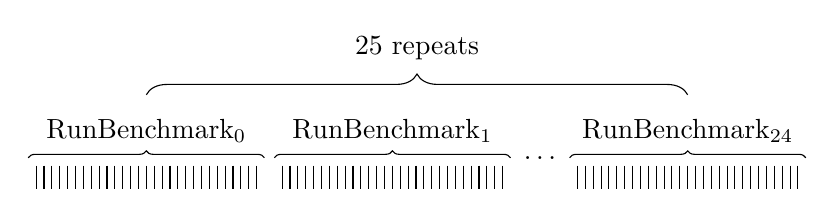
\begin{tikzpicture}[scale=1]
    \draw[decorate, decoration={brace}, align=center, shift={(0, 0)}] (0, 0) -- node[above=2] {$\textrm{\code{RunBenchmark}}_0$} +(3, 0);
    \draw[decorate, decoration={brace}, align=center, shift={(3.125, 0)}] (0, 0) -- node[above=2] {$\textrm{\code{RunBenchmark}}_1$} +(3, 0);
    \node[shift={(6.5, 0)}] {$\ldots$};
    \draw[decorate, decoration={brace}, align=center, shift={(6.875, 0)}] (0, 0) -- node[above=2] {$\textrm{\code{RunBenchmark}}_{24}$} +(3, 0);
    \draw[decorate, decoration={brace,amplitude=7.5}, align=center, shift={(1.5, .8)}] (0, 0) -- node[above=9] {25 repeats} +(6.875, 0);
    \foreach \x in { 0, 3.125, 6.875 }
    {
      \pgfmathsetmacro{\xStart}{\x + 0.1}
      \foreach \i in {0,...,28}
      {
        \draw[shift={(\xStart + \i * 0.1, -0.1)}] (0, 0) -- +(0, -0.3);
      }
    }
  \end{tikzpicture}
  \caption{Experiment execution process.}
  \label{fig:execution}
\end{figure}

One measurement is the result of executing \code{RunBenchmark} once.
In \rfig{execution}, producing one measurement corresponds to a single of the lower braces labeled ``$\textrm{\code{RunBenchmark}}_i$''.
A total of 25 measurements are produced in this way, corresponding to the upper brace in \rfig{execution}, to reduce the impact of system fluctuations in any execution.
Repetitions vary $n$ slightly because the timing iterations may produce slightly different overall times, changing the final multiplier.

Each measurement produces two values alongside the iteration count: the mean \gls{cpu} execution time and the mean of the number of cycles required by each kernel execution.
Vertical bars in plots represent the mean number of cycles and the attached error bars represent the 95\% confidence interval across the 25 repetitions.
Tables accompany each plot with mean iteration count ($n$), mean \gls{cpu} time, mean number of cycles, and their respective confidence intervals.

As an extra precaution against system fluctuations, all kernels execute in a random order, producing a single measurement before having their order reshuffled.
Specifially, the process is as follows:
\begin{enumerate*}[itemjoin={{; }}, itemjoin*={{; }}, label=(\arabic*), after={.}]
  \item shuffle all kernels
  \item execute \code{RunBenchmark} for each kernel once, producing a single measurement for each kernel
  \item repeat (1) and (2) until 25 measurements have been produced
\end{enumerate*}

\subsection{Human-Crafted Assembly Code}
The following sections compare matrix-multiplication-kernel assembly code generated by the compiler backend with human-crafted assembly code.
Moreira \etal describe both the human-crafted assembly code kernel created by a team of \gls{ibm} engineers and the methodology for producing that kernel~\autocite{moreira2021matrix}.
They present information about \gls{mma} as well as early results comparing the performance of several kernels when compiled with \gls{mma} and \gls{vsx} on \gls{power10} and \gls{power}9.
The kernels used for comparison in this thesis are updated and improved versions that were provided by the authors of that report.

\subsection{Types Missing From Analysis}
The performance analysis in this section does not include the types \code{i4} and \code{bfloat} because of limitations in the backend code generator and the microkernel code generation for \code{double} is not within the scope of this thesis.
The \code{i4} and \code{bfloat} types use the same \gls{ir} code-generation code paths and the same logic as every other type except \code{double}.
Thus, the code generated for them is  likely to be functional and as performant as the code for these other types.
However, while translating to assembly, the backend produces incorrect code for \code{i4} or an error when using \code{bfloat}.
Both issues have been acknowledged by the developer team and will be fixed in future versions of \gls{llvm}.

For \code{double}, the addition of a new operand to the instruction, as described in \rsec{doubles}, cause a significant divergence in code-generation logic that otherwise applies to all other types usable with \gls{mma}.
Within the scope of this thesis, the development efforts focus on an algorithm that worked for six of the seven types.
The method presented in \rcha{method} applies to \code{double} but its \gls{lowering} implementation will require changes in relation to the original code.

\section{Caveats}
\label{sec:caveats}
There are some unexpected performance results reported in the experiments detailed in the remaining sections of this chapter.
The unexpected performance is caused either by issues in the backend code generator or by limitations inherent to the compilation framework, both of which are outside of the scope of this thesis.

Before presenting the results, this section discusses some of the causes for the unexpected performance results.
These issues are addressable in the future and the performance study in this thesis uncovered opportunities for improving code generation for the entire \gls{power} software stack.
The presented \gls{mma} kernel is a new type of kernel never before seen by the backend and therefore the assembly code generation has not been as tuned as other kernels have been.
Only after stripping away certain bottlenecks present in the naive kernel can we learn about new issues that are still to be addressed by the backend design team.

\subsection{Spilling}
In compiler terminology, a \gls{live} value is a value that may be used by a statement in the future.
Ideally, once a value is brought from memory into a register or it is computed and placed into a register, it should remain in the register until it is \gls{dead} --- a value is dead when it is guaranteed that it will never be used again.
However, there are often not enough registers available in an architecture to keep all live values in register.
Therefore, the compiler performs analysis to decide how to judiciously select some live values to be temporarily \glslink{spill}{spilled} to memory in order to temporarily free registers for new values.
Thus, \glslink{spill}{spilling} occurs when new values must be brought from memory but all registers at that \gls{point} in the program have a \gls{live} value.
For small matrix-multiplication kernels, all values may be resident in register simultaneously or may only be used once and thus do no remain \gls{live} across future loads.
Efficient spilling requires careful scheduling but in the case of \gls{mma} the problem is made more difficult by the following issues.

\subsubsection{Framework Vector Loads}
The implementation described in \rcha{method} is integrated within a pre-existing framework that provides the default vectorisation \gls{lowering} method described in \rsec{matMulInt}.
This framework contains data structures to support operations with matrices.
These data structures transform the load of a single long vector representing a flattened matrix into several vector loads representing the matrix's column or row vectors, depending on the original access order.
For example, a floating-point column-major matrix \mat{A}{4}{2} is originally represented by \code{<8 x float>} and then transformed into two \code{<4 x float>} column-vector loads.
After the transformation, these load instructions in the \gls{ir} remain consecutive and occur before any computation.
An examination of the assembly code generated by the backend reveals that such a program is translated by the backend into assembly that brings \emph{all} of the matrix's elements to registers immediately and consecutively.
Given that
\begin{enumerate*}[itemjoin={{; }}, itemjoin*={{; or }}, label=(\arabic*), after={,}]
  \item the matrix may be larger than all available registers
  \item some registers may contain values from other matrices
\end{enumerate*}
many of the loaded values are immediately \glslink{spill}{spilled} back to memory.
These values must be reloaded later when they are needed, effectively tripling the time spent on memory accesses.
Memory operations are considerably slower than \gls{mma} operations, even though the values may be going to and from the L1 cache, and thus the runtime of the kernel becomes dominated by memory operations.

\begin{figure}[t]
  \centering
  %% Creator: Matplotlib, PGF backend
%%
%% To include the figure in your LaTeX document, write
%%   \input{<filename>.pgf}
%%
%% Make sure the required packages are loaded in your preamble
%%   \usepackage{pgf}
%%
%% Figures using additional raster images can only be included by \input if
%% they are in the same directory as the main LaTeX file. For loading figures
%% from other directories you can use the `import` package
%%   \usepackage{import}
%%
%% and then include the figures with
%%   \import{<path to file>}{<filename>.pgf}
%%
%% Matplotlib used the following preamble
%%
\begingroup%
\makeatletter%
\begin{pgfpicture}%
\pgfpathrectangle{\pgfpointorigin}{\pgfqpoint{5.501070in}{3.000000in}}%
\pgfusepath{use as bounding box, clip}%
\begin{pgfscope}%
\pgfsetbuttcap%
\pgfsetmiterjoin%
\definecolor{currentfill}{rgb}{1.000000,1.000000,1.000000}%
\pgfsetfillcolor{currentfill}%
\pgfsetlinewidth{0.000000pt}%
\definecolor{currentstroke}{rgb}{1.000000,1.000000,1.000000}%
\pgfsetstrokecolor{currentstroke}%
\pgfsetdash{}{0pt}%
\pgfpathmoveto{\pgfqpoint{0.000000in}{0.000000in}}%
\pgfpathlineto{\pgfqpoint{5.501070in}{0.000000in}}%
\pgfpathlineto{\pgfqpoint{5.501070in}{3.000000in}}%
\pgfpathlineto{\pgfqpoint{0.000000in}{3.000000in}}%
\pgfpathclose%
\pgfusepath{fill}%
\end{pgfscope}%
\begin{pgfscope}%
\pgfsetbuttcap%
\pgfsetmiterjoin%
\definecolor{currentfill}{rgb}{1.000000,1.000000,1.000000}%
\pgfsetfillcolor{currentfill}%
\pgfsetlinewidth{0.000000pt}%
\definecolor{currentstroke}{rgb}{0.000000,0.000000,0.000000}%
\pgfsetstrokecolor{currentstroke}%
\pgfsetstrokeopacity{0.000000}%
\pgfsetdash{}{0pt}%
\pgfpathmoveto{\pgfqpoint{0.794291in}{0.549691in}}%
\pgfpathlineto{\pgfqpoint{5.351070in}{0.549691in}}%
\pgfpathlineto{\pgfqpoint{5.351070in}{2.650926in}}%
\pgfpathlineto{\pgfqpoint{0.794291in}{2.650926in}}%
\pgfpathclose%
\pgfusepath{fill}%
\end{pgfscope}%
\begin{pgfscope}%
\pgfpathrectangle{\pgfqpoint{0.794291in}{0.549691in}}{\pgfqpoint{4.556779in}{2.101235in}}%
\pgfusepath{clip}%
\pgfsetbuttcap%
\pgfsetmiterjoin%
\definecolor{currentfill}{rgb}{0.121569,0.466667,0.705882}%
\pgfsetfillcolor{currentfill}%
\pgfsetlinewidth{0.000000pt}%
\definecolor{currentstroke}{rgb}{0.000000,0.000000,0.000000}%
\pgfsetstrokecolor{currentstroke}%
\pgfsetstrokeopacity{0.000000}%
\pgfsetdash{}{0pt}%
\pgfpathmoveto{\pgfqpoint{0.794291in}{0.549691in}}%
\pgfpathlineto{\pgfqpoint{1.687777in}{0.549691in}}%
\pgfpathlineto{\pgfqpoint{1.687777in}{0.822306in}}%
\pgfpathlineto{\pgfqpoint{0.794291in}{0.822306in}}%
\pgfpathclose%
\pgfusepath{fill}%
\end{pgfscope}%
\begin{pgfscope}%
\pgfpathrectangle{\pgfqpoint{0.794291in}{0.549691in}}{\pgfqpoint{4.556779in}{2.101235in}}%
\pgfusepath{clip}%
\pgfsetbuttcap%
\pgfsetmiterjoin%
\definecolor{currentfill}{rgb}{0.121569,0.466667,0.705882}%
\pgfsetfillcolor{currentfill}%
\pgfsetlinewidth{0.000000pt}%
\definecolor{currentstroke}{rgb}{0.000000,0.000000,0.000000}%
\pgfsetstrokecolor{currentstroke}%
\pgfsetstrokeopacity{0.000000}%
\pgfsetdash{}{0pt}%
\pgfpathmoveto{\pgfqpoint{3.296052in}{0.549691in}}%
\pgfpathlineto{\pgfqpoint{4.189538in}{0.549691in}}%
\pgfpathlineto{\pgfqpoint{4.189538in}{2.254402in}}%
\pgfpathlineto{\pgfqpoint{3.296052in}{2.254402in}}%
\pgfpathclose%
\pgfusepath{fill}%
\end{pgfscope}%
\begin{pgfscope}%
\pgfpathrectangle{\pgfqpoint{0.794291in}{0.549691in}}{\pgfqpoint{4.556779in}{2.101235in}}%
\pgfusepath{clip}%
\pgfsetbuttcap%
\pgfsetmiterjoin%
\definecolor{currentfill}{rgb}{1.000000,0.498039,0.054902}%
\pgfsetfillcolor{currentfill}%
\pgfsetlinewidth{0.000000pt}%
\definecolor{currentstroke}{rgb}{0.000000,0.000000,0.000000}%
\pgfsetstrokecolor{currentstroke}%
\pgfsetstrokeopacity{0.000000}%
\pgfsetdash{}{0pt}%
\pgfpathmoveto{\pgfqpoint{1.687777in}{0.549691in}}%
\pgfpathlineto{\pgfqpoint{2.581263in}{0.549691in}}%
\pgfpathlineto{\pgfqpoint{2.581263in}{0.618132in}}%
\pgfpathlineto{\pgfqpoint{1.687777in}{0.618132in}}%
\pgfpathclose%
\pgfusepath{fill}%
\end{pgfscope}%
\begin{pgfscope}%
\pgfpathrectangle{\pgfqpoint{0.794291in}{0.549691in}}{\pgfqpoint{4.556779in}{2.101235in}}%
\pgfusepath{clip}%
\pgfsetbuttcap%
\pgfsetmiterjoin%
\definecolor{currentfill}{rgb}{1.000000,0.498039,0.054902}%
\pgfsetfillcolor{currentfill}%
\pgfsetlinewidth{0.000000pt}%
\definecolor{currentstroke}{rgb}{0.000000,0.000000,0.000000}%
\pgfsetstrokecolor{currentstroke}%
\pgfsetstrokeopacity{0.000000}%
\pgfsetdash{}{0pt}%
\pgfpathmoveto{\pgfqpoint{4.189538in}{0.549691in}}%
\pgfpathlineto{\pgfqpoint{5.083024in}{0.549691in}}%
\pgfpathlineto{\pgfqpoint{5.083024in}{2.459905in}}%
\pgfpathlineto{\pgfqpoint{4.189538in}{2.459905in}}%
\pgfpathclose%
\pgfusepath{fill}%
\end{pgfscope}%
\begin{pgfscope}%
\pgfsetbuttcap%
\pgfsetroundjoin%
\definecolor{currentfill}{rgb}{0.000000,0.000000,0.000000}%
\pgfsetfillcolor{currentfill}%
\pgfsetlinewidth{0.803000pt}%
\definecolor{currentstroke}{rgb}{0.000000,0.000000,0.000000}%
\pgfsetstrokecolor{currentstroke}%
\pgfsetdash{}{0pt}%
\pgfsys@defobject{currentmarker}{\pgfqpoint{0.000000in}{-0.048611in}}{\pgfqpoint{0.000000in}{0.000000in}}{%
\pgfpathmoveto{\pgfqpoint{0.000000in}{0.000000in}}%
\pgfpathlineto{\pgfqpoint{0.000000in}{-0.048611in}}%
\pgfusepath{stroke,fill}%
}%
\begin{pgfscope}%
\pgfsys@transformshift{1.687777in}{0.549691in}%
\pgfsys@useobject{currentmarker}{}%
\end{pgfscope}%
\end{pgfscope}%
\begin{pgfscope}%
\definecolor{textcolor}{rgb}{0.000000,0.000000,0.000000}%
\pgfsetstrokecolor{textcolor}%
\pgfsetfillcolor{textcolor}%
\pgftext[x=1.687777in,y=0.452469in,,top]{\color{textcolor}\rmfamily\fontsize{10.000000}{12.000000}\selectfont 8x8x16}%
\end{pgfscope}%
\begin{pgfscope}%
\pgfsetbuttcap%
\pgfsetroundjoin%
\definecolor{currentfill}{rgb}{0.000000,0.000000,0.000000}%
\pgfsetfillcolor{currentfill}%
\pgfsetlinewidth{0.803000pt}%
\definecolor{currentstroke}{rgb}{0.000000,0.000000,0.000000}%
\pgfsetstrokecolor{currentstroke}%
\pgfsetdash{}{0pt}%
\pgfsys@defobject{currentmarker}{\pgfqpoint{0.000000in}{-0.048611in}}{\pgfqpoint{0.000000in}{0.000000in}}{%
\pgfpathmoveto{\pgfqpoint{0.000000in}{0.000000in}}%
\pgfpathlineto{\pgfqpoint{0.000000in}{-0.048611in}}%
\pgfusepath{stroke,fill}%
}%
\begin{pgfscope}%
\pgfsys@transformshift{4.189538in}{0.549691in}%
\pgfsys@useobject{currentmarker}{}%
\end{pgfscope}%
\end{pgfscope}%
\begin{pgfscope}%
\definecolor{textcolor}{rgb}{0.000000,0.000000,0.000000}%
\pgfsetstrokecolor{textcolor}%
\pgfsetfillcolor{textcolor}%
\pgftext[x=4.189538in,y=0.452469in,,top]{\color{textcolor}\rmfamily\fontsize{10.000000}{12.000000}\selectfont 32x8x32}%
\end{pgfscope}%
\begin{pgfscope}%
\definecolor{textcolor}{rgb}{0.000000,0.000000,0.000000}%
\pgfsetstrokecolor{textcolor}%
\pgfsetfillcolor{textcolor}%
\pgftext[x=3.072680in,y=0.273457in,,top]{\color{textcolor}\rmfamily\fontsize{10.000000}{12.000000}\selectfont Kernel Size}%
\end{pgfscope}%
\begin{pgfscope}%
\pgfsetbuttcap%
\pgfsetroundjoin%
\definecolor{currentfill}{rgb}{0.000000,0.000000,0.000000}%
\pgfsetfillcolor{currentfill}%
\pgfsetlinewidth{0.803000pt}%
\definecolor{currentstroke}{rgb}{0.000000,0.000000,0.000000}%
\pgfsetstrokecolor{currentstroke}%
\pgfsetdash{}{0pt}%
\pgfsys@defobject{currentmarker}{\pgfqpoint{-0.048611in}{0.000000in}}{\pgfqpoint{-0.000000in}{0.000000in}}{%
\pgfpathmoveto{\pgfqpoint{-0.000000in}{0.000000in}}%
\pgfpathlineto{\pgfqpoint{-0.048611in}{0.000000in}}%
\pgfusepath{stroke,fill}%
}%
\begin{pgfscope}%
\pgfsys@transformshift{0.794291in}{0.549691in}%
\pgfsys@useobject{currentmarker}{}%
\end{pgfscope}%
\end{pgfscope}%
\begin{pgfscope}%
\definecolor{textcolor}{rgb}{0.000000,0.000000,0.000000}%
\pgfsetstrokecolor{textcolor}%
\pgfsetfillcolor{textcolor}%
\pgftext[x=0.627624in, y=0.501466in, left, base]{\color{textcolor}\rmfamily\fontsize{10.000000}{12.000000}\selectfont \(\displaystyle {0}\)}%
\end{pgfscope}%
\begin{pgfscope}%
\pgfsetbuttcap%
\pgfsetroundjoin%
\definecolor{currentfill}{rgb}{0.000000,0.000000,0.000000}%
\pgfsetfillcolor{currentfill}%
\pgfsetlinewidth{0.803000pt}%
\definecolor{currentstroke}{rgb}{0.000000,0.000000,0.000000}%
\pgfsetstrokecolor{currentstroke}%
\pgfsetdash{}{0pt}%
\pgfsys@defobject{currentmarker}{\pgfqpoint{-0.048611in}{0.000000in}}{\pgfqpoint{-0.000000in}{0.000000in}}{%
\pgfpathmoveto{\pgfqpoint{-0.000000in}{0.000000in}}%
\pgfpathlineto{\pgfqpoint{-0.048611in}{0.000000in}}%
\pgfusepath{stroke,fill}%
}%
\begin{pgfscope}%
\pgfsys@transformshift{0.794291in}{1.077645in}%
\pgfsys@useobject{currentmarker}{}%
\end{pgfscope}%
\end{pgfscope}%
\begin{pgfscope}%
\definecolor{textcolor}{rgb}{0.000000,0.000000,0.000000}%
\pgfsetstrokecolor{textcolor}%
\pgfsetfillcolor{textcolor}%
\pgftext[x=0.488734in, y=1.029419in, left, base]{\color{textcolor}\rmfamily\fontsize{10.000000}{12.000000}\selectfont \(\displaystyle {220}\)}%
\end{pgfscope}%
\begin{pgfscope}%
\pgfsetbuttcap%
\pgfsetroundjoin%
\definecolor{currentfill}{rgb}{0.000000,0.000000,0.000000}%
\pgfsetfillcolor{currentfill}%
\pgfsetlinewidth{0.803000pt}%
\definecolor{currentstroke}{rgb}{0.000000,0.000000,0.000000}%
\pgfsetstrokecolor{currentstroke}%
\pgfsetdash{}{0pt}%
\pgfsys@defobject{currentmarker}{\pgfqpoint{-0.048611in}{0.000000in}}{\pgfqpoint{-0.000000in}{0.000000in}}{%
\pgfpathmoveto{\pgfqpoint{-0.000000in}{0.000000in}}%
\pgfpathlineto{\pgfqpoint{-0.048611in}{0.000000in}}%
\pgfusepath{stroke,fill}%
}%
\begin{pgfscope}%
\pgfsys@transformshift{0.794291in}{1.605598in}%
\pgfsys@useobject{currentmarker}{}%
\end{pgfscope}%
\end{pgfscope}%
\begin{pgfscope}%
\definecolor{textcolor}{rgb}{0.000000,0.000000,0.000000}%
\pgfsetstrokecolor{textcolor}%
\pgfsetfillcolor{textcolor}%
\pgftext[x=0.488734in, y=1.557373in, left, base]{\color{textcolor}\rmfamily\fontsize{10.000000}{12.000000}\selectfont \(\displaystyle {440}\)}%
\end{pgfscope}%
\begin{pgfscope}%
\pgfsetbuttcap%
\pgfsetroundjoin%
\definecolor{currentfill}{rgb}{0.000000,0.000000,0.000000}%
\pgfsetfillcolor{currentfill}%
\pgfsetlinewidth{0.803000pt}%
\definecolor{currentstroke}{rgb}{0.000000,0.000000,0.000000}%
\pgfsetstrokecolor{currentstroke}%
\pgfsetdash{}{0pt}%
\pgfsys@defobject{currentmarker}{\pgfqpoint{-0.048611in}{0.000000in}}{\pgfqpoint{-0.000000in}{0.000000in}}{%
\pgfpathmoveto{\pgfqpoint{-0.000000in}{0.000000in}}%
\pgfpathlineto{\pgfqpoint{-0.048611in}{0.000000in}}%
\pgfusepath{stroke,fill}%
}%
\begin{pgfscope}%
\pgfsys@transformshift{0.794291in}{2.133552in}%
\pgfsys@useobject{currentmarker}{}%
\end{pgfscope}%
\end{pgfscope}%
\begin{pgfscope}%
\definecolor{textcolor}{rgb}{0.000000,0.000000,0.000000}%
\pgfsetstrokecolor{textcolor}%
\pgfsetfillcolor{textcolor}%
\pgftext[x=0.488734in, y=2.085327in, left, base]{\color{textcolor}\rmfamily\fontsize{10.000000}{12.000000}\selectfont \(\displaystyle {660}\)}%
\end{pgfscope}%
\begin{pgfscope}%
\definecolor{textcolor}{rgb}{0.000000,0.000000,0.000000}%
\pgfsetstrokecolor{textcolor}%
\pgfsetfillcolor{textcolor}%
\pgftext[x=0.246451in, y=1.338927in, left, base,rotate=90.000000]{\color{textcolor}\rmfamily\fontsize{10.000000}{12.000000}\selectfont Runtime}%
\end{pgfscope}%
\begin{pgfscope}%
\definecolor{textcolor}{rgb}{0.000000,0.000000,0.000000}%
\pgfsetstrokecolor{textcolor}%
\pgfsetfillcolor{textcolor}%
\pgftext[x=0.398457in, y=1.480324in, left, base,rotate=90.000000]{\color{textcolor}\rmfamily\fontsize{10.000000}{12.000000}\selectfont (ns)}%
\end{pgfscope}%
\begin{pgfscope}%
\pgfpathrectangle{\pgfqpoint{0.794291in}{0.549691in}}{\pgfqpoint{4.556779in}{2.101235in}}%
\pgfusepath{clip}%
\pgfsetbuttcap%
\pgfsetroundjoin%
\pgfsetlinewidth{1.505625pt}%
\definecolor{currentstroke}{rgb}{0.000000,0.000000,0.000000}%
\pgfsetstrokecolor{currentstroke}%
\pgfsetdash{}{0pt}%
\pgfpathmoveto{\pgfqpoint{1.241034in}{0.821843in}}%
\pgfpathlineto{\pgfqpoint{1.241034in}{0.822769in}}%
\pgfusepath{stroke}%
\end{pgfscope}%
\begin{pgfscope}%
\pgfpathrectangle{\pgfqpoint{0.794291in}{0.549691in}}{\pgfqpoint{4.556779in}{2.101235in}}%
\pgfusepath{clip}%
\pgfsetbuttcap%
\pgfsetroundjoin%
\pgfsetlinewidth{1.505625pt}%
\definecolor{currentstroke}{rgb}{0.000000,0.000000,0.000000}%
\pgfsetstrokecolor{currentstroke}%
\pgfsetdash{}{0pt}%
\pgfpathmoveto{\pgfqpoint{3.742795in}{2.253898in}}%
\pgfpathlineto{\pgfqpoint{3.742795in}{2.254906in}}%
\pgfusepath{stroke}%
\end{pgfscope}%
\begin{pgfscope}%
\pgfpathrectangle{\pgfqpoint{0.794291in}{0.549691in}}{\pgfqpoint{4.556779in}{2.101235in}}%
\pgfusepath{clip}%
\pgfsetbuttcap%
\pgfsetroundjoin%
\pgfsetlinewidth{1.505625pt}%
\definecolor{currentstroke}{rgb}{0.000000,0.000000,0.000000}%
\pgfsetstrokecolor{currentstroke}%
\pgfsetdash{}{0pt}%
\pgfpathmoveto{\pgfqpoint{2.134520in}{0.617850in}}%
\pgfpathlineto{\pgfqpoint{2.134520in}{0.618414in}}%
\pgfusepath{stroke}%
\end{pgfscope}%
\begin{pgfscope}%
\pgfpathrectangle{\pgfqpoint{0.794291in}{0.549691in}}{\pgfqpoint{4.556779in}{2.101235in}}%
\pgfusepath{clip}%
\pgfsetbuttcap%
\pgfsetroundjoin%
\pgfsetlinewidth{1.505625pt}%
\definecolor{currentstroke}{rgb}{0.000000,0.000000,0.000000}%
\pgfsetstrokecolor{currentstroke}%
\pgfsetdash{}{0pt}%
\pgfpathmoveto{\pgfqpoint{4.636281in}{2.454448in}}%
\pgfpathlineto{\pgfqpoint{4.636281in}{2.465361in}}%
\pgfusepath{stroke}%
\end{pgfscope}%
\begin{pgfscope}%
\pgfpathrectangle{\pgfqpoint{0.794291in}{0.549691in}}{\pgfqpoint{4.556779in}{2.101235in}}%
\pgfusepath{clip}%
\pgfsetbuttcap%
\pgfsetroundjoin%
\definecolor{currentfill}{rgb}{0.000000,0.000000,0.000000}%
\pgfsetfillcolor{currentfill}%
\pgfsetlinewidth{1.003750pt}%
\definecolor{currentstroke}{rgb}{0.000000,0.000000,0.000000}%
\pgfsetstrokecolor{currentstroke}%
\pgfsetdash{}{0pt}%
\pgfsys@defobject{currentmarker}{\pgfqpoint{-0.010417in}{-0.000000in}}{\pgfqpoint{0.010417in}{0.000000in}}{%
\pgfpathmoveto{\pgfqpoint{0.010417in}{-0.000000in}}%
\pgfpathlineto{\pgfqpoint{-0.010417in}{0.000000in}}%
\pgfusepath{stroke,fill}%
}%
\begin{pgfscope}%
\pgfsys@transformshift{1.241034in}{0.821843in}%
\pgfsys@useobject{currentmarker}{}%
\end{pgfscope}%
\begin{pgfscope}%
\pgfsys@transformshift{3.742795in}{2.253898in}%
\pgfsys@useobject{currentmarker}{}%
\end{pgfscope}%
\end{pgfscope}%
\begin{pgfscope}%
\pgfpathrectangle{\pgfqpoint{0.794291in}{0.549691in}}{\pgfqpoint{4.556779in}{2.101235in}}%
\pgfusepath{clip}%
\pgfsetbuttcap%
\pgfsetroundjoin%
\definecolor{currentfill}{rgb}{0.000000,0.000000,0.000000}%
\pgfsetfillcolor{currentfill}%
\pgfsetlinewidth{1.003750pt}%
\definecolor{currentstroke}{rgb}{0.000000,0.000000,0.000000}%
\pgfsetstrokecolor{currentstroke}%
\pgfsetdash{}{0pt}%
\pgfsys@defobject{currentmarker}{\pgfqpoint{-0.010417in}{-0.000000in}}{\pgfqpoint{0.010417in}{0.000000in}}{%
\pgfpathmoveto{\pgfqpoint{0.010417in}{-0.000000in}}%
\pgfpathlineto{\pgfqpoint{-0.010417in}{0.000000in}}%
\pgfusepath{stroke,fill}%
}%
\begin{pgfscope}%
\pgfsys@transformshift{1.241034in}{0.822769in}%
\pgfsys@useobject{currentmarker}{}%
\end{pgfscope}%
\begin{pgfscope}%
\pgfsys@transformshift{3.742795in}{2.254906in}%
\pgfsys@useobject{currentmarker}{}%
\end{pgfscope}%
\end{pgfscope}%
\begin{pgfscope}%
\pgfpathrectangle{\pgfqpoint{0.794291in}{0.549691in}}{\pgfqpoint{4.556779in}{2.101235in}}%
\pgfusepath{clip}%
\pgfsetbuttcap%
\pgfsetroundjoin%
\definecolor{currentfill}{rgb}{0.000000,0.000000,0.000000}%
\pgfsetfillcolor{currentfill}%
\pgfsetlinewidth{1.003750pt}%
\definecolor{currentstroke}{rgb}{0.000000,0.000000,0.000000}%
\pgfsetstrokecolor{currentstroke}%
\pgfsetdash{}{0pt}%
\pgfsys@defobject{currentmarker}{\pgfqpoint{-0.010417in}{-0.000000in}}{\pgfqpoint{0.010417in}{0.000000in}}{%
\pgfpathmoveto{\pgfqpoint{0.010417in}{-0.000000in}}%
\pgfpathlineto{\pgfqpoint{-0.010417in}{0.000000in}}%
\pgfusepath{stroke,fill}%
}%
\begin{pgfscope}%
\pgfsys@transformshift{2.134520in}{0.617850in}%
\pgfsys@useobject{currentmarker}{}%
\end{pgfscope}%
\begin{pgfscope}%
\pgfsys@transformshift{4.636281in}{2.454448in}%
\pgfsys@useobject{currentmarker}{}%
\end{pgfscope}%
\end{pgfscope}%
\begin{pgfscope}%
\pgfpathrectangle{\pgfqpoint{0.794291in}{0.549691in}}{\pgfqpoint{4.556779in}{2.101235in}}%
\pgfusepath{clip}%
\pgfsetbuttcap%
\pgfsetroundjoin%
\definecolor{currentfill}{rgb}{0.000000,0.000000,0.000000}%
\pgfsetfillcolor{currentfill}%
\pgfsetlinewidth{1.003750pt}%
\definecolor{currentstroke}{rgb}{0.000000,0.000000,0.000000}%
\pgfsetstrokecolor{currentstroke}%
\pgfsetdash{}{0pt}%
\pgfsys@defobject{currentmarker}{\pgfqpoint{-0.010417in}{-0.000000in}}{\pgfqpoint{0.010417in}{0.000000in}}{%
\pgfpathmoveto{\pgfqpoint{0.010417in}{-0.000000in}}%
\pgfpathlineto{\pgfqpoint{-0.010417in}{0.000000in}}%
\pgfusepath{stroke,fill}%
}%
\begin{pgfscope}%
\pgfsys@transformshift{2.134520in}{0.618414in}%
\pgfsys@useobject{currentmarker}{}%
\end{pgfscope}%
\begin{pgfscope}%
\pgfsys@transformshift{4.636281in}{2.465361in}%
\pgfsys@useobject{currentmarker}{}%
\end{pgfscope}%
\end{pgfscope}%
\begin{pgfscope}%
\pgfsetrectcap%
\pgfsetmiterjoin%
\pgfsetlinewidth{0.803000pt}%
\definecolor{currentstroke}{rgb}{0.000000,0.000000,0.000000}%
\pgfsetstrokecolor{currentstroke}%
\pgfsetdash{}{0pt}%
\pgfpathmoveto{\pgfqpoint{0.794291in}{0.549691in}}%
\pgfpathlineto{\pgfqpoint{0.794291in}{2.650926in}}%
\pgfusepath{stroke}%
\end{pgfscope}%
\begin{pgfscope}%
\pgfsetrectcap%
\pgfsetmiterjoin%
\pgfsetlinewidth{0.803000pt}%
\definecolor{currentstroke}{rgb}{0.000000,0.000000,0.000000}%
\pgfsetstrokecolor{currentstroke}%
\pgfsetdash{}{0pt}%
\pgfpathmoveto{\pgfqpoint{5.351070in}{0.549691in}}%
\pgfpathlineto{\pgfqpoint{5.351070in}{2.650926in}}%
\pgfusepath{stroke}%
\end{pgfscope}%
\begin{pgfscope}%
\pgfsetrectcap%
\pgfsetmiterjoin%
\pgfsetlinewidth{0.803000pt}%
\definecolor{currentstroke}{rgb}{0.000000,0.000000,0.000000}%
\pgfsetstrokecolor{currentstroke}%
\pgfsetdash{}{0pt}%
\pgfpathmoveto{\pgfqpoint{0.794291in}{0.549691in}}%
\pgfpathlineto{\pgfqpoint{5.351070in}{0.549691in}}%
\pgfusepath{stroke}%
\end{pgfscope}%
\begin{pgfscope}%
\pgfsetrectcap%
\pgfsetmiterjoin%
\pgfsetlinewidth{0.803000pt}%
\definecolor{currentstroke}{rgb}{0.000000,0.000000,0.000000}%
\pgfsetstrokecolor{currentstroke}%
\pgfsetdash{}{0pt}%
\pgfpathmoveto{\pgfqpoint{0.794291in}{2.650926in}}%
\pgfpathlineto{\pgfqpoint{5.351070in}{2.650926in}}%
\pgfusepath{stroke}%
\end{pgfscope}%
\begin{pgfscope}%
\definecolor{textcolor}{rgb}{0.000000,0.000000,0.000000}%
\pgfsetstrokecolor{textcolor}%
\pgfsetfillcolor{textcolor}%
\pgftext[x=3.072680in,y=2.734260in,,base]{\color{textcolor}\rmfamily\fontsize{12.000000}{14.400000}\selectfont Effect of Load Sinking on Float Matrices}%
\end{pgfscope}%
\begin{pgfscope}%
\pgfsetbuttcap%
\pgfsetmiterjoin%
\definecolor{currentfill}{rgb}{1.000000,1.000000,1.000000}%
\pgfsetfillcolor{currentfill}%
\pgfsetfillopacity{0.800000}%
\pgfsetlinewidth{1.003750pt}%
\definecolor{currentstroke}{rgb}{0.800000,0.800000,0.800000}%
\pgfsetstrokecolor{currentstroke}%
\pgfsetstrokeopacity{0.800000}%
\pgfsetdash{}{0pt}%
\pgfpathmoveto{\pgfqpoint{0.891513in}{2.152470in}}%
\pgfpathlineto{\pgfqpoint{1.795063in}{2.152470in}}%
\pgfpathquadraticcurveto{\pgfqpoint{1.822841in}{2.152470in}}{\pgfqpoint{1.822841in}{2.180247in}}%
\pgfpathlineto{\pgfqpoint{1.822841in}{2.553704in}}%
\pgfpathquadraticcurveto{\pgfqpoint{1.822841in}{2.581482in}}{\pgfqpoint{1.795063in}{2.581482in}}%
\pgfpathlineto{\pgfqpoint{0.891513in}{2.581482in}}%
\pgfpathquadraticcurveto{\pgfqpoint{0.863735in}{2.581482in}}{\pgfqpoint{0.863735in}{2.553704in}}%
\pgfpathlineto{\pgfqpoint{0.863735in}{2.180247in}}%
\pgfpathquadraticcurveto{\pgfqpoint{0.863735in}{2.152470in}}{\pgfqpoint{0.891513in}{2.152470in}}%
\pgfpathclose%
\pgfusepath{stroke,fill}%
\end{pgfscope}%
\begin{pgfscope}%
\pgfsetbuttcap%
\pgfsetmiterjoin%
\definecolor{currentfill}{rgb}{0.121569,0.466667,0.705882}%
\pgfsetfillcolor{currentfill}%
\pgfsetlinewidth{0.000000pt}%
\definecolor{currentstroke}{rgb}{0.000000,0.000000,0.000000}%
\pgfsetstrokecolor{currentstroke}%
\pgfsetstrokeopacity{0.000000}%
\pgfsetdash{}{0pt}%
\pgfpathmoveto{\pgfqpoint{0.919291in}{2.428704in}}%
\pgfpathlineto{\pgfqpoint{1.197068in}{2.428704in}}%
\pgfpathlineto{\pgfqpoint{1.197068in}{2.525926in}}%
\pgfpathlineto{\pgfqpoint{0.919291in}{2.525926in}}%
\pgfpathclose%
\pgfusepath{fill}%
\end{pgfscope}%
\begin{pgfscope}%
\definecolor{textcolor}{rgb}{0.000000,0.000000,0.000000}%
\pgfsetstrokecolor{textcolor}%
\pgfsetfillcolor{textcolor}%
\pgftext[x=1.308180in,y=2.428704in,left,base]{\color{textcolor}\rmfamily\fontsize{10.000000}{12.000000}\selectfont No Opt}%
\end{pgfscope}%
\begin{pgfscope}%
\pgfsetbuttcap%
\pgfsetmiterjoin%
\definecolor{currentfill}{rgb}{1.000000,0.498039,0.054902}%
\pgfsetfillcolor{currentfill}%
\pgfsetlinewidth{0.000000pt}%
\definecolor{currentstroke}{rgb}{0.000000,0.000000,0.000000}%
\pgfsetstrokecolor{currentstroke}%
\pgfsetstrokeopacity{0.000000}%
\pgfsetdash{}{0pt}%
\pgfpathmoveto{\pgfqpoint{0.919291in}{2.235031in}}%
\pgfpathlineto{\pgfqpoint{1.197068in}{2.235031in}}%
\pgfpathlineto{\pgfqpoint{1.197068in}{2.332253in}}%
\pgfpathlineto{\pgfqpoint{0.919291in}{2.332253in}}%
\pgfpathclose%
\pgfusepath{fill}%
\end{pgfscope}%
\begin{pgfscope}%
\definecolor{textcolor}{rgb}{0.000000,0.000000,0.000000}%
\pgfsetstrokecolor{textcolor}%
\pgfsetfillcolor{textcolor}%
\pgftext[x=1.308180in,y=2.235031in,left,base]{\color{textcolor}\rmfamily\fontsize{10.000000}{12.000000}\selectfont Sink}%
\end{pgfscope}%
\end{pgfpicture}%
\makeatother%
\endgroup%

  \caption{The effect of load sinking on \code{float} and \code{i16} matrix multiplications.}
  \label{fig:floatSink}
\end{figure}
\begin{table}[t]
  \centering
  \begin{tabular}{| c | c | c | c | c | c |}
    \hline
    Type & Size & \parbox[t][26pt][t]{40pt}{\centering Load\\Sinking} & \parbox[t][26pt][t]{50pt}{\centering$n$\\(millions)} & \parbox[t][28pt][t]{60pt}{\centering CPU Time\\(\SI{}{\textit{\nano\second}})} & Cycles\\\hline
    \code{float} & small & no & $25.6 \pm 0.62$ & $54.84 \pm 1.39$ & $219.11 \pm 5.57$ \\
    \code{float} & small & yes & $97.3 \pm 0.14$ & $14.44 \pm 0.05$ & $57.67 \pm 0.19$ \\
    \code{float} & large & no & $2.1 \pm 0.05$ & $654.30 \pm 14.86$ & $2614.07 \pm 59.39$ \\
    \code{float} & large & yes & $2.4 \pm 0.05$ & $596.81 \pm 13.12$ & $2384.39 \pm 52.42$ \\
    \code{i16} & small & no & $91.4 \pm 0.04$ & $15.31 \pm 0.00$ & $61.18 \pm 0.02$ \\
    \code{i16} & small & yes & $80.4 \pm 0.15$ & $17.42 \pm 0.01$ & $69.61 \pm 0.03$ \\
    \code{i16} & large & no & $3.4 \pm 0.02$ & $415.63 \pm 2.21$ & $1660.53 \pm 8.85$ \\
    \code{i16} & large & yes & $2.2 \pm 0.00$ & $627.73 \pm 2.19$ & $2507.92 \pm 8.75$ \\\hline
  \end{tabular}
  \caption{
    The effect of load sinking on \code{float} and \code{i16} matrix multiplications.
    See \rfig{floatSink} for graphical presentation.
  }
  \label{tab:floatSink}
\end{table}

This spilling issue must be resolved by the backend scheduler: the scheduler needs to move loads closer to the \gls{point} in the program that contains the first use of the loaded value to reduce register pressure by using a technique called ``load sinking.''\footnotemark
\footnotetext{The backend design team is currently investigating how to implement this change to the scheduler.}
Load sinking may not reduce register pressure in many other programs, but in the case of this matrix-multiplication kernel it certainly does.
A workaround for the spilling that results from unsunk loads, which can be used until the backend scheduler improves, consists of modifying the \gls{ir} by further breaking up the vector loads into smaller vector loads and sinking these smaller loads closer to the first use of the loaded values.

In preparation for the performance evaluation in this thesis, a short targeted \gls{ir} transformation was implemented using this tactic.
Its goal was to produce results that are more representative of the code that will be generated by a final production-ready backend.
Consider the pair of bars labeled ``$8 \times 8 \times 16$'' (\matmul{8}{8}{16}) for \code{float} (left) in \rfig{floatSink}.
This matrix size represents the best-case scenario for such an optimisation:
\begin{enumerate*}[itemjoin={{; }}, itemjoin*={{; and }}, label={\protect\circled{\arabic*}}, after={.}]
  \item $A$'s eight-element column-vector load can be broken up into two four-element vector loads, each of which fills an entire \gls{vsr} (similar logic applies to $B$'s rows)
  \item only a single load is necessary to create an outer-product operand (rank-one update)
  \item each operand is used only once during the accumulation step ($2+4=6$ registers \gls{live} at once)
\end{enumerate*}
Given such a perfect case, the runtime of the original version (labeled ``No Load Sinking'' in \rfig{floatSink}, first row in \rtab{floatSink}) is roughly quartered in the optimised version (``Load Sinking'', second row).
If the operation were to have more accumulations, then this gap should continue to grow as more and more spills would be required in the unoptimised version.

However, by examining the bars labeled ``$8 \times 8 \times 16$'' for \code{i16} (right) in \rfig{floatSink} we can see that for smaller types load sinking actually causes a slight slow down (\rtab{floatSink}, rows 5 and 6).
This slowdown can be attributed to the invalidation of properties \circled{1} and \circled{2}: loading an \code{i16} operand no longer fills an entire register and two loads are necessary to create an operand for \code{i16} (rank-two update).
In fact, the assembly produced without load sinking is much closer to the handwritten version because it loads multiple vectors into a single register and uses this register as a source for multiple shuffle instructions.
Loading multiple vectors into a single register is possible because the \gls{ir} of the version without load sinking has all of vectors being loaded simulataneously.
When lowered by the backend, this single contiguous load is automatically broken into register-sized pieces that are then, importantly, also spilled in the same format.
Thus when the \glspl{vsr} are reloaded, they contain two \code{i16} vectors.
The load-sinking version avoids spills by breaking the single contiguous load into individual vector loads, removing the \gls{ir} opportunity to have the loads merged.
It is possible for the backend to recombine the loads but this has yet to be observed in any kernel compilation.
These individual vector loads increase register pressure and each loaded \gls{vsr} is used in a single shuffle instruction.
The performance degradation because of load-sinking in this case is small only because the overall register pressure has been decreased by halving the element width.

\subsubsection{Operand Spilling and Rematerialisation}
After addressing the load-sinking issue in this way, another, separate but related, issue appears.
As can be seen from the pair of bars labeled ``$32 \times 8 \times 32$'' for \code{float} in \rfig{floatSink}, the same fix that produced significant speedup for a smaller kernel has significantly reduced in effectiveness for a larger kernel.
An examination of the assembly reveals that the large number of loads that led to spills at the beginning of the kernel prior to sinking the loads are indeed no longer there.
However, while there are no spills throughout the body of the smaller kernel, the larger kernel has multiple spills or reloads per set of outer products.
The issue here is that, for the larger kernel, property \circled{3} no longer holds true.

Consider the example in \rfig{opReuse}.
The figure shows an example large kernel ($16 \times 32$) in the style of \rfig{intrinsic}; to illustrate how spills occur, the figure does not divide individual elements nor does it show $B$.
On the right, darker lines divide the output into blocks of accumulators while the lighter lines divide blocks into the eight accumulators as in \rfig{intrinsic}.
Each of the smaller boxes on the left represents an operand composed of four \code{float} elements used in an outer-product computation.

An example operand from $A$, highlighted by parallel diagonal lines, must be used in the accumulation of the first set of accumulators, highlighted by a crosshatch pattern.
In the computation of the smaller kernel in \rfig{floatSink}, this value is now \gls{dead}.
The larger kernel, however, must use the value again in computing the second set of accumulators, highlighted by a dotted pattern.

\begin{figure}[t]
  \centering
  \begin{tikzpicture}[scale=1/2]
    \draw[xstep=1, ystep=2, shift={(0, 0)}] (0, 0) grid +(2, 8);
    \draw[pattern=north west lines, shift={(0, 6)}] (0, 0) rectangle +(1, 2);
    \draw[pattern=crosshatch, shift={(3, 6)}] (0, 0) rectangle +(8, 2);
 %   \draw[pattern={Hatch[angle=45,distance={8pt},xshift=.2pt, line width=1.25]}, shift={(3, 6)}] (0, 0) rectangle +(8, 2);
    \draw[pattern=dots, shift={(11, 6)}] (0, 0) rectangle +(8, 2);
 %   \draw[pattern={Dots[angle=45,distance={7pt},xshift=.1pt, radius=1.25]}, shift={(11, 6)}] (0, 0) rectangle +(8, 2);
    \draw[xstep=2, ystep=2, shift={(3, 0)}, color={black!20!white}] (0, 0) grid +(16, 8);
    \draw[xstep=8, ystep=4, shift={(3, 0)}] (0, 0) grid +(16, 8);
    \draw[decorate, decoration={brace, mirror}] (0, -0.3) -- node[below=2] {$K$} +(2, 0);
  \end{tikzpicture}
  \caption{Demonstration of operand reuse.}
  \label{fig:opReuse}
\end{figure}

According to constraint \fbox{5} in \rsec{baseCase}, spilling an accumulator is expensive, and therefore an efficient solution must finish computing a block of accumulators before moving on to a different area of the matrix.
Doing so requires that every operand along the dimension $K$ be brought to a register before any operand can be reused with a new block of accumulators.
For instance, an accumulator layout like that in \rfig{opReuse} requires six operand registers for each accumulation to be performed.
Using only the 32 registers available while the accumulators are assembled, if $K \geq \left\lceil \frac{32}{6} \right\rceil = 6$, then there is not enough space for all values to remain in registers.
And thus the cause for the multiple spills and reloads throughout the computation becomes apparent: operands from $A$ that are still \gls{live} are being forced out of registers and the compiler is choosing to spill them.\footnotemark
\footnotetext{The issue is identical for operands of $B$, though the reuse distance is greater.}

This code generation evokes the well-studied compiler technique ``\gls{rematerialisation}''.
Essentially, the compiler analysis must answer the question ``is it more efficient to store a value to memory and retrieve it later (\gls{spill}) or to recompute it later using the same process?''

In the case of floats, producing the operand is a simple load and therefore, if an operand \emph{must} be evicted from its register, \glslink{rematerialisation}{rematerialising} the value is a simple load.
Thus, the compiler's choice to spill the operand is incorrect and, because spills are saved on the stack, not only is it wasting memory by duplicating the value, it is also potentially evicting values from the cache.
Regardless, the larger kernel's execution, optimised or not, is significantly influenced by memory operations, though the gains from reducing the initial spills still have significant impact.

For smaller datatypes, however, spilling is the correct choice.
Materialising an \code{i16} involves two loads and at least one instruction to shuffle the loaded data together.
Rematerialising the value in the future becomes a simple load, significantly reducing register pressure and required memory bandwidth.
Both the original version and the load-sinking version correctly choose to spill their values instead of \glslink{rematerialisation}{rematerialising} them.
As with \code{float}, the increased number of memory operations explains the significant increase in execution time for the larger \code{i16} kernel in \rfig{floatSink}, but it does not, however, explain the large difference between the two version.
The next section investigates this discrepancy.

\subsubsection{Smaller Types}
While the issues affecting \code{float} matrices presented above remain roughly identical for \code{double}-typed operations, small datatypes have a separate source of slow down.
The difference in performance is actually an exacerbation of an already-discussed issue, namely the invalidation of properties \circled{1} and \circled{2}.
For \code{i16}, in the load-sinking version, a single 64-bit double-word load instruction loads four \code{i16} elements at the same time, filling only half of a vector register.
The original version loads 16 elements at a time using 256-bit vector-pair loads, meaning that the load-sinking version quadruples the number of loads required to load the values needed for the computation (excluding loads from the original spilling issue).
Changing the scheduling to remove the unnecessary loads and stores resulting from spilling would likely lead to a much more significant performance gap between the two versions.

This issue extends to the other data types, which perform rank-two, -four, or -eight updates.
The issue is aggravated when the number of memory requests increases because of the shrinking data width that requires more vectors for shuffling.
For example, where, for \code{i16}, the load-sinking version takes roughly 114\% of the execution time of the original version, the same comparison for \code{i8} shows that the load-sinking version takes 292\% of the execution time of the original version.

A more complicated load breaking and sinking strategy may counteract this slowdown, but only to a certain degree.
Combining certain loads -- for example two four-element \code{i16} column loads, making a full \gls{vsr} -- would decrease register pressure because the upper and lower halves of the register can be used in separate shuffles.
However, this still does not quite match the 256-bit paired-vector load in terms of memory-request efficiency.
It is impossible for smaller types to use this 256-bit load because the columns of $A$ are consecutive: the paired-vector load would load values that are not used until the second row of accumulator blocks, inevitably introducing new spills.

The issue worsens for \code{i8} and \code{i4} where the eight consecutive vertical elements fill less and less of a \gls{vsr}.
For larger kernels, the smaller data types thus imply a increasing number of loads, further diluting the speedup gained from \gls{mma}.

\subsection{Shuffling}
For datatypes smaller than 32 bits, producing the appropriate operand for a rank-$r$ update requires several vectors be merged via shuffling.
The \gls{power} \gls{isa} offers several methods to move vector elements, ranging from register shifting and rotating combined with masking to efficient vector upper and lower half merges based on datatype size.
Transforming \gls{ir} statements in an efficient code for shuffling is an involved design process.

There are a multitude ways to express the same shuffling operation in \gls{ir}, each depending on multiple implementation choices made throughout the process.
Certain variants are interpreted by the backend and translated to efficient code while others are interpreted very conservatively.
This discrepancy in translation can be the difference between an idiomatic assembly of several instructions, often close to Moreira \etal's handwritten version, and the same process being expressed in hundreds or thousands of instructions, often with \glspl{spill} throughout.
Several factors that lead shuffling to cause performance degradation are discussed below.

\subsubsection{Datatype: \texorpdfstring{\code{half}}{half}}
\label{sec:halfShuffle}
The \code{i16} and \code{half} types have identical widths: a halfword.
Because \glspl{cpu} and their accompanying \glspl{isa} are type-agnostic and sensitive only to the width of a data element when implementing vector shuffles, shuffle code in the \gls{ir} that differs only in choice of 16-bit type should produce identical assembly.
However, the assembly code currently generated by the compiler backend for \code{i16} executes roughly six vector loads and six vector permute instructions to produce all operands for a single accumulation in a full $2 \times 4$ accumulator layout.
For \code{half}, the generated assembly code has gone from six instructions to almost 150 instructions because the computation is partially scalarised by moving elements from vector registers to general-purpose registers and back again.

This explosion in code size is most apparent in the calculation epilogue where, in the \gls{ir}, the accumulators are disassembled and stored to memory.
First, the resulting accumulator vectors are truncated to the output data type.
They are then concatenated together into an output flattened matrix and stored to memory.
Concatenation is also achieved through shuffling and therefore experiences the same conservative code generation as before.
The added truncation operation worsens the effect.
All told, in the assembly code currently generated for \code{half}, the epilogue is roughly ten times the length of the same operation for \code{i16}.

\subsubsection{Datatype: \texorpdfstring{\code{i4}}{i4}}
For \code{i8}, degradations arise from \glspl{spill} due to extra register pressure but also from needing to merge four separate vectors (rank-four update).
Despite these degradations, the generated code is fairly close to the ideal, handwritten assembly.
The \gls{power10} \gls{isa} has instructions that merge vectors at a per-byte granularity, but not at a sub-byte granularity as is required for \code{i4} code generation.
Therefore, to shuffle a vector of \code{i4} elements using the same \gls{ir} code generation, the backend generates significantly less performant code that includes vector rotations and scalarisation, with single bytes being moved individually to and from general purpose registers.
The consequent slow down negates much of the speed up that could be achieved via the \gls{mma} rank-eight update.

\subsection{Solutions}
This section presents potential solutions to the performance degradations uncovered by the experimental evaluation.
The successful integration of these and other ideas in the compiler requires further investigation and cooperation with backend developers.

\subsubsection{Spilling}
\label{sec:spillSolution}
The simplest solution to the \glslink{spill}{spilling} issues is for developers to focus on using only small kernels and, indeed, this is not so unreasonable a proposal as one might perceive it at first.
\gls{llvm} requires that valid \gls{ir} code is always able to be lowered to assembly.
However, it does not require that the generated code be as performant as possible, as is demonstrated by the above issues with shuffling \code{i4} vectors.
Choosing to avoid larger kernels may seem like a defeatist notion but is actually a tried-and-true approach to performance in compilers: make the common case fast.

The average user interacts with a compiler through a high-level language, not its \gls{ir}.
Thus, the frontend will choose the fastest solution to implement a user's code; if the fastest implementation is a small kernel encapsulated by an outer kernel then that is what will be chosen.
With this notion, optimisation can be focused on this most common case for which a solution is known.
A larger inner-kernel will always remain usable but it will be less performant.

Furthermore, the most performant library implementations focus on using small unrolled assembly kernels, often computing kernels with dimensions of four to eight elements.
These small kernels are then surrounded by memory-managing outer kernels as described in \rsec{outerKernel}.
This strategy is used by Kuzma \etal~\autocite{kuzma2021fast} while using the inner kernel presented in this thesis with results comparable to libraries that feature kernels written in assembly.
Thus, using only smaller kernels can be seen as a well-worn path to performance.

If a larger kernel \emph{must} be used, significant investigation must be done to test load scheduling, value \gls{rematerialisation}, load breaking, and, if necessary, load recombination.
It is unlikely that such a solution will be found within the \gls{ir} because .
\begin{enumerate*}[itemjoin={{; }}, itemjoin*={{; and }}, label=(\arabic*), after={.}]
  \item it is in \gls{ssa} form which often folds identical values together without consideration for the times when a value is \gls{live}
  \item for better or worse, the backend does not have to respect \gls{ir} operation order
\end{enumerate*}
Such a solution will have to be found in the backend.

\subsubsection{Shuffling}
Unlike issues with spilling, it is likely that performance degradations caused by misbehaving shuffles can be solved by creating type-specific shuffling code.
While injecting the proposed solution code into the original vectorisation framework is possible, it would be much more effective to first refactor the framework so that such a modification is easier.

For \code{half} vectors, it may be possible for the compiler to generate code in a similar fashion as is done for \code{i16} simply by reinterpreting data as \code{i16} via casts and manipulating the data in this state.
The cast is not a conversion, simply a reinterpretation of the bits in a register and it is meaningful only within the \gls{llvm} framework.
Such casting produces no new instructions.
The data can be casted back to \code{half} at no cost when it needs to be used in a computation.
In theory, this produces much better assembly but may also trigger a very conservative response in the back-end of the compiler, worsening the code significantly with scalar element movement derived from a perceived conversion hazard.

The sub-byte granularity of \code{i4} vectors poses a different problem.
Performant shuffling code for \code{i4} in the same style as the larger types is an impossibility.
Instead, clever use of bitwise operations must explicitly be used to implement efficient element extraction and movement.
Bitwise operations can be applied across an entire vector register, removing the need for scalarisation and improving register usage by reducing the number of required intermediate registers.

\subsubsection{Evaluation Disclaimer}
The load-sinking and shuffling code transformations are not applied to any of the experimental evaluations presented in the remaining sections of this chapter because no tested transformation positively affected all cases.
Advantaging one type or one size of kernel would give a distorted view of the performance that can be achieved in the machine.
Thus, all test cases use identical \gls{ir} generation logic and are equally advantaged and disadvantaged in code generation.

\section{Data Access Orders}
\label{sec:variedOrders}
As discussed in \rsec{outerKernel}, packing is very important for matrix-multiplication performance.
An important part of packing, beyond choosing dimensions, is the choice of data access order.
\rsec{registerArguments} shows that \gls{mma} is sensitive to the access order of elements in \glspl{vsr} and, therefore, also sensitive to the access order of the matrices in memory from which values are loaded into registers.

\subsection{Setup}
When using an unmodified version of \gls{llvm}, the access orders of $A$, $B$, and $C$ are tied together and must be equal.
Thus two test cases, one all-column-major ($\textrm{C} = \textrm{C} \times \textrm{C}$) and another all-row-major ($\textrm{R} = \textrm{R} \times \textrm{R}$), constitute the baseline for the experiment.
In order to test the performance of the hypothesised best mix of orientations, further modifications to the \gls{lowering} framework were performed to enable the mixing of orientations.
With this possibility enabled, two cases are added to the comparison: both use the proposed optimal layout for $A$ and $B$ but vary the layout of $C$ ($\textrm{C} = \textrm{C} \times \textrm{R}$ and $\textrm{R} = \textrm{C} \times \textrm{R}$)

Each kernel uses a $2 \times 4$ accumulator setup and, therefore, in keeping with the suggestion in \rsec{spillSolution}, uses a small $8 \times 16$ output.
The inner most dimension of the kernel is 32, making the overall computation \matmul{8}{32}{16}.
An inner dimension of 32 requires 32 accumulations but smaller datatypes perform rank-$r$ updates, effectively reducing the number of operations required to compute the kernel.
It may seem that 32 accumulations is relatively large, but~\autocite{kuzma2021fast} determines that, even given the poor load scheduling, up to 128 accumulations per kernel gives good speed up, with performance plateauing with any more accumulations.
Given the discussion in \rsec{orderExpectation}, more accumulations implies more opportunities for a ``good'' orientation to outperform a bad orientation, effectively highlighting differences in performance.

\subsection{Expectation}
\label{sec:orderExpectation}
A column-major orientation data layout for $A$ should be optimal.
For \code{float}, a \gls{vsr}, which is a row-major $4 \times 1$ matrix according to the \gls{isa}, is indistinguishable from a single column of four elements when loaded from memory.
Thus, if $A$ is laid out in column-major order, an operand can be created with a single load and no waste.
However, if $A$ is laid out in row-major order, it is likely that $K \ne 1$ and thus the elements in the first column of $A$ are not consecutive in memory.
Therefore, to create an operand, four loads must be issued, one for each element of the operand.
Further overhead is incurred to move elements into the vector register either from scalar registers if the four scalar loads were issued or to shuffle elements from four vectors that were loaded.
Thus, a column-major order layout is highly preferred.
The same logic can be applied to $B$, except that a row-major orientation is preferred.

For smaller types, the logic is more complicated because the byte length of the overall loaded data also shrinks.
In the interest of not repeating much of the discussion in \rsec{caveats}, the same logic as above can be applied while acknowledging that as register usage efficiency decreases speedups also decrease.

An interesting point of discussion exists for types \code{i8} and \code{i4} whose in-register dimensions are $4 \times 4$ and $4 \times 8$ respectively.
With two \code{i4} elements packed into a byte, an eight-element vector only occupies four bytes and, therefore, \code{i8} and \code{i4} require loading four four-byte vectors to provide the elements to fill a \gls{vsr}.
Thus, four loads must be issued when extracting operands from either a row-major or a column-major order matrix.
In this case, either orientation is acceptable when operands are being built in isolation.
However, if several operands are being built simultaneously, loads can be combined to increase efficiency.
The need for shuffle instructions does not decrease, only the indices from which shuffles extract elements in a vector change.
This change can have a small, but noticeable, impact on the results.

The initial expectation is that $C$ should be stored in row-major orientation.
This is simply because the simplest method of using \gls{mma} places the operand from $A$ as the first argument and the operand from $B$ as the second argument in the outer product instruction.
When used in this way, the elements in the accumulator are oriented in a row-major fashion and, after disassembling, there is no extra work required before storing the underlying vectors to memory.
Transposing the values so that they can be stored into a column-major output-matrix requires extra shuffles.
However, the theorem discussed in \rsec{arbitraryOrder} states that reversing the order of the arguments causes the result in the accumulator to be equivalent but in a column-major order.
Thus, either access order can be used for $C$ without loss of performance.

\subsection{Analysis}
\begin{figure}[t]
  \centering
  %% Creator: Matplotlib, PGF backend
%%
%% To include the figure in your LaTeX document, write
%%   \input{<filename>.pgf}
%%
%% Make sure the required packages are loaded in your preamble
%%   \usepackage{pgf}
%%
%% Figures using additional raster images can only be included by \input if
%% they are in the same directory as the main LaTeX file. For loading figures
%% from other directories you can use the `import` package
%%   \usepackage{import}
%%
%% and then include the figures with
%%   \import{<path to file>}{<filename>.pgf}
%%
%% Matplotlib used the following preamble
%%
\begingroup%
\makeatletter%
\begin{pgfpicture}%
\pgfpathrectangle{\pgfpointorigin}{\pgfqpoint{5.501070in}{5.500000in}}%
\pgfusepath{use as bounding box, clip}%
\begin{pgfscope}%
\pgfsetbuttcap%
\pgfsetmiterjoin%
\definecolor{currentfill}{rgb}{1.000000,1.000000,1.000000}%
\pgfsetfillcolor{currentfill}%
\pgfsetlinewidth{0.000000pt}%
\definecolor{currentstroke}{rgb}{1.000000,1.000000,1.000000}%
\pgfsetstrokecolor{currentstroke}%
\pgfsetdash{}{0pt}%
\pgfpathmoveto{\pgfqpoint{0.000000in}{0.000000in}}%
\pgfpathlineto{\pgfqpoint{5.501070in}{0.000000in}}%
\pgfpathlineto{\pgfqpoint{5.501070in}{5.500000in}}%
\pgfpathlineto{\pgfqpoint{0.000000in}{5.500000in}}%
\pgfpathclose%
\pgfusepath{fill}%
\end{pgfscope}%
\begin{pgfscope}%
\pgfsetbuttcap%
\pgfsetmiterjoin%
\definecolor{currentfill}{rgb}{1.000000,1.000000,1.000000}%
\pgfsetfillcolor{currentfill}%
\pgfsetlinewidth{0.000000pt}%
\definecolor{currentstroke}{rgb}{0.000000,0.000000,0.000000}%
\pgfsetstrokecolor{currentstroke}%
\pgfsetstrokeopacity{0.000000}%
\pgfsetdash{}{0pt}%
\pgfpathmoveto{\pgfqpoint{0.704013in}{3.242658in}}%
\pgfpathlineto{\pgfqpoint{2.710257in}{3.242658in}}%
\pgfpathlineto{\pgfqpoint{2.710257in}{4.852779in}}%
\pgfpathlineto{\pgfqpoint{0.704013in}{4.852779in}}%
\pgfpathclose%
\pgfusepath{fill}%
\end{pgfscope}%
\begin{pgfscope}%
\pgfpathrectangle{\pgfqpoint{0.704013in}{3.242658in}}{\pgfqpoint{2.006244in}{1.610121in}}%
\pgfusepath{clip}%
\pgfsetbuttcap%
\pgfsetmiterjoin%
\definecolor{currentfill}{rgb}{0.121569,0.466667,0.705882}%
\pgfsetfillcolor{currentfill}%
\pgfsetlinewidth{0.000000pt}%
\definecolor{currentstroke}{rgb}{0.000000,0.000000,0.000000}%
\pgfsetstrokecolor{currentstroke}%
\pgfsetstrokeopacity{0.000000}%
\pgfsetdash{}{0pt}%
\pgfpathmoveto{\pgfqpoint{0.704013in}{3.242658in}}%
\pgfpathlineto{\pgfqpoint{1.097394in}{3.242658in}}%
\pgfpathlineto{\pgfqpoint{1.097394in}{4.706404in}}%
\pgfpathlineto{\pgfqpoint{0.704013in}{4.706404in}}%
\pgfpathclose%
\pgfusepath{fill}%
\end{pgfscope}%
\begin{pgfscope}%
\pgfpathrectangle{\pgfqpoint{0.704013in}{3.242658in}}{\pgfqpoint{2.006244in}{1.610121in}}%
\pgfusepath{clip}%
\pgfsetbuttcap%
\pgfsetmiterjoin%
\definecolor{currentfill}{rgb}{0.121569,0.466667,0.705882}%
\pgfsetfillcolor{currentfill}%
\pgfsetlinewidth{0.000000pt}%
\definecolor{currentstroke}{rgb}{0.000000,0.000000,0.000000}%
\pgfsetstrokecolor{currentstroke}%
\pgfsetstrokeopacity{0.000000}%
\pgfsetdash{}{0pt}%
\pgfpathmoveto{\pgfqpoint{1.254747in}{3.242658in}}%
\pgfpathlineto{\pgfqpoint{1.648128in}{3.242658in}}%
\pgfpathlineto{\pgfqpoint{1.648128in}{4.362724in}}%
\pgfpathlineto{\pgfqpoint{1.254747in}{4.362724in}}%
\pgfpathclose%
\pgfusepath{fill}%
\end{pgfscope}%
\begin{pgfscope}%
\pgfpathrectangle{\pgfqpoint{0.704013in}{3.242658in}}{\pgfqpoint{2.006244in}{1.610121in}}%
\pgfusepath{clip}%
\pgfsetbuttcap%
\pgfsetmiterjoin%
\definecolor{currentfill}{rgb}{0.121569,0.466667,0.705882}%
\pgfsetfillcolor{currentfill}%
\pgfsetlinewidth{0.000000pt}%
\definecolor{currentstroke}{rgb}{0.000000,0.000000,0.000000}%
\pgfsetstrokecolor{currentstroke}%
\pgfsetstrokeopacity{0.000000}%
\pgfsetdash{}{0pt}%
\pgfpathmoveto{\pgfqpoint{1.805480in}{3.242658in}}%
\pgfpathlineto{\pgfqpoint{2.198862in}{3.242658in}}%
\pgfpathlineto{\pgfqpoint{2.198862in}{4.132819in}}%
\pgfpathlineto{\pgfqpoint{1.805480in}{4.132819in}}%
\pgfpathclose%
\pgfusepath{fill}%
\end{pgfscope}%
\begin{pgfscope}%
\pgfpathrectangle{\pgfqpoint{0.704013in}{3.242658in}}{\pgfqpoint{2.006244in}{1.610121in}}%
\pgfusepath{clip}%
\pgfsetbuttcap%
\pgfsetmiterjoin%
\definecolor{currentfill}{rgb}{0.121569,0.466667,0.705882}%
\pgfsetfillcolor{currentfill}%
\pgfsetlinewidth{0.000000pt}%
\definecolor{currentstroke}{rgb}{0.000000,0.000000,0.000000}%
\pgfsetstrokecolor{currentstroke}%
\pgfsetstrokeopacity{0.000000}%
\pgfsetdash{}{0pt}%
\pgfpathmoveto{\pgfqpoint{2.356214in}{3.242658in}}%
\pgfpathlineto{\pgfqpoint{2.749595in}{3.242658in}}%
\pgfpathlineto{\pgfqpoint{2.749595in}{4.113584in}}%
\pgfpathlineto{\pgfqpoint{2.356214in}{4.113584in}}%
\pgfpathclose%
\pgfusepath{fill}%
\end{pgfscope}%
\begin{pgfscope}%
\pgfsetbuttcap%
\pgfsetroundjoin%
\definecolor{currentfill}{rgb}{0.000000,0.000000,0.000000}%
\pgfsetfillcolor{currentfill}%
\pgfsetlinewidth{0.803000pt}%
\definecolor{currentstroke}{rgb}{0.000000,0.000000,0.000000}%
\pgfsetstrokecolor{currentstroke}%
\pgfsetdash{}{0pt}%
\pgfsys@defobject{currentmarker}{\pgfqpoint{0.000000in}{-0.048611in}}{\pgfqpoint{0.000000in}{0.000000in}}{%
\pgfpathmoveto{\pgfqpoint{0.000000in}{0.000000in}}%
\pgfpathlineto{\pgfqpoint{0.000000in}{-0.048611in}}%
\pgfusepath{stroke,fill}%
}%
\begin{pgfscope}%
\pgfsys@transformshift{0.900704in}{3.242658in}%
\pgfsys@useobject{currentmarker}{}%
\end{pgfscope}%
\end{pgfscope}%
\begin{pgfscope}%
\definecolor{textcolor}{rgb}{0.000000,0.000000,0.000000}%
\pgfsetstrokecolor{textcolor}%
\pgfsetfillcolor{textcolor}%
\pgftext[x=0.310200in, y=2.882522in, left, base,rotate=15.000000]{\color{textcolor}\rmfamily\fontsize{10.000000}{12.000000}\selectfont \(\displaystyle \textrm{C} = \textrm{C} \times \textrm{C}\)}%
\end{pgfscope}%
\begin{pgfscope}%
\pgfsetbuttcap%
\pgfsetroundjoin%
\definecolor{currentfill}{rgb}{0.000000,0.000000,0.000000}%
\pgfsetfillcolor{currentfill}%
\pgfsetlinewidth{0.803000pt}%
\definecolor{currentstroke}{rgb}{0.000000,0.000000,0.000000}%
\pgfsetstrokecolor{currentstroke}%
\pgfsetdash{}{0pt}%
\pgfsys@defobject{currentmarker}{\pgfqpoint{0.000000in}{-0.048611in}}{\pgfqpoint{0.000000in}{0.000000in}}{%
\pgfpathmoveto{\pgfqpoint{0.000000in}{0.000000in}}%
\pgfpathlineto{\pgfqpoint{0.000000in}{-0.048611in}}%
\pgfusepath{stroke,fill}%
}%
\begin{pgfscope}%
\pgfsys@transformshift{1.451437in}{3.242658in}%
\pgfsys@useobject{currentmarker}{}%
\end{pgfscope}%
\end{pgfscope}%
\begin{pgfscope}%
\definecolor{textcolor}{rgb}{0.000000,0.000000,0.000000}%
\pgfsetstrokecolor{textcolor}%
\pgfsetfillcolor{textcolor}%
\pgftext[x=0.855344in, y=2.881024in, left, base,rotate=15.000000]{\color{textcolor}\rmfamily\fontsize{10.000000}{12.000000}\selectfont \(\displaystyle \textrm{R} = \textrm{R} \times \textrm{R}\)}%
\end{pgfscope}%
\begin{pgfscope}%
\pgfsetbuttcap%
\pgfsetroundjoin%
\definecolor{currentfill}{rgb}{0.000000,0.000000,0.000000}%
\pgfsetfillcolor{currentfill}%
\pgfsetlinewidth{0.803000pt}%
\definecolor{currentstroke}{rgb}{0.000000,0.000000,0.000000}%
\pgfsetstrokecolor{currentstroke}%
\pgfsetdash{}{0pt}%
\pgfsys@defobject{currentmarker}{\pgfqpoint{0.000000in}{-0.048611in}}{\pgfqpoint{0.000000in}{0.000000in}}{%
\pgfpathmoveto{\pgfqpoint{0.000000in}{0.000000in}}%
\pgfpathlineto{\pgfqpoint{0.000000in}{-0.048611in}}%
\pgfusepath{stroke,fill}%
}%
\begin{pgfscope}%
\pgfsys@transformshift{2.002171in}{3.242658in}%
\pgfsys@useobject{currentmarker}{}%
\end{pgfscope}%
\end{pgfscope}%
\begin{pgfscope}%
\definecolor{textcolor}{rgb}{0.000000,0.000000,0.000000}%
\pgfsetstrokecolor{textcolor}%
\pgfsetfillcolor{textcolor}%
\pgftext[x=1.409804in, y=2.882023in, left, base,rotate=15.000000]{\color{textcolor}\rmfamily\fontsize{10.000000}{12.000000}\selectfont \(\displaystyle \textrm{C} = \textrm{C} \times \textrm{R}\)}%
\end{pgfscope}%
\begin{pgfscope}%
\pgfsetbuttcap%
\pgfsetroundjoin%
\definecolor{currentfill}{rgb}{0.000000,0.000000,0.000000}%
\pgfsetfillcolor{currentfill}%
\pgfsetlinewidth{0.803000pt}%
\definecolor{currentstroke}{rgb}{0.000000,0.000000,0.000000}%
\pgfsetstrokecolor{currentstroke}%
\pgfsetdash{}{0pt}%
\pgfsys@defobject{currentmarker}{\pgfqpoint{0.000000in}{-0.048611in}}{\pgfqpoint{0.000000in}{0.000000in}}{%
\pgfpathmoveto{\pgfqpoint{0.000000in}{0.000000in}}%
\pgfpathlineto{\pgfqpoint{0.000000in}{-0.048611in}}%
\pgfusepath{stroke,fill}%
}%
\begin{pgfscope}%
\pgfsys@transformshift{2.552905in}{3.242658in}%
\pgfsys@useobject{currentmarker}{}%
\end{pgfscope}%
\end{pgfscope}%
\begin{pgfscope}%
\definecolor{textcolor}{rgb}{0.000000,0.000000,0.000000}%
\pgfsetstrokecolor{textcolor}%
\pgfsetfillcolor{textcolor}%
\pgftext[x=1.958675in, y=2.881524in, left, base,rotate=15.000000]{\color{textcolor}\rmfamily\fontsize{10.000000}{12.000000}\selectfont \(\displaystyle \textrm{R} = \textrm{C} \times \textrm{R}\)}%
\end{pgfscope}%
\begin{pgfscope}%
\definecolor{textcolor}{rgb}{0.000000,0.000000,0.000000}%
\pgfsetstrokecolor{textcolor}%
\pgfsetfillcolor{textcolor}%
\pgftext[x=1.707135in,y=2.799383in,,top]{\color{textcolor}\rmfamily\fontsize{10.000000}{12.000000}\selectfont Matrix Access Order}%
\end{pgfscope}%
\begin{pgfscope}%
\pgfsetbuttcap%
\pgfsetroundjoin%
\definecolor{currentfill}{rgb}{0.000000,0.000000,0.000000}%
\pgfsetfillcolor{currentfill}%
\pgfsetlinewidth{0.803000pt}%
\definecolor{currentstroke}{rgb}{0.000000,0.000000,0.000000}%
\pgfsetstrokecolor{currentstroke}%
\pgfsetdash{}{0pt}%
\pgfsys@defobject{currentmarker}{\pgfqpoint{-0.048611in}{0.000000in}}{\pgfqpoint{-0.000000in}{0.000000in}}{%
\pgfpathmoveto{\pgfqpoint{-0.000000in}{0.000000in}}%
\pgfpathlineto{\pgfqpoint{-0.048611in}{0.000000in}}%
\pgfusepath{stroke,fill}%
}%
\begin{pgfscope}%
\pgfsys@transformshift{0.704013in}{3.242658in}%
\pgfsys@useobject{currentmarker}{}%
\end{pgfscope}%
\end{pgfscope}%
\begin{pgfscope}%
\definecolor{textcolor}{rgb}{0.000000,0.000000,0.000000}%
\pgfsetstrokecolor{textcolor}%
\pgfsetfillcolor{textcolor}%
\pgftext[x=0.537346in, y=3.194433in, left, base]{\color{textcolor}\rmfamily\fontsize{10.000000}{12.000000}\selectfont \(\displaystyle {0}\)}%
\end{pgfscope}%
\begin{pgfscope}%
\pgfsetbuttcap%
\pgfsetroundjoin%
\definecolor{currentfill}{rgb}{0.000000,0.000000,0.000000}%
\pgfsetfillcolor{currentfill}%
\pgfsetlinewidth{0.803000pt}%
\definecolor{currentstroke}{rgb}{0.000000,0.000000,0.000000}%
\pgfsetstrokecolor{currentstroke}%
\pgfsetdash{}{0pt}%
\pgfsys@defobject{currentmarker}{\pgfqpoint{-0.048611in}{0.000000in}}{\pgfqpoint{-0.000000in}{0.000000in}}{%
\pgfpathmoveto{\pgfqpoint{-0.000000in}{0.000000in}}%
\pgfpathlineto{\pgfqpoint{-0.048611in}{0.000000in}}%
\pgfusepath{stroke,fill}%
}%
\begin{pgfscope}%
\pgfsys@transformshift{0.704013in}{3.634326in}%
\pgfsys@useobject{currentmarker}{}%
\end{pgfscope}%
\end{pgfscope}%
\begin{pgfscope}%
\definecolor{textcolor}{rgb}{0.000000,0.000000,0.000000}%
\pgfsetstrokecolor{textcolor}%
\pgfsetfillcolor{textcolor}%
\pgftext[x=0.398457in, y=3.586101in, left, base]{\color{textcolor}\rmfamily\fontsize{10.000000}{12.000000}\selectfont \(\displaystyle {140}\)}%
\end{pgfscope}%
\begin{pgfscope}%
\pgfsetbuttcap%
\pgfsetroundjoin%
\definecolor{currentfill}{rgb}{0.000000,0.000000,0.000000}%
\pgfsetfillcolor{currentfill}%
\pgfsetlinewidth{0.803000pt}%
\definecolor{currentstroke}{rgb}{0.000000,0.000000,0.000000}%
\pgfsetstrokecolor{currentstroke}%
\pgfsetdash{}{0pt}%
\pgfsys@defobject{currentmarker}{\pgfqpoint{-0.048611in}{0.000000in}}{\pgfqpoint{-0.000000in}{0.000000in}}{%
\pgfpathmoveto{\pgfqpoint{-0.000000in}{0.000000in}}%
\pgfpathlineto{\pgfqpoint{-0.048611in}{0.000000in}}%
\pgfusepath{stroke,fill}%
}%
\begin{pgfscope}%
\pgfsys@transformshift{0.704013in}{4.025994in}%
\pgfsys@useobject{currentmarker}{}%
\end{pgfscope}%
\end{pgfscope}%
\begin{pgfscope}%
\definecolor{textcolor}{rgb}{0.000000,0.000000,0.000000}%
\pgfsetstrokecolor{textcolor}%
\pgfsetfillcolor{textcolor}%
\pgftext[x=0.398457in, y=3.977769in, left, base]{\color{textcolor}\rmfamily\fontsize{10.000000}{12.000000}\selectfont \(\displaystyle {280}\)}%
\end{pgfscope}%
\begin{pgfscope}%
\pgfsetbuttcap%
\pgfsetroundjoin%
\definecolor{currentfill}{rgb}{0.000000,0.000000,0.000000}%
\pgfsetfillcolor{currentfill}%
\pgfsetlinewidth{0.803000pt}%
\definecolor{currentstroke}{rgb}{0.000000,0.000000,0.000000}%
\pgfsetstrokecolor{currentstroke}%
\pgfsetdash{}{0pt}%
\pgfsys@defobject{currentmarker}{\pgfqpoint{-0.048611in}{0.000000in}}{\pgfqpoint{-0.000000in}{0.000000in}}{%
\pgfpathmoveto{\pgfqpoint{-0.000000in}{0.000000in}}%
\pgfpathlineto{\pgfqpoint{-0.048611in}{0.000000in}}%
\pgfusepath{stroke,fill}%
}%
\begin{pgfscope}%
\pgfsys@transformshift{0.704013in}{4.417662in}%
\pgfsys@useobject{currentmarker}{}%
\end{pgfscope}%
\end{pgfscope}%
\begin{pgfscope}%
\definecolor{textcolor}{rgb}{0.000000,0.000000,0.000000}%
\pgfsetstrokecolor{textcolor}%
\pgfsetfillcolor{textcolor}%
\pgftext[x=0.398457in, y=4.369437in, left, base]{\color{textcolor}\rmfamily\fontsize{10.000000}{12.000000}\selectfont \(\displaystyle {420}\)}%
\end{pgfscope}%
\begin{pgfscope}%
\pgfsetbuttcap%
\pgfsetroundjoin%
\definecolor{currentfill}{rgb}{0.000000,0.000000,0.000000}%
\pgfsetfillcolor{currentfill}%
\pgfsetlinewidth{0.803000pt}%
\definecolor{currentstroke}{rgb}{0.000000,0.000000,0.000000}%
\pgfsetstrokecolor{currentstroke}%
\pgfsetdash{}{0pt}%
\pgfsys@defobject{currentmarker}{\pgfqpoint{-0.048611in}{0.000000in}}{\pgfqpoint{-0.000000in}{0.000000in}}{%
\pgfpathmoveto{\pgfqpoint{-0.000000in}{0.000000in}}%
\pgfpathlineto{\pgfqpoint{-0.048611in}{0.000000in}}%
\pgfusepath{stroke,fill}%
}%
\begin{pgfscope}%
\pgfsys@transformshift{0.704013in}{4.809330in}%
\pgfsys@useobject{currentmarker}{}%
\end{pgfscope}%
\end{pgfscope}%
\begin{pgfscope}%
\definecolor{textcolor}{rgb}{0.000000,0.000000,0.000000}%
\pgfsetstrokecolor{textcolor}%
\pgfsetfillcolor{textcolor}%
\pgftext[x=0.398457in, y=4.761105in, left, base]{\color{textcolor}\rmfamily\fontsize{10.000000}{12.000000}\selectfont \(\displaystyle {560}\)}%
\end{pgfscope}%
\begin{pgfscope}%
\definecolor{textcolor}{rgb}{0.000000,0.000000,0.000000}%
\pgfsetstrokecolor{textcolor}%
\pgfsetfillcolor{textcolor}%
\pgftext[x=0.342901in,y=4.047718in,,bottom,rotate=90.000000]{\color{textcolor}\rmfamily\fontsize{10.000000}{12.000000}\selectfont Cycles}%
\end{pgfscope}%
\begin{pgfscope}%
\pgfpathrectangle{\pgfqpoint{0.704013in}{3.242658in}}{\pgfqpoint{2.006244in}{1.610121in}}%
\pgfusepath{clip}%
\pgfsetbuttcap%
\pgfsetroundjoin%
\pgfsetlinewidth{1.505625pt}%
\definecolor{currentstroke}{rgb}{0.000000,0.000000,0.000000}%
\pgfsetstrokecolor{currentstroke}%
\pgfsetdash{}{0pt}%
\pgfpathmoveto{\pgfqpoint{0.900704in}{4.701201in}}%
\pgfpathlineto{\pgfqpoint{0.900704in}{4.711607in}}%
\pgfusepath{stroke}%
\end{pgfscope}%
\begin{pgfscope}%
\pgfpathrectangle{\pgfqpoint{0.704013in}{3.242658in}}{\pgfqpoint{2.006244in}{1.610121in}}%
\pgfusepath{clip}%
\pgfsetbuttcap%
\pgfsetroundjoin%
\pgfsetlinewidth{1.505625pt}%
\definecolor{currentstroke}{rgb}{0.000000,0.000000,0.000000}%
\pgfsetstrokecolor{currentstroke}%
\pgfsetdash{}{0pt}%
\pgfpathmoveto{\pgfqpoint{1.451437in}{4.359022in}}%
\pgfpathlineto{\pgfqpoint{1.451437in}{4.366426in}}%
\pgfusepath{stroke}%
\end{pgfscope}%
\begin{pgfscope}%
\pgfpathrectangle{\pgfqpoint{0.704013in}{3.242658in}}{\pgfqpoint{2.006244in}{1.610121in}}%
\pgfusepath{clip}%
\pgfsetbuttcap%
\pgfsetroundjoin%
\pgfsetlinewidth{1.505625pt}%
\definecolor{currentstroke}{rgb}{0.000000,0.000000,0.000000}%
\pgfsetstrokecolor{currentstroke}%
\pgfsetdash{}{0pt}%
\pgfpathmoveto{\pgfqpoint{2.002171in}{4.116014in}}%
\pgfpathlineto{\pgfqpoint{2.002171in}{4.149623in}}%
\pgfusepath{stroke}%
\end{pgfscope}%
\begin{pgfscope}%
\pgfpathrectangle{\pgfqpoint{0.704013in}{3.242658in}}{\pgfqpoint{2.006244in}{1.610121in}}%
\pgfusepath{clip}%
\pgfsetbuttcap%
\pgfsetroundjoin%
\pgfsetlinewidth{1.505625pt}%
\definecolor{currentstroke}{rgb}{0.000000,0.000000,0.000000}%
\pgfsetstrokecolor{currentstroke}%
\pgfsetdash{}{0pt}%
\pgfpathmoveto{\pgfqpoint{2.552905in}{4.098994in}}%
\pgfpathlineto{\pgfqpoint{2.552905in}{4.128173in}}%
\pgfusepath{stroke}%
\end{pgfscope}%
\begin{pgfscope}%
\pgfpathrectangle{\pgfqpoint{0.704013in}{3.242658in}}{\pgfqpoint{2.006244in}{1.610121in}}%
\pgfusepath{clip}%
\pgfsetbuttcap%
\pgfsetroundjoin%
\definecolor{currentfill}{rgb}{0.000000,0.000000,0.000000}%
\pgfsetfillcolor{currentfill}%
\pgfsetlinewidth{1.003750pt}%
\definecolor{currentstroke}{rgb}{0.000000,0.000000,0.000000}%
\pgfsetstrokecolor{currentstroke}%
\pgfsetdash{}{0pt}%
\pgfsys@defobject{currentmarker}{\pgfqpoint{-0.010417in}{-0.000000in}}{\pgfqpoint{0.010417in}{0.000000in}}{%
\pgfpathmoveto{\pgfqpoint{0.010417in}{-0.000000in}}%
\pgfpathlineto{\pgfqpoint{-0.010417in}{0.000000in}}%
\pgfusepath{stroke,fill}%
}%
\begin{pgfscope}%
\pgfsys@transformshift{0.900704in}{4.701201in}%
\pgfsys@useobject{currentmarker}{}%
\end{pgfscope}%
\begin{pgfscope}%
\pgfsys@transformshift{1.451437in}{4.359022in}%
\pgfsys@useobject{currentmarker}{}%
\end{pgfscope}%
\begin{pgfscope}%
\pgfsys@transformshift{2.002171in}{4.116014in}%
\pgfsys@useobject{currentmarker}{}%
\end{pgfscope}%
\begin{pgfscope}%
\pgfsys@transformshift{2.552905in}{4.098994in}%
\pgfsys@useobject{currentmarker}{}%
\end{pgfscope}%
\end{pgfscope}%
\begin{pgfscope}%
\pgfpathrectangle{\pgfqpoint{0.704013in}{3.242658in}}{\pgfqpoint{2.006244in}{1.610121in}}%
\pgfusepath{clip}%
\pgfsetbuttcap%
\pgfsetroundjoin%
\definecolor{currentfill}{rgb}{0.000000,0.000000,0.000000}%
\pgfsetfillcolor{currentfill}%
\pgfsetlinewidth{1.003750pt}%
\definecolor{currentstroke}{rgb}{0.000000,0.000000,0.000000}%
\pgfsetstrokecolor{currentstroke}%
\pgfsetdash{}{0pt}%
\pgfsys@defobject{currentmarker}{\pgfqpoint{-0.010417in}{-0.000000in}}{\pgfqpoint{0.010417in}{0.000000in}}{%
\pgfpathmoveto{\pgfqpoint{0.010417in}{-0.000000in}}%
\pgfpathlineto{\pgfqpoint{-0.010417in}{0.000000in}}%
\pgfusepath{stroke,fill}%
}%
\begin{pgfscope}%
\pgfsys@transformshift{0.900704in}{4.711607in}%
\pgfsys@useobject{currentmarker}{}%
\end{pgfscope}%
\begin{pgfscope}%
\pgfsys@transformshift{1.451437in}{4.366426in}%
\pgfsys@useobject{currentmarker}{}%
\end{pgfscope}%
\begin{pgfscope}%
\pgfsys@transformshift{2.002171in}{4.149623in}%
\pgfsys@useobject{currentmarker}{}%
\end{pgfscope}%
\begin{pgfscope}%
\pgfsys@transformshift{2.552905in}{4.128173in}%
\pgfsys@useobject{currentmarker}{}%
\end{pgfscope}%
\end{pgfscope}%
\begin{pgfscope}%
\pgfsetrectcap%
\pgfsetmiterjoin%
\pgfsetlinewidth{0.803000pt}%
\definecolor{currentstroke}{rgb}{0.000000,0.000000,0.000000}%
\pgfsetstrokecolor{currentstroke}%
\pgfsetdash{}{0pt}%
\pgfpathmoveto{\pgfqpoint{0.704013in}{3.242658in}}%
\pgfpathlineto{\pgfqpoint{0.704013in}{4.852779in}}%
\pgfusepath{stroke}%
\end{pgfscope}%
\begin{pgfscope}%
\pgfsetrectcap%
\pgfsetmiterjoin%
\pgfsetlinewidth{0.803000pt}%
\definecolor{currentstroke}{rgb}{0.000000,0.000000,0.000000}%
\pgfsetstrokecolor{currentstroke}%
\pgfsetdash{}{0pt}%
\pgfpathmoveto{\pgfqpoint{2.710257in}{3.242658in}}%
\pgfpathlineto{\pgfqpoint{2.710257in}{4.852779in}}%
\pgfusepath{stroke}%
\end{pgfscope}%
\begin{pgfscope}%
\pgfsetrectcap%
\pgfsetmiterjoin%
\pgfsetlinewidth{0.803000pt}%
\definecolor{currentstroke}{rgb}{0.000000,0.000000,0.000000}%
\pgfsetstrokecolor{currentstroke}%
\pgfsetdash{}{0pt}%
\pgfpathmoveto{\pgfqpoint{0.704013in}{3.242658in}}%
\pgfpathlineto{\pgfqpoint{2.710257in}{3.242658in}}%
\pgfusepath{stroke}%
\end{pgfscope}%
\begin{pgfscope}%
\pgfsetrectcap%
\pgfsetmiterjoin%
\pgfsetlinewidth{0.803000pt}%
\definecolor{currentstroke}{rgb}{0.000000,0.000000,0.000000}%
\pgfsetstrokecolor{currentstroke}%
\pgfsetdash{}{0pt}%
\pgfpathmoveto{\pgfqpoint{0.704013in}{4.852779in}}%
\pgfpathlineto{\pgfqpoint{2.710257in}{4.852779in}}%
\pgfusepath{stroke}%
\end{pgfscope}%
\begin{pgfscope}%
\definecolor{textcolor}{rgb}{0.000000,0.000000,0.000000}%
\pgfsetstrokecolor{textcolor}%
\pgfsetfillcolor{textcolor}%
\pgftext[x=1.707135in,y=4.936112in,,base]{\color{textcolor}\rmfamily\fontsize{12.000000}{14.400000}\selectfont \texttt{float}}%
\end{pgfscope}%
\begin{pgfscope}%
\pgfsetbuttcap%
\pgfsetmiterjoin%
\definecolor{currentfill}{rgb}{1.000000,1.000000,1.000000}%
\pgfsetfillcolor{currentfill}%
\pgfsetlinewidth{0.000000pt}%
\definecolor{currentstroke}{rgb}{0.000000,0.000000,0.000000}%
\pgfsetstrokecolor{currentstroke}%
\pgfsetstrokeopacity{0.000000}%
\pgfsetdash{}{0pt}%
\pgfpathmoveto{\pgfqpoint{3.344826in}{3.242658in}}%
\pgfpathlineto{\pgfqpoint{5.351070in}{3.242658in}}%
\pgfpathlineto{\pgfqpoint{5.351070in}{4.852779in}}%
\pgfpathlineto{\pgfqpoint{3.344826in}{4.852779in}}%
\pgfpathclose%
\pgfusepath{fill}%
\end{pgfscope}%
\begin{pgfscope}%
\pgfpathrectangle{\pgfqpoint{3.344826in}{3.242658in}}{\pgfqpoint{2.006244in}{1.610121in}}%
\pgfusepath{clip}%
\pgfsetbuttcap%
\pgfsetmiterjoin%
\definecolor{currentfill}{rgb}{0.121569,0.466667,0.705882}%
\pgfsetfillcolor{currentfill}%
\pgfsetlinewidth{0.000000pt}%
\definecolor{currentstroke}{rgb}{0.000000,0.000000,0.000000}%
\pgfsetstrokecolor{currentstroke}%
\pgfsetstrokeopacity{0.000000}%
\pgfsetdash{}{0pt}%
\pgfpathmoveto{\pgfqpoint{3.344826in}{3.242658in}}%
\pgfpathlineto{\pgfqpoint{3.738207in}{3.242658in}}%
\pgfpathlineto{\pgfqpoint{3.738207in}{4.706404in}}%
\pgfpathlineto{\pgfqpoint{3.344826in}{4.706404in}}%
\pgfpathclose%
\pgfusepath{fill}%
\end{pgfscope}%
\begin{pgfscope}%
\pgfpathrectangle{\pgfqpoint{3.344826in}{3.242658in}}{\pgfqpoint{2.006244in}{1.610121in}}%
\pgfusepath{clip}%
\pgfsetbuttcap%
\pgfsetmiterjoin%
\definecolor{currentfill}{rgb}{0.121569,0.466667,0.705882}%
\pgfsetfillcolor{currentfill}%
\pgfsetlinewidth{0.000000pt}%
\definecolor{currentstroke}{rgb}{0.000000,0.000000,0.000000}%
\pgfsetstrokecolor{currentstroke}%
\pgfsetstrokeopacity{0.000000}%
\pgfsetdash{}{0pt}%
\pgfpathmoveto{\pgfqpoint{3.895559in}{3.242658in}}%
\pgfpathlineto{\pgfqpoint{4.288941in}{3.242658in}}%
\pgfpathlineto{\pgfqpoint{4.288941in}{4.404653in}}%
\pgfpathlineto{\pgfqpoint{3.895559in}{4.404653in}}%
\pgfpathclose%
\pgfusepath{fill}%
\end{pgfscope}%
\begin{pgfscope}%
\pgfpathrectangle{\pgfqpoint{3.344826in}{3.242658in}}{\pgfqpoint{2.006244in}{1.610121in}}%
\pgfusepath{clip}%
\pgfsetbuttcap%
\pgfsetmiterjoin%
\definecolor{currentfill}{rgb}{0.121569,0.466667,0.705882}%
\pgfsetfillcolor{currentfill}%
\pgfsetlinewidth{0.000000pt}%
\definecolor{currentstroke}{rgb}{0.000000,0.000000,0.000000}%
\pgfsetstrokecolor{currentstroke}%
\pgfsetstrokeopacity{0.000000}%
\pgfsetdash{}{0pt}%
\pgfpathmoveto{\pgfqpoint{4.446293in}{3.242658in}}%
\pgfpathlineto{\pgfqpoint{4.839674in}{3.242658in}}%
\pgfpathlineto{\pgfqpoint{4.839674in}{4.263239in}}%
\pgfpathlineto{\pgfqpoint{4.446293in}{4.263239in}}%
\pgfpathclose%
\pgfusepath{fill}%
\end{pgfscope}%
\begin{pgfscope}%
\pgfpathrectangle{\pgfqpoint{3.344826in}{3.242658in}}{\pgfqpoint{2.006244in}{1.610121in}}%
\pgfusepath{clip}%
\pgfsetbuttcap%
\pgfsetmiterjoin%
\definecolor{currentfill}{rgb}{0.121569,0.466667,0.705882}%
\pgfsetfillcolor{currentfill}%
\pgfsetlinewidth{0.000000pt}%
\definecolor{currentstroke}{rgb}{0.000000,0.000000,0.000000}%
\pgfsetstrokecolor{currentstroke}%
\pgfsetstrokeopacity{0.000000}%
\pgfsetdash{}{0pt}%
\pgfpathmoveto{\pgfqpoint{4.997027in}{3.242658in}}%
\pgfpathlineto{\pgfqpoint{5.390408in}{3.242658in}}%
\pgfpathlineto{\pgfqpoint{5.390408in}{4.262469in}}%
\pgfpathlineto{\pgfqpoint{4.997027in}{4.262469in}}%
\pgfpathclose%
\pgfusepath{fill}%
\end{pgfscope}%
\begin{pgfscope}%
\pgfsetbuttcap%
\pgfsetroundjoin%
\definecolor{currentfill}{rgb}{0.000000,0.000000,0.000000}%
\pgfsetfillcolor{currentfill}%
\pgfsetlinewidth{0.803000pt}%
\definecolor{currentstroke}{rgb}{0.000000,0.000000,0.000000}%
\pgfsetstrokecolor{currentstroke}%
\pgfsetdash{}{0pt}%
\pgfsys@defobject{currentmarker}{\pgfqpoint{0.000000in}{-0.048611in}}{\pgfqpoint{0.000000in}{0.000000in}}{%
\pgfpathmoveto{\pgfqpoint{0.000000in}{0.000000in}}%
\pgfpathlineto{\pgfqpoint{0.000000in}{-0.048611in}}%
\pgfusepath{stroke,fill}%
}%
\begin{pgfscope}%
\pgfsys@transformshift{3.541516in}{3.242658in}%
\pgfsys@useobject{currentmarker}{}%
\end{pgfscope}%
\end{pgfscope}%
\begin{pgfscope}%
\definecolor{textcolor}{rgb}{0.000000,0.000000,0.000000}%
\pgfsetstrokecolor{textcolor}%
\pgfsetfillcolor{textcolor}%
\pgftext[x=2.951013in, y=2.882522in, left, base,rotate=15.000000]{\color{textcolor}\rmfamily\fontsize{10.000000}{12.000000}\selectfont \(\displaystyle \textrm{C} = \textrm{C} \times \textrm{C}\)}%
\end{pgfscope}%
\begin{pgfscope}%
\pgfsetbuttcap%
\pgfsetroundjoin%
\definecolor{currentfill}{rgb}{0.000000,0.000000,0.000000}%
\pgfsetfillcolor{currentfill}%
\pgfsetlinewidth{0.803000pt}%
\definecolor{currentstroke}{rgb}{0.000000,0.000000,0.000000}%
\pgfsetstrokecolor{currentstroke}%
\pgfsetdash{}{0pt}%
\pgfsys@defobject{currentmarker}{\pgfqpoint{0.000000in}{-0.048611in}}{\pgfqpoint{0.000000in}{0.000000in}}{%
\pgfpathmoveto{\pgfqpoint{0.000000in}{0.000000in}}%
\pgfpathlineto{\pgfqpoint{0.000000in}{-0.048611in}}%
\pgfusepath{stroke,fill}%
}%
\begin{pgfscope}%
\pgfsys@transformshift{4.092250in}{3.242658in}%
\pgfsys@useobject{currentmarker}{}%
\end{pgfscope}%
\end{pgfscope}%
\begin{pgfscope}%
\definecolor{textcolor}{rgb}{0.000000,0.000000,0.000000}%
\pgfsetstrokecolor{textcolor}%
\pgfsetfillcolor{textcolor}%
\pgftext[x=3.496157in, y=2.881024in, left, base,rotate=15.000000]{\color{textcolor}\rmfamily\fontsize{10.000000}{12.000000}\selectfont \(\displaystyle \textrm{R} = \textrm{R} \times \textrm{R}\)}%
\end{pgfscope}%
\begin{pgfscope}%
\pgfsetbuttcap%
\pgfsetroundjoin%
\definecolor{currentfill}{rgb}{0.000000,0.000000,0.000000}%
\pgfsetfillcolor{currentfill}%
\pgfsetlinewidth{0.803000pt}%
\definecolor{currentstroke}{rgb}{0.000000,0.000000,0.000000}%
\pgfsetstrokecolor{currentstroke}%
\pgfsetdash{}{0pt}%
\pgfsys@defobject{currentmarker}{\pgfqpoint{0.000000in}{-0.048611in}}{\pgfqpoint{0.000000in}{0.000000in}}{%
\pgfpathmoveto{\pgfqpoint{0.000000in}{0.000000in}}%
\pgfpathlineto{\pgfqpoint{0.000000in}{-0.048611in}}%
\pgfusepath{stroke,fill}%
}%
\begin{pgfscope}%
\pgfsys@transformshift{4.642984in}{3.242658in}%
\pgfsys@useobject{currentmarker}{}%
\end{pgfscope}%
\end{pgfscope}%
\begin{pgfscope}%
\definecolor{textcolor}{rgb}{0.000000,0.000000,0.000000}%
\pgfsetstrokecolor{textcolor}%
\pgfsetfillcolor{textcolor}%
\pgftext[x=4.050617in, y=2.882023in, left, base,rotate=15.000000]{\color{textcolor}\rmfamily\fontsize{10.000000}{12.000000}\selectfont \(\displaystyle \textrm{C} = \textrm{C} \times \textrm{R}\)}%
\end{pgfscope}%
\begin{pgfscope}%
\pgfsetbuttcap%
\pgfsetroundjoin%
\definecolor{currentfill}{rgb}{0.000000,0.000000,0.000000}%
\pgfsetfillcolor{currentfill}%
\pgfsetlinewidth{0.803000pt}%
\definecolor{currentstroke}{rgb}{0.000000,0.000000,0.000000}%
\pgfsetstrokecolor{currentstroke}%
\pgfsetdash{}{0pt}%
\pgfsys@defobject{currentmarker}{\pgfqpoint{0.000000in}{-0.048611in}}{\pgfqpoint{0.000000in}{0.000000in}}{%
\pgfpathmoveto{\pgfqpoint{0.000000in}{0.000000in}}%
\pgfpathlineto{\pgfqpoint{0.000000in}{-0.048611in}}%
\pgfusepath{stroke,fill}%
}%
\begin{pgfscope}%
\pgfsys@transformshift{5.193718in}{3.242658in}%
\pgfsys@useobject{currentmarker}{}%
\end{pgfscope}%
\end{pgfscope}%
\begin{pgfscope}%
\definecolor{textcolor}{rgb}{0.000000,0.000000,0.000000}%
\pgfsetstrokecolor{textcolor}%
\pgfsetfillcolor{textcolor}%
\pgftext[x=4.599487in, y=2.881524in, left, base,rotate=15.000000]{\color{textcolor}\rmfamily\fontsize{10.000000}{12.000000}\selectfont \(\displaystyle \textrm{R} = \textrm{C} \times \textrm{R}\)}%
\end{pgfscope}%
\begin{pgfscope}%
\definecolor{textcolor}{rgb}{0.000000,0.000000,0.000000}%
\pgfsetstrokecolor{textcolor}%
\pgfsetfillcolor{textcolor}%
\pgftext[x=4.347948in,y=2.799383in,,top]{\color{textcolor}\rmfamily\fontsize{10.000000}{12.000000}\selectfont Matrix Access Order}%
\end{pgfscope}%
\begin{pgfscope}%
\pgfsetbuttcap%
\pgfsetroundjoin%
\definecolor{currentfill}{rgb}{0.000000,0.000000,0.000000}%
\pgfsetfillcolor{currentfill}%
\pgfsetlinewidth{0.803000pt}%
\definecolor{currentstroke}{rgb}{0.000000,0.000000,0.000000}%
\pgfsetstrokecolor{currentstroke}%
\pgfsetdash{}{0pt}%
\pgfsys@defobject{currentmarker}{\pgfqpoint{-0.048611in}{0.000000in}}{\pgfqpoint{-0.000000in}{0.000000in}}{%
\pgfpathmoveto{\pgfqpoint{-0.000000in}{0.000000in}}%
\pgfpathlineto{\pgfqpoint{-0.048611in}{0.000000in}}%
\pgfusepath{stroke,fill}%
}%
\begin{pgfscope}%
\pgfsys@transformshift{3.344826in}{3.242658in}%
\pgfsys@useobject{currentmarker}{}%
\end{pgfscope}%
\end{pgfscope}%
\begin{pgfscope}%
\definecolor{textcolor}{rgb}{0.000000,0.000000,0.000000}%
\pgfsetstrokecolor{textcolor}%
\pgfsetfillcolor{textcolor}%
\pgftext[x=3.178159in, y=3.194433in, left, base]{\color{textcolor}\rmfamily\fontsize{10.000000}{12.000000}\selectfont \(\displaystyle {0}\)}%
\end{pgfscope}%
\begin{pgfscope}%
\pgfsetbuttcap%
\pgfsetroundjoin%
\definecolor{currentfill}{rgb}{0.000000,0.000000,0.000000}%
\pgfsetfillcolor{currentfill}%
\pgfsetlinewidth{0.803000pt}%
\definecolor{currentstroke}{rgb}{0.000000,0.000000,0.000000}%
\pgfsetstrokecolor{currentstroke}%
\pgfsetdash{}{0pt}%
\pgfsys@defobject{currentmarker}{\pgfqpoint{-0.048611in}{0.000000in}}{\pgfqpoint{-0.000000in}{0.000000in}}{%
\pgfpathmoveto{\pgfqpoint{-0.000000in}{0.000000in}}%
\pgfpathlineto{\pgfqpoint{-0.048611in}{0.000000in}}%
\pgfusepath{stroke,fill}%
}%
\begin{pgfscope}%
\pgfsys@transformshift{3.344826in}{3.644687in}%
\pgfsys@useobject{currentmarker}{}%
\end{pgfscope}%
\end{pgfscope}%
\begin{pgfscope}%
\definecolor{textcolor}{rgb}{0.000000,0.000000,0.000000}%
\pgfsetstrokecolor{textcolor}%
\pgfsetfillcolor{textcolor}%
\pgftext[x=3.108714in, y=3.596461in, left, base]{\color{textcolor}\rmfamily\fontsize{10.000000}{12.000000}\selectfont \(\displaystyle {70}\)}%
\end{pgfscope}%
\begin{pgfscope}%
\pgfsetbuttcap%
\pgfsetroundjoin%
\definecolor{currentfill}{rgb}{0.000000,0.000000,0.000000}%
\pgfsetfillcolor{currentfill}%
\pgfsetlinewidth{0.803000pt}%
\definecolor{currentstroke}{rgb}{0.000000,0.000000,0.000000}%
\pgfsetstrokecolor{currentstroke}%
\pgfsetdash{}{0pt}%
\pgfsys@defobject{currentmarker}{\pgfqpoint{-0.048611in}{0.000000in}}{\pgfqpoint{-0.000000in}{0.000000in}}{%
\pgfpathmoveto{\pgfqpoint{-0.000000in}{0.000000in}}%
\pgfpathlineto{\pgfqpoint{-0.048611in}{0.000000in}}%
\pgfusepath{stroke,fill}%
}%
\begin{pgfscope}%
\pgfsys@transformshift{3.344826in}{4.046715in}%
\pgfsys@useobject{currentmarker}{}%
\end{pgfscope}%
\end{pgfscope}%
\begin{pgfscope}%
\definecolor{textcolor}{rgb}{0.000000,0.000000,0.000000}%
\pgfsetstrokecolor{textcolor}%
\pgfsetfillcolor{textcolor}%
\pgftext[x=3.039270in, y=3.998490in, left, base]{\color{textcolor}\rmfamily\fontsize{10.000000}{12.000000}\selectfont \(\displaystyle {140}\)}%
\end{pgfscope}%
\begin{pgfscope}%
\pgfsetbuttcap%
\pgfsetroundjoin%
\definecolor{currentfill}{rgb}{0.000000,0.000000,0.000000}%
\pgfsetfillcolor{currentfill}%
\pgfsetlinewidth{0.803000pt}%
\definecolor{currentstroke}{rgb}{0.000000,0.000000,0.000000}%
\pgfsetstrokecolor{currentstroke}%
\pgfsetdash{}{0pt}%
\pgfsys@defobject{currentmarker}{\pgfqpoint{-0.048611in}{0.000000in}}{\pgfqpoint{-0.000000in}{0.000000in}}{%
\pgfpathmoveto{\pgfqpoint{-0.000000in}{0.000000in}}%
\pgfpathlineto{\pgfqpoint{-0.048611in}{0.000000in}}%
\pgfusepath{stroke,fill}%
}%
\begin{pgfscope}%
\pgfsys@transformshift{3.344826in}{4.448744in}%
\pgfsys@useobject{currentmarker}{}%
\end{pgfscope}%
\end{pgfscope}%
\begin{pgfscope}%
\definecolor{textcolor}{rgb}{0.000000,0.000000,0.000000}%
\pgfsetstrokecolor{textcolor}%
\pgfsetfillcolor{textcolor}%
\pgftext[x=3.039270in, y=4.400518in, left, base]{\color{textcolor}\rmfamily\fontsize{10.000000}{12.000000}\selectfont \(\displaystyle {210}\)}%
\end{pgfscope}%
\begin{pgfscope}%
\pgfsetbuttcap%
\pgfsetroundjoin%
\definecolor{currentfill}{rgb}{0.000000,0.000000,0.000000}%
\pgfsetfillcolor{currentfill}%
\pgfsetlinewidth{0.803000pt}%
\definecolor{currentstroke}{rgb}{0.000000,0.000000,0.000000}%
\pgfsetstrokecolor{currentstroke}%
\pgfsetdash{}{0pt}%
\pgfsys@defobject{currentmarker}{\pgfqpoint{-0.048611in}{0.000000in}}{\pgfqpoint{-0.000000in}{0.000000in}}{%
\pgfpathmoveto{\pgfqpoint{-0.000000in}{0.000000in}}%
\pgfpathlineto{\pgfqpoint{-0.048611in}{0.000000in}}%
\pgfusepath{stroke,fill}%
}%
\begin{pgfscope}%
\pgfsys@transformshift{3.344826in}{4.850772in}%
\pgfsys@useobject{currentmarker}{}%
\end{pgfscope}%
\end{pgfscope}%
\begin{pgfscope}%
\definecolor{textcolor}{rgb}{0.000000,0.000000,0.000000}%
\pgfsetstrokecolor{textcolor}%
\pgfsetfillcolor{textcolor}%
\pgftext[x=3.039270in, y=4.802547in, left, base]{\color{textcolor}\rmfamily\fontsize{10.000000}{12.000000}\selectfont \(\displaystyle {280}\)}%
\end{pgfscope}%
\begin{pgfscope}%
\definecolor{textcolor}{rgb}{0.000000,0.000000,0.000000}%
\pgfsetstrokecolor{textcolor}%
\pgfsetfillcolor{textcolor}%
\pgftext[x=2.983714in,y=4.047718in,,bottom,rotate=90.000000]{\color{textcolor}\rmfamily\fontsize{10.000000}{12.000000}\selectfont Cycles}%
\end{pgfscope}%
\begin{pgfscope}%
\pgfpathrectangle{\pgfqpoint{3.344826in}{3.242658in}}{\pgfqpoint{2.006244in}{1.610121in}}%
\pgfusepath{clip}%
\pgfsetbuttcap%
\pgfsetroundjoin%
\pgfsetlinewidth{1.505625pt}%
\definecolor{currentstroke}{rgb}{0.000000,0.000000,0.000000}%
\pgfsetstrokecolor{currentstroke}%
\pgfsetdash{}{0pt}%
\pgfpathmoveto{\pgfqpoint{3.541516in}{4.703112in}}%
\pgfpathlineto{\pgfqpoint{3.541516in}{4.709696in}}%
\pgfusepath{stroke}%
\end{pgfscope}%
\begin{pgfscope}%
\pgfpathrectangle{\pgfqpoint{3.344826in}{3.242658in}}{\pgfqpoint{2.006244in}{1.610121in}}%
\pgfusepath{clip}%
\pgfsetbuttcap%
\pgfsetroundjoin%
\pgfsetlinewidth{1.505625pt}%
\definecolor{currentstroke}{rgb}{0.000000,0.000000,0.000000}%
\pgfsetstrokecolor{currentstroke}%
\pgfsetdash{}{0pt}%
\pgfpathmoveto{\pgfqpoint{4.092250in}{4.401863in}}%
\pgfpathlineto{\pgfqpoint{4.092250in}{4.407443in}}%
\pgfusepath{stroke}%
\end{pgfscope}%
\begin{pgfscope}%
\pgfpathrectangle{\pgfqpoint{3.344826in}{3.242658in}}{\pgfqpoint{2.006244in}{1.610121in}}%
\pgfusepath{clip}%
\pgfsetbuttcap%
\pgfsetroundjoin%
\pgfsetlinewidth{1.505625pt}%
\definecolor{currentstroke}{rgb}{0.000000,0.000000,0.000000}%
\pgfsetstrokecolor{currentstroke}%
\pgfsetdash{}{0pt}%
\pgfpathmoveto{\pgfqpoint{4.642984in}{4.259872in}}%
\pgfpathlineto{\pgfqpoint{4.642984in}{4.266605in}}%
\pgfusepath{stroke}%
\end{pgfscope}%
\begin{pgfscope}%
\pgfpathrectangle{\pgfqpoint{3.344826in}{3.242658in}}{\pgfqpoint{2.006244in}{1.610121in}}%
\pgfusepath{clip}%
\pgfsetbuttcap%
\pgfsetroundjoin%
\pgfsetlinewidth{1.505625pt}%
\definecolor{currentstroke}{rgb}{0.000000,0.000000,0.000000}%
\pgfsetstrokecolor{currentstroke}%
\pgfsetdash{}{0pt}%
\pgfpathmoveto{\pgfqpoint{5.193718in}{4.259926in}}%
\pgfpathlineto{\pgfqpoint{5.193718in}{4.265012in}}%
\pgfusepath{stroke}%
\end{pgfscope}%
\begin{pgfscope}%
\pgfpathrectangle{\pgfqpoint{3.344826in}{3.242658in}}{\pgfqpoint{2.006244in}{1.610121in}}%
\pgfusepath{clip}%
\pgfsetbuttcap%
\pgfsetroundjoin%
\definecolor{currentfill}{rgb}{0.000000,0.000000,0.000000}%
\pgfsetfillcolor{currentfill}%
\pgfsetlinewidth{1.003750pt}%
\definecolor{currentstroke}{rgb}{0.000000,0.000000,0.000000}%
\pgfsetstrokecolor{currentstroke}%
\pgfsetdash{}{0pt}%
\pgfsys@defobject{currentmarker}{\pgfqpoint{-0.010417in}{-0.000000in}}{\pgfqpoint{0.010417in}{0.000000in}}{%
\pgfpathmoveto{\pgfqpoint{0.010417in}{-0.000000in}}%
\pgfpathlineto{\pgfqpoint{-0.010417in}{0.000000in}}%
\pgfusepath{stroke,fill}%
}%
\begin{pgfscope}%
\pgfsys@transformshift{3.541516in}{4.703112in}%
\pgfsys@useobject{currentmarker}{}%
\end{pgfscope}%
\begin{pgfscope}%
\pgfsys@transformshift{4.092250in}{4.401863in}%
\pgfsys@useobject{currentmarker}{}%
\end{pgfscope}%
\begin{pgfscope}%
\pgfsys@transformshift{4.642984in}{4.259872in}%
\pgfsys@useobject{currentmarker}{}%
\end{pgfscope}%
\begin{pgfscope}%
\pgfsys@transformshift{5.193718in}{4.259926in}%
\pgfsys@useobject{currentmarker}{}%
\end{pgfscope}%
\end{pgfscope}%
\begin{pgfscope}%
\pgfpathrectangle{\pgfqpoint{3.344826in}{3.242658in}}{\pgfqpoint{2.006244in}{1.610121in}}%
\pgfusepath{clip}%
\pgfsetbuttcap%
\pgfsetroundjoin%
\definecolor{currentfill}{rgb}{0.000000,0.000000,0.000000}%
\pgfsetfillcolor{currentfill}%
\pgfsetlinewidth{1.003750pt}%
\definecolor{currentstroke}{rgb}{0.000000,0.000000,0.000000}%
\pgfsetstrokecolor{currentstroke}%
\pgfsetdash{}{0pt}%
\pgfsys@defobject{currentmarker}{\pgfqpoint{-0.010417in}{-0.000000in}}{\pgfqpoint{0.010417in}{0.000000in}}{%
\pgfpathmoveto{\pgfqpoint{0.010417in}{-0.000000in}}%
\pgfpathlineto{\pgfqpoint{-0.010417in}{0.000000in}}%
\pgfusepath{stroke,fill}%
}%
\begin{pgfscope}%
\pgfsys@transformshift{3.541516in}{4.709696in}%
\pgfsys@useobject{currentmarker}{}%
\end{pgfscope}%
\begin{pgfscope}%
\pgfsys@transformshift{4.092250in}{4.407443in}%
\pgfsys@useobject{currentmarker}{}%
\end{pgfscope}%
\begin{pgfscope}%
\pgfsys@transformshift{4.642984in}{4.266605in}%
\pgfsys@useobject{currentmarker}{}%
\end{pgfscope}%
\begin{pgfscope}%
\pgfsys@transformshift{5.193718in}{4.265012in}%
\pgfsys@useobject{currentmarker}{}%
\end{pgfscope}%
\end{pgfscope}%
\begin{pgfscope}%
\pgfsetrectcap%
\pgfsetmiterjoin%
\pgfsetlinewidth{0.803000pt}%
\definecolor{currentstroke}{rgb}{0.000000,0.000000,0.000000}%
\pgfsetstrokecolor{currentstroke}%
\pgfsetdash{}{0pt}%
\pgfpathmoveto{\pgfqpoint{3.344826in}{3.242658in}}%
\pgfpathlineto{\pgfqpoint{3.344826in}{4.852779in}}%
\pgfusepath{stroke}%
\end{pgfscope}%
\begin{pgfscope}%
\pgfsetrectcap%
\pgfsetmiterjoin%
\pgfsetlinewidth{0.803000pt}%
\definecolor{currentstroke}{rgb}{0.000000,0.000000,0.000000}%
\pgfsetstrokecolor{currentstroke}%
\pgfsetdash{}{0pt}%
\pgfpathmoveto{\pgfqpoint{5.351070in}{3.242658in}}%
\pgfpathlineto{\pgfqpoint{5.351070in}{4.852779in}}%
\pgfusepath{stroke}%
\end{pgfscope}%
\begin{pgfscope}%
\pgfsetrectcap%
\pgfsetmiterjoin%
\pgfsetlinewidth{0.803000pt}%
\definecolor{currentstroke}{rgb}{0.000000,0.000000,0.000000}%
\pgfsetstrokecolor{currentstroke}%
\pgfsetdash{}{0pt}%
\pgfpathmoveto{\pgfqpoint{3.344826in}{3.242658in}}%
\pgfpathlineto{\pgfqpoint{5.351070in}{3.242658in}}%
\pgfusepath{stroke}%
\end{pgfscope}%
\begin{pgfscope}%
\pgfsetrectcap%
\pgfsetmiterjoin%
\pgfsetlinewidth{0.803000pt}%
\definecolor{currentstroke}{rgb}{0.000000,0.000000,0.000000}%
\pgfsetstrokecolor{currentstroke}%
\pgfsetdash{}{0pt}%
\pgfpathmoveto{\pgfqpoint{3.344826in}{4.852779in}}%
\pgfpathlineto{\pgfqpoint{5.351070in}{4.852779in}}%
\pgfusepath{stroke}%
\end{pgfscope}%
\begin{pgfscope}%
\definecolor{textcolor}{rgb}{0.000000,0.000000,0.000000}%
\pgfsetstrokecolor{textcolor}%
\pgfsetfillcolor{textcolor}%
\pgftext[x=4.347948in,y=4.936112in,,base]{\color{textcolor}\rmfamily\fontsize{12.000000}{14.400000}\selectfont \texttt{i16}}%
\end{pgfscope}%
\begin{pgfscope}%
\pgfsetbuttcap%
\pgfsetmiterjoin%
\definecolor{currentfill}{rgb}{1.000000,1.000000,1.000000}%
\pgfsetfillcolor{currentfill}%
\pgfsetlinewidth{0.000000pt}%
\definecolor{currentstroke}{rgb}{0.000000,0.000000,0.000000}%
\pgfsetstrokecolor{currentstroke}%
\pgfsetstrokeopacity{0.000000}%
\pgfsetdash{}{0pt}%
\pgfpathmoveto{\pgfqpoint{0.704013in}{0.716732in}}%
\pgfpathlineto{\pgfqpoint{2.710257in}{0.716732in}}%
\pgfpathlineto{\pgfqpoint{2.710257in}{2.326853in}}%
\pgfpathlineto{\pgfqpoint{0.704013in}{2.326853in}}%
\pgfpathclose%
\pgfusepath{fill}%
\end{pgfscope}%
\begin{pgfscope}%
\pgfpathrectangle{\pgfqpoint{0.704013in}{0.716732in}}{\pgfqpoint{2.006244in}{1.610121in}}%
\pgfusepath{clip}%
\pgfsetbuttcap%
\pgfsetmiterjoin%
\definecolor{currentfill}{rgb}{0.121569,0.466667,0.705882}%
\pgfsetfillcolor{currentfill}%
\pgfsetlinewidth{0.000000pt}%
\definecolor{currentstroke}{rgb}{0.000000,0.000000,0.000000}%
\pgfsetstrokecolor{currentstroke}%
\pgfsetstrokeopacity{0.000000}%
\pgfsetdash{}{0pt}%
\pgfpathmoveto{\pgfqpoint{0.704013in}{0.716732in}}%
\pgfpathlineto{\pgfqpoint{1.097394in}{0.716732in}}%
\pgfpathlineto{\pgfqpoint{1.097394in}{0.971856in}}%
\pgfpathlineto{\pgfqpoint{0.704013in}{0.971856in}}%
\pgfpathclose%
\pgfusepath{fill}%
\end{pgfscope}%
\begin{pgfscope}%
\pgfpathrectangle{\pgfqpoint{0.704013in}{0.716732in}}{\pgfqpoint{2.006244in}{1.610121in}}%
\pgfusepath{clip}%
\pgfsetbuttcap%
\pgfsetmiterjoin%
\definecolor{currentfill}{rgb}{0.121569,0.466667,0.705882}%
\pgfsetfillcolor{currentfill}%
\pgfsetlinewidth{0.000000pt}%
\definecolor{currentstroke}{rgb}{0.000000,0.000000,0.000000}%
\pgfsetstrokecolor{currentstroke}%
\pgfsetstrokeopacity{0.000000}%
\pgfsetdash{}{0pt}%
\pgfpathmoveto{\pgfqpoint{1.254747in}{0.716732in}}%
\pgfpathlineto{\pgfqpoint{1.648128in}{0.716732in}}%
\pgfpathlineto{\pgfqpoint{1.648128in}{1.258877in}}%
\pgfpathlineto{\pgfqpoint{1.254747in}{1.258877in}}%
\pgfpathclose%
\pgfusepath{fill}%
\end{pgfscope}%
\begin{pgfscope}%
\pgfpathrectangle{\pgfqpoint{0.704013in}{0.716732in}}{\pgfqpoint{2.006244in}{1.610121in}}%
\pgfusepath{clip}%
\pgfsetbuttcap%
\pgfsetmiterjoin%
\definecolor{currentfill}{rgb}{0.121569,0.466667,0.705882}%
\pgfsetfillcolor{currentfill}%
\pgfsetlinewidth{0.000000pt}%
\definecolor{currentstroke}{rgb}{0.000000,0.000000,0.000000}%
\pgfsetstrokecolor{currentstroke}%
\pgfsetstrokeopacity{0.000000}%
\pgfsetdash{}{0pt}%
\pgfpathmoveto{\pgfqpoint{1.805480in}{0.716732in}}%
\pgfpathlineto{\pgfqpoint{2.198862in}{0.716732in}}%
\pgfpathlineto{\pgfqpoint{2.198862in}{2.180478in}}%
\pgfpathlineto{\pgfqpoint{1.805480in}{2.180478in}}%
\pgfpathclose%
\pgfusepath{fill}%
\end{pgfscope}%
\begin{pgfscope}%
\pgfpathrectangle{\pgfqpoint{0.704013in}{0.716732in}}{\pgfqpoint{2.006244in}{1.610121in}}%
\pgfusepath{clip}%
\pgfsetbuttcap%
\pgfsetmiterjoin%
\definecolor{currentfill}{rgb}{0.121569,0.466667,0.705882}%
\pgfsetfillcolor{currentfill}%
\pgfsetlinewidth{0.000000pt}%
\definecolor{currentstroke}{rgb}{0.000000,0.000000,0.000000}%
\pgfsetstrokecolor{currentstroke}%
\pgfsetstrokeopacity{0.000000}%
\pgfsetdash{}{0pt}%
\pgfpathmoveto{\pgfqpoint{2.356214in}{0.716732in}}%
\pgfpathlineto{\pgfqpoint{2.749595in}{0.716732in}}%
\pgfpathlineto{\pgfqpoint{2.749595in}{1.644087in}}%
\pgfpathlineto{\pgfqpoint{2.356214in}{1.644087in}}%
\pgfpathclose%
\pgfusepath{fill}%
\end{pgfscope}%
\begin{pgfscope}%
\pgfsetbuttcap%
\pgfsetroundjoin%
\definecolor{currentfill}{rgb}{0.000000,0.000000,0.000000}%
\pgfsetfillcolor{currentfill}%
\pgfsetlinewidth{0.803000pt}%
\definecolor{currentstroke}{rgb}{0.000000,0.000000,0.000000}%
\pgfsetstrokecolor{currentstroke}%
\pgfsetdash{}{0pt}%
\pgfsys@defobject{currentmarker}{\pgfqpoint{0.000000in}{-0.048611in}}{\pgfqpoint{0.000000in}{0.000000in}}{%
\pgfpathmoveto{\pgfqpoint{0.000000in}{0.000000in}}%
\pgfpathlineto{\pgfqpoint{0.000000in}{-0.048611in}}%
\pgfusepath{stroke,fill}%
}%
\begin{pgfscope}%
\pgfsys@transformshift{0.900704in}{0.716732in}%
\pgfsys@useobject{currentmarker}{}%
\end{pgfscope}%
\end{pgfscope}%
\begin{pgfscope}%
\definecolor{textcolor}{rgb}{0.000000,0.000000,0.000000}%
\pgfsetstrokecolor{textcolor}%
\pgfsetfillcolor{textcolor}%
\pgftext[x=0.310200in, y=0.356596in, left, base,rotate=15.000000]{\color{textcolor}\rmfamily\fontsize{10.000000}{12.000000}\selectfont \(\displaystyle \textrm{C} = \textrm{C} \times \textrm{C}\)}%
\end{pgfscope}%
\begin{pgfscope}%
\pgfsetbuttcap%
\pgfsetroundjoin%
\definecolor{currentfill}{rgb}{0.000000,0.000000,0.000000}%
\pgfsetfillcolor{currentfill}%
\pgfsetlinewidth{0.803000pt}%
\definecolor{currentstroke}{rgb}{0.000000,0.000000,0.000000}%
\pgfsetstrokecolor{currentstroke}%
\pgfsetdash{}{0pt}%
\pgfsys@defobject{currentmarker}{\pgfqpoint{0.000000in}{-0.048611in}}{\pgfqpoint{0.000000in}{0.000000in}}{%
\pgfpathmoveto{\pgfqpoint{0.000000in}{0.000000in}}%
\pgfpathlineto{\pgfqpoint{0.000000in}{-0.048611in}}%
\pgfusepath{stroke,fill}%
}%
\begin{pgfscope}%
\pgfsys@transformshift{1.451437in}{0.716732in}%
\pgfsys@useobject{currentmarker}{}%
\end{pgfscope}%
\end{pgfscope}%
\begin{pgfscope}%
\definecolor{textcolor}{rgb}{0.000000,0.000000,0.000000}%
\pgfsetstrokecolor{textcolor}%
\pgfsetfillcolor{textcolor}%
\pgftext[x=0.855344in, y=0.355098in, left, base,rotate=15.000000]{\color{textcolor}\rmfamily\fontsize{10.000000}{12.000000}\selectfont \(\displaystyle \textrm{R} = \textrm{R} \times \textrm{R}\)}%
\end{pgfscope}%
\begin{pgfscope}%
\pgfsetbuttcap%
\pgfsetroundjoin%
\definecolor{currentfill}{rgb}{0.000000,0.000000,0.000000}%
\pgfsetfillcolor{currentfill}%
\pgfsetlinewidth{0.803000pt}%
\definecolor{currentstroke}{rgb}{0.000000,0.000000,0.000000}%
\pgfsetstrokecolor{currentstroke}%
\pgfsetdash{}{0pt}%
\pgfsys@defobject{currentmarker}{\pgfqpoint{0.000000in}{-0.048611in}}{\pgfqpoint{0.000000in}{0.000000in}}{%
\pgfpathmoveto{\pgfqpoint{0.000000in}{0.000000in}}%
\pgfpathlineto{\pgfqpoint{0.000000in}{-0.048611in}}%
\pgfusepath{stroke,fill}%
}%
\begin{pgfscope}%
\pgfsys@transformshift{2.002171in}{0.716732in}%
\pgfsys@useobject{currentmarker}{}%
\end{pgfscope}%
\end{pgfscope}%
\begin{pgfscope}%
\definecolor{textcolor}{rgb}{0.000000,0.000000,0.000000}%
\pgfsetstrokecolor{textcolor}%
\pgfsetfillcolor{textcolor}%
\pgftext[x=1.409804in, y=0.356097in, left, base,rotate=15.000000]{\color{textcolor}\rmfamily\fontsize{10.000000}{12.000000}\selectfont \(\displaystyle \textrm{C} = \textrm{C} \times \textrm{R}\)}%
\end{pgfscope}%
\begin{pgfscope}%
\pgfsetbuttcap%
\pgfsetroundjoin%
\definecolor{currentfill}{rgb}{0.000000,0.000000,0.000000}%
\pgfsetfillcolor{currentfill}%
\pgfsetlinewidth{0.803000pt}%
\definecolor{currentstroke}{rgb}{0.000000,0.000000,0.000000}%
\pgfsetstrokecolor{currentstroke}%
\pgfsetdash{}{0pt}%
\pgfsys@defobject{currentmarker}{\pgfqpoint{0.000000in}{-0.048611in}}{\pgfqpoint{0.000000in}{0.000000in}}{%
\pgfpathmoveto{\pgfqpoint{0.000000in}{0.000000in}}%
\pgfpathlineto{\pgfqpoint{0.000000in}{-0.048611in}}%
\pgfusepath{stroke,fill}%
}%
\begin{pgfscope}%
\pgfsys@transformshift{2.552905in}{0.716732in}%
\pgfsys@useobject{currentmarker}{}%
\end{pgfscope}%
\end{pgfscope}%
\begin{pgfscope}%
\definecolor{textcolor}{rgb}{0.000000,0.000000,0.000000}%
\pgfsetstrokecolor{textcolor}%
\pgfsetfillcolor{textcolor}%
\pgftext[x=1.958675in, y=0.355597in, left, base,rotate=15.000000]{\color{textcolor}\rmfamily\fontsize{10.000000}{12.000000}\selectfont \(\displaystyle \textrm{R} = \textrm{C} \times \textrm{R}\)}%
\end{pgfscope}%
\begin{pgfscope}%
\definecolor{textcolor}{rgb}{0.000000,0.000000,0.000000}%
\pgfsetstrokecolor{textcolor}%
\pgfsetfillcolor{textcolor}%
\pgftext[x=1.707135in,y=0.273457in,,top]{\color{textcolor}\rmfamily\fontsize{10.000000}{12.000000}\selectfont Matrix Access Order}%
\end{pgfscope}%
\begin{pgfscope}%
\pgfsetbuttcap%
\pgfsetroundjoin%
\definecolor{currentfill}{rgb}{0.000000,0.000000,0.000000}%
\pgfsetfillcolor{currentfill}%
\pgfsetlinewidth{0.803000pt}%
\definecolor{currentstroke}{rgb}{0.000000,0.000000,0.000000}%
\pgfsetstrokecolor{currentstroke}%
\pgfsetdash{}{0pt}%
\pgfsys@defobject{currentmarker}{\pgfqpoint{-0.048611in}{0.000000in}}{\pgfqpoint{-0.000000in}{0.000000in}}{%
\pgfpathmoveto{\pgfqpoint{-0.000000in}{0.000000in}}%
\pgfpathlineto{\pgfqpoint{-0.048611in}{0.000000in}}%
\pgfusepath{stroke,fill}%
}%
\begin{pgfscope}%
\pgfsys@transformshift{0.704013in}{0.716732in}%
\pgfsys@useobject{currentmarker}{}%
\end{pgfscope}%
\end{pgfscope}%
\begin{pgfscope}%
\definecolor{textcolor}{rgb}{0.000000,0.000000,0.000000}%
\pgfsetstrokecolor{textcolor}%
\pgfsetfillcolor{textcolor}%
\pgftext[x=0.537346in, y=0.668506in, left, base]{\color{textcolor}\rmfamily\fontsize{10.000000}{12.000000}\selectfont \(\displaystyle {0}\)}%
\end{pgfscope}%
\begin{pgfscope}%
\pgfsetbuttcap%
\pgfsetroundjoin%
\definecolor{currentfill}{rgb}{0.000000,0.000000,0.000000}%
\pgfsetfillcolor{currentfill}%
\pgfsetlinewidth{0.803000pt}%
\definecolor{currentstroke}{rgb}{0.000000,0.000000,0.000000}%
\pgfsetstrokecolor{currentstroke}%
\pgfsetdash{}{0pt}%
\pgfsys@defobject{currentmarker}{\pgfqpoint{-0.048611in}{0.000000in}}{\pgfqpoint{-0.000000in}{0.000000in}}{%
\pgfpathmoveto{\pgfqpoint{-0.000000in}{0.000000in}}%
\pgfpathlineto{\pgfqpoint{-0.048611in}{0.000000in}}%
\pgfusepath{stroke,fill}%
}%
\begin{pgfscope}%
\pgfsys@transformshift{0.704013in}{1.140693in}%
\pgfsys@useobject{currentmarker}{}%
\end{pgfscope}%
\end{pgfscope}%
\begin{pgfscope}%
\definecolor{textcolor}{rgb}{0.000000,0.000000,0.000000}%
\pgfsetstrokecolor{textcolor}%
\pgfsetfillcolor{textcolor}%
\pgftext[x=0.398457in, y=1.092467in, left, base]{\color{textcolor}\rmfamily\fontsize{10.000000}{12.000000}\selectfont \(\displaystyle {800}\)}%
\end{pgfscope}%
\begin{pgfscope}%
\pgfsetbuttcap%
\pgfsetroundjoin%
\definecolor{currentfill}{rgb}{0.000000,0.000000,0.000000}%
\pgfsetfillcolor{currentfill}%
\pgfsetlinewidth{0.803000pt}%
\definecolor{currentstroke}{rgb}{0.000000,0.000000,0.000000}%
\pgfsetstrokecolor{currentstroke}%
\pgfsetdash{}{0pt}%
\pgfsys@defobject{currentmarker}{\pgfqpoint{-0.048611in}{0.000000in}}{\pgfqpoint{-0.000000in}{0.000000in}}{%
\pgfpathmoveto{\pgfqpoint{-0.000000in}{0.000000in}}%
\pgfpathlineto{\pgfqpoint{-0.048611in}{0.000000in}}%
\pgfusepath{stroke,fill}%
}%
\begin{pgfscope}%
\pgfsys@transformshift{0.704013in}{1.564654in}%
\pgfsys@useobject{currentmarker}{}%
\end{pgfscope}%
\end{pgfscope}%
\begin{pgfscope}%
\definecolor{textcolor}{rgb}{0.000000,0.000000,0.000000}%
\pgfsetstrokecolor{textcolor}%
\pgfsetfillcolor{textcolor}%
\pgftext[x=0.329012in, y=1.516428in, left, base]{\color{textcolor}\rmfamily\fontsize{10.000000}{12.000000}\selectfont \(\displaystyle {1600}\)}%
\end{pgfscope}%
\begin{pgfscope}%
\pgfsetbuttcap%
\pgfsetroundjoin%
\definecolor{currentfill}{rgb}{0.000000,0.000000,0.000000}%
\pgfsetfillcolor{currentfill}%
\pgfsetlinewidth{0.803000pt}%
\definecolor{currentstroke}{rgb}{0.000000,0.000000,0.000000}%
\pgfsetstrokecolor{currentstroke}%
\pgfsetdash{}{0pt}%
\pgfsys@defobject{currentmarker}{\pgfqpoint{-0.048611in}{0.000000in}}{\pgfqpoint{-0.000000in}{0.000000in}}{%
\pgfpathmoveto{\pgfqpoint{-0.000000in}{0.000000in}}%
\pgfpathlineto{\pgfqpoint{-0.048611in}{0.000000in}}%
\pgfusepath{stroke,fill}%
}%
\begin{pgfscope}%
\pgfsys@transformshift{0.704013in}{1.988615in}%
\pgfsys@useobject{currentmarker}{}%
\end{pgfscope}%
\end{pgfscope}%
\begin{pgfscope}%
\definecolor{textcolor}{rgb}{0.000000,0.000000,0.000000}%
\pgfsetstrokecolor{textcolor}%
\pgfsetfillcolor{textcolor}%
\pgftext[x=0.329012in, y=1.940389in, left, base]{\color{textcolor}\rmfamily\fontsize{10.000000}{12.000000}\selectfont \(\displaystyle {2400}\)}%
\end{pgfscope}%
\begin{pgfscope}%
\definecolor{textcolor}{rgb}{0.000000,0.000000,0.000000}%
\pgfsetstrokecolor{textcolor}%
\pgfsetfillcolor{textcolor}%
\pgftext[x=0.273457in,y=1.521792in,,bottom,rotate=90.000000]{\color{textcolor}\rmfamily\fontsize{10.000000}{12.000000}\selectfont Cycles}%
\end{pgfscope}%
\begin{pgfscope}%
\pgfpathrectangle{\pgfqpoint{0.704013in}{0.716732in}}{\pgfqpoint{2.006244in}{1.610121in}}%
\pgfusepath{clip}%
\pgfsetbuttcap%
\pgfsetroundjoin%
\pgfsetlinewidth{1.505625pt}%
\definecolor{currentstroke}{rgb}{0.000000,0.000000,0.000000}%
\pgfsetstrokecolor{currentstroke}%
\pgfsetdash{}{0pt}%
\pgfpathmoveto{\pgfqpoint{0.900704in}{0.971795in}}%
\pgfpathlineto{\pgfqpoint{0.900704in}{0.971916in}}%
\pgfusepath{stroke}%
\end{pgfscope}%
\begin{pgfscope}%
\pgfpathrectangle{\pgfqpoint{0.704013in}{0.716732in}}{\pgfqpoint{2.006244in}{1.610121in}}%
\pgfusepath{clip}%
\pgfsetbuttcap%
\pgfsetroundjoin%
\pgfsetlinewidth{1.505625pt}%
\definecolor{currentstroke}{rgb}{0.000000,0.000000,0.000000}%
\pgfsetstrokecolor{currentstroke}%
\pgfsetdash{}{0pt}%
\pgfpathmoveto{\pgfqpoint{1.451437in}{1.258503in}}%
\pgfpathlineto{\pgfqpoint{1.451437in}{1.259251in}}%
\pgfusepath{stroke}%
\end{pgfscope}%
\begin{pgfscope}%
\pgfpathrectangle{\pgfqpoint{0.704013in}{0.716732in}}{\pgfqpoint{2.006244in}{1.610121in}}%
\pgfusepath{clip}%
\pgfsetbuttcap%
\pgfsetroundjoin%
\pgfsetlinewidth{1.505625pt}%
\definecolor{currentstroke}{rgb}{0.000000,0.000000,0.000000}%
\pgfsetstrokecolor{currentstroke}%
\pgfsetdash{}{0pt}%
\pgfpathmoveto{\pgfqpoint{2.002171in}{2.171345in}}%
\pgfpathlineto{\pgfqpoint{2.002171in}{2.189611in}}%
\pgfusepath{stroke}%
\end{pgfscope}%
\begin{pgfscope}%
\pgfpathrectangle{\pgfqpoint{0.704013in}{0.716732in}}{\pgfqpoint{2.006244in}{1.610121in}}%
\pgfusepath{clip}%
\pgfsetbuttcap%
\pgfsetroundjoin%
\pgfsetlinewidth{1.505625pt}%
\definecolor{currentstroke}{rgb}{0.000000,0.000000,0.000000}%
\pgfsetstrokecolor{currentstroke}%
\pgfsetdash{}{0pt}%
\pgfpathmoveto{\pgfqpoint{2.552905in}{1.634482in}}%
\pgfpathlineto{\pgfqpoint{2.552905in}{1.653692in}}%
\pgfusepath{stroke}%
\end{pgfscope}%
\begin{pgfscope}%
\pgfpathrectangle{\pgfqpoint{0.704013in}{0.716732in}}{\pgfqpoint{2.006244in}{1.610121in}}%
\pgfusepath{clip}%
\pgfsetbuttcap%
\pgfsetroundjoin%
\definecolor{currentfill}{rgb}{0.000000,0.000000,0.000000}%
\pgfsetfillcolor{currentfill}%
\pgfsetlinewidth{1.003750pt}%
\definecolor{currentstroke}{rgb}{0.000000,0.000000,0.000000}%
\pgfsetstrokecolor{currentstroke}%
\pgfsetdash{}{0pt}%
\pgfsys@defobject{currentmarker}{\pgfqpoint{-0.010417in}{-0.000000in}}{\pgfqpoint{0.010417in}{0.000000in}}{%
\pgfpathmoveto{\pgfqpoint{0.010417in}{-0.000000in}}%
\pgfpathlineto{\pgfqpoint{-0.010417in}{0.000000in}}%
\pgfusepath{stroke,fill}%
}%
\begin{pgfscope}%
\pgfsys@transformshift{0.900704in}{0.971795in}%
\pgfsys@useobject{currentmarker}{}%
\end{pgfscope}%
\begin{pgfscope}%
\pgfsys@transformshift{1.451437in}{1.258503in}%
\pgfsys@useobject{currentmarker}{}%
\end{pgfscope}%
\begin{pgfscope}%
\pgfsys@transformshift{2.002171in}{2.171345in}%
\pgfsys@useobject{currentmarker}{}%
\end{pgfscope}%
\begin{pgfscope}%
\pgfsys@transformshift{2.552905in}{1.634482in}%
\pgfsys@useobject{currentmarker}{}%
\end{pgfscope}%
\end{pgfscope}%
\begin{pgfscope}%
\pgfpathrectangle{\pgfqpoint{0.704013in}{0.716732in}}{\pgfqpoint{2.006244in}{1.610121in}}%
\pgfusepath{clip}%
\pgfsetbuttcap%
\pgfsetroundjoin%
\definecolor{currentfill}{rgb}{0.000000,0.000000,0.000000}%
\pgfsetfillcolor{currentfill}%
\pgfsetlinewidth{1.003750pt}%
\definecolor{currentstroke}{rgb}{0.000000,0.000000,0.000000}%
\pgfsetstrokecolor{currentstroke}%
\pgfsetdash{}{0pt}%
\pgfsys@defobject{currentmarker}{\pgfqpoint{-0.010417in}{-0.000000in}}{\pgfqpoint{0.010417in}{0.000000in}}{%
\pgfpathmoveto{\pgfqpoint{0.010417in}{-0.000000in}}%
\pgfpathlineto{\pgfqpoint{-0.010417in}{0.000000in}}%
\pgfusepath{stroke,fill}%
}%
\begin{pgfscope}%
\pgfsys@transformshift{0.900704in}{0.971916in}%
\pgfsys@useobject{currentmarker}{}%
\end{pgfscope}%
\begin{pgfscope}%
\pgfsys@transformshift{1.451437in}{1.259251in}%
\pgfsys@useobject{currentmarker}{}%
\end{pgfscope}%
\begin{pgfscope}%
\pgfsys@transformshift{2.002171in}{2.189611in}%
\pgfsys@useobject{currentmarker}{}%
\end{pgfscope}%
\begin{pgfscope}%
\pgfsys@transformshift{2.552905in}{1.653692in}%
\pgfsys@useobject{currentmarker}{}%
\end{pgfscope}%
\end{pgfscope}%
\begin{pgfscope}%
\pgfsetrectcap%
\pgfsetmiterjoin%
\pgfsetlinewidth{0.803000pt}%
\definecolor{currentstroke}{rgb}{0.000000,0.000000,0.000000}%
\pgfsetstrokecolor{currentstroke}%
\pgfsetdash{}{0pt}%
\pgfpathmoveto{\pgfqpoint{0.704013in}{0.716732in}}%
\pgfpathlineto{\pgfqpoint{0.704013in}{2.326853in}}%
\pgfusepath{stroke}%
\end{pgfscope}%
\begin{pgfscope}%
\pgfsetrectcap%
\pgfsetmiterjoin%
\pgfsetlinewidth{0.803000pt}%
\definecolor{currentstroke}{rgb}{0.000000,0.000000,0.000000}%
\pgfsetstrokecolor{currentstroke}%
\pgfsetdash{}{0pt}%
\pgfpathmoveto{\pgfqpoint{2.710257in}{0.716732in}}%
\pgfpathlineto{\pgfqpoint{2.710257in}{2.326853in}}%
\pgfusepath{stroke}%
\end{pgfscope}%
\begin{pgfscope}%
\pgfsetrectcap%
\pgfsetmiterjoin%
\pgfsetlinewidth{0.803000pt}%
\definecolor{currentstroke}{rgb}{0.000000,0.000000,0.000000}%
\pgfsetstrokecolor{currentstroke}%
\pgfsetdash{}{0pt}%
\pgfpathmoveto{\pgfqpoint{0.704013in}{0.716732in}}%
\pgfpathlineto{\pgfqpoint{2.710257in}{0.716732in}}%
\pgfusepath{stroke}%
\end{pgfscope}%
\begin{pgfscope}%
\pgfsetrectcap%
\pgfsetmiterjoin%
\pgfsetlinewidth{0.803000pt}%
\definecolor{currentstroke}{rgb}{0.000000,0.000000,0.000000}%
\pgfsetstrokecolor{currentstroke}%
\pgfsetdash{}{0pt}%
\pgfpathmoveto{\pgfqpoint{0.704013in}{2.326853in}}%
\pgfpathlineto{\pgfqpoint{2.710257in}{2.326853in}}%
\pgfusepath{stroke}%
\end{pgfscope}%
\begin{pgfscope}%
\definecolor{textcolor}{rgb}{0.000000,0.000000,0.000000}%
\pgfsetstrokecolor{textcolor}%
\pgfsetfillcolor{textcolor}%
\pgftext[x=1.707135in,y=2.410186in,,base]{\color{textcolor}\rmfamily\fontsize{12.000000}{14.400000}\selectfont \texttt{half}}%
\end{pgfscope}%
\begin{pgfscope}%
\pgfsetbuttcap%
\pgfsetmiterjoin%
\definecolor{currentfill}{rgb}{1.000000,1.000000,1.000000}%
\pgfsetfillcolor{currentfill}%
\pgfsetlinewidth{0.000000pt}%
\definecolor{currentstroke}{rgb}{0.000000,0.000000,0.000000}%
\pgfsetstrokecolor{currentstroke}%
\pgfsetstrokeopacity{0.000000}%
\pgfsetdash{}{0pt}%
\pgfpathmoveto{\pgfqpoint{3.344826in}{0.716732in}}%
\pgfpathlineto{\pgfqpoint{5.351070in}{0.716732in}}%
\pgfpathlineto{\pgfqpoint{5.351070in}{2.326853in}}%
\pgfpathlineto{\pgfqpoint{3.344826in}{2.326853in}}%
\pgfpathclose%
\pgfusepath{fill}%
\end{pgfscope}%
\begin{pgfscope}%
\pgfpathrectangle{\pgfqpoint{3.344826in}{0.716732in}}{\pgfqpoint{2.006244in}{1.610121in}}%
\pgfusepath{clip}%
\pgfsetbuttcap%
\pgfsetmiterjoin%
\definecolor{currentfill}{rgb}{0.121569,0.466667,0.705882}%
\pgfsetfillcolor{currentfill}%
\pgfsetlinewidth{0.000000pt}%
\definecolor{currentstroke}{rgb}{0.000000,0.000000,0.000000}%
\pgfsetstrokecolor{currentstroke}%
\pgfsetstrokeopacity{0.000000}%
\pgfsetdash{}{0pt}%
\pgfpathmoveto{\pgfqpoint{3.344826in}{0.716732in}}%
\pgfpathlineto{\pgfqpoint{3.738207in}{0.716732in}}%
\pgfpathlineto{\pgfqpoint{3.738207in}{2.180478in}}%
\pgfpathlineto{\pgfqpoint{3.344826in}{2.180478in}}%
\pgfpathclose%
\pgfusepath{fill}%
\end{pgfscope}%
\begin{pgfscope}%
\pgfpathrectangle{\pgfqpoint{3.344826in}{0.716732in}}{\pgfqpoint{2.006244in}{1.610121in}}%
\pgfusepath{clip}%
\pgfsetbuttcap%
\pgfsetmiterjoin%
\definecolor{currentfill}{rgb}{0.121569,0.466667,0.705882}%
\pgfsetfillcolor{currentfill}%
\pgfsetlinewidth{0.000000pt}%
\definecolor{currentstroke}{rgb}{0.000000,0.000000,0.000000}%
\pgfsetstrokecolor{currentstroke}%
\pgfsetstrokeopacity{0.000000}%
\pgfsetdash{}{0pt}%
\pgfpathmoveto{\pgfqpoint{3.895559in}{0.716732in}}%
\pgfpathlineto{\pgfqpoint{4.288941in}{0.716732in}}%
\pgfpathlineto{\pgfqpoint{4.288941in}{2.077469in}}%
\pgfpathlineto{\pgfqpoint{3.895559in}{2.077469in}}%
\pgfpathclose%
\pgfusepath{fill}%
\end{pgfscope}%
\begin{pgfscope}%
\pgfpathrectangle{\pgfqpoint{3.344826in}{0.716732in}}{\pgfqpoint{2.006244in}{1.610121in}}%
\pgfusepath{clip}%
\pgfsetbuttcap%
\pgfsetmiterjoin%
\definecolor{currentfill}{rgb}{0.121569,0.466667,0.705882}%
\pgfsetfillcolor{currentfill}%
\pgfsetlinewidth{0.000000pt}%
\definecolor{currentstroke}{rgb}{0.000000,0.000000,0.000000}%
\pgfsetstrokecolor{currentstroke}%
\pgfsetstrokeopacity{0.000000}%
\pgfsetdash{}{0pt}%
\pgfpathmoveto{\pgfqpoint{4.446293in}{0.716732in}}%
\pgfpathlineto{\pgfqpoint{4.839674in}{0.716732in}}%
\pgfpathlineto{\pgfqpoint{4.839674in}{2.042450in}}%
\pgfpathlineto{\pgfqpoint{4.446293in}{2.042450in}}%
\pgfpathclose%
\pgfusepath{fill}%
\end{pgfscope}%
\begin{pgfscope}%
\pgfpathrectangle{\pgfqpoint{3.344826in}{0.716732in}}{\pgfqpoint{2.006244in}{1.610121in}}%
\pgfusepath{clip}%
\pgfsetbuttcap%
\pgfsetmiterjoin%
\definecolor{currentfill}{rgb}{0.121569,0.466667,0.705882}%
\pgfsetfillcolor{currentfill}%
\pgfsetlinewidth{0.000000pt}%
\definecolor{currentstroke}{rgb}{0.000000,0.000000,0.000000}%
\pgfsetstrokecolor{currentstroke}%
\pgfsetstrokeopacity{0.000000}%
\pgfsetdash{}{0pt}%
\pgfpathmoveto{\pgfqpoint{4.997027in}{0.716732in}}%
\pgfpathlineto{\pgfqpoint{5.390408in}{0.716732in}}%
\pgfpathlineto{\pgfqpoint{5.390408in}{2.042137in}}%
\pgfpathlineto{\pgfqpoint{4.997027in}{2.042137in}}%
\pgfpathclose%
\pgfusepath{fill}%
\end{pgfscope}%
\begin{pgfscope}%
\pgfsetbuttcap%
\pgfsetroundjoin%
\definecolor{currentfill}{rgb}{0.000000,0.000000,0.000000}%
\pgfsetfillcolor{currentfill}%
\pgfsetlinewidth{0.803000pt}%
\definecolor{currentstroke}{rgb}{0.000000,0.000000,0.000000}%
\pgfsetstrokecolor{currentstroke}%
\pgfsetdash{}{0pt}%
\pgfsys@defobject{currentmarker}{\pgfqpoint{0.000000in}{-0.048611in}}{\pgfqpoint{0.000000in}{0.000000in}}{%
\pgfpathmoveto{\pgfqpoint{0.000000in}{0.000000in}}%
\pgfpathlineto{\pgfqpoint{0.000000in}{-0.048611in}}%
\pgfusepath{stroke,fill}%
}%
\begin{pgfscope}%
\pgfsys@transformshift{3.541516in}{0.716732in}%
\pgfsys@useobject{currentmarker}{}%
\end{pgfscope}%
\end{pgfscope}%
\begin{pgfscope}%
\definecolor{textcolor}{rgb}{0.000000,0.000000,0.000000}%
\pgfsetstrokecolor{textcolor}%
\pgfsetfillcolor{textcolor}%
\pgftext[x=2.951013in, y=0.356596in, left, base,rotate=15.000000]{\color{textcolor}\rmfamily\fontsize{10.000000}{12.000000}\selectfont \(\displaystyle \textrm{C} = \textrm{C} \times \textrm{C}\)}%
\end{pgfscope}%
\begin{pgfscope}%
\pgfsetbuttcap%
\pgfsetroundjoin%
\definecolor{currentfill}{rgb}{0.000000,0.000000,0.000000}%
\pgfsetfillcolor{currentfill}%
\pgfsetlinewidth{0.803000pt}%
\definecolor{currentstroke}{rgb}{0.000000,0.000000,0.000000}%
\pgfsetstrokecolor{currentstroke}%
\pgfsetdash{}{0pt}%
\pgfsys@defobject{currentmarker}{\pgfqpoint{0.000000in}{-0.048611in}}{\pgfqpoint{0.000000in}{0.000000in}}{%
\pgfpathmoveto{\pgfqpoint{0.000000in}{0.000000in}}%
\pgfpathlineto{\pgfqpoint{0.000000in}{-0.048611in}}%
\pgfusepath{stroke,fill}%
}%
\begin{pgfscope}%
\pgfsys@transformshift{4.092250in}{0.716732in}%
\pgfsys@useobject{currentmarker}{}%
\end{pgfscope}%
\end{pgfscope}%
\begin{pgfscope}%
\definecolor{textcolor}{rgb}{0.000000,0.000000,0.000000}%
\pgfsetstrokecolor{textcolor}%
\pgfsetfillcolor{textcolor}%
\pgftext[x=3.496157in, y=0.355098in, left, base,rotate=15.000000]{\color{textcolor}\rmfamily\fontsize{10.000000}{12.000000}\selectfont \(\displaystyle \textrm{R} = \textrm{R} \times \textrm{R}\)}%
\end{pgfscope}%
\begin{pgfscope}%
\pgfsetbuttcap%
\pgfsetroundjoin%
\definecolor{currentfill}{rgb}{0.000000,0.000000,0.000000}%
\pgfsetfillcolor{currentfill}%
\pgfsetlinewidth{0.803000pt}%
\definecolor{currentstroke}{rgb}{0.000000,0.000000,0.000000}%
\pgfsetstrokecolor{currentstroke}%
\pgfsetdash{}{0pt}%
\pgfsys@defobject{currentmarker}{\pgfqpoint{0.000000in}{-0.048611in}}{\pgfqpoint{0.000000in}{0.000000in}}{%
\pgfpathmoveto{\pgfqpoint{0.000000in}{0.000000in}}%
\pgfpathlineto{\pgfqpoint{0.000000in}{-0.048611in}}%
\pgfusepath{stroke,fill}%
}%
\begin{pgfscope}%
\pgfsys@transformshift{4.642984in}{0.716732in}%
\pgfsys@useobject{currentmarker}{}%
\end{pgfscope}%
\end{pgfscope}%
\begin{pgfscope}%
\definecolor{textcolor}{rgb}{0.000000,0.000000,0.000000}%
\pgfsetstrokecolor{textcolor}%
\pgfsetfillcolor{textcolor}%
\pgftext[x=4.050617in, y=0.356097in, left, base,rotate=15.000000]{\color{textcolor}\rmfamily\fontsize{10.000000}{12.000000}\selectfont \(\displaystyle \textrm{C} = \textrm{C} \times \textrm{R}\)}%
\end{pgfscope}%
\begin{pgfscope}%
\pgfsetbuttcap%
\pgfsetroundjoin%
\definecolor{currentfill}{rgb}{0.000000,0.000000,0.000000}%
\pgfsetfillcolor{currentfill}%
\pgfsetlinewidth{0.803000pt}%
\definecolor{currentstroke}{rgb}{0.000000,0.000000,0.000000}%
\pgfsetstrokecolor{currentstroke}%
\pgfsetdash{}{0pt}%
\pgfsys@defobject{currentmarker}{\pgfqpoint{0.000000in}{-0.048611in}}{\pgfqpoint{0.000000in}{0.000000in}}{%
\pgfpathmoveto{\pgfqpoint{0.000000in}{0.000000in}}%
\pgfpathlineto{\pgfqpoint{0.000000in}{-0.048611in}}%
\pgfusepath{stroke,fill}%
}%
\begin{pgfscope}%
\pgfsys@transformshift{5.193718in}{0.716732in}%
\pgfsys@useobject{currentmarker}{}%
\end{pgfscope}%
\end{pgfscope}%
\begin{pgfscope}%
\definecolor{textcolor}{rgb}{0.000000,0.000000,0.000000}%
\pgfsetstrokecolor{textcolor}%
\pgfsetfillcolor{textcolor}%
\pgftext[x=4.599487in, y=0.355597in, left, base,rotate=15.000000]{\color{textcolor}\rmfamily\fontsize{10.000000}{12.000000}\selectfont \(\displaystyle \textrm{R} = \textrm{C} \times \textrm{R}\)}%
\end{pgfscope}%
\begin{pgfscope}%
\definecolor{textcolor}{rgb}{0.000000,0.000000,0.000000}%
\pgfsetstrokecolor{textcolor}%
\pgfsetfillcolor{textcolor}%
\pgftext[x=4.347948in,y=0.273457in,,top]{\color{textcolor}\rmfamily\fontsize{10.000000}{12.000000}\selectfont Matrix Access Order}%
\end{pgfscope}%
\begin{pgfscope}%
\pgfsetbuttcap%
\pgfsetroundjoin%
\definecolor{currentfill}{rgb}{0.000000,0.000000,0.000000}%
\pgfsetfillcolor{currentfill}%
\pgfsetlinewidth{0.803000pt}%
\definecolor{currentstroke}{rgb}{0.000000,0.000000,0.000000}%
\pgfsetstrokecolor{currentstroke}%
\pgfsetdash{}{0pt}%
\pgfsys@defobject{currentmarker}{\pgfqpoint{-0.048611in}{0.000000in}}{\pgfqpoint{-0.000000in}{0.000000in}}{%
\pgfpathmoveto{\pgfqpoint{-0.000000in}{0.000000in}}%
\pgfpathlineto{\pgfqpoint{-0.048611in}{0.000000in}}%
\pgfusepath{stroke,fill}%
}%
\begin{pgfscope}%
\pgfsys@transformshift{3.344826in}{0.716732in}%
\pgfsys@useobject{currentmarker}{}%
\end{pgfscope}%
\end{pgfscope}%
\begin{pgfscope}%
\definecolor{textcolor}{rgb}{0.000000,0.000000,0.000000}%
\pgfsetstrokecolor{textcolor}%
\pgfsetfillcolor{textcolor}%
\pgftext[x=3.178159in, y=0.668506in, left, base]{\color{textcolor}\rmfamily\fontsize{10.000000}{12.000000}\selectfont \(\displaystyle {0}\)}%
\end{pgfscope}%
\begin{pgfscope}%
\pgfsetbuttcap%
\pgfsetroundjoin%
\definecolor{currentfill}{rgb}{0.000000,0.000000,0.000000}%
\pgfsetfillcolor{currentfill}%
\pgfsetlinewidth{0.803000pt}%
\definecolor{currentstroke}{rgb}{0.000000,0.000000,0.000000}%
\pgfsetstrokecolor{currentstroke}%
\pgfsetdash{}{0pt}%
\pgfsys@defobject{currentmarker}{\pgfqpoint{-0.048611in}{0.000000in}}{\pgfqpoint{-0.000000in}{0.000000in}}{%
\pgfpathmoveto{\pgfqpoint{-0.000000in}{0.000000in}}%
\pgfpathlineto{\pgfqpoint{-0.048611in}{0.000000in}}%
\pgfusepath{stroke,fill}%
}%
\begin{pgfscope}%
\pgfsys@transformshift{3.344826in}{1.112997in}%
\pgfsys@useobject{currentmarker}{}%
\end{pgfscope}%
\end{pgfscope}%
\begin{pgfscope}%
\definecolor{textcolor}{rgb}{0.000000,0.000000,0.000000}%
\pgfsetstrokecolor{textcolor}%
\pgfsetfillcolor{textcolor}%
\pgftext[x=3.108714in, y=1.064771in, left, base]{\color{textcolor}\rmfamily\fontsize{10.000000}{12.000000}\selectfont \(\displaystyle {40}\)}%
\end{pgfscope}%
\begin{pgfscope}%
\pgfsetbuttcap%
\pgfsetroundjoin%
\definecolor{currentfill}{rgb}{0.000000,0.000000,0.000000}%
\pgfsetfillcolor{currentfill}%
\pgfsetlinewidth{0.803000pt}%
\definecolor{currentstroke}{rgb}{0.000000,0.000000,0.000000}%
\pgfsetstrokecolor{currentstroke}%
\pgfsetdash{}{0pt}%
\pgfsys@defobject{currentmarker}{\pgfqpoint{-0.048611in}{0.000000in}}{\pgfqpoint{-0.000000in}{0.000000in}}{%
\pgfpathmoveto{\pgfqpoint{-0.000000in}{0.000000in}}%
\pgfpathlineto{\pgfqpoint{-0.048611in}{0.000000in}}%
\pgfusepath{stroke,fill}%
}%
\begin{pgfscope}%
\pgfsys@transformshift{3.344826in}{1.509262in}%
\pgfsys@useobject{currentmarker}{}%
\end{pgfscope}%
\end{pgfscope}%
\begin{pgfscope}%
\definecolor{textcolor}{rgb}{0.000000,0.000000,0.000000}%
\pgfsetstrokecolor{textcolor}%
\pgfsetfillcolor{textcolor}%
\pgftext[x=3.108714in, y=1.461036in, left, base]{\color{textcolor}\rmfamily\fontsize{10.000000}{12.000000}\selectfont \(\displaystyle {80}\)}%
\end{pgfscope}%
\begin{pgfscope}%
\pgfsetbuttcap%
\pgfsetroundjoin%
\definecolor{currentfill}{rgb}{0.000000,0.000000,0.000000}%
\pgfsetfillcolor{currentfill}%
\pgfsetlinewidth{0.803000pt}%
\definecolor{currentstroke}{rgb}{0.000000,0.000000,0.000000}%
\pgfsetstrokecolor{currentstroke}%
\pgfsetdash{}{0pt}%
\pgfsys@defobject{currentmarker}{\pgfqpoint{-0.048611in}{0.000000in}}{\pgfqpoint{-0.000000in}{0.000000in}}{%
\pgfpathmoveto{\pgfqpoint{-0.000000in}{0.000000in}}%
\pgfpathlineto{\pgfqpoint{-0.048611in}{0.000000in}}%
\pgfusepath{stroke,fill}%
}%
\begin{pgfscope}%
\pgfsys@transformshift{3.344826in}{1.905527in}%
\pgfsys@useobject{currentmarker}{}%
\end{pgfscope}%
\end{pgfscope}%
\begin{pgfscope}%
\definecolor{textcolor}{rgb}{0.000000,0.000000,0.000000}%
\pgfsetstrokecolor{textcolor}%
\pgfsetfillcolor{textcolor}%
\pgftext[x=3.039270in, y=1.857301in, left, base]{\color{textcolor}\rmfamily\fontsize{10.000000}{12.000000}\selectfont \(\displaystyle {120}\)}%
\end{pgfscope}%
\begin{pgfscope}%
\pgfsetbuttcap%
\pgfsetroundjoin%
\definecolor{currentfill}{rgb}{0.000000,0.000000,0.000000}%
\pgfsetfillcolor{currentfill}%
\pgfsetlinewidth{0.803000pt}%
\definecolor{currentstroke}{rgb}{0.000000,0.000000,0.000000}%
\pgfsetstrokecolor{currentstroke}%
\pgfsetdash{}{0pt}%
\pgfsys@defobject{currentmarker}{\pgfqpoint{-0.048611in}{0.000000in}}{\pgfqpoint{-0.000000in}{0.000000in}}{%
\pgfpathmoveto{\pgfqpoint{-0.000000in}{0.000000in}}%
\pgfpathlineto{\pgfqpoint{-0.048611in}{0.000000in}}%
\pgfusepath{stroke,fill}%
}%
\begin{pgfscope}%
\pgfsys@transformshift{3.344826in}{2.301792in}%
\pgfsys@useobject{currentmarker}{}%
\end{pgfscope}%
\end{pgfscope}%
\begin{pgfscope}%
\definecolor{textcolor}{rgb}{0.000000,0.000000,0.000000}%
\pgfsetstrokecolor{textcolor}%
\pgfsetfillcolor{textcolor}%
\pgftext[x=3.039270in, y=2.253566in, left, base]{\color{textcolor}\rmfamily\fontsize{10.000000}{12.000000}\selectfont \(\displaystyle {160}\)}%
\end{pgfscope}%
\begin{pgfscope}%
\definecolor{textcolor}{rgb}{0.000000,0.000000,0.000000}%
\pgfsetstrokecolor{textcolor}%
\pgfsetfillcolor{textcolor}%
\pgftext[x=2.983714in,y=1.521792in,,bottom,rotate=90.000000]{\color{textcolor}\rmfamily\fontsize{10.000000}{12.000000}\selectfont Cycles}%
\end{pgfscope}%
\begin{pgfscope}%
\pgfpathrectangle{\pgfqpoint{3.344826in}{0.716732in}}{\pgfqpoint{2.006244in}{1.610121in}}%
\pgfusepath{clip}%
\pgfsetbuttcap%
\pgfsetroundjoin%
\pgfsetlinewidth{1.505625pt}%
\definecolor{currentstroke}{rgb}{0.000000,0.000000,0.000000}%
\pgfsetstrokecolor{currentstroke}%
\pgfsetdash{}{0pt}%
\pgfpathmoveto{\pgfqpoint{3.541516in}{2.179516in}}%
\pgfpathlineto{\pgfqpoint{3.541516in}{2.181440in}}%
\pgfusepath{stroke}%
\end{pgfscope}%
\begin{pgfscope}%
\pgfpathrectangle{\pgfqpoint{3.344826in}{0.716732in}}{\pgfqpoint{2.006244in}{1.610121in}}%
\pgfusepath{clip}%
\pgfsetbuttcap%
\pgfsetroundjoin%
\pgfsetlinewidth{1.505625pt}%
\definecolor{currentstroke}{rgb}{0.000000,0.000000,0.000000}%
\pgfsetstrokecolor{currentstroke}%
\pgfsetdash{}{0pt}%
\pgfpathmoveto{\pgfqpoint{4.092250in}{2.061949in}}%
\pgfpathlineto{\pgfqpoint{4.092250in}{2.092988in}}%
\pgfusepath{stroke}%
\end{pgfscope}%
\begin{pgfscope}%
\pgfpathrectangle{\pgfqpoint{3.344826in}{0.716732in}}{\pgfqpoint{2.006244in}{1.610121in}}%
\pgfusepath{clip}%
\pgfsetbuttcap%
\pgfsetroundjoin%
\pgfsetlinewidth{1.505625pt}%
\definecolor{currentstroke}{rgb}{0.000000,0.000000,0.000000}%
\pgfsetstrokecolor{currentstroke}%
\pgfsetdash{}{0pt}%
\pgfpathmoveto{\pgfqpoint{4.642984in}{2.036390in}}%
\pgfpathlineto{\pgfqpoint{4.642984in}{2.048510in}}%
\pgfusepath{stroke}%
\end{pgfscope}%
\begin{pgfscope}%
\pgfpathrectangle{\pgfqpoint{3.344826in}{0.716732in}}{\pgfqpoint{2.006244in}{1.610121in}}%
\pgfusepath{clip}%
\pgfsetbuttcap%
\pgfsetroundjoin%
\pgfsetlinewidth{1.505625pt}%
\definecolor{currentstroke}{rgb}{0.000000,0.000000,0.000000}%
\pgfsetstrokecolor{currentstroke}%
\pgfsetdash{}{0pt}%
\pgfpathmoveto{\pgfqpoint{5.193718in}{2.035749in}}%
\pgfpathlineto{\pgfqpoint{5.193718in}{2.048526in}}%
\pgfusepath{stroke}%
\end{pgfscope}%
\begin{pgfscope}%
\pgfpathrectangle{\pgfqpoint{3.344826in}{0.716732in}}{\pgfqpoint{2.006244in}{1.610121in}}%
\pgfusepath{clip}%
\pgfsetbuttcap%
\pgfsetroundjoin%
\definecolor{currentfill}{rgb}{0.000000,0.000000,0.000000}%
\pgfsetfillcolor{currentfill}%
\pgfsetlinewidth{1.003750pt}%
\definecolor{currentstroke}{rgb}{0.000000,0.000000,0.000000}%
\pgfsetstrokecolor{currentstroke}%
\pgfsetdash{}{0pt}%
\pgfsys@defobject{currentmarker}{\pgfqpoint{-0.010417in}{-0.000000in}}{\pgfqpoint{0.010417in}{0.000000in}}{%
\pgfpathmoveto{\pgfqpoint{0.010417in}{-0.000000in}}%
\pgfpathlineto{\pgfqpoint{-0.010417in}{0.000000in}}%
\pgfusepath{stroke,fill}%
}%
\begin{pgfscope}%
\pgfsys@transformshift{3.541516in}{2.179516in}%
\pgfsys@useobject{currentmarker}{}%
\end{pgfscope}%
\begin{pgfscope}%
\pgfsys@transformshift{4.092250in}{2.061949in}%
\pgfsys@useobject{currentmarker}{}%
\end{pgfscope}%
\begin{pgfscope}%
\pgfsys@transformshift{4.642984in}{2.036390in}%
\pgfsys@useobject{currentmarker}{}%
\end{pgfscope}%
\begin{pgfscope}%
\pgfsys@transformshift{5.193718in}{2.035749in}%
\pgfsys@useobject{currentmarker}{}%
\end{pgfscope}%
\end{pgfscope}%
\begin{pgfscope}%
\pgfpathrectangle{\pgfqpoint{3.344826in}{0.716732in}}{\pgfqpoint{2.006244in}{1.610121in}}%
\pgfusepath{clip}%
\pgfsetbuttcap%
\pgfsetroundjoin%
\definecolor{currentfill}{rgb}{0.000000,0.000000,0.000000}%
\pgfsetfillcolor{currentfill}%
\pgfsetlinewidth{1.003750pt}%
\definecolor{currentstroke}{rgb}{0.000000,0.000000,0.000000}%
\pgfsetstrokecolor{currentstroke}%
\pgfsetdash{}{0pt}%
\pgfsys@defobject{currentmarker}{\pgfqpoint{-0.010417in}{-0.000000in}}{\pgfqpoint{0.010417in}{0.000000in}}{%
\pgfpathmoveto{\pgfqpoint{0.010417in}{-0.000000in}}%
\pgfpathlineto{\pgfqpoint{-0.010417in}{0.000000in}}%
\pgfusepath{stroke,fill}%
}%
\begin{pgfscope}%
\pgfsys@transformshift{3.541516in}{2.181440in}%
\pgfsys@useobject{currentmarker}{}%
\end{pgfscope}%
\begin{pgfscope}%
\pgfsys@transformshift{4.092250in}{2.092988in}%
\pgfsys@useobject{currentmarker}{}%
\end{pgfscope}%
\begin{pgfscope}%
\pgfsys@transformshift{4.642984in}{2.048510in}%
\pgfsys@useobject{currentmarker}{}%
\end{pgfscope}%
\begin{pgfscope}%
\pgfsys@transformshift{5.193718in}{2.048526in}%
\pgfsys@useobject{currentmarker}{}%
\end{pgfscope}%
\end{pgfscope}%
\begin{pgfscope}%
\pgfsetrectcap%
\pgfsetmiterjoin%
\pgfsetlinewidth{0.803000pt}%
\definecolor{currentstroke}{rgb}{0.000000,0.000000,0.000000}%
\pgfsetstrokecolor{currentstroke}%
\pgfsetdash{}{0pt}%
\pgfpathmoveto{\pgfqpoint{3.344826in}{0.716732in}}%
\pgfpathlineto{\pgfqpoint{3.344826in}{2.326853in}}%
\pgfusepath{stroke}%
\end{pgfscope}%
\begin{pgfscope}%
\pgfsetrectcap%
\pgfsetmiterjoin%
\pgfsetlinewidth{0.803000pt}%
\definecolor{currentstroke}{rgb}{0.000000,0.000000,0.000000}%
\pgfsetstrokecolor{currentstroke}%
\pgfsetdash{}{0pt}%
\pgfpathmoveto{\pgfqpoint{5.351070in}{0.716732in}}%
\pgfpathlineto{\pgfqpoint{5.351070in}{2.326853in}}%
\pgfusepath{stroke}%
\end{pgfscope}%
\begin{pgfscope}%
\pgfsetrectcap%
\pgfsetmiterjoin%
\pgfsetlinewidth{0.803000pt}%
\definecolor{currentstroke}{rgb}{0.000000,0.000000,0.000000}%
\pgfsetstrokecolor{currentstroke}%
\pgfsetdash{}{0pt}%
\pgfpathmoveto{\pgfqpoint{3.344826in}{0.716732in}}%
\pgfpathlineto{\pgfqpoint{5.351070in}{0.716732in}}%
\pgfusepath{stroke}%
\end{pgfscope}%
\begin{pgfscope}%
\pgfsetrectcap%
\pgfsetmiterjoin%
\pgfsetlinewidth{0.803000pt}%
\definecolor{currentstroke}{rgb}{0.000000,0.000000,0.000000}%
\pgfsetstrokecolor{currentstroke}%
\pgfsetdash{}{0pt}%
\pgfpathmoveto{\pgfqpoint{3.344826in}{2.326853in}}%
\pgfpathlineto{\pgfqpoint{5.351070in}{2.326853in}}%
\pgfusepath{stroke}%
\end{pgfscope}%
\begin{pgfscope}%
\definecolor{textcolor}{rgb}{0.000000,0.000000,0.000000}%
\pgfsetstrokecolor{textcolor}%
\pgfsetfillcolor{textcolor}%
\pgftext[x=4.347948in,y=2.410186in,,base]{\color{textcolor}\rmfamily\fontsize{12.000000}{14.400000}\selectfont \texttt{i8}}%
\end{pgfscope}%
\begin{pgfscope}%
\definecolor{textcolor}{rgb}{0.000000,0.000000,0.000000}%
\pgfsetstrokecolor{textcolor}%
\pgfsetfillcolor{textcolor}%
\pgftext[x=2.750535in,y=5.390000in,,top]{\color{textcolor}\rmfamily\fontsize{12.000000}{14.400000}\selectfont Cycle Counts for Different Matrix Access Orders per Type}%
\end{pgfscope}%
\end{pgfpicture}%
\makeatother%
\endgroup%

  \caption{The effect of matrix access order on performance.}
  \label{fig:accessOrder}
\end{figure}
\begin{table}[t]
  \centering
  \begin{tabular}{| c | c | c | c | c |}
    \hline
    Type & Order & \parbox[t][26pt][t]{50pt}{\centering$n$\\(millions)} & \parbox[t][28pt][t]{60pt}{\centering CPU Time\\(\SI{}{\textit{\nano\second}})} & Cycles\\\hline
    \code{float} &  $\textrm{C} = \textrm{C} \times \textrm{C}$ & $10.7 \pm 0.04$ & $130.96 \pm 0.47$ & $523.21 \pm 1.86$ \\
    \code{float} &  $\textrm{R} = \textrm{R} \times \textrm{R}$ & $13.8 \pm 0.33$ & $100.21 \pm 0.33$ & $400.36 \pm 1.32$ \\
    \code{float} &  $\textrm{C} = \textrm{C} \times \textrm{R}$ & $17.6 \pm 0.33$ & $79.64 \pm 1.50$ & $318.18 \pm 6.01$ \\
    \code{float} &  $\textrm{R} = \textrm{C} \times \textrm{R}$ & $18.0 \pm 0.30$ & $77.92 \pm 1.31$ & $311.31 \pm 5.21$ \\
    \code{i16} &  $\textrm{C} = \textrm{C} \times \textrm{C}$ & $22.0 \pm 0.04$ & $63.79 \pm 0.14$ & $254.86 \pm 0.57$ \\
    \code{i16} &  $\textrm{R} = \textrm{R} \times \textrm{R}$ & $27.7 \pm 0.06$ & $50.64 \pm 0.12$ & $202.32 \pm 0.49$ \\
    \code{i16} &  $\textrm{C} = \textrm{C} \times \textrm{R}$ & $31.5 \pm 0.10$ & $44.48 \pm 0.15$ & $177.70 \pm 0.59$ \\
    \code{i16} &  $\textrm{R} = \textrm{C} \times \textrm{R}$ & $31.5 \pm 0.08$ & $44.44 \pm 0.11$ & $177.57 \pm 0.44$ \\
    \code{half} &  $\textrm{C} = \textrm{C} \times \textrm{C}$ & $11.6 \pm 0.00$ & $120.50 \pm 0.03$ & $481.41 \pm 0.11$ \\
    \code{half} &  $\textrm{R} = \textrm{R} \times \textrm{R}$ & $5.5 \pm 0.00$ & $256.06 \pm 0.18$ & $1023.01 \pm 0.71$ \\
    \code{half} &  $\textrm{C} = \textrm{C} \times \textrm{R}$ & $2.0 \pm 0.01$ & $691.33 \pm 4.31$ & $2762.04 \pm 17.23$ \\
    \code{half} &  $\textrm{R} = \textrm{C} \times \textrm{R}$ & $3.2 \pm 0.03$ & $438.00 \pm 4.54$ & $1749.89 \pm 18.12$ \\
    \code{i8} &  $\textrm{C} = \textrm{C} \times \textrm{C}$ & $37.9 \pm 0.03$ & $36.98 \pm 0.02$ & $147.75 \pm 0.10$ \\
    \code{i8} &  $\textrm{R} = \textrm{R} \times \textrm{R}$ & $40.8 \pm 0.44$ & $34.38 \pm 0.39$ & $137.36 \pm 1.57$ \\
    \code{i8} &  $\textrm{C} = \textrm{C} \times \textrm{R}$ & $41.8 \pm 0.19$ & $33.50 \pm 0.15$ & $133.82 \pm 0.61$ \\
    \code{i8} &  $\textrm{R} = \textrm{C} \times \textrm{R}$ & $41.8 \pm 0.20$ & $33.49 \pm 0.16$ & $133.79 \pm 0.64$ \\\hline
  \end{tabular}
  \caption{
    The effect of matrix access order on performance.
    See \rfig{accessOrder} for graphical presentation.
  }
  \label{tab:accessOrder}
\end{table}

\rfig{accessOrder} and \rtab{accessOrder} show the effect of matrix access order on performance.
For \code{float}, \code{i16}, and \code{i8}, the numbers are inline with the performance hypothesised in \rsec{orderExpectation} (see below for discussion of \code{half}).
The two order-locked variants ($\textrm{C} = \textrm{C} \times \textrm{C}$ and $\textrm{R} = \textrm{R} \times \textrm{R}$) perform worse than the two variants with optimal layouts ($\textrm{C} = \textrm{C} \times \textrm{R}$ and $\textrm{R} = \textrm{C} \times \textrm{R}$).
Furthermore, between the third and fourth bars, representing the two kernels whose $A$ and $B$ are laid out optimally but with differing access orders for $C$, varying the access order of $C$ has no perceptible effect on performance.

Excluding \code{half}, there is a noticeable difference in performance between the two access-order-locked variants, $\textrm{R} = \textrm{R} \times \textrm{R}$ and $\textrm{C} = \textrm{C} \times \textrm{C}$, represented in the first two columns of the plots.
Based on the discussion in \rsec{orderExpectation}, the source of the discrepancy can be derived easily.
Given that the order of $C$ does not affect performance, the difference must be found in $A$ and $B$.
In each case, the access order of either $A$ or $B$ matches the preferred order while the access order for the other matrix does not.
Because $B$ is twice the size of $A$, when $B$ has an incorrect data layout, the generated assembly performs significantly more inefficient loads than when $A$ has an incorrect layout.
Examining the generated assembly shows that for \code{float}, the column-only variant executes roughly 450 more instructions of ``setup'' (loading and shuffling values) before executing the first outer-product instruction; the generated code is effectively identical afterwards.
This gap lessens as types become smaller due to the smaller overall amount of bytes being loaded, but the difference in performance remains.

\subsubsection{Evaluating \texorpdfstring{\code{half}}{half}}
As discussed in \rsec{halfShuffle}, \code{half} and \code{i16} can and should be manipulated in exactly the same manner.
The only difference in their generated assembly should be the outer-product instruction which interprets a register as a \code{half} or as an \code{i16}.
The \gls{power} \gls{isa} indicates that the two different outer product instructions also have identical latencies.
Thus, given identical load, store, and shuffle schedules along with identical outer-product latencies, the performance of the two types should be identical in every instance.

However, given the results in \rfig{accessOrder}, this is clearly not the case.
The most performant case for \code{half}, $\textrm{C} = \textrm{C} \times \textrm{C}$, still requires roughly three times the cycles of \code{i16}'s least performant cast, also $\textrm{C} = \textrm{C} \times \textrm{C}$.
Results for \code{half} that do not follow the anticipated trend are a common thread in this chapter and are caused by a code length explosion due to extremely conservative assembly code generation (see \rsec{halfShuffle}).
For this reason, performance can be expected to drastically increase and trends expected to follow that of \code{i16} when this issue is resolved.
Such a change is thus likely to invalidate any of the results presented for \code{half} in this and future experiments.
Results for \code{half} will continue to be presented for completeness.

\section{Varied Accumulator Layout}
The layout of accumulators can significantly affect the performance of a kernel.
Both the input and output memory efficiency as well as the in-register performance can degrade due to a suboptimal layout.

\subsection{Setup}
Intuitively, leaving an accumulator unused means unused functional units and therefore wasted performance; thus, any layout which aspires to be a contender for best performance must use all eight accumulators.
The implemented framework allows only for rectangular layouts.
Combining these two restrictions creates four test cases: two rectangular layouts, $2 \times 4$ and $4 \times 2$, and two linear layouts, $1 \times 8$ and $8 \times 1$.

Again, using the logic of \rsec{spillSolution}, the kernel size is fit to the accumulator layout.
The dimensions of a kernel are, therefore, four times the length of the same dimension of the accumulator layout (\eg layout $8 \times 1$ has kernel dimensions $32 \times 4$).
As in the previous experiment, each kernel performs 32 accumulations, though smaller types perform fewer outer-product instructions.
Therefore, the overall kernel size is \matmul{(\textrm{\code{V}} \times 4)}{32}{(\textrm{\code{H}} \times 4)} where \code{V} and \code{H} correspond to the number of vertical and horizontal accumulators in the layout as described in \rsec{baseCase}.
Additionally, using the result from \rsec{variedOrders}, all kernels use a $\textrm{R} = \textrm{C} \times \textrm{R}$ layout for their matrices.

\subsection{Expectation}
\label{sec:layoutExpectation}
The two rectangular layouts and the two linear layouts are expected to have equal performance.
An accumulation consists of:
\begin{enumerate*}[itemjoin={{; }}, itemjoin*={{; and finally }}, label={}, afterlabel={}, after={.}]
  \item loads from $A$
  \item loads from $B$
  \item shuffles for each if necessary
  \item computation of the outer product
\end{enumerate*}
Transposing a layout means swapping the number of loads from $A$ and $B$, hence, the overall number of loads remains the same.
The number of shuffles and outer products also remain the same because the same number of operands must be produced for the same number of outer-product accumulations.
Thus, the total work remains the same and therefore the performance should be identical.
Any difference in performance will certainly indicate a missed opportunity in one of the compilations.

The highest factor of reuse for the eight accumulators available in \gls{power10} \gls{mma} occurs for the $2 \times 4$ layout and its transpose $4 \times 2$ (see \rsec{baseCase}) with operands from one matrix being reused four times and an operand from the other matrix being used twice.
These layouts reduce register pressure by requiring only six operands to be \gls{live} before performing eight consecutive accumulations.
With 32 registers available, using only six of these registers per accumulation allows for the operands needed for future accumulations to be brought to registers ahead of time or even for multiple sets of accumulations to be performed without intervening loads.

However, the argument in \rsec{baseCase} is made under the assumption that the most efficient schedule for outer-product instructions is a large set of loads followed by as many outer products as possible.
In this case, the more square layout should be more performant because it requires less operands per accumulation (six instead of eight) and therefore allows more accumulations to be setup simultaneously.
If this is not the case, and instead interleaving loads with outer products is more performant, then either set of layouts can potentially be more performant, as long as the latency for the larger number of loads required to setup the linear layout can be effectively hidden.

An important cause for slow down is also the difference in raw element count between linear and rectangular layouts.
A rectangular layout loads a total of $8 \times 32 + 16 \times 32 = 768$ elements while a linear layout loads a total of $4 \times 32 + 32 \times 32 = 1152$ elements.
Both the rectangular and linear layouts result in 128 elements each with 32 accumulations applied, albeit in different orientations.
This is an important consideration for an outer kernel which, when using a rectangular layout, can pack less elements to achieve the same throughput or pack the larger number of elements (if it can afford it) and receive 48 accumulations instead of 32.
In this experiment, the lower number of total loads should result in a smaller execution time for the rectangular layouts.

\subsection{Analysis}
\label{sec:layoutAnalysis}
\begin{figure}[t]
  \centering
  %% Creator: Matplotlib, PGF backend
%%
%% To include the figure in your LaTeX document, write
%%   \input{<filename>.pgf}
%%
%% Make sure the required packages are loaded in your preamble
%%   \usepackage{pgf}
%%
%% Figures using additional raster images can only be included by \input if
%% they are in the same directory as the main LaTeX file. For loading figures
%% from other directories you can use the `import` package
%%   \usepackage{import}
%%
%% and then include the figures with
%%   \import{<path to file>}{<filename>.pgf}
%%
%% Matplotlib used the following preamble
%%   \usepackage{fontspec}
%%   \setmainfont{DejaVuSerif.ttf}[Path=\detokenize{/home/braedy/dev/tex/pyEnv/lib/python3.9/site-packages/matplotlib/mpl-data/fonts/ttf/}]
%%   \setsansfont{DejaVuSans.ttf}[Path=\detokenize{/home/braedy/dev/tex/pyEnv/lib/python3.9/site-packages/matplotlib/mpl-data/fonts/ttf/}]
%%   \setmonofont{DejaVuSansMono.ttf}[Path=\detokenize{/home/braedy/dev/tex/pyEnv/lib/python3.9/site-packages/matplotlib/mpl-data/fonts/ttf/}]
%%
\begingroup%
\makeatletter%
\begin{pgfpicture}%
\pgfpathrectangle{\pgfpointorigin}{\pgfqpoint{5.501070in}{5.500000in}}%
\pgfusepath{use as bounding box, clip}%
\begin{pgfscope}%
\pgfsetbuttcap%
\pgfsetmiterjoin%
\definecolor{currentfill}{rgb}{1.000000,1.000000,1.000000}%
\pgfsetfillcolor{currentfill}%
\pgfsetlinewidth{0.000000pt}%
\definecolor{currentstroke}{rgb}{1.000000,1.000000,1.000000}%
\pgfsetstrokecolor{currentstroke}%
\pgfsetdash{}{0pt}%
\pgfpathmoveto{\pgfqpoint{0.000000in}{0.000000in}}%
\pgfpathlineto{\pgfqpoint{5.501070in}{0.000000in}}%
\pgfpathlineto{\pgfqpoint{5.501070in}{5.500000in}}%
\pgfpathlineto{\pgfqpoint{0.000000in}{5.500000in}}%
\pgfpathclose%
\pgfusepath{fill}%
\end{pgfscope}%
\begin{pgfscope}%
\pgfsetbuttcap%
\pgfsetmiterjoin%
\definecolor{currentfill}{rgb}{1.000000,1.000000,1.000000}%
\pgfsetfillcolor{currentfill}%
\pgfsetlinewidth{0.000000pt}%
\definecolor{currentstroke}{rgb}{0.000000,0.000000,0.000000}%
\pgfsetstrokecolor{currentstroke}%
\pgfsetstrokeopacity{0.000000}%
\pgfsetdash{}{0pt}%
\pgfpathmoveto{\pgfqpoint{0.794028in}{3.092778in}}%
\pgfpathlineto{\pgfqpoint{2.718660in}{3.092778in}}%
\pgfpathlineto{\pgfqpoint{2.718660in}{4.796667in}}%
\pgfpathlineto{\pgfqpoint{0.794028in}{4.796667in}}%
\pgfpathclose%
\pgfusepath{fill}%
\end{pgfscope}%
\begin{pgfscope}%
\pgfpathrectangle{\pgfqpoint{0.794028in}{3.092778in}}{\pgfqpoint{1.924632in}{1.703889in}}%
\pgfusepath{clip}%
\pgfsetbuttcap%
\pgfsetmiterjoin%
\definecolor{currentfill}{rgb}{0.121569,0.466667,0.705882}%
\pgfsetfillcolor{currentfill}%
\pgfsetlinewidth{0.000000pt}%
\definecolor{currentstroke}{rgb}{0.000000,0.000000,0.000000}%
\pgfsetstrokecolor{currentstroke}%
\pgfsetstrokeopacity{0.000000}%
\pgfsetdash{}{0pt}%
\pgfpathmoveto{\pgfqpoint{0.794028in}{3.092778in}}%
\pgfpathlineto{\pgfqpoint{1.171407in}{3.092778in}}%
\pgfpathlineto{\pgfqpoint{1.171407in}{4.497625in}}%
\pgfpathlineto{\pgfqpoint{0.794028in}{4.497625in}}%
\pgfpathclose%
\pgfusepath{fill}%
\end{pgfscope}%
\begin{pgfscope}%
\pgfpathrectangle{\pgfqpoint{0.794028in}{3.092778in}}{\pgfqpoint{1.924632in}{1.703889in}}%
\pgfusepath{clip}%
\pgfsetbuttcap%
\pgfsetmiterjoin%
\definecolor{currentfill}{rgb}{0.121569,0.466667,0.705882}%
\pgfsetfillcolor{currentfill}%
\pgfsetlinewidth{0.000000pt}%
\definecolor{currentstroke}{rgb}{0.000000,0.000000,0.000000}%
\pgfsetstrokecolor{currentstroke}%
\pgfsetstrokeopacity{0.000000}%
\pgfsetdash{}{0pt}%
\pgfpathmoveto{\pgfqpoint{1.322358in}{3.092778in}}%
\pgfpathlineto{\pgfqpoint{1.699737in}{3.092778in}}%
\pgfpathlineto{\pgfqpoint{1.699737in}{3.939393in}}%
\pgfpathlineto{\pgfqpoint{1.322358in}{3.939393in}}%
\pgfpathclose%
\pgfusepath{fill}%
\end{pgfscope}%
\begin{pgfscope}%
\pgfpathrectangle{\pgfqpoint{0.794028in}{3.092778in}}{\pgfqpoint{1.924632in}{1.703889in}}%
\pgfusepath{clip}%
\pgfsetbuttcap%
\pgfsetmiterjoin%
\definecolor{currentfill}{rgb}{0.121569,0.466667,0.705882}%
\pgfsetfillcolor{currentfill}%
\pgfsetlinewidth{0.000000pt}%
\definecolor{currentstroke}{rgb}{0.000000,0.000000,0.000000}%
\pgfsetstrokecolor{currentstroke}%
\pgfsetstrokeopacity{0.000000}%
\pgfsetdash{}{0pt}%
\pgfpathmoveto{\pgfqpoint{1.850689in}{3.092778in}}%
\pgfpathlineto{\pgfqpoint{2.228067in}{3.092778in}}%
\pgfpathlineto{\pgfqpoint{2.228067in}{4.641768in}}%
\pgfpathlineto{\pgfqpoint{1.850689in}{4.641768in}}%
\pgfpathclose%
\pgfusepath{fill}%
\end{pgfscope}%
\begin{pgfscope}%
\pgfpathrectangle{\pgfqpoint{0.794028in}{3.092778in}}{\pgfqpoint{1.924632in}{1.703889in}}%
\pgfusepath{clip}%
\pgfsetbuttcap%
\pgfsetmiterjoin%
\definecolor{currentfill}{rgb}{0.121569,0.466667,0.705882}%
\pgfsetfillcolor{currentfill}%
\pgfsetlinewidth{0.000000pt}%
\definecolor{currentstroke}{rgb}{0.000000,0.000000,0.000000}%
\pgfsetstrokecolor{currentstroke}%
\pgfsetstrokeopacity{0.000000}%
\pgfsetdash{}{0pt}%
\pgfpathmoveto{\pgfqpoint{2.379019in}{3.092778in}}%
\pgfpathlineto{\pgfqpoint{2.756398in}{3.092778in}}%
\pgfpathlineto{\pgfqpoint{2.756398in}{3.933208in}}%
\pgfpathlineto{\pgfqpoint{2.379019in}{3.933208in}}%
\pgfpathclose%
\pgfusepath{fill}%
\end{pgfscope}%
\begin{pgfscope}%
\pgfsetbuttcap%
\pgfsetroundjoin%
\definecolor{currentfill}{rgb}{0.000000,0.000000,0.000000}%
\pgfsetfillcolor{currentfill}%
\pgfsetlinewidth{0.803000pt}%
\definecolor{currentstroke}{rgb}{0.000000,0.000000,0.000000}%
\pgfsetstrokecolor{currentstroke}%
\pgfsetdash{}{0pt}%
\pgfsys@defobject{currentmarker}{\pgfqpoint{0.000000in}{-0.048611in}}{\pgfqpoint{0.000000in}{0.000000in}}{%
\pgfpathmoveto{\pgfqpoint{0.000000in}{0.000000in}}%
\pgfpathlineto{\pgfqpoint{0.000000in}{-0.048611in}}%
\pgfusepath{stroke,fill}%
}%
\begin{pgfscope}%
\pgfsys@transformshift{0.982717in}{3.092778in}%
\pgfsys@useobject{currentmarker}{}%
\end{pgfscope}%
\end{pgfscope}%
\begin{pgfscope}%
\definecolor{textcolor}{rgb}{0.000000,0.000000,0.000000}%
\pgfsetstrokecolor{textcolor}%
\pgfsetfillcolor{textcolor}%
\pgftext[x=0.982717in,y=2.995556in,,top]{\color{textcolor}\sffamily\fontsize{10.000000}{12.000000}\selectfont 2x4}%
\end{pgfscope}%
\begin{pgfscope}%
\pgfsetbuttcap%
\pgfsetroundjoin%
\definecolor{currentfill}{rgb}{0.000000,0.000000,0.000000}%
\pgfsetfillcolor{currentfill}%
\pgfsetlinewidth{0.803000pt}%
\definecolor{currentstroke}{rgb}{0.000000,0.000000,0.000000}%
\pgfsetstrokecolor{currentstroke}%
\pgfsetdash{}{0pt}%
\pgfsys@defobject{currentmarker}{\pgfqpoint{0.000000in}{-0.048611in}}{\pgfqpoint{0.000000in}{0.000000in}}{%
\pgfpathmoveto{\pgfqpoint{0.000000in}{0.000000in}}%
\pgfpathlineto{\pgfqpoint{0.000000in}{-0.048611in}}%
\pgfusepath{stroke,fill}%
}%
\begin{pgfscope}%
\pgfsys@transformshift{1.511048in}{3.092778in}%
\pgfsys@useobject{currentmarker}{}%
\end{pgfscope}%
\end{pgfscope}%
\begin{pgfscope}%
\definecolor{textcolor}{rgb}{0.000000,0.000000,0.000000}%
\pgfsetstrokecolor{textcolor}%
\pgfsetfillcolor{textcolor}%
\pgftext[x=1.511048in,y=2.995556in,,top]{\color{textcolor}\sffamily\fontsize{10.000000}{12.000000}\selectfont 1x8}%
\end{pgfscope}%
\begin{pgfscope}%
\pgfsetbuttcap%
\pgfsetroundjoin%
\definecolor{currentfill}{rgb}{0.000000,0.000000,0.000000}%
\pgfsetfillcolor{currentfill}%
\pgfsetlinewidth{0.803000pt}%
\definecolor{currentstroke}{rgb}{0.000000,0.000000,0.000000}%
\pgfsetstrokecolor{currentstroke}%
\pgfsetdash{}{0pt}%
\pgfsys@defobject{currentmarker}{\pgfqpoint{0.000000in}{-0.048611in}}{\pgfqpoint{0.000000in}{0.000000in}}{%
\pgfpathmoveto{\pgfqpoint{0.000000in}{0.000000in}}%
\pgfpathlineto{\pgfqpoint{0.000000in}{-0.048611in}}%
\pgfusepath{stroke,fill}%
}%
\begin{pgfscope}%
\pgfsys@transformshift{2.039378in}{3.092778in}%
\pgfsys@useobject{currentmarker}{}%
\end{pgfscope}%
\end{pgfscope}%
\begin{pgfscope}%
\definecolor{textcolor}{rgb}{0.000000,0.000000,0.000000}%
\pgfsetstrokecolor{textcolor}%
\pgfsetfillcolor{textcolor}%
\pgftext[x=2.039378in,y=2.995556in,,top]{\color{textcolor}\sffamily\fontsize{10.000000}{12.000000}\selectfont 4x2}%
\end{pgfscope}%
\begin{pgfscope}%
\pgfsetbuttcap%
\pgfsetroundjoin%
\definecolor{currentfill}{rgb}{0.000000,0.000000,0.000000}%
\pgfsetfillcolor{currentfill}%
\pgfsetlinewidth{0.803000pt}%
\definecolor{currentstroke}{rgb}{0.000000,0.000000,0.000000}%
\pgfsetstrokecolor{currentstroke}%
\pgfsetdash{}{0pt}%
\pgfsys@defobject{currentmarker}{\pgfqpoint{0.000000in}{-0.048611in}}{\pgfqpoint{0.000000in}{0.000000in}}{%
\pgfpathmoveto{\pgfqpoint{0.000000in}{0.000000in}}%
\pgfpathlineto{\pgfqpoint{0.000000in}{-0.048611in}}%
\pgfusepath{stroke,fill}%
}%
\begin{pgfscope}%
\pgfsys@transformshift{2.567708in}{3.092778in}%
\pgfsys@useobject{currentmarker}{}%
\end{pgfscope}%
\end{pgfscope}%
\begin{pgfscope}%
\definecolor{textcolor}{rgb}{0.000000,0.000000,0.000000}%
\pgfsetstrokecolor{textcolor}%
\pgfsetfillcolor{textcolor}%
\pgftext[x=2.567708in,y=2.995556in,,top]{\color{textcolor}\sffamily\fontsize{10.000000}{12.000000}\selectfont 8x1}%
\end{pgfscope}%
\begin{pgfscope}%
\definecolor{textcolor}{rgb}{0.000000,0.000000,0.000000}%
\pgfsetstrokecolor{textcolor}%
\pgfsetfillcolor{textcolor}%
\pgftext[x=1.756344in,y=2.805587in,,top]{\color{textcolor}\sffamily\fontsize{10.000000}{12.000000}\selectfont Accumulator Layout}%
\end{pgfscope}%
\begin{pgfscope}%
\pgfsetbuttcap%
\pgfsetroundjoin%
\definecolor{currentfill}{rgb}{0.000000,0.000000,0.000000}%
\pgfsetfillcolor{currentfill}%
\pgfsetlinewidth{0.803000pt}%
\definecolor{currentstroke}{rgb}{0.000000,0.000000,0.000000}%
\pgfsetstrokecolor{currentstroke}%
\pgfsetdash{}{0pt}%
\pgfsys@defobject{currentmarker}{\pgfqpoint{-0.048611in}{0.000000in}}{\pgfqpoint{-0.000000in}{0.000000in}}{%
\pgfpathmoveto{\pgfqpoint{-0.000000in}{0.000000in}}%
\pgfpathlineto{\pgfqpoint{-0.048611in}{0.000000in}}%
\pgfusepath{stroke,fill}%
}%
\begin{pgfscope}%
\pgfsys@transformshift{0.794028in}{3.092778in}%
\pgfsys@useobject{currentmarker}{}%
\end{pgfscope}%
\end{pgfscope}%
\begin{pgfscope}%
\definecolor{textcolor}{rgb}{0.000000,0.000000,0.000000}%
\pgfsetstrokecolor{textcolor}%
\pgfsetfillcolor{textcolor}%
\pgftext[x=0.608440in, y=3.040016in, left, base]{\color{textcolor}\sffamily\fontsize{10.000000}{12.000000}\selectfont 0}%
\end{pgfscope}%
\begin{pgfscope}%
\pgfsetbuttcap%
\pgfsetroundjoin%
\definecolor{currentfill}{rgb}{0.000000,0.000000,0.000000}%
\pgfsetfillcolor{currentfill}%
\pgfsetlinewidth{0.803000pt}%
\definecolor{currentstroke}{rgb}{0.000000,0.000000,0.000000}%
\pgfsetstrokecolor{currentstroke}%
\pgfsetdash{}{0pt}%
\pgfsys@defobject{currentmarker}{\pgfqpoint{-0.048611in}{0.000000in}}{\pgfqpoint{-0.000000in}{0.000000in}}{%
\pgfpathmoveto{\pgfqpoint{-0.000000in}{0.000000in}}%
\pgfpathlineto{\pgfqpoint{-0.048611in}{0.000000in}}%
\pgfusepath{stroke,fill}%
}%
\begin{pgfscope}%
\pgfsys@transformshift{0.794028in}{3.538374in}%
\pgfsys@useobject{currentmarker}{}%
\end{pgfscope}%
\end{pgfscope}%
\begin{pgfscope}%
\definecolor{textcolor}{rgb}{0.000000,0.000000,0.000000}%
\pgfsetstrokecolor{textcolor}%
\pgfsetfillcolor{textcolor}%
\pgftext[x=0.431710in, y=3.485612in, left, base]{\color{textcolor}\sffamily\fontsize{10.000000}{12.000000}\selectfont 100}%
\end{pgfscope}%
\begin{pgfscope}%
\pgfsetbuttcap%
\pgfsetroundjoin%
\definecolor{currentfill}{rgb}{0.000000,0.000000,0.000000}%
\pgfsetfillcolor{currentfill}%
\pgfsetlinewidth{0.803000pt}%
\definecolor{currentstroke}{rgb}{0.000000,0.000000,0.000000}%
\pgfsetstrokecolor{currentstroke}%
\pgfsetdash{}{0pt}%
\pgfsys@defobject{currentmarker}{\pgfqpoint{-0.048611in}{0.000000in}}{\pgfqpoint{-0.000000in}{0.000000in}}{%
\pgfpathmoveto{\pgfqpoint{-0.000000in}{0.000000in}}%
\pgfpathlineto{\pgfqpoint{-0.048611in}{0.000000in}}%
\pgfusepath{stroke,fill}%
}%
\begin{pgfscope}%
\pgfsys@transformshift{0.794028in}{3.983969in}%
\pgfsys@useobject{currentmarker}{}%
\end{pgfscope}%
\end{pgfscope}%
\begin{pgfscope}%
\definecolor{textcolor}{rgb}{0.000000,0.000000,0.000000}%
\pgfsetstrokecolor{textcolor}%
\pgfsetfillcolor{textcolor}%
\pgftext[x=0.431710in, y=3.931208in, left, base]{\color{textcolor}\sffamily\fontsize{10.000000}{12.000000}\selectfont 200}%
\end{pgfscope}%
\begin{pgfscope}%
\pgfsetbuttcap%
\pgfsetroundjoin%
\definecolor{currentfill}{rgb}{0.000000,0.000000,0.000000}%
\pgfsetfillcolor{currentfill}%
\pgfsetlinewidth{0.803000pt}%
\definecolor{currentstroke}{rgb}{0.000000,0.000000,0.000000}%
\pgfsetstrokecolor{currentstroke}%
\pgfsetdash{}{0pt}%
\pgfsys@defobject{currentmarker}{\pgfqpoint{-0.048611in}{0.000000in}}{\pgfqpoint{-0.000000in}{0.000000in}}{%
\pgfpathmoveto{\pgfqpoint{-0.000000in}{0.000000in}}%
\pgfpathlineto{\pgfqpoint{-0.048611in}{0.000000in}}%
\pgfusepath{stroke,fill}%
}%
\begin{pgfscope}%
\pgfsys@transformshift{0.794028in}{4.429565in}%
\pgfsys@useobject{currentmarker}{}%
\end{pgfscope}%
\end{pgfscope}%
\begin{pgfscope}%
\definecolor{textcolor}{rgb}{0.000000,0.000000,0.000000}%
\pgfsetstrokecolor{textcolor}%
\pgfsetfillcolor{textcolor}%
\pgftext[x=0.431710in, y=4.376804in, left, base]{\color{textcolor}\sffamily\fontsize{10.000000}{12.000000}\selectfont 300}%
\end{pgfscope}%
\begin{pgfscope}%
\definecolor{textcolor}{rgb}{0.000000,0.000000,0.000000}%
\pgfsetstrokecolor{textcolor}%
\pgfsetfillcolor{textcolor}%
\pgftext[x=0.376154in,y=3.944722in,,bottom,rotate=90.000000]{\color{textcolor}\sffamily\fontsize{10.000000}{12.000000}\selectfont Cycles}%
\end{pgfscope}%
\begin{pgfscope}%
\pgfpathrectangle{\pgfqpoint{0.794028in}{3.092778in}}{\pgfqpoint{1.924632in}{1.703889in}}%
\pgfusepath{clip}%
\pgfsetbuttcap%
\pgfsetroundjoin%
\pgfsetlinewidth{1.505625pt}%
\definecolor{currentstroke}{rgb}{0.000000,0.000000,0.000000}%
\pgfsetstrokecolor{currentstroke}%
\pgfsetdash{}{0pt}%
\pgfpathmoveto{\pgfqpoint{0.982717in}{4.473847in}}%
\pgfpathlineto{\pgfqpoint{0.982717in}{4.521404in}}%
\pgfusepath{stroke}%
\end{pgfscope}%
\begin{pgfscope}%
\pgfpathrectangle{\pgfqpoint{0.794028in}{3.092778in}}{\pgfqpoint{1.924632in}{1.703889in}}%
\pgfusepath{clip}%
\pgfsetbuttcap%
\pgfsetroundjoin%
\pgfsetlinewidth{1.505625pt}%
\definecolor{currentstroke}{rgb}{0.000000,0.000000,0.000000}%
\pgfsetstrokecolor{currentstroke}%
\pgfsetdash{}{0pt}%
\pgfpathmoveto{\pgfqpoint{1.511048in}{3.931030in}}%
\pgfpathlineto{\pgfqpoint{1.511048in}{3.947756in}}%
\pgfusepath{stroke}%
\end{pgfscope}%
\begin{pgfscope}%
\pgfpathrectangle{\pgfqpoint{0.794028in}{3.092778in}}{\pgfqpoint{1.924632in}{1.703889in}}%
\pgfusepath{clip}%
\pgfsetbuttcap%
\pgfsetroundjoin%
\pgfsetlinewidth{1.505625pt}%
\definecolor{currentstroke}{rgb}{0.000000,0.000000,0.000000}%
\pgfsetstrokecolor{currentstroke}%
\pgfsetdash{}{0pt}%
\pgfpathmoveto{\pgfqpoint{2.039378in}{4.619488in}}%
\pgfpathlineto{\pgfqpoint{2.039378in}{4.664047in}}%
\pgfusepath{stroke}%
\end{pgfscope}%
\begin{pgfscope}%
\pgfpathrectangle{\pgfqpoint{0.794028in}{3.092778in}}{\pgfqpoint{1.924632in}{1.703889in}}%
\pgfusepath{clip}%
\pgfsetbuttcap%
\pgfsetroundjoin%
\pgfsetlinewidth{1.505625pt}%
\definecolor{currentstroke}{rgb}{0.000000,0.000000,0.000000}%
\pgfsetstrokecolor{currentstroke}%
\pgfsetdash{}{0pt}%
\pgfpathmoveto{\pgfqpoint{2.567708in}{3.923715in}}%
\pgfpathlineto{\pgfqpoint{2.567708in}{3.942700in}}%
\pgfusepath{stroke}%
\end{pgfscope}%
\begin{pgfscope}%
\pgfpathrectangle{\pgfqpoint{0.794028in}{3.092778in}}{\pgfqpoint{1.924632in}{1.703889in}}%
\pgfusepath{clip}%
\pgfsetbuttcap%
\pgfsetroundjoin%
\definecolor{currentfill}{rgb}{0.000000,0.000000,0.000000}%
\pgfsetfillcolor{currentfill}%
\pgfsetlinewidth{1.003750pt}%
\definecolor{currentstroke}{rgb}{0.000000,0.000000,0.000000}%
\pgfsetstrokecolor{currentstroke}%
\pgfsetdash{}{0pt}%
\pgfsys@defobject{currentmarker}{\pgfqpoint{-0.010417in}{-0.000000in}}{\pgfqpoint{0.010417in}{0.000000in}}{%
\pgfpathmoveto{\pgfqpoint{0.010417in}{-0.000000in}}%
\pgfpathlineto{\pgfqpoint{-0.010417in}{0.000000in}}%
\pgfusepath{stroke,fill}%
}%
\begin{pgfscope}%
\pgfsys@transformshift{0.982717in}{4.473847in}%
\pgfsys@useobject{currentmarker}{}%
\end{pgfscope}%
\begin{pgfscope}%
\pgfsys@transformshift{1.511048in}{3.931030in}%
\pgfsys@useobject{currentmarker}{}%
\end{pgfscope}%
\begin{pgfscope}%
\pgfsys@transformshift{2.039378in}{4.619488in}%
\pgfsys@useobject{currentmarker}{}%
\end{pgfscope}%
\begin{pgfscope}%
\pgfsys@transformshift{2.567708in}{3.923715in}%
\pgfsys@useobject{currentmarker}{}%
\end{pgfscope}%
\end{pgfscope}%
\begin{pgfscope}%
\pgfpathrectangle{\pgfqpoint{0.794028in}{3.092778in}}{\pgfqpoint{1.924632in}{1.703889in}}%
\pgfusepath{clip}%
\pgfsetbuttcap%
\pgfsetroundjoin%
\definecolor{currentfill}{rgb}{0.000000,0.000000,0.000000}%
\pgfsetfillcolor{currentfill}%
\pgfsetlinewidth{1.003750pt}%
\definecolor{currentstroke}{rgb}{0.000000,0.000000,0.000000}%
\pgfsetstrokecolor{currentstroke}%
\pgfsetdash{}{0pt}%
\pgfsys@defobject{currentmarker}{\pgfqpoint{-0.010417in}{-0.000000in}}{\pgfqpoint{0.010417in}{0.000000in}}{%
\pgfpathmoveto{\pgfqpoint{0.010417in}{-0.000000in}}%
\pgfpathlineto{\pgfqpoint{-0.010417in}{0.000000in}}%
\pgfusepath{stroke,fill}%
}%
\begin{pgfscope}%
\pgfsys@transformshift{0.982717in}{4.521404in}%
\pgfsys@useobject{currentmarker}{}%
\end{pgfscope}%
\begin{pgfscope}%
\pgfsys@transformshift{1.511048in}{3.947756in}%
\pgfsys@useobject{currentmarker}{}%
\end{pgfscope}%
\begin{pgfscope}%
\pgfsys@transformshift{2.039378in}{4.664047in}%
\pgfsys@useobject{currentmarker}{}%
\end{pgfscope}%
\begin{pgfscope}%
\pgfsys@transformshift{2.567708in}{3.942700in}%
\pgfsys@useobject{currentmarker}{}%
\end{pgfscope}%
\end{pgfscope}%
\begin{pgfscope}%
\pgfsetrectcap%
\pgfsetmiterjoin%
\pgfsetlinewidth{0.803000pt}%
\definecolor{currentstroke}{rgb}{0.000000,0.000000,0.000000}%
\pgfsetstrokecolor{currentstroke}%
\pgfsetdash{}{0pt}%
\pgfpathmoveto{\pgfqpoint{0.794028in}{3.092778in}}%
\pgfpathlineto{\pgfqpoint{0.794028in}{4.796667in}}%
\pgfusepath{stroke}%
\end{pgfscope}%
\begin{pgfscope}%
\pgfsetrectcap%
\pgfsetmiterjoin%
\pgfsetlinewidth{0.803000pt}%
\definecolor{currentstroke}{rgb}{0.000000,0.000000,0.000000}%
\pgfsetstrokecolor{currentstroke}%
\pgfsetdash{}{0pt}%
\pgfpathmoveto{\pgfqpoint{2.718660in}{3.092778in}}%
\pgfpathlineto{\pgfqpoint{2.718660in}{4.796667in}}%
\pgfusepath{stroke}%
\end{pgfscope}%
\begin{pgfscope}%
\pgfsetrectcap%
\pgfsetmiterjoin%
\pgfsetlinewidth{0.803000pt}%
\definecolor{currentstroke}{rgb}{0.000000,0.000000,0.000000}%
\pgfsetstrokecolor{currentstroke}%
\pgfsetdash{}{0pt}%
\pgfpathmoveto{\pgfqpoint{0.794028in}{3.092778in}}%
\pgfpathlineto{\pgfqpoint{2.718660in}{3.092778in}}%
\pgfusepath{stroke}%
\end{pgfscope}%
\begin{pgfscope}%
\pgfsetrectcap%
\pgfsetmiterjoin%
\pgfsetlinewidth{0.803000pt}%
\definecolor{currentstroke}{rgb}{0.000000,0.000000,0.000000}%
\pgfsetstrokecolor{currentstroke}%
\pgfsetdash{}{0pt}%
\pgfpathmoveto{\pgfqpoint{0.794028in}{4.796667in}}%
\pgfpathlineto{\pgfqpoint{2.718660in}{4.796667in}}%
\pgfusepath{stroke}%
\end{pgfscope}%
\begin{pgfscope}%
\definecolor{textcolor}{rgb}{0.000000,0.000000,0.000000}%
\pgfsetstrokecolor{textcolor}%
\pgfsetfillcolor{textcolor}%
\pgftext[x=1.756344in,y=4.880000in,,base]{\color{textcolor}\sffamily\fontsize{12.000000}{14.400000}\selectfont Float}%
\end{pgfscope}%
\begin{pgfscope}%
\pgfsetbuttcap%
\pgfsetmiterjoin%
\definecolor{currentfill}{rgb}{1.000000,1.000000,1.000000}%
\pgfsetfillcolor{currentfill}%
\pgfsetlinewidth{0.000000pt}%
\definecolor{currentstroke}{rgb}{0.000000,0.000000,0.000000}%
\pgfsetstrokecolor{currentstroke}%
\pgfsetstrokeopacity{0.000000}%
\pgfsetdash{}{0pt}%
\pgfpathmoveto{\pgfqpoint{3.426438in}{3.092778in}}%
\pgfpathlineto{\pgfqpoint{5.351070in}{3.092778in}}%
\pgfpathlineto{\pgfqpoint{5.351070in}{4.796667in}}%
\pgfpathlineto{\pgfqpoint{3.426438in}{4.796667in}}%
\pgfpathclose%
\pgfusepath{fill}%
\end{pgfscope}%
\begin{pgfscope}%
\pgfpathrectangle{\pgfqpoint{3.426438in}{3.092778in}}{\pgfqpoint{1.924632in}{1.703889in}}%
\pgfusepath{clip}%
\pgfsetbuttcap%
\pgfsetmiterjoin%
\definecolor{currentfill}{rgb}{0.121569,0.466667,0.705882}%
\pgfsetfillcolor{currentfill}%
\pgfsetlinewidth{0.000000pt}%
\definecolor{currentstroke}{rgb}{0.000000,0.000000,0.000000}%
\pgfsetstrokecolor{currentstroke}%
\pgfsetstrokeopacity{0.000000}%
\pgfsetdash{}{0pt}%
\pgfpathmoveto{\pgfqpoint{3.426438in}{3.092778in}}%
\pgfpathlineto{\pgfqpoint{3.803817in}{3.092778in}}%
\pgfpathlineto{\pgfqpoint{3.803817in}{4.164356in}}%
\pgfpathlineto{\pgfqpoint{3.426438in}{4.164356in}}%
\pgfpathclose%
\pgfusepath{fill}%
\end{pgfscope}%
\begin{pgfscope}%
\pgfpathrectangle{\pgfqpoint{3.426438in}{3.092778in}}{\pgfqpoint{1.924632in}{1.703889in}}%
\pgfusepath{clip}%
\pgfsetbuttcap%
\pgfsetmiterjoin%
\definecolor{currentfill}{rgb}{0.121569,0.466667,0.705882}%
\pgfsetfillcolor{currentfill}%
\pgfsetlinewidth{0.000000pt}%
\definecolor{currentstroke}{rgb}{0.000000,0.000000,0.000000}%
\pgfsetstrokecolor{currentstroke}%
\pgfsetstrokeopacity{0.000000}%
\pgfsetdash{}{0pt}%
\pgfpathmoveto{\pgfqpoint{3.954768in}{3.092778in}}%
\pgfpathlineto{\pgfqpoint{4.332147in}{3.092778in}}%
\pgfpathlineto{\pgfqpoint{4.332147in}{4.548831in}}%
\pgfpathlineto{\pgfqpoint{3.954768in}{4.548831in}}%
\pgfpathclose%
\pgfusepath{fill}%
\end{pgfscope}%
\begin{pgfscope}%
\pgfpathrectangle{\pgfqpoint{3.426438in}{3.092778in}}{\pgfqpoint{1.924632in}{1.703889in}}%
\pgfusepath{clip}%
\pgfsetbuttcap%
\pgfsetmiterjoin%
\definecolor{currentfill}{rgb}{0.121569,0.466667,0.705882}%
\pgfsetfillcolor{currentfill}%
\pgfsetlinewidth{0.000000pt}%
\definecolor{currentstroke}{rgb}{0.000000,0.000000,0.000000}%
\pgfsetstrokecolor{currentstroke}%
\pgfsetstrokeopacity{0.000000}%
\pgfsetdash{}{0pt}%
\pgfpathmoveto{\pgfqpoint{4.483099in}{3.092778in}}%
\pgfpathlineto{\pgfqpoint{4.860477in}{3.092778in}}%
\pgfpathlineto{\pgfqpoint{4.860477in}{4.134692in}}%
\pgfpathlineto{\pgfqpoint{4.483099in}{4.134692in}}%
\pgfpathclose%
\pgfusepath{fill}%
\end{pgfscope}%
\begin{pgfscope}%
\pgfpathrectangle{\pgfqpoint{3.426438in}{3.092778in}}{\pgfqpoint{1.924632in}{1.703889in}}%
\pgfusepath{clip}%
\pgfsetbuttcap%
\pgfsetmiterjoin%
\definecolor{currentfill}{rgb}{0.121569,0.466667,0.705882}%
\pgfsetfillcolor{currentfill}%
\pgfsetlinewidth{0.000000pt}%
\definecolor{currentstroke}{rgb}{0.000000,0.000000,0.000000}%
\pgfsetstrokecolor{currentstroke}%
\pgfsetstrokeopacity{0.000000}%
\pgfsetdash{}{0pt}%
\pgfpathmoveto{\pgfqpoint{5.011429in}{3.092778in}}%
\pgfpathlineto{\pgfqpoint{5.388808in}{3.092778in}}%
\pgfpathlineto{\pgfqpoint{5.388808in}{4.641768in}}%
\pgfpathlineto{\pgfqpoint{5.011429in}{4.641768in}}%
\pgfpathclose%
\pgfusepath{fill}%
\end{pgfscope}%
\begin{pgfscope}%
\pgfsetbuttcap%
\pgfsetroundjoin%
\definecolor{currentfill}{rgb}{0.000000,0.000000,0.000000}%
\pgfsetfillcolor{currentfill}%
\pgfsetlinewidth{0.803000pt}%
\definecolor{currentstroke}{rgb}{0.000000,0.000000,0.000000}%
\pgfsetstrokecolor{currentstroke}%
\pgfsetdash{}{0pt}%
\pgfsys@defobject{currentmarker}{\pgfqpoint{0.000000in}{-0.048611in}}{\pgfqpoint{0.000000in}{0.000000in}}{%
\pgfpathmoveto{\pgfqpoint{0.000000in}{0.000000in}}%
\pgfpathlineto{\pgfqpoint{0.000000in}{-0.048611in}}%
\pgfusepath{stroke,fill}%
}%
\begin{pgfscope}%
\pgfsys@transformshift{3.615127in}{3.092778in}%
\pgfsys@useobject{currentmarker}{}%
\end{pgfscope}%
\end{pgfscope}%
\begin{pgfscope}%
\definecolor{textcolor}{rgb}{0.000000,0.000000,0.000000}%
\pgfsetstrokecolor{textcolor}%
\pgfsetfillcolor{textcolor}%
\pgftext[x=3.615127in,y=2.995556in,,top]{\color{textcolor}\sffamily\fontsize{10.000000}{12.000000}\selectfont 2x4}%
\end{pgfscope}%
\begin{pgfscope}%
\pgfsetbuttcap%
\pgfsetroundjoin%
\definecolor{currentfill}{rgb}{0.000000,0.000000,0.000000}%
\pgfsetfillcolor{currentfill}%
\pgfsetlinewidth{0.803000pt}%
\definecolor{currentstroke}{rgb}{0.000000,0.000000,0.000000}%
\pgfsetstrokecolor{currentstroke}%
\pgfsetdash{}{0pt}%
\pgfsys@defobject{currentmarker}{\pgfqpoint{0.000000in}{-0.048611in}}{\pgfqpoint{0.000000in}{0.000000in}}{%
\pgfpathmoveto{\pgfqpoint{0.000000in}{0.000000in}}%
\pgfpathlineto{\pgfqpoint{0.000000in}{-0.048611in}}%
\pgfusepath{stroke,fill}%
}%
\begin{pgfscope}%
\pgfsys@transformshift{4.143458in}{3.092778in}%
\pgfsys@useobject{currentmarker}{}%
\end{pgfscope}%
\end{pgfscope}%
\begin{pgfscope}%
\definecolor{textcolor}{rgb}{0.000000,0.000000,0.000000}%
\pgfsetstrokecolor{textcolor}%
\pgfsetfillcolor{textcolor}%
\pgftext[x=4.143458in,y=2.995556in,,top]{\color{textcolor}\sffamily\fontsize{10.000000}{12.000000}\selectfont 1x8}%
\end{pgfscope}%
\begin{pgfscope}%
\pgfsetbuttcap%
\pgfsetroundjoin%
\definecolor{currentfill}{rgb}{0.000000,0.000000,0.000000}%
\pgfsetfillcolor{currentfill}%
\pgfsetlinewidth{0.803000pt}%
\definecolor{currentstroke}{rgb}{0.000000,0.000000,0.000000}%
\pgfsetstrokecolor{currentstroke}%
\pgfsetdash{}{0pt}%
\pgfsys@defobject{currentmarker}{\pgfqpoint{0.000000in}{-0.048611in}}{\pgfqpoint{0.000000in}{0.000000in}}{%
\pgfpathmoveto{\pgfqpoint{0.000000in}{0.000000in}}%
\pgfpathlineto{\pgfqpoint{0.000000in}{-0.048611in}}%
\pgfusepath{stroke,fill}%
}%
\begin{pgfscope}%
\pgfsys@transformshift{4.671788in}{3.092778in}%
\pgfsys@useobject{currentmarker}{}%
\end{pgfscope}%
\end{pgfscope}%
\begin{pgfscope}%
\definecolor{textcolor}{rgb}{0.000000,0.000000,0.000000}%
\pgfsetstrokecolor{textcolor}%
\pgfsetfillcolor{textcolor}%
\pgftext[x=4.671788in,y=2.995556in,,top]{\color{textcolor}\sffamily\fontsize{10.000000}{12.000000}\selectfont 4x2}%
\end{pgfscope}%
\begin{pgfscope}%
\pgfsetbuttcap%
\pgfsetroundjoin%
\definecolor{currentfill}{rgb}{0.000000,0.000000,0.000000}%
\pgfsetfillcolor{currentfill}%
\pgfsetlinewidth{0.803000pt}%
\definecolor{currentstroke}{rgb}{0.000000,0.000000,0.000000}%
\pgfsetstrokecolor{currentstroke}%
\pgfsetdash{}{0pt}%
\pgfsys@defobject{currentmarker}{\pgfqpoint{0.000000in}{-0.048611in}}{\pgfqpoint{0.000000in}{0.000000in}}{%
\pgfpathmoveto{\pgfqpoint{0.000000in}{0.000000in}}%
\pgfpathlineto{\pgfqpoint{0.000000in}{-0.048611in}}%
\pgfusepath{stroke,fill}%
}%
\begin{pgfscope}%
\pgfsys@transformshift{5.200118in}{3.092778in}%
\pgfsys@useobject{currentmarker}{}%
\end{pgfscope}%
\end{pgfscope}%
\begin{pgfscope}%
\definecolor{textcolor}{rgb}{0.000000,0.000000,0.000000}%
\pgfsetstrokecolor{textcolor}%
\pgfsetfillcolor{textcolor}%
\pgftext[x=5.200118in,y=2.995556in,,top]{\color{textcolor}\sffamily\fontsize{10.000000}{12.000000}\selectfont 8x1}%
\end{pgfscope}%
\begin{pgfscope}%
\definecolor{textcolor}{rgb}{0.000000,0.000000,0.000000}%
\pgfsetstrokecolor{textcolor}%
\pgfsetfillcolor{textcolor}%
\pgftext[x=4.388754in,y=2.805587in,,top]{\color{textcolor}\sffamily\fontsize{10.000000}{12.000000}\selectfont Accumulator Layout}%
\end{pgfscope}%
\begin{pgfscope}%
\pgfsetbuttcap%
\pgfsetroundjoin%
\definecolor{currentfill}{rgb}{0.000000,0.000000,0.000000}%
\pgfsetfillcolor{currentfill}%
\pgfsetlinewidth{0.803000pt}%
\definecolor{currentstroke}{rgb}{0.000000,0.000000,0.000000}%
\pgfsetstrokecolor{currentstroke}%
\pgfsetdash{}{0pt}%
\pgfsys@defobject{currentmarker}{\pgfqpoint{-0.048611in}{0.000000in}}{\pgfqpoint{-0.000000in}{0.000000in}}{%
\pgfpathmoveto{\pgfqpoint{-0.000000in}{0.000000in}}%
\pgfpathlineto{\pgfqpoint{-0.048611in}{0.000000in}}%
\pgfusepath{stroke,fill}%
}%
\begin{pgfscope}%
\pgfsys@transformshift{3.426438in}{3.092778in}%
\pgfsys@useobject{currentmarker}{}%
\end{pgfscope}%
\end{pgfscope}%
\begin{pgfscope}%
\definecolor{textcolor}{rgb}{0.000000,0.000000,0.000000}%
\pgfsetstrokecolor{textcolor}%
\pgfsetfillcolor{textcolor}%
\pgftext[x=3.240850in, y=3.040016in, left, base]{\color{textcolor}\sffamily\fontsize{10.000000}{12.000000}\selectfont 0}%
\end{pgfscope}%
\begin{pgfscope}%
\pgfsetbuttcap%
\pgfsetroundjoin%
\definecolor{currentfill}{rgb}{0.000000,0.000000,0.000000}%
\pgfsetfillcolor{currentfill}%
\pgfsetlinewidth{0.803000pt}%
\definecolor{currentstroke}{rgb}{0.000000,0.000000,0.000000}%
\pgfsetstrokecolor{currentstroke}%
\pgfsetdash{}{0pt}%
\pgfsys@defobject{currentmarker}{\pgfqpoint{-0.048611in}{0.000000in}}{\pgfqpoint{-0.000000in}{0.000000in}}{%
\pgfpathmoveto{\pgfqpoint{-0.000000in}{0.000000in}}%
\pgfpathlineto{\pgfqpoint{-0.048611in}{0.000000in}}%
\pgfusepath{stroke,fill}%
}%
\begin{pgfscope}%
\pgfsys@transformshift{3.426438in}{3.515169in}%
\pgfsys@useobject{currentmarker}{}%
\end{pgfscope}%
\end{pgfscope}%
\begin{pgfscope}%
\definecolor{textcolor}{rgb}{0.000000,0.000000,0.000000}%
\pgfsetstrokecolor{textcolor}%
\pgfsetfillcolor{textcolor}%
\pgftext[x=3.152485in, y=3.462408in, left, base]{\color{textcolor}\sffamily\fontsize{10.000000}{12.000000}\selectfont 70}%
\end{pgfscope}%
\begin{pgfscope}%
\pgfsetbuttcap%
\pgfsetroundjoin%
\definecolor{currentfill}{rgb}{0.000000,0.000000,0.000000}%
\pgfsetfillcolor{currentfill}%
\pgfsetlinewidth{0.803000pt}%
\definecolor{currentstroke}{rgb}{0.000000,0.000000,0.000000}%
\pgfsetstrokecolor{currentstroke}%
\pgfsetdash{}{0pt}%
\pgfsys@defobject{currentmarker}{\pgfqpoint{-0.048611in}{0.000000in}}{\pgfqpoint{-0.000000in}{0.000000in}}{%
\pgfpathmoveto{\pgfqpoint{-0.000000in}{0.000000in}}%
\pgfpathlineto{\pgfqpoint{-0.048611in}{0.000000in}}%
\pgfusepath{stroke,fill}%
}%
\begin{pgfscope}%
\pgfsys@transformshift{3.426438in}{3.937561in}%
\pgfsys@useobject{currentmarker}{}%
\end{pgfscope}%
\end{pgfscope}%
\begin{pgfscope}%
\definecolor{textcolor}{rgb}{0.000000,0.000000,0.000000}%
\pgfsetstrokecolor{textcolor}%
\pgfsetfillcolor{textcolor}%
\pgftext[x=3.064120in, y=3.884800in, left, base]{\color{textcolor}\sffamily\fontsize{10.000000}{12.000000}\selectfont 140}%
\end{pgfscope}%
\begin{pgfscope}%
\pgfsetbuttcap%
\pgfsetroundjoin%
\definecolor{currentfill}{rgb}{0.000000,0.000000,0.000000}%
\pgfsetfillcolor{currentfill}%
\pgfsetlinewidth{0.803000pt}%
\definecolor{currentstroke}{rgb}{0.000000,0.000000,0.000000}%
\pgfsetstrokecolor{currentstroke}%
\pgfsetdash{}{0pt}%
\pgfsys@defobject{currentmarker}{\pgfqpoint{-0.048611in}{0.000000in}}{\pgfqpoint{-0.000000in}{0.000000in}}{%
\pgfpathmoveto{\pgfqpoint{-0.000000in}{0.000000in}}%
\pgfpathlineto{\pgfqpoint{-0.048611in}{0.000000in}}%
\pgfusepath{stroke,fill}%
}%
\begin{pgfscope}%
\pgfsys@transformshift{3.426438in}{4.359953in}%
\pgfsys@useobject{currentmarker}{}%
\end{pgfscope}%
\end{pgfscope}%
\begin{pgfscope}%
\definecolor{textcolor}{rgb}{0.000000,0.000000,0.000000}%
\pgfsetstrokecolor{textcolor}%
\pgfsetfillcolor{textcolor}%
\pgftext[x=3.064120in, y=4.307191in, left, base]{\color{textcolor}\sffamily\fontsize{10.000000}{12.000000}\selectfont 210}%
\end{pgfscope}%
\begin{pgfscope}%
\pgfsetbuttcap%
\pgfsetroundjoin%
\definecolor{currentfill}{rgb}{0.000000,0.000000,0.000000}%
\pgfsetfillcolor{currentfill}%
\pgfsetlinewidth{0.803000pt}%
\definecolor{currentstroke}{rgb}{0.000000,0.000000,0.000000}%
\pgfsetstrokecolor{currentstroke}%
\pgfsetdash{}{0pt}%
\pgfsys@defobject{currentmarker}{\pgfqpoint{-0.048611in}{0.000000in}}{\pgfqpoint{-0.000000in}{0.000000in}}{%
\pgfpathmoveto{\pgfqpoint{-0.000000in}{0.000000in}}%
\pgfpathlineto{\pgfqpoint{-0.048611in}{0.000000in}}%
\pgfusepath{stroke,fill}%
}%
\begin{pgfscope}%
\pgfsys@transformshift{3.426438in}{4.782344in}%
\pgfsys@useobject{currentmarker}{}%
\end{pgfscope}%
\end{pgfscope}%
\begin{pgfscope}%
\definecolor{textcolor}{rgb}{0.000000,0.000000,0.000000}%
\pgfsetstrokecolor{textcolor}%
\pgfsetfillcolor{textcolor}%
\pgftext[x=3.064120in, y=4.729583in, left, base]{\color{textcolor}\sffamily\fontsize{10.000000}{12.000000}\selectfont 280}%
\end{pgfscope}%
\begin{pgfscope}%
\definecolor{textcolor}{rgb}{0.000000,0.000000,0.000000}%
\pgfsetstrokecolor{textcolor}%
\pgfsetfillcolor{textcolor}%
\pgftext[x=3.008564in,y=3.944722in,,bottom,rotate=90.000000]{\color{textcolor}\sffamily\fontsize{10.000000}{12.000000}\selectfont Cycles}%
\end{pgfscope}%
\begin{pgfscope}%
\pgfpathrectangle{\pgfqpoint{3.426438in}{3.092778in}}{\pgfqpoint{1.924632in}{1.703889in}}%
\pgfusepath{clip}%
\pgfsetbuttcap%
\pgfsetroundjoin%
\pgfsetlinewidth{1.505625pt}%
\definecolor{currentstroke}{rgb}{0.000000,0.000000,0.000000}%
\pgfsetstrokecolor{currentstroke}%
\pgfsetdash{}{0pt}%
\pgfpathmoveto{\pgfqpoint{3.615127in}{4.162044in}}%
\pgfpathlineto{\pgfqpoint{3.615127in}{4.166668in}}%
\pgfusepath{stroke}%
\end{pgfscope}%
\begin{pgfscope}%
\pgfpathrectangle{\pgfqpoint{3.426438in}{3.092778in}}{\pgfqpoint{1.924632in}{1.703889in}}%
\pgfusepath{clip}%
\pgfsetbuttcap%
\pgfsetroundjoin%
\pgfsetlinewidth{1.505625pt}%
\definecolor{currentstroke}{rgb}{0.000000,0.000000,0.000000}%
\pgfsetstrokecolor{currentstroke}%
\pgfsetdash{}{0pt}%
\pgfpathmoveto{\pgfqpoint{4.143458in}{4.533900in}}%
\pgfpathlineto{\pgfqpoint{4.143458in}{4.563761in}}%
\pgfusepath{stroke}%
\end{pgfscope}%
\begin{pgfscope}%
\pgfpathrectangle{\pgfqpoint{3.426438in}{3.092778in}}{\pgfqpoint{1.924632in}{1.703889in}}%
\pgfusepath{clip}%
\pgfsetbuttcap%
\pgfsetroundjoin%
\pgfsetlinewidth{1.505625pt}%
\definecolor{currentstroke}{rgb}{0.000000,0.000000,0.000000}%
\pgfsetstrokecolor{currentstroke}%
\pgfsetdash{}{0pt}%
\pgfpathmoveto{\pgfqpoint{4.671788in}{4.131577in}}%
\pgfpathlineto{\pgfqpoint{4.671788in}{4.137807in}}%
\pgfusepath{stroke}%
\end{pgfscope}%
\begin{pgfscope}%
\pgfpathrectangle{\pgfqpoint{3.426438in}{3.092778in}}{\pgfqpoint{1.924632in}{1.703889in}}%
\pgfusepath{clip}%
\pgfsetbuttcap%
\pgfsetroundjoin%
\pgfsetlinewidth{1.505625pt}%
\definecolor{currentstroke}{rgb}{0.000000,0.000000,0.000000}%
\pgfsetstrokecolor{currentstroke}%
\pgfsetdash{}{0pt}%
\pgfpathmoveto{\pgfqpoint{5.200118in}{4.626657in}}%
\pgfpathlineto{\pgfqpoint{5.200118in}{4.656878in}}%
\pgfusepath{stroke}%
\end{pgfscope}%
\begin{pgfscope}%
\pgfpathrectangle{\pgfqpoint{3.426438in}{3.092778in}}{\pgfqpoint{1.924632in}{1.703889in}}%
\pgfusepath{clip}%
\pgfsetbuttcap%
\pgfsetroundjoin%
\definecolor{currentfill}{rgb}{0.000000,0.000000,0.000000}%
\pgfsetfillcolor{currentfill}%
\pgfsetlinewidth{1.003750pt}%
\definecolor{currentstroke}{rgb}{0.000000,0.000000,0.000000}%
\pgfsetstrokecolor{currentstroke}%
\pgfsetdash{}{0pt}%
\pgfsys@defobject{currentmarker}{\pgfqpoint{-0.010417in}{-0.000000in}}{\pgfqpoint{0.010417in}{0.000000in}}{%
\pgfpathmoveto{\pgfqpoint{0.010417in}{-0.000000in}}%
\pgfpathlineto{\pgfqpoint{-0.010417in}{0.000000in}}%
\pgfusepath{stroke,fill}%
}%
\begin{pgfscope}%
\pgfsys@transformshift{3.615127in}{4.162044in}%
\pgfsys@useobject{currentmarker}{}%
\end{pgfscope}%
\begin{pgfscope}%
\pgfsys@transformshift{4.143458in}{4.533900in}%
\pgfsys@useobject{currentmarker}{}%
\end{pgfscope}%
\begin{pgfscope}%
\pgfsys@transformshift{4.671788in}{4.131577in}%
\pgfsys@useobject{currentmarker}{}%
\end{pgfscope}%
\begin{pgfscope}%
\pgfsys@transformshift{5.200118in}{4.626657in}%
\pgfsys@useobject{currentmarker}{}%
\end{pgfscope}%
\end{pgfscope}%
\begin{pgfscope}%
\pgfpathrectangle{\pgfqpoint{3.426438in}{3.092778in}}{\pgfqpoint{1.924632in}{1.703889in}}%
\pgfusepath{clip}%
\pgfsetbuttcap%
\pgfsetroundjoin%
\definecolor{currentfill}{rgb}{0.000000,0.000000,0.000000}%
\pgfsetfillcolor{currentfill}%
\pgfsetlinewidth{1.003750pt}%
\definecolor{currentstroke}{rgb}{0.000000,0.000000,0.000000}%
\pgfsetstrokecolor{currentstroke}%
\pgfsetdash{}{0pt}%
\pgfsys@defobject{currentmarker}{\pgfqpoint{-0.010417in}{-0.000000in}}{\pgfqpoint{0.010417in}{0.000000in}}{%
\pgfpathmoveto{\pgfqpoint{0.010417in}{-0.000000in}}%
\pgfpathlineto{\pgfqpoint{-0.010417in}{0.000000in}}%
\pgfusepath{stroke,fill}%
}%
\begin{pgfscope}%
\pgfsys@transformshift{3.615127in}{4.166668in}%
\pgfsys@useobject{currentmarker}{}%
\end{pgfscope}%
\begin{pgfscope}%
\pgfsys@transformshift{4.143458in}{4.563761in}%
\pgfsys@useobject{currentmarker}{}%
\end{pgfscope}%
\begin{pgfscope}%
\pgfsys@transformshift{4.671788in}{4.137807in}%
\pgfsys@useobject{currentmarker}{}%
\end{pgfscope}%
\begin{pgfscope}%
\pgfsys@transformshift{5.200118in}{4.656878in}%
\pgfsys@useobject{currentmarker}{}%
\end{pgfscope}%
\end{pgfscope}%
\begin{pgfscope}%
\pgfsetrectcap%
\pgfsetmiterjoin%
\pgfsetlinewidth{0.803000pt}%
\definecolor{currentstroke}{rgb}{0.000000,0.000000,0.000000}%
\pgfsetstrokecolor{currentstroke}%
\pgfsetdash{}{0pt}%
\pgfpathmoveto{\pgfqpoint{3.426438in}{3.092778in}}%
\pgfpathlineto{\pgfqpoint{3.426438in}{4.796667in}}%
\pgfusepath{stroke}%
\end{pgfscope}%
\begin{pgfscope}%
\pgfsetrectcap%
\pgfsetmiterjoin%
\pgfsetlinewidth{0.803000pt}%
\definecolor{currentstroke}{rgb}{0.000000,0.000000,0.000000}%
\pgfsetstrokecolor{currentstroke}%
\pgfsetdash{}{0pt}%
\pgfpathmoveto{\pgfqpoint{5.351070in}{3.092778in}}%
\pgfpathlineto{\pgfqpoint{5.351070in}{4.796667in}}%
\pgfusepath{stroke}%
\end{pgfscope}%
\begin{pgfscope}%
\pgfsetrectcap%
\pgfsetmiterjoin%
\pgfsetlinewidth{0.803000pt}%
\definecolor{currentstroke}{rgb}{0.000000,0.000000,0.000000}%
\pgfsetstrokecolor{currentstroke}%
\pgfsetdash{}{0pt}%
\pgfpathmoveto{\pgfqpoint{3.426438in}{3.092778in}}%
\pgfpathlineto{\pgfqpoint{5.351070in}{3.092778in}}%
\pgfusepath{stroke}%
\end{pgfscope}%
\begin{pgfscope}%
\pgfsetrectcap%
\pgfsetmiterjoin%
\pgfsetlinewidth{0.803000pt}%
\definecolor{currentstroke}{rgb}{0.000000,0.000000,0.000000}%
\pgfsetstrokecolor{currentstroke}%
\pgfsetdash{}{0pt}%
\pgfpathmoveto{\pgfqpoint{3.426438in}{4.796667in}}%
\pgfpathlineto{\pgfqpoint{5.351070in}{4.796667in}}%
\pgfusepath{stroke}%
\end{pgfscope}%
\begin{pgfscope}%
\definecolor{textcolor}{rgb}{0.000000,0.000000,0.000000}%
\pgfsetstrokecolor{textcolor}%
\pgfsetfillcolor{textcolor}%
\pgftext[x=4.388754in,y=4.880000in,,base]{\color{textcolor}\sffamily\fontsize{12.000000}{14.400000}\selectfont I16}%
\end{pgfscope}%
\begin{pgfscope}%
\pgfsetbuttcap%
\pgfsetmiterjoin%
\definecolor{currentfill}{rgb}{1.000000,1.000000,1.000000}%
\pgfsetfillcolor{currentfill}%
\pgfsetlinewidth{0.000000pt}%
\definecolor{currentstroke}{rgb}{0.000000,0.000000,0.000000}%
\pgfsetstrokecolor{currentstroke}%
\pgfsetstrokeopacity{0.000000}%
\pgfsetdash{}{0pt}%
\pgfpathmoveto{\pgfqpoint{0.794028in}{0.582778in}}%
\pgfpathlineto{\pgfqpoint{2.718660in}{0.582778in}}%
\pgfpathlineto{\pgfqpoint{2.718660in}{2.286667in}}%
\pgfpathlineto{\pgfqpoint{0.794028in}{2.286667in}}%
\pgfpathclose%
\pgfusepath{fill}%
\end{pgfscope}%
\begin{pgfscope}%
\pgfpathrectangle{\pgfqpoint{0.794028in}{0.582778in}}{\pgfqpoint{1.924632in}{1.703889in}}%
\pgfusepath{clip}%
\pgfsetbuttcap%
\pgfsetmiterjoin%
\definecolor{currentfill}{rgb}{0.121569,0.466667,0.705882}%
\pgfsetfillcolor{currentfill}%
\pgfsetlinewidth{0.000000pt}%
\definecolor{currentstroke}{rgb}{0.000000,0.000000,0.000000}%
\pgfsetstrokecolor{currentstroke}%
\pgfsetstrokeopacity{0.000000}%
\pgfsetdash{}{0pt}%
\pgfpathmoveto{\pgfqpoint{0.794028in}{0.582778in}}%
\pgfpathlineto{\pgfqpoint{1.171407in}{0.582778in}}%
\pgfpathlineto{\pgfqpoint{1.171407in}{2.120414in}}%
\pgfpathlineto{\pgfqpoint{0.794028in}{2.120414in}}%
\pgfpathclose%
\pgfusepath{fill}%
\end{pgfscope}%
\begin{pgfscope}%
\pgfpathrectangle{\pgfqpoint{0.794028in}{0.582778in}}{\pgfqpoint{1.924632in}{1.703889in}}%
\pgfusepath{clip}%
\pgfsetbuttcap%
\pgfsetmiterjoin%
\definecolor{currentfill}{rgb}{0.121569,0.466667,0.705882}%
\pgfsetfillcolor{currentfill}%
\pgfsetlinewidth{0.000000pt}%
\definecolor{currentstroke}{rgb}{0.000000,0.000000,0.000000}%
\pgfsetstrokecolor{currentstroke}%
\pgfsetstrokeopacity{0.000000}%
\pgfsetdash{}{0pt}%
\pgfpathmoveto{\pgfqpoint{1.322358in}{0.582778in}}%
\pgfpathlineto{\pgfqpoint{1.699737in}{0.582778in}}%
\pgfpathlineto{\pgfqpoint{1.699737in}{2.127250in}}%
\pgfpathlineto{\pgfqpoint{1.322358in}{2.127250in}}%
\pgfpathclose%
\pgfusepath{fill}%
\end{pgfscope}%
\begin{pgfscope}%
\pgfpathrectangle{\pgfqpoint{0.794028in}{0.582778in}}{\pgfqpoint{1.924632in}{1.703889in}}%
\pgfusepath{clip}%
\pgfsetbuttcap%
\pgfsetmiterjoin%
\definecolor{currentfill}{rgb}{0.121569,0.466667,0.705882}%
\pgfsetfillcolor{currentfill}%
\pgfsetlinewidth{0.000000pt}%
\definecolor{currentstroke}{rgb}{0.000000,0.000000,0.000000}%
\pgfsetstrokecolor{currentstroke}%
\pgfsetstrokeopacity{0.000000}%
\pgfsetdash{}{0pt}%
\pgfpathmoveto{\pgfqpoint{1.850689in}{0.582778in}}%
\pgfpathlineto{\pgfqpoint{2.228067in}{0.582778in}}%
\pgfpathlineto{\pgfqpoint{2.228067in}{2.131768in}}%
\pgfpathlineto{\pgfqpoint{1.850689in}{2.131768in}}%
\pgfpathclose%
\pgfusepath{fill}%
\end{pgfscope}%
\begin{pgfscope}%
\pgfpathrectangle{\pgfqpoint{0.794028in}{0.582778in}}{\pgfqpoint{1.924632in}{1.703889in}}%
\pgfusepath{clip}%
\pgfsetbuttcap%
\pgfsetmiterjoin%
\definecolor{currentfill}{rgb}{0.121569,0.466667,0.705882}%
\pgfsetfillcolor{currentfill}%
\pgfsetlinewidth{0.000000pt}%
\definecolor{currentstroke}{rgb}{0.000000,0.000000,0.000000}%
\pgfsetstrokecolor{currentstroke}%
\pgfsetstrokeopacity{0.000000}%
\pgfsetdash{}{0pt}%
\pgfpathmoveto{\pgfqpoint{2.379019in}{0.582778in}}%
\pgfpathlineto{\pgfqpoint{2.756398in}{0.582778in}}%
\pgfpathlineto{\pgfqpoint{2.756398in}{2.129111in}}%
\pgfpathlineto{\pgfqpoint{2.379019in}{2.129111in}}%
\pgfpathclose%
\pgfusepath{fill}%
\end{pgfscope}%
\begin{pgfscope}%
\pgfsetbuttcap%
\pgfsetroundjoin%
\definecolor{currentfill}{rgb}{0.000000,0.000000,0.000000}%
\pgfsetfillcolor{currentfill}%
\pgfsetlinewidth{0.803000pt}%
\definecolor{currentstroke}{rgb}{0.000000,0.000000,0.000000}%
\pgfsetstrokecolor{currentstroke}%
\pgfsetdash{}{0pt}%
\pgfsys@defobject{currentmarker}{\pgfqpoint{0.000000in}{-0.048611in}}{\pgfqpoint{0.000000in}{0.000000in}}{%
\pgfpathmoveto{\pgfqpoint{0.000000in}{0.000000in}}%
\pgfpathlineto{\pgfqpoint{0.000000in}{-0.048611in}}%
\pgfusepath{stroke,fill}%
}%
\begin{pgfscope}%
\pgfsys@transformshift{0.982717in}{0.582778in}%
\pgfsys@useobject{currentmarker}{}%
\end{pgfscope}%
\end{pgfscope}%
\begin{pgfscope}%
\definecolor{textcolor}{rgb}{0.000000,0.000000,0.000000}%
\pgfsetstrokecolor{textcolor}%
\pgfsetfillcolor{textcolor}%
\pgftext[x=0.982717in,y=0.485556in,,top]{\color{textcolor}\sffamily\fontsize{10.000000}{12.000000}\selectfont 2x4}%
\end{pgfscope}%
\begin{pgfscope}%
\pgfsetbuttcap%
\pgfsetroundjoin%
\definecolor{currentfill}{rgb}{0.000000,0.000000,0.000000}%
\pgfsetfillcolor{currentfill}%
\pgfsetlinewidth{0.803000pt}%
\definecolor{currentstroke}{rgb}{0.000000,0.000000,0.000000}%
\pgfsetstrokecolor{currentstroke}%
\pgfsetdash{}{0pt}%
\pgfsys@defobject{currentmarker}{\pgfqpoint{0.000000in}{-0.048611in}}{\pgfqpoint{0.000000in}{0.000000in}}{%
\pgfpathmoveto{\pgfqpoint{0.000000in}{0.000000in}}%
\pgfpathlineto{\pgfqpoint{0.000000in}{-0.048611in}}%
\pgfusepath{stroke,fill}%
}%
\begin{pgfscope}%
\pgfsys@transformshift{1.511048in}{0.582778in}%
\pgfsys@useobject{currentmarker}{}%
\end{pgfscope}%
\end{pgfscope}%
\begin{pgfscope}%
\definecolor{textcolor}{rgb}{0.000000,0.000000,0.000000}%
\pgfsetstrokecolor{textcolor}%
\pgfsetfillcolor{textcolor}%
\pgftext[x=1.511048in,y=0.485556in,,top]{\color{textcolor}\sffamily\fontsize{10.000000}{12.000000}\selectfont 1x8}%
\end{pgfscope}%
\begin{pgfscope}%
\pgfsetbuttcap%
\pgfsetroundjoin%
\definecolor{currentfill}{rgb}{0.000000,0.000000,0.000000}%
\pgfsetfillcolor{currentfill}%
\pgfsetlinewidth{0.803000pt}%
\definecolor{currentstroke}{rgb}{0.000000,0.000000,0.000000}%
\pgfsetstrokecolor{currentstroke}%
\pgfsetdash{}{0pt}%
\pgfsys@defobject{currentmarker}{\pgfqpoint{0.000000in}{-0.048611in}}{\pgfqpoint{0.000000in}{0.000000in}}{%
\pgfpathmoveto{\pgfqpoint{0.000000in}{0.000000in}}%
\pgfpathlineto{\pgfqpoint{0.000000in}{-0.048611in}}%
\pgfusepath{stroke,fill}%
}%
\begin{pgfscope}%
\pgfsys@transformshift{2.039378in}{0.582778in}%
\pgfsys@useobject{currentmarker}{}%
\end{pgfscope}%
\end{pgfscope}%
\begin{pgfscope}%
\definecolor{textcolor}{rgb}{0.000000,0.000000,0.000000}%
\pgfsetstrokecolor{textcolor}%
\pgfsetfillcolor{textcolor}%
\pgftext[x=2.039378in,y=0.485556in,,top]{\color{textcolor}\sffamily\fontsize{10.000000}{12.000000}\selectfont 4x2}%
\end{pgfscope}%
\begin{pgfscope}%
\pgfsetbuttcap%
\pgfsetroundjoin%
\definecolor{currentfill}{rgb}{0.000000,0.000000,0.000000}%
\pgfsetfillcolor{currentfill}%
\pgfsetlinewidth{0.803000pt}%
\definecolor{currentstroke}{rgb}{0.000000,0.000000,0.000000}%
\pgfsetstrokecolor{currentstroke}%
\pgfsetdash{}{0pt}%
\pgfsys@defobject{currentmarker}{\pgfqpoint{0.000000in}{-0.048611in}}{\pgfqpoint{0.000000in}{0.000000in}}{%
\pgfpathmoveto{\pgfqpoint{0.000000in}{0.000000in}}%
\pgfpathlineto{\pgfqpoint{0.000000in}{-0.048611in}}%
\pgfusepath{stroke,fill}%
}%
\begin{pgfscope}%
\pgfsys@transformshift{2.567708in}{0.582778in}%
\pgfsys@useobject{currentmarker}{}%
\end{pgfscope}%
\end{pgfscope}%
\begin{pgfscope}%
\definecolor{textcolor}{rgb}{0.000000,0.000000,0.000000}%
\pgfsetstrokecolor{textcolor}%
\pgfsetfillcolor{textcolor}%
\pgftext[x=2.567708in,y=0.485556in,,top]{\color{textcolor}\sffamily\fontsize{10.000000}{12.000000}\selectfont 8x1}%
\end{pgfscope}%
\begin{pgfscope}%
\definecolor{textcolor}{rgb}{0.000000,0.000000,0.000000}%
\pgfsetstrokecolor{textcolor}%
\pgfsetfillcolor{textcolor}%
\pgftext[x=1.756344in,y=0.295587in,,top]{\color{textcolor}\sffamily\fontsize{10.000000}{12.000000}\selectfont Accumulator Layout}%
\end{pgfscope}%
\begin{pgfscope}%
\pgfsetbuttcap%
\pgfsetroundjoin%
\definecolor{currentfill}{rgb}{0.000000,0.000000,0.000000}%
\pgfsetfillcolor{currentfill}%
\pgfsetlinewidth{0.803000pt}%
\definecolor{currentstroke}{rgb}{0.000000,0.000000,0.000000}%
\pgfsetstrokecolor{currentstroke}%
\pgfsetdash{}{0pt}%
\pgfsys@defobject{currentmarker}{\pgfqpoint{-0.048611in}{0.000000in}}{\pgfqpoint{-0.000000in}{0.000000in}}{%
\pgfpathmoveto{\pgfqpoint{-0.000000in}{0.000000in}}%
\pgfpathlineto{\pgfqpoint{-0.048611in}{0.000000in}}%
\pgfusepath{stroke,fill}%
}%
\begin{pgfscope}%
\pgfsys@transformshift{0.794028in}{0.582778in}%
\pgfsys@useobject{currentmarker}{}%
\end{pgfscope}%
\end{pgfscope}%
\begin{pgfscope}%
\definecolor{textcolor}{rgb}{0.000000,0.000000,0.000000}%
\pgfsetstrokecolor{textcolor}%
\pgfsetfillcolor{textcolor}%
\pgftext[x=0.608440in, y=0.530016in, left, base]{\color{textcolor}\sffamily\fontsize{10.000000}{12.000000}\selectfont 0}%
\end{pgfscope}%
\begin{pgfscope}%
\pgfsetbuttcap%
\pgfsetroundjoin%
\definecolor{currentfill}{rgb}{0.000000,0.000000,0.000000}%
\pgfsetfillcolor{currentfill}%
\pgfsetlinewidth{0.803000pt}%
\definecolor{currentstroke}{rgb}{0.000000,0.000000,0.000000}%
\pgfsetstrokecolor{currentstroke}%
\pgfsetdash{}{0pt}%
\pgfsys@defobject{currentmarker}{\pgfqpoint{-0.048611in}{0.000000in}}{\pgfqpoint{-0.000000in}{0.000000in}}{%
\pgfpathmoveto{\pgfqpoint{-0.000000in}{0.000000in}}%
\pgfpathlineto{\pgfqpoint{-0.048611in}{0.000000in}}%
\pgfusepath{stroke,fill}%
}%
\begin{pgfscope}%
\pgfsys@transformshift{0.794028in}{1.024002in}%
\pgfsys@useobject{currentmarker}{}%
\end{pgfscope}%
\end{pgfscope}%
\begin{pgfscope}%
\definecolor{textcolor}{rgb}{0.000000,0.000000,0.000000}%
\pgfsetstrokecolor{textcolor}%
\pgfsetfillcolor{textcolor}%
\pgftext[x=0.431710in, y=0.971240in, left, base]{\color{textcolor}\sffamily\fontsize{10.000000}{12.000000}\selectfont 500}%
\end{pgfscope}%
\begin{pgfscope}%
\pgfsetbuttcap%
\pgfsetroundjoin%
\definecolor{currentfill}{rgb}{0.000000,0.000000,0.000000}%
\pgfsetfillcolor{currentfill}%
\pgfsetlinewidth{0.803000pt}%
\definecolor{currentstroke}{rgb}{0.000000,0.000000,0.000000}%
\pgfsetstrokecolor{currentstroke}%
\pgfsetdash{}{0pt}%
\pgfsys@defobject{currentmarker}{\pgfqpoint{-0.048611in}{0.000000in}}{\pgfqpoint{-0.000000in}{0.000000in}}{%
\pgfpathmoveto{\pgfqpoint{-0.000000in}{0.000000in}}%
\pgfpathlineto{\pgfqpoint{-0.048611in}{0.000000in}}%
\pgfusepath{stroke,fill}%
}%
\begin{pgfscope}%
\pgfsys@transformshift{0.794028in}{1.465226in}%
\pgfsys@useobject{currentmarker}{}%
\end{pgfscope}%
\end{pgfscope}%
\begin{pgfscope}%
\definecolor{textcolor}{rgb}{0.000000,0.000000,0.000000}%
\pgfsetstrokecolor{textcolor}%
\pgfsetfillcolor{textcolor}%
\pgftext[x=0.343344in, y=1.412464in, left, base]{\color{textcolor}\sffamily\fontsize{10.000000}{12.000000}\selectfont 1000}%
\end{pgfscope}%
\begin{pgfscope}%
\pgfsetbuttcap%
\pgfsetroundjoin%
\definecolor{currentfill}{rgb}{0.000000,0.000000,0.000000}%
\pgfsetfillcolor{currentfill}%
\pgfsetlinewidth{0.803000pt}%
\definecolor{currentstroke}{rgb}{0.000000,0.000000,0.000000}%
\pgfsetstrokecolor{currentstroke}%
\pgfsetdash{}{0pt}%
\pgfsys@defobject{currentmarker}{\pgfqpoint{-0.048611in}{0.000000in}}{\pgfqpoint{-0.000000in}{0.000000in}}{%
\pgfpathmoveto{\pgfqpoint{-0.000000in}{0.000000in}}%
\pgfpathlineto{\pgfqpoint{-0.048611in}{0.000000in}}%
\pgfusepath{stroke,fill}%
}%
\begin{pgfscope}%
\pgfsys@transformshift{0.794028in}{1.906450in}%
\pgfsys@useobject{currentmarker}{}%
\end{pgfscope}%
\end{pgfscope}%
\begin{pgfscope}%
\definecolor{textcolor}{rgb}{0.000000,0.000000,0.000000}%
\pgfsetstrokecolor{textcolor}%
\pgfsetfillcolor{textcolor}%
\pgftext[x=0.343344in, y=1.853688in, left, base]{\color{textcolor}\sffamily\fontsize{10.000000}{12.000000}\selectfont 1500}%
\end{pgfscope}%
\begin{pgfscope}%
\definecolor{textcolor}{rgb}{0.000000,0.000000,0.000000}%
\pgfsetstrokecolor{textcolor}%
\pgfsetfillcolor{textcolor}%
\pgftext[x=0.287789in,y=1.434722in,,bottom,rotate=90.000000]{\color{textcolor}\sffamily\fontsize{10.000000}{12.000000}\selectfont Cycles}%
\end{pgfscope}%
\begin{pgfscope}%
\pgfpathrectangle{\pgfqpoint{0.794028in}{0.582778in}}{\pgfqpoint{1.924632in}{1.703889in}}%
\pgfusepath{clip}%
\pgfsetbuttcap%
\pgfsetroundjoin%
\pgfsetlinewidth{1.505625pt}%
\definecolor{currentstroke}{rgb}{0.000000,0.000000,0.000000}%
\pgfsetstrokecolor{currentstroke}%
\pgfsetdash{}{0pt}%
\pgfpathmoveto{\pgfqpoint{0.982717in}{2.105674in}}%
\pgfpathlineto{\pgfqpoint{0.982717in}{2.135155in}}%
\pgfusepath{stroke}%
\end{pgfscope}%
\begin{pgfscope}%
\pgfpathrectangle{\pgfqpoint{0.794028in}{0.582778in}}{\pgfqpoint{1.924632in}{1.703889in}}%
\pgfusepath{clip}%
\pgfsetbuttcap%
\pgfsetroundjoin%
\pgfsetlinewidth{1.505625pt}%
\definecolor{currentstroke}{rgb}{0.000000,0.000000,0.000000}%
\pgfsetstrokecolor{currentstroke}%
\pgfsetdash{}{0pt}%
\pgfpathmoveto{\pgfqpoint{1.511048in}{2.104752in}}%
\pgfpathlineto{\pgfqpoint{1.511048in}{2.149749in}}%
\pgfusepath{stroke}%
\end{pgfscope}%
\begin{pgfscope}%
\pgfpathrectangle{\pgfqpoint{0.794028in}{0.582778in}}{\pgfqpoint{1.924632in}{1.703889in}}%
\pgfusepath{clip}%
\pgfsetbuttcap%
\pgfsetroundjoin%
\pgfsetlinewidth{1.505625pt}%
\definecolor{currentstroke}{rgb}{0.000000,0.000000,0.000000}%
\pgfsetstrokecolor{currentstroke}%
\pgfsetdash{}{0pt}%
\pgfpathmoveto{\pgfqpoint{2.039378in}{2.110715in}}%
\pgfpathlineto{\pgfqpoint{2.039378in}{2.152821in}}%
\pgfusepath{stroke}%
\end{pgfscope}%
\begin{pgfscope}%
\pgfpathrectangle{\pgfqpoint{0.794028in}{0.582778in}}{\pgfqpoint{1.924632in}{1.703889in}}%
\pgfusepath{clip}%
\pgfsetbuttcap%
\pgfsetroundjoin%
\pgfsetlinewidth{1.505625pt}%
\definecolor{currentstroke}{rgb}{0.000000,0.000000,0.000000}%
\pgfsetstrokecolor{currentstroke}%
\pgfsetdash{}{0pt}%
\pgfpathmoveto{\pgfqpoint{2.567708in}{2.101353in}}%
\pgfpathlineto{\pgfqpoint{2.567708in}{2.156869in}}%
\pgfusepath{stroke}%
\end{pgfscope}%
\begin{pgfscope}%
\pgfpathrectangle{\pgfqpoint{0.794028in}{0.582778in}}{\pgfqpoint{1.924632in}{1.703889in}}%
\pgfusepath{clip}%
\pgfsetbuttcap%
\pgfsetroundjoin%
\definecolor{currentfill}{rgb}{0.000000,0.000000,0.000000}%
\pgfsetfillcolor{currentfill}%
\pgfsetlinewidth{1.003750pt}%
\definecolor{currentstroke}{rgb}{0.000000,0.000000,0.000000}%
\pgfsetstrokecolor{currentstroke}%
\pgfsetdash{}{0pt}%
\pgfsys@defobject{currentmarker}{\pgfqpoint{-0.010417in}{-0.000000in}}{\pgfqpoint{0.010417in}{0.000000in}}{%
\pgfpathmoveto{\pgfqpoint{0.010417in}{-0.000000in}}%
\pgfpathlineto{\pgfqpoint{-0.010417in}{0.000000in}}%
\pgfusepath{stroke,fill}%
}%
\begin{pgfscope}%
\pgfsys@transformshift{0.982717in}{2.105674in}%
\pgfsys@useobject{currentmarker}{}%
\end{pgfscope}%
\begin{pgfscope}%
\pgfsys@transformshift{1.511048in}{2.104752in}%
\pgfsys@useobject{currentmarker}{}%
\end{pgfscope}%
\begin{pgfscope}%
\pgfsys@transformshift{2.039378in}{2.110715in}%
\pgfsys@useobject{currentmarker}{}%
\end{pgfscope}%
\begin{pgfscope}%
\pgfsys@transformshift{2.567708in}{2.101353in}%
\pgfsys@useobject{currentmarker}{}%
\end{pgfscope}%
\end{pgfscope}%
\begin{pgfscope}%
\pgfpathrectangle{\pgfqpoint{0.794028in}{0.582778in}}{\pgfqpoint{1.924632in}{1.703889in}}%
\pgfusepath{clip}%
\pgfsetbuttcap%
\pgfsetroundjoin%
\definecolor{currentfill}{rgb}{0.000000,0.000000,0.000000}%
\pgfsetfillcolor{currentfill}%
\pgfsetlinewidth{1.003750pt}%
\definecolor{currentstroke}{rgb}{0.000000,0.000000,0.000000}%
\pgfsetstrokecolor{currentstroke}%
\pgfsetdash{}{0pt}%
\pgfsys@defobject{currentmarker}{\pgfqpoint{-0.010417in}{-0.000000in}}{\pgfqpoint{0.010417in}{0.000000in}}{%
\pgfpathmoveto{\pgfqpoint{0.010417in}{-0.000000in}}%
\pgfpathlineto{\pgfqpoint{-0.010417in}{0.000000in}}%
\pgfusepath{stroke,fill}%
}%
\begin{pgfscope}%
\pgfsys@transformshift{0.982717in}{2.135155in}%
\pgfsys@useobject{currentmarker}{}%
\end{pgfscope}%
\begin{pgfscope}%
\pgfsys@transformshift{1.511048in}{2.149749in}%
\pgfsys@useobject{currentmarker}{}%
\end{pgfscope}%
\begin{pgfscope}%
\pgfsys@transformshift{2.039378in}{2.152821in}%
\pgfsys@useobject{currentmarker}{}%
\end{pgfscope}%
\begin{pgfscope}%
\pgfsys@transformshift{2.567708in}{2.156869in}%
\pgfsys@useobject{currentmarker}{}%
\end{pgfscope}%
\end{pgfscope}%
\begin{pgfscope}%
\pgfsetrectcap%
\pgfsetmiterjoin%
\pgfsetlinewidth{0.803000pt}%
\definecolor{currentstroke}{rgb}{0.000000,0.000000,0.000000}%
\pgfsetstrokecolor{currentstroke}%
\pgfsetdash{}{0pt}%
\pgfpathmoveto{\pgfqpoint{0.794028in}{0.582778in}}%
\pgfpathlineto{\pgfqpoint{0.794028in}{2.286667in}}%
\pgfusepath{stroke}%
\end{pgfscope}%
\begin{pgfscope}%
\pgfsetrectcap%
\pgfsetmiterjoin%
\pgfsetlinewidth{0.803000pt}%
\definecolor{currentstroke}{rgb}{0.000000,0.000000,0.000000}%
\pgfsetstrokecolor{currentstroke}%
\pgfsetdash{}{0pt}%
\pgfpathmoveto{\pgfqpoint{2.718660in}{0.582778in}}%
\pgfpathlineto{\pgfqpoint{2.718660in}{2.286667in}}%
\pgfusepath{stroke}%
\end{pgfscope}%
\begin{pgfscope}%
\pgfsetrectcap%
\pgfsetmiterjoin%
\pgfsetlinewidth{0.803000pt}%
\definecolor{currentstroke}{rgb}{0.000000,0.000000,0.000000}%
\pgfsetstrokecolor{currentstroke}%
\pgfsetdash{}{0pt}%
\pgfpathmoveto{\pgfqpoint{0.794028in}{0.582778in}}%
\pgfpathlineto{\pgfqpoint{2.718660in}{0.582778in}}%
\pgfusepath{stroke}%
\end{pgfscope}%
\begin{pgfscope}%
\pgfsetrectcap%
\pgfsetmiterjoin%
\pgfsetlinewidth{0.803000pt}%
\definecolor{currentstroke}{rgb}{0.000000,0.000000,0.000000}%
\pgfsetstrokecolor{currentstroke}%
\pgfsetdash{}{0pt}%
\pgfpathmoveto{\pgfqpoint{0.794028in}{2.286667in}}%
\pgfpathlineto{\pgfqpoint{2.718660in}{2.286667in}}%
\pgfusepath{stroke}%
\end{pgfscope}%
\begin{pgfscope}%
\definecolor{textcolor}{rgb}{0.000000,0.000000,0.000000}%
\pgfsetstrokecolor{textcolor}%
\pgfsetfillcolor{textcolor}%
\pgftext[x=1.756344in,y=2.370000in,,base]{\color{textcolor}\sffamily\fontsize{12.000000}{14.400000}\selectfont Half}%
\end{pgfscope}%
\begin{pgfscope}%
\pgfsetbuttcap%
\pgfsetmiterjoin%
\definecolor{currentfill}{rgb}{1.000000,1.000000,1.000000}%
\pgfsetfillcolor{currentfill}%
\pgfsetlinewidth{0.000000pt}%
\definecolor{currentstroke}{rgb}{0.000000,0.000000,0.000000}%
\pgfsetstrokecolor{currentstroke}%
\pgfsetstrokeopacity{0.000000}%
\pgfsetdash{}{0pt}%
\pgfpathmoveto{\pgfqpoint{3.426438in}{0.582778in}}%
\pgfpathlineto{\pgfqpoint{5.351070in}{0.582778in}}%
\pgfpathlineto{\pgfqpoint{5.351070in}{2.286667in}}%
\pgfpathlineto{\pgfqpoint{3.426438in}{2.286667in}}%
\pgfpathclose%
\pgfusepath{fill}%
\end{pgfscope}%
\begin{pgfscope}%
\pgfpathrectangle{\pgfqpoint{3.426438in}{0.582778in}}{\pgfqpoint{1.924632in}{1.703889in}}%
\pgfusepath{clip}%
\pgfsetbuttcap%
\pgfsetmiterjoin%
\definecolor{currentfill}{rgb}{0.121569,0.466667,0.705882}%
\pgfsetfillcolor{currentfill}%
\pgfsetlinewidth{0.000000pt}%
\definecolor{currentstroke}{rgb}{0.000000,0.000000,0.000000}%
\pgfsetstrokecolor{currentstroke}%
\pgfsetstrokeopacity{0.000000}%
\pgfsetdash{}{0pt}%
\pgfpathmoveto{\pgfqpoint{3.426438in}{0.582778in}}%
\pgfpathlineto{\pgfqpoint{3.803817in}{0.582778in}}%
\pgfpathlineto{\pgfqpoint{3.803817in}{1.501356in}}%
\pgfpathlineto{\pgfqpoint{3.426438in}{1.501356in}}%
\pgfpathclose%
\pgfusepath{fill}%
\end{pgfscope}%
\begin{pgfscope}%
\pgfpathrectangle{\pgfqpoint{3.426438in}{0.582778in}}{\pgfqpoint{1.924632in}{1.703889in}}%
\pgfusepath{clip}%
\pgfsetbuttcap%
\pgfsetmiterjoin%
\definecolor{currentfill}{rgb}{0.121569,0.466667,0.705882}%
\pgfsetfillcolor{currentfill}%
\pgfsetlinewidth{0.000000pt}%
\definecolor{currentstroke}{rgb}{0.000000,0.000000,0.000000}%
\pgfsetstrokecolor{currentstroke}%
\pgfsetstrokeopacity{0.000000}%
\pgfsetdash{}{0pt}%
\pgfpathmoveto{\pgfqpoint{3.954768in}{0.582778in}}%
\pgfpathlineto{\pgfqpoint{4.332147in}{0.582778in}}%
\pgfpathlineto{\pgfqpoint{4.332147in}{2.099067in}}%
\pgfpathlineto{\pgfqpoint{3.954768in}{2.099067in}}%
\pgfpathclose%
\pgfusepath{fill}%
\end{pgfscope}%
\begin{pgfscope}%
\pgfpathrectangle{\pgfqpoint{3.426438in}{0.582778in}}{\pgfqpoint{1.924632in}{1.703889in}}%
\pgfusepath{clip}%
\pgfsetbuttcap%
\pgfsetmiterjoin%
\definecolor{currentfill}{rgb}{0.121569,0.466667,0.705882}%
\pgfsetfillcolor{currentfill}%
\pgfsetlinewidth{0.000000pt}%
\definecolor{currentstroke}{rgb}{0.000000,0.000000,0.000000}%
\pgfsetstrokecolor{currentstroke}%
\pgfsetstrokeopacity{0.000000}%
\pgfsetdash{}{0pt}%
\pgfpathmoveto{\pgfqpoint{4.483099in}{0.582778in}}%
\pgfpathlineto{\pgfqpoint{4.860477in}{0.582778in}}%
\pgfpathlineto{\pgfqpoint{4.860477in}{1.509216in}}%
\pgfpathlineto{\pgfqpoint{4.483099in}{1.509216in}}%
\pgfpathclose%
\pgfusepath{fill}%
\end{pgfscope}%
\begin{pgfscope}%
\pgfpathrectangle{\pgfqpoint{3.426438in}{0.582778in}}{\pgfqpoint{1.924632in}{1.703889in}}%
\pgfusepath{clip}%
\pgfsetbuttcap%
\pgfsetmiterjoin%
\definecolor{currentfill}{rgb}{0.121569,0.466667,0.705882}%
\pgfsetfillcolor{currentfill}%
\pgfsetlinewidth{0.000000pt}%
\definecolor{currentstroke}{rgb}{0.000000,0.000000,0.000000}%
\pgfsetstrokecolor{currentstroke}%
\pgfsetstrokeopacity{0.000000}%
\pgfsetdash{}{0pt}%
\pgfpathmoveto{\pgfqpoint{5.011429in}{0.582778in}}%
\pgfpathlineto{\pgfqpoint{5.388808in}{0.582778in}}%
\pgfpathlineto{\pgfqpoint{5.388808in}{2.131768in}}%
\pgfpathlineto{\pgfqpoint{5.011429in}{2.131768in}}%
\pgfpathclose%
\pgfusepath{fill}%
\end{pgfscope}%
\begin{pgfscope}%
\pgfsetbuttcap%
\pgfsetroundjoin%
\definecolor{currentfill}{rgb}{0.000000,0.000000,0.000000}%
\pgfsetfillcolor{currentfill}%
\pgfsetlinewidth{0.803000pt}%
\definecolor{currentstroke}{rgb}{0.000000,0.000000,0.000000}%
\pgfsetstrokecolor{currentstroke}%
\pgfsetdash{}{0pt}%
\pgfsys@defobject{currentmarker}{\pgfqpoint{0.000000in}{-0.048611in}}{\pgfqpoint{0.000000in}{0.000000in}}{%
\pgfpathmoveto{\pgfqpoint{0.000000in}{0.000000in}}%
\pgfpathlineto{\pgfqpoint{0.000000in}{-0.048611in}}%
\pgfusepath{stroke,fill}%
}%
\begin{pgfscope}%
\pgfsys@transformshift{3.615127in}{0.582778in}%
\pgfsys@useobject{currentmarker}{}%
\end{pgfscope}%
\end{pgfscope}%
\begin{pgfscope}%
\definecolor{textcolor}{rgb}{0.000000,0.000000,0.000000}%
\pgfsetstrokecolor{textcolor}%
\pgfsetfillcolor{textcolor}%
\pgftext[x=3.615127in,y=0.485556in,,top]{\color{textcolor}\sffamily\fontsize{10.000000}{12.000000}\selectfont 2x4}%
\end{pgfscope}%
\begin{pgfscope}%
\pgfsetbuttcap%
\pgfsetroundjoin%
\definecolor{currentfill}{rgb}{0.000000,0.000000,0.000000}%
\pgfsetfillcolor{currentfill}%
\pgfsetlinewidth{0.803000pt}%
\definecolor{currentstroke}{rgb}{0.000000,0.000000,0.000000}%
\pgfsetstrokecolor{currentstroke}%
\pgfsetdash{}{0pt}%
\pgfsys@defobject{currentmarker}{\pgfqpoint{0.000000in}{-0.048611in}}{\pgfqpoint{0.000000in}{0.000000in}}{%
\pgfpathmoveto{\pgfqpoint{0.000000in}{0.000000in}}%
\pgfpathlineto{\pgfqpoint{0.000000in}{-0.048611in}}%
\pgfusepath{stroke,fill}%
}%
\begin{pgfscope}%
\pgfsys@transformshift{4.143458in}{0.582778in}%
\pgfsys@useobject{currentmarker}{}%
\end{pgfscope}%
\end{pgfscope}%
\begin{pgfscope}%
\definecolor{textcolor}{rgb}{0.000000,0.000000,0.000000}%
\pgfsetstrokecolor{textcolor}%
\pgfsetfillcolor{textcolor}%
\pgftext[x=4.143458in,y=0.485556in,,top]{\color{textcolor}\sffamily\fontsize{10.000000}{12.000000}\selectfont 1x8}%
\end{pgfscope}%
\begin{pgfscope}%
\pgfsetbuttcap%
\pgfsetroundjoin%
\definecolor{currentfill}{rgb}{0.000000,0.000000,0.000000}%
\pgfsetfillcolor{currentfill}%
\pgfsetlinewidth{0.803000pt}%
\definecolor{currentstroke}{rgb}{0.000000,0.000000,0.000000}%
\pgfsetstrokecolor{currentstroke}%
\pgfsetdash{}{0pt}%
\pgfsys@defobject{currentmarker}{\pgfqpoint{0.000000in}{-0.048611in}}{\pgfqpoint{0.000000in}{0.000000in}}{%
\pgfpathmoveto{\pgfqpoint{0.000000in}{0.000000in}}%
\pgfpathlineto{\pgfqpoint{0.000000in}{-0.048611in}}%
\pgfusepath{stroke,fill}%
}%
\begin{pgfscope}%
\pgfsys@transformshift{4.671788in}{0.582778in}%
\pgfsys@useobject{currentmarker}{}%
\end{pgfscope}%
\end{pgfscope}%
\begin{pgfscope}%
\definecolor{textcolor}{rgb}{0.000000,0.000000,0.000000}%
\pgfsetstrokecolor{textcolor}%
\pgfsetfillcolor{textcolor}%
\pgftext[x=4.671788in,y=0.485556in,,top]{\color{textcolor}\sffamily\fontsize{10.000000}{12.000000}\selectfont 4x2}%
\end{pgfscope}%
\begin{pgfscope}%
\pgfsetbuttcap%
\pgfsetroundjoin%
\definecolor{currentfill}{rgb}{0.000000,0.000000,0.000000}%
\pgfsetfillcolor{currentfill}%
\pgfsetlinewidth{0.803000pt}%
\definecolor{currentstroke}{rgb}{0.000000,0.000000,0.000000}%
\pgfsetstrokecolor{currentstroke}%
\pgfsetdash{}{0pt}%
\pgfsys@defobject{currentmarker}{\pgfqpoint{0.000000in}{-0.048611in}}{\pgfqpoint{0.000000in}{0.000000in}}{%
\pgfpathmoveto{\pgfqpoint{0.000000in}{0.000000in}}%
\pgfpathlineto{\pgfqpoint{0.000000in}{-0.048611in}}%
\pgfusepath{stroke,fill}%
}%
\begin{pgfscope}%
\pgfsys@transformshift{5.200118in}{0.582778in}%
\pgfsys@useobject{currentmarker}{}%
\end{pgfscope}%
\end{pgfscope}%
\begin{pgfscope}%
\definecolor{textcolor}{rgb}{0.000000,0.000000,0.000000}%
\pgfsetstrokecolor{textcolor}%
\pgfsetfillcolor{textcolor}%
\pgftext[x=5.200118in,y=0.485556in,,top]{\color{textcolor}\sffamily\fontsize{10.000000}{12.000000}\selectfont 8x1}%
\end{pgfscope}%
\begin{pgfscope}%
\definecolor{textcolor}{rgb}{0.000000,0.000000,0.000000}%
\pgfsetstrokecolor{textcolor}%
\pgfsetfillcolor{textcolor}%
\pgftext[x=4.388754in,y=0.295587in,,top]{\color{textcolor}\sffamily\fontsize{10.000000}{12.000000}\selectfont Accumulator Layout}%
\end{pgfscope}%
\begin{pgfscope}%
\pgfsetbuttcap%
\pgfsetroundjoin%
\definecolor{currentfill}{rgb}{0.000000,0.000000,0.000000}%
\pgfsetfillcolor{currentfill}%
\pgfsetlinewidth{0.803000pt}%
\definecolor{currentstroke}{rgb}{0.000000,0.000000,0.000000}%
\pgfsetstrokecolor{currentstroke}%
\pgfsetdash{}{0pt}%
\pgfsys@defobject{currentmarker}{\pgfqpoint{-0.048611in}{0.000000in}}{\pgfqpoint{-0.000000in}{0.000000in}}{%
\pgfpathmoveto{\pgfqpoint{-0.000000in}{0.000000in}}%
\pgfpathlineto{\pgfqpoint{-0.048611in}{0.000000in}}%
\pgfusepath{stroke,fill}%
}%
\begin{pgfscope}%
\pgfsys@transformshift{3.426438in}{0.582778in}%
\pgfsys@useobject{currentmarker}{}%
\end{pgfscope}%
\end{pgfscope}%
\begin{pgfscope}%
\definecolor{textcolor}{rgb}{0.000000,0.000000,0.000000}%
\pgfsetstrokecolor{textcolor}%
\pgfsetfillcolor{textcolor}%
\pgftext[x=3.240850in, y=0.530016in, left, base]{\color{textcolor}\sffamily\fontsize{10.000000}{12.000000}\selectfont 0}%
\end{pgfscope}%
\begin{pgfscope}%
\pgfsetbuttcap%
\pgfsetroundjoin%
\definecolor{currentfill}{rgb}{0.000000,0.000000,0.000000}%
\pgfsetfillcolor{currentfill}%
\pgfsetlinewidth{0.803000pt}%
\definecolor{currentstroke}{rgb}{0.000000,0.000000,0.000000}%
\pgfsetstrokecolor{currentstroke}%
\pgfsetdash{}{0pt}%
\pgfsys@defobject{currentmarker}{\pgfqpoint{-0.048611in}{0.000000in}}{\pgfqpoint{-0.000000in}{0.000000in}}{%
\pgfpathmoveto{\pgfqpoint{-0.000000in}{0.000000in}}%
\pgfpathlineto{\pgfqpoint{-0.048611in}{0.000000in}}%
\pgfusepath{stroke,fill}%
}%
\begin{pgfscope}%
\pgfsys@transformshift{3.426438in}{0.994471in}%
\pgfsys@useobject{currentmarker}{}%
\end{pgfscope}%
\end{pgfscope}%
\begin{pgfscope}%
\definecolor{textcolor}{rgb}{0.000000,0.000000,0.000000}%
\pgfsetstrokecolor{textcolor}%
\pgfsetfillcolor{textcolor}%
\pgftext[x=3.152485in, y=0.941710in, left, base]{\color{textcolor}\sffamily\fontsize{10.000000}{12.000000}\selectfont 60}%
\end{pgfscope}%
\begin{pgfscope}%
\pgfsetbuttcap%
\pgfsetroundjoin%
\definecolor{currentfill}{rgb}{0.000000,0.000000,0.000000}%
\pgfsetfillcolor{currentfill}%
\pgfsetlinewidth{0.803000pt}%
\definecolor{currentstroke}{rgb}{0.000000,0.000000,0.000000}%
\pgfsetstrokecolor{currentstroke}%
\pgfsetdash{}{0pt}%
\pgfsys@defobject{currentmarker}{\pgfqpoint{-0.048611in}{0.000000in}}{\pgfqpoint{-0.000000in}{0.000000in}}{%
\pgfpathmoveto{\pgfqpoint{-0.000000in}{0.000000in}}%
\pgfpathlineto{\pgfqpoint{-0.048611in}{0.000000in}}%
\pgfusepath{stroke,fill}%
}%
\begin{pgfscope}%
\pgfsys@transformshift{3.426438in}{1.406165in}%
\pgfsys@useobject{currentmarker}{}%
\end{pgfscope}%
\end{pgfscope}%
\begin{pgfscope}%
\definecolor{textcolor}{rgb}{0.000000,0.000000,0.000000}%
\pgfsetstrokecolor{textcolor}%
\pgfsetfillcolor{textcolor}%
\pgftext[x=3.064120in, y=1.353403in, left, base]{\color{textcolor}\sffamily\fontsize{10.000000}{12.000000}\selectfont 120}%
\end{pgfscope}%
\begin{pgfscope}%
\pgfsetbuttcap%
\pgfsetroundjoin%
\definecolor{currentfill}{rgb}{0.000000,0.000000,0.000000}%
\pgfsetfillcolor{currentfill}%
\pgfsetlinewidth{0.803000pt}%
\definecolor{currentstroke}{rgb}{0.000000,0.000000,0.000000}%
\pgfsetstrokecolor{currentstroke}%
\pgfsetdash{}{0pt}%
\pgfsys@defobject{currentmarker}{\pgfqpoint{-0.048611in}{0.000000in}}{\pgfqpoint{-0.000000in}{0.000000in}}{%
\pgfpathmoveto{\pgfqpoint{-0.000000in}{0.000000in}}%
\pgfpathlineto{\pgfqpoint{-0.048611in}{0.000000in}}%
\pgfusepath{stroke,fill}%
}%
\begin{pgfscope}%
\pgfsys@transformshift{3.426438in}{1.817858in}%
\pgfsys@useobject{currentmarker}{}%
\end{pgfscope}%
\end{pgfscope}%
\begin{pgfscope}%
\definecolor{textcolor}{rgb}{0.000000,0.000000,0.000000}%
\pgfsetstrokecolor{textcolor}%
\pgfsetfillcolor{textcolor}%
\pgftext[x=3.064120in, y=1.765096in, left, base]{\color{textcolor}\sffamily\fontsize{10.000000}{12.000000}\selectfont 180}%
\end{pgfscope}%
\begin{pgfscope}%
\pgfsetbuttcap%
\pgfsetroundjoin%
\definecolor{currentfill}{rgb}{0.000000,0.000000,0.000000}%
\pgfsetfillcolor{currentfill}%
\pgfsetlinewidth{0.803000pt}%
\definecolor{currentstroke}{rgb}{0.000000,0.000000,0.000000}%
\pgfsetstrokecolor{currentstroke}%
\pgfsetdash{}{0pt}%
\pgfsys@defobject{currentmarker}{\pgfqpoint{-0.048611in}{0.000000in}}{\pgfqpoint{-0.000000in}{0.000000in}}{%
\pgfpathmoveto{\pgfqpoint{-0.000000in}{0.000000in}}%
\pgfpathlineto{\pgfqpoint{-0.048611in}{0.000000in}}%
\pgfusepath{stroke,fill}%
}%
\begin{pgfscope}%
\pgfsys@transformshift{3.426438in}{2.229551in}%
\pgfsys@useobject{currentmarker}{}%
\end{pgfscope}%
\end{pgfscope}%
\begin{pgfscope}%
\definecolor{textcolor}{rgb}{0.000000,0.000000,0.000000}%
\pgfsetstrokecolor{textcolor}%
\pgfsetfillcolor{textcolor}%
\pgftext[x=3.064120in, y=2.176790in, left, base]{\color{textcolor}\sffamily\fontsize{10.000000}{12.000000}\selectfont 240}%
\end{pgfscope}%
\begin{pgfscope}%
\definecolor{textcolor}{rgb}{0.000000,0.000000,0.000000}%
\pgfsetstrokecolor{textcolor}%
\pgfsetfillcolor{textcolor}%
\pgftext[x=3.008564in,y=1.434722in,,bottom,rotate=90.000000]{\color{textcolor}\sffamily\fontsize{10.000000}{12.000000}\selectfont Cycles}%
\end{pgfscope}%
\begin{pgfscope}%
\pgfpathrectangle{\pgfqpoint{3.426438in}{0.582778in}}{\pgfqpoint{1.924632in}{1.703889in}}%
\pgfusepath{clip}%
\pgfsetbuttcap%
\pgfsetroundjoin%
\pgfsetlinewidth{1.505625pt}%
\definecolor{currentstroke}{rgb}{0.000000,0.000000,0.000000}%
\pgfsetstrokecolor{currentstroke}%
\pgfsetdash{}{0pt}%
\pgfpathmoveto{\pgfqpoint{3.615127in}{1.496938in}}%
\pgfpathlineto{\pgfqpoint{3.615127in}{1.505773in}}%
\pgfusepath{stroke}%
\end{pgfscope}%
\begin{pgfscope}%
\pgfpathrectangle{\pgfqpoint{3.426438in}{0.582778in}}{\pgfqpoint{1.924632in}{1.703889in}}%
\pgfusepath{clip}%
\pgfsetbuttcap%
\pgfsetroundjoin%
\pgfsetlinewidth{1.505625pt}%
\definecolor{currentstroke}{rgb}{0.000000,0.000000,0.000000}%
\pgfsetstrokecolor{currentstroke}%
\pgfsetdash{}{0pt}%
\pgfpathmoveto{\pgfqpoint{4.143458in}{2.098499in}}%
\pgfpathlineto{\pgfqpoint{4.143458in}{2.099635in}}%
\pgfusepath{stroke}%
\end{pgfscope}%
\begin{pgfscope}%
\pgfpathrectangle{\pgfqpoint{3.426438in}{0.582778in}}{\pgfqpoint{1.924632in}{1.703889in}}%
\pgfusepath{clip}%
\pgfsetbuttcap%
\pgfsetroundjoin%
\pgfsetlinewidth{1.505625pt}%
\definecolor{currentstroke}{rgb}{0.000000,0.000000,0.000000}%
\pgfsetstrokecolor{currentstroke}%
\pgfsetdash{}{0pt}%
\pgfpathmoveto{\pgfqpoint{4.671788in}{1.507035in}}%
\pgfpathlineto{\pgfqpoint{4.671788in}{1.511398in}}%
\pgfusepath{stroke}%
\end{pgfscope}%
\begin{pgfscope}%
\pgfpathrectangle{\pgfqpoint{3.426438in}{0.582778in}}{\pgfqpoint{1.924632in}{1.703889in}}%
\pgfusepath{clip}%
\pgfsetbuttcap%
\pgfsetroundjoin%
\pgfsetlinewidth{1.505625pt}%
\definecolor{currentstroke}{rgb}{0.000000,0.000000,0.000000}%
\pgfsetstrokecolor{currentstroke}%
\pgfsetdash{}{0pt}%
\pgfpathmoveto{\pgfqpoint{5.200118in}{2.130507in}}%
\pgfpathlineto{\pgfqpoint{5.200118in}{2.133029in}}%
\pgfusepath{stroke}%
\end{pgfscope}%
\begin{pgfscope}%
\pgfpathrectangle{\pgfqpoint{3.426438in}{0.582778in}}{\pgfqpoint{1.924632in}{1.703889in}}%
\pgfusepath{clip}%
\pgfsetbuttcap%
\pgfsetroundjoin%
\definecolor{currentfill}{rgb}{0.000000,0.000000,0.000000}%
\pgfsetfillcolor{currentfill}%
\pgfsetlinewidth{1.003750pt}%
\definecolor{currentstroke}{rgb}{0.000000,0.000000,0.000000}%
\pgfsetstrokecolor{currentstroke}%
\pgfsetdash{}{0pt}%
\pgfsys@defobject{currentmarker}{\pgfqpoint{-0.010417in}{-0.000000in}}{\pgfqpoint{0.010417in}{0.000000in}}{%
\pgfpathmoveto{\pgfqpoint{0.010417in}{-0.000000in}}%
\pgfpathlineto{\pgfqpoint{-0.010417in}{0.000000in}}%
\pgfusepath{stroke,fill}%
}%
\begin{pgfscope}%
\pgfsys@transformshift{3.615127in}{1.496938in}%
\pgfsys@useobject{currentmarker}{}%
\end{pgfscope}%
\begin{pgfscope}%
\pgfsys@transformshift{4.143458in}{2.098499in}%
\pgfsys@useobject{currentmarker}{}%
\end{pgfscope}%
\begin{pgfscope}%
\pgfsys@transformshift{4.671788in}{1.507035in}%
\pgfsys@useobject{currentmarker}{}%
\end{pgfscope}%
\begin{pgfscope}%
\pgfsys@transformshift{5.200118in}{2.130507in}%
\pgfsys@useobject{currentmarker}{}%
\end{pgfscope}%
\end{pgfscope}%
\begin{pgfscope}%
\pgfpathrectangle{\pgfqpoint{3.426438in}{0.582778in}}{\pgfqpoint{1.924632in}{1.703889in}}%
\pgfusepath{clip}%
\pgfsetbuttcap%
\pgfsetroundjoin%
\definecolor{currentfill}{rgb}{0.000000,0.000000,0.000000}%
\pgfsetfillcolor{currentfill}%
\pgfsetlinewidth{1.003750pt}%
\definecolor{currentstroke}{rgb}{0.000000,0.000000,0.000000}%
\pgfsetstrokecolor{currentstroke}%
\pgfsetdash{}{0pt}%
\pgfsys@defobject{currentmarker}{\pgfqpoint{-0.010417in}{-0.000000in}}{\pgfqpoint{0.010417in}{0.000000in}}{%
\pgfpathmoveto{\pgfqpoint{0.010417in}{-0.000000in}}%
\pgfpathlineto{\pgfqpoint{-0.010417in}{0.000000in}}%
\pgfusepath{stroke,fill}%
}%
\begin{pgfscope}%
\pgfsys@transformshift{3.615127in}{1.505773in}%
\pgfsys@useobject{currentmarker}{}%
\end{pgfscope}%
\begin{pgfscope}%
\pgfsys@transformshift{4.143458in}{2.099635in}%
\pgfsys@useobject{currentmarker}{}%
\end{pgfscope}%
\begin{pgfscope}%
\pgfsys@transformshift{4.671788in}{1.511398in}%
\pgfsys@useobject{currentmarker}{}%
\end{pgfscope}%
\begin{pgfscope}%
\pgfsys@transformshift{5.200118in}{2.133029in}%
\pgfsys@useobject{currentmarker}{}%
\end{pgfscope}%
\end{pgfscope}%
\begin{pgfscope}%
\pgfsetrectcap%
\pgfsetmiterjoin%
\pgfsetlinewidth{0.803000pt}%
\definecolor{currentstroke}{rgb}{0.000000,0.000000,0.000000}%
\pgfsetstrokecolor{currentstroke}%
\pgfsetdash{}{0pt}%
\pgfpathmoveto{\pgfqpoint{3.426438in}{0.582778in}}%
\pgfpathlineto{\pgfqpoint{3.426438in}{2.286667in}}%
\pgfusepath{stroke}%
\end{pgfscope}%
\begin{pgfscope}%
\pgfsetrectcap%
\pgfsetmiterjoin%
\pgfsetlinewidth{0.803000pt}%
\definecolor{currentstroke}{rgb}{0.000000,0.000000,0.000000}%
\pgfsetstrokecolor{currentstroke}%
\pgfsetdash{}{0pt}%
\pgfpathmoveto{\pgfqpoint{5.351070in}{0.582778in}}%
\pgfpathlineto{\pgfqpoint{5.351070in}{2.286667in}}%
\pgfusepath{stroke}%
\end{pgfscope}%
\begin{pgfscope}%
\pgfsetrectcap%
\pgfsetmiterjoin%
\pgfsetlinewidth{0.803000pt}%
\definecolor{currentstroke}{rgb}{0.000000,0.000000,0.000000}%
\pgfsetstrokecolor{currentstroke}%
\pgfsetdash{}{0pt}%
\pgfpathmoveto{\pgfqpoint{3.426438in}{0.582778in}}%
\pgfpathlineto{\pgfqpoint{5.351070in}{0.582778in}}%
\pgfusepath{stroke}%
\end{pgfscope}%
\begin{pgfscope}%
\pgfsetrectcap%
\pgfsetmiterjoin%
\pgfsetlinewidth{0.803000pt}%
\definecolor{currentstroke}{rgb}{0.000000,0.000000,0.000000}%
\pgfsetstrokecolor{currentstroke}%
\pgfsetdash{}{0pt}%
\pgfpathmoveto{\pgfqpoint{3.426438in}{2.286667in}}%
\pgfpathlineto{\pgfqpoint{5.351070in}{2.286667in}}%
\pgfusepath{stroke}%
\end{pgfscope}%
\begin{pgfscope}%
\definecolor{textcolor}{rgb}{0.000000,0.000000,0.000000}%
\pgfsetstrokecolor{textcolor}%
\pgfsetfillcolor{textcolor}%
\pgftext[x=4.388754in,y=2.370000in,,base]{\color{textcolor}\sffamily\fontsize{12.000000}{14.400000}\selectfont I8}%
\end{pgfscope}%
\begin{pgfscope}%
\definecolor{textcolor}{rgb}{0.000000,0.000000,0.000000}%
\pgfsetstrokecolor{textcolor}%
\pgfsetfillcolor{textcolor}%
\pgftext[x=2.750535in,y=5.390000in,,top]{\color{textcolor}\sffamily\fontsize{12.000000}{14.400000}\selectfont Cycle Counts for Different ACC Layouts per Type}%
\end{pgfscope}%
\end{pgfpicture}%
\makeatother%
\endgroup%

  \caption{The effect of accumulator layout on performance.}
  \label{fig:tightAccLayout}
\end{figure}
\begin{table}[t]
  \centering
  \begin{tabular}{| c | c | c | c | c |}
    \hline
    Type & Layout & \parbox[t][26pt][t]{50pt}{\centering$n$\\(millions)} & \parbox[t][28pt][t]{60pt}{\centering CPU Time\\(\SI{}{\textit{\nano\second}})} & Cycles\\\hline
    \code{float} & $2 \times 4$ & $17.8 \pm 0.30$ & $78.91 \pm 1.34$ & $315.27 \pm 5.34$ \\
    \code{float} & $4 \times 2$ & $16.1 \pm 0.23$ & $87.01 \pm 1.25$ & $347.62 \pm 5.00$ \\
    \code{float} & $1 \times 8$ & $29.5 \pm 0.30$ & $47.56 \pm 0.47$ & $190.00 \pm 1.88$ \\
    \code{float} & $8 \times 1$ & $29.7 \pm 0.33$ & $47.21 \pm 0.53$ & $188.61 \pm 2.13$ \\
    \code{i16} & $2 \times 4$ & $31.5 \pm 0.07$ & $44.45 \pm 0.10$ & $177.59 \pm 0.38$ \\
    \code{i16} & $4 \times 2$ & $32.4 \pm 0.10$ & $43.22 \pm 0.13$ & $172.67 \pm 0.52$ \\
    \code{i16} & $1 \times 8$ & $23.2 \pm 0.24$ & $60.40 \pm 0.62$ & $241.30 \pm 2.47$ \\
    \code{i16} & $8 \times 1$ & $21.8 \pm 0.22$ & $64.25 \pm 0.63$ & $256.70 \pm 2.50$ \\
    \code{half} & $2 \times 4$ & $3.2 \pm 0.03$ & $436.14 \pm 4.18$ & $1742.47 \pm 16.70$ \\
    \code{half} & $4 \times 2$ & $3.2 \pm 0.04$ & $439.36 \pm 5.97$ & $1755.33 \pm 23.86$ \\
    \code{half} & $1 \times 8$ & $3.2 \pm 0.05$ & $438.08 \pm 6.38$ & $1750.21 \pm 25.50$ \\
    \code{half} & $8 \times 1$ & $3.2 \pm 0.06$ & $438.61 \pm 7.87$ & $1752.32 \pm 31.46$ \\
    \code{i8} & $2 \times 4$ & $41.8 \pm 0.20$ & $33.51 \pm 0.16$ & $133.87 \pm 0.64$ \\
    \code{i8} & $4 \times 2$ & $41.4 \pm 0.11$ & $33.79 \pm 0.08$ & $135.02 \pm 0.32$ \\
    \code{i8} & $1 \times 8$ & $25.3 \pm 0.01$ & $55.31 \pm 0.02$ & $220.98 \pm 0.08$ \\
    \code{i8} & $8 \times 1$ & $24.8 \pm 0.02$ & $56.50 \pm 0.05$ & $225.75 \pm 0.18$ \\\hline
  \end{tabular}
  \caption{
    The effect of accumulator layout on performance.
    See \rfig{tightAccLayout} for graphical presentation.
  }
  \label{tab:tightAccLayout}
\end{table}

\bk{Ensure that any comment about bar number match after changing order of bars.}
\rfig{tightAccLayout} and \rtab{tightAccLayout} show the effect of accumulator layout on performance.
The results for each of \code{float}, \code{i16}, and \code{i8} follow the expectation in \rsec{layoutExpectation} that both rectangular layouts ($2 \times 4$, $4 \times 2$) have similar performance and both linear layouts ($1 \times 8$, $8 \times 1$) have similar performance.
However, where \code{i16} and \code{i8} agree with the theory that rectangular layouts should outperform linear layouts, \code{float} shows opposing results.

An initial analysis of this difference may hypothesise that, for \code{float}, the $1 \times 8$ layout and its transpose had found a better load schedule or that it had activated hardware such as the stream prefetcher in a way that was not possible with the data types that loaded less data overall.
It is true that the code generator found a better schedule, though not in the way that was anticipated.
Instead, the changed arguments have simplified the backend code generator's analysis, likely its \glslink{live}{liveness} analysis, allowing it to find ways to reduce register interference and better manage the \gls{live} values in order to create a simpler load schedule.
This simplification has resulted in the removal of the initial spills present in every test case presented so far.
In fact, given the kernel laid out for it, the assembly is very close to the handwritten assembly from Moreira \etal, lacking only the small code transformations to combine 128-bit vector loads which use consecutive addresses into a paired-vector 256-bit load.
For comparison's sake, activating the load-sinking code transformation for the rectangular layouts produces assembly resembling almost exactly the assembly in the tested linear layouts\footnotemark.
\footnotetext{The load sinking assemblies also contain the more efficient paired-vector loads though it is likely due to a code-transformation pass ordering issue, not deliberate choice.}
By examining the assembly for the rectangular test case with load sinking, however, it is easy to see that the total number of vectors loaded between accumulations is less than that in the linear layout.
In both cases the only instructions present are the loads and the outer products which means there are no instructions with which to hide a stall due to load latency.
Thus it can be expected that equivalently-scheduled \code{float} testcases would follow the expected trend because, with less loads, there is less likely to be a load-based stall.
Following the results in \rfig{floatSink}, fixing the spilling issue for the \code{float} square layouts should quarter the number of cycles required.
Such a decrease in the $2 \times 4$ and $4 \times 2$ bars would cause the \code{float} plot to follow the same trend as \code{i16} and \code{i8}.

Regarding \code{i16} and \code{i8}, the shuffles necessary to build operands serve to add extra complication to the \glslink{live}{liveness} analysis and thus the same simplified schedule cannot be found for the linear layouts.
Therefore, both the rectangular and linear layouts are affected by spills and can be compared directly.
As explained in \rsec{layoutExpectation}, the linear layouts were significantly slower.
The lower amount of operand reuse and significantly larger number of required loads significantly slowed down the execution of the kernels.

\section{Vectorisation and MMA}
The closest compiler-only method to generate generic matrix-multiplication code is the preexisting vectorised \gls{lowering} of the \code{llvm.matrix.multiply} intrinsic.
Thus, that method is used as the baseline for speedup induced by the implementation of the \gls{mma}-targeted intrinsic \gls{lowering} presented in this thesis.

\subsection{Setup}
Using the knowledge gained from the previous experiments, this experimental evaluation uses the optimal settings for the \gls{mma} \gls{lowering}: an $\textrm{R} = \textrm{C} \times \textrm{R}$ data orientation and a $2 \times 4$ accumulator layout.\footnotemark
\footnotetext{
  Despite the results for \code{float} in \rsec{layoutAnalysis}, the analysis indicates that $2 \times 4$ is optimal.
  Choosing $2 \times 4$ also ensures that all types are equally disadvantaged by spilling.
}
This accumulator layout implies an  $8 \times 16$ kernel output.
For consistency, 32 accumulations are performed, making the overall computation once again \matmul{8}{32}{16}.

While the vectorisation method performs the same computation, some elements must be changed.
As discussed in \rsec{matMulInt}, the vectorisation method supports only all-column-major or all-row-major data layouts; both are tested.
The implementation is based on the outer-product emulation method described in \rsec{emulateProduct} and depends on this order.
Two extra \gls{lowering} options that apply only to the vectorisation method have been set: one enables the use of \gls{fma} instructions and the other enables operation fusing.
While there is not a second matrix operation with which to fuse the matrix multiplication, operation fusing transformation has the side effect of sinking all loads used by the \gls{lowering}.
Because this \gls{lowering} uses the outer-product-emulation method, load sinking does not break up loads in the same way it does for the \gls{mma} \gls{lowering}, making it always beneficial.

\subsection{Expectation}
The comparison of human-crafted \gls{vsx} and \gls{mma} kernels reported by the team of \gls{ibm} engineers indicates that \gls{mma} attains approximately a two-times speedup over the same kernel using \gls{vsx}~\autocite{moreira2021matrix}.
It is unlikely that either of the two kernels compared in this experiment achieve the maximum performance possible because these kernels are automatically generated by \gls{lowering} the \code{llvm.matrix.multiply} intrinsic and were not inspected for further improvements by a human expert.
However, both kernels are equally disadvantaged when it comes to the initial spilling issue and both are subject to the same kernel unrolling scheme (\ie completely unrolled) and use the same register-allocation policy.
Therefore, any code-improvement opportunity is either present or missing in both kernels and thus the two-times improvement found by Moreira \etal is a reasonable expectation for this experimental comparison as well.

The change in data access order in the vectorised version is not necessarily a disadvantage.
The \gls{lowering} is already set up to extract vectors from $A$, scalars from $B$, and insert results in to $C$.
All of this is done with the vectoriser in mind.
The \gls{lowering} decouples operations from each other as best as possible, enabling the vectoriser to effectively combine operations into a single vector operation.

\subsection{Analysis}
\label{sec:mmaVsxAnalysis}
\begin{figure}[t]
  \centering
  %% Creator: Matplotlib, PGF backend
%%
%% To include the figure in your LaTeX document, write
%%   \input{<filename>.pgf}
%%
%% Make sure the required packages are loaded in your preamble
%%   \usepackage{pgf}
%%
%% Figures using additional raster images can only be included by \input if
%% they are in the same directory as the main LaTeX file. For loading figures
%% from other directories you can use the `import` package
%%   \usepackage{import}
%%
%% and then include the figures with
%%   \import{<path to file>}{<filename>.pgf}
%%
%% Matplotlib used the following preamble
%%   \usepackage{fontspec}
%%   \setmainfont{DejaVuSerif.ttf}[Path=\detokenize{/home/braedy/dev/tex/pyEnv/lib/python3.9/site-packages/matplotlib/mpl-data/fonts/ttf/}]
%%   \setsansfont{DejaVuSans.ttf}[Path=\detokenize{/home/braedy/dev/tex/pyEnv/lib/python3.9/site-packages/matplotlib/mpl-data/fonts/ttf/}]
%%   \setmonofont{DejaVuSansMono.ttf}[Path=\detokenize{/home/braedy/dev/tex/pyEnv/lib/python3.9/site-packages/matplotlib/mpl-data/fonts/ttf/}]
%%
\begingroup%
\makeatletter%
\begin{pgfpicture}%
\pgfpathrectangle{\pgfpointorigin}{\pgfqpoint{5.501070in}{3.000000in}}%
\pgfusepath{use as bounding box, clip}%
\begin{pgfscope}%
\pgfsetbuttcap%
\pgfsetmiterjoin%
\definecolor{currentfill}{rgb}{1.000000,1.000000,1.000000}%
\pgfsetfillcolor{currentfill}%
\pgfsetlinewidth{0.000000pt}%
\definecolor{currentstroke}{rgb}{1.000000,1.000000,1.000000}%
\pgfsetstrokecolor{currentstroke}%
\pgfsetdash{}{0pt}%
\pgfpathmoveto{\pgfqpoint{0.000000in}{0.000000in}}%
\pgfpathlineto{\pgfqpoint{5.501070in}{0.000000in}}%
\pgfpathlineto{\pgfqpoint{5.501070in}{3.000000in}}%
\pgfpathlineto{\pgfqpoint{0.000000in}{3.000000in}}%
\pgfpathclose%
\pgfusepath{fill}%
\end{pgfscope}%
\begin{pgfscope}%
\pgfsetbuttcap%
\pgfsetmiterjoin%
\definecolor{currentfill}{rgb}{1.000000,1.000000,1.000000}%
\pgfsetfillcolor{currentfill}%
\pgfsetlinewidth{0.000000pt}%
\definecolor{currentstroke}{rgb}{0.000000,0.000000,0.000000}%
\pgfsetstrokecolor{currentstroke}%
\pgfsetstrokeopacity{0.000000}%
\pgfsetdash{}{0pt}%
\pgfpathmoveto{\pgfqpoint{0.795278in}{0.542778in}}%
\pgfpathlineto{\pgfqpoint{5.351070in}{0.542778in}}%
\pgfpathlineto{\pgfqpoint{5.351070in}{2.626667in}}%
\pgfpathlineto{\pgfqpoint{0.795278in}{2.626667in}}%
\pgfpathclose%
\pgfusepath{fill}%
\end{pgfscope}%
\begin{pgfscope}%
\pgfpathrectangle{\pgfqpoint{0.795278in}{0.542778in}}{\pgfqpoint{4.555792in}{2.083889in}}%
\pgfusepath{clip}%
\pgfsetbuttcap%
\pgfsetmiterjoin%
\definecolor{currentfill}{rgb}{0.121569,0.466667,0.705882}%
\pgfsetfillcolor{currentfill}%
\pgfsetlinewidth{0.000000pt}%
\definecolor{currentstroke}{rgb}{0.000000,0.000000,0.000000}%
\pgfsetstrokecolor{currentstroke}%
\pgfsetstrokeopacity{0.000000}%
\pgfsetdash{}{0pt}%
\pgfpathmoveto{\pgfqpoint{0.795278in}{0.542778in}}%
\pgfpathlineto{\pgfqpoint{1.074774in}{0.542778in}}%
\pgfpathlineto{\pgfqpoint{1.074774in}{0.613832in}}%
\pgfpathlineto{\pgfqpoint{0.795278in}{0.613832in}}%
\pgfpathclose%
\pgfusepath{fill}%
\end{pgfscope}%
\begin{pgfscope}%
\pgfpathrectangle{\pgfqpoint{0.795278in}{0.542778in}}{\pgfqpoint{4.555792in}{2.083889in}}%
\pgfusepath{clip}%
\pgfsetbuttcap%
\pgfsetmiterjoin%
\definecolor{currentfill}{rgb}{0.121569,0.466667,0.705882}%
\pgfsetfillcolor{currentfill}%
\pgfsetlinewidth{0.000000pt}%
\definecolor{currentstroke}{rgb}{0.000000,0.000000,0.000000}%
\pgfsetstrokecolor{currentstroke}%
\pgfsetstrokeopacity{0.000000}%
\pgfsetdash{}{0pt}%
\pgfpathmoveto{\pgfqpoint{1.969163in}{0.542778in}}%
\pgfpathlineto{\pgfqpoint{2.248659in}{0.542778in}}%
\pgfpathlineto{\pgfqpoint{2.248659in}{0.583306in}}%
\pgfpathlineto{\pgfqpoint{1.969163in}{0.583306in}}%
\pgfpathclose%
\pgfusepath{fill}%
\end{pgfscope}%
\begin{pgfscope}%
\pgfpathrectangle{\pgfqpoint{0.795278in}{0.542778in}}{\pgfqpoint{4.555792in}{2.083889in}}%
\pgfusepath{clip}%
\pgfsetbuttcap%
\pgfsetmiterjoin%
\definecolor{currentfill}{rgb}{0.121569,0.466667,0.705882}%
\pgfsetfillcolor{currentfill}%
\pgfsetlinewidth{0.000000pt}%
\definecolor{currentstroke}{rgb}{0.000000,0.000000,0.000000}%
\pgfsetstrokecolor{currentstroke}%
\pgfsetstrokeopacity{0.000000}%
\pgfsetdash{}{0pt}%
\pgfpathmoveto{\pgfqpoint{3.143048in}{0.542778in}}%
\pgfpathlineto{\pgfqpoint{3.422544in}{0.542778in}}%
\pgfpathlineto{\pgfqpoint{3.422544in}{0.942178in}}%
\pgfpathlineto{\pgfqpoint{3.143048in}{0.942178in}}%
\pgfpathclose%
\pgfusepath{fill}%
\end{pgfscope}%
\begin{pgfscope}%
\pgfpathrectangle{\pgfqpoint{0.795278in}{0.542778in}}{\pgfqpoint{4.555792in}{2.083889in}}%
\pgfusepath{clip}%
\pgfsetbuttcap%
\pgfsetmiterjoin%
\definecolor{currentfill}{rgb}{0.121569,0.466667,0.705882}%
\pgfsetfillcolor{currentfill}%
\pgfsetlinewidth{0.000000pt}%
\definecolor{currentstroke}{rgb}{0.000000,0.000000,0.000000}%
\pgfsetstrokecolor{currentstroke}%
\pgfsetstrokeopacity{0.000000}%
\pgfsetdash{}{0pt}%
\pgfpathmoveto{\pgfqpoint{4.316933in}{0.542778in}}%
\pgfpathlineto{\pgfqpoint{4.596430in}{0.542778in}}%
\pgfpathlineto{\pgfqpoint{4.596430in}{0.573314in}}%
\pgfpathlineto{\pgfqpoint{4.316933in}{0.573314in}}%
\pgfpathclose%
\pgfusepath{fill}%
\end{pgfscope}%
\begin{pgfscope}%
\pgfpathrectangle{\pgfqpoint{0.795278in}{0.542778in}}{\pgfqpoint{4.555792in}{2.083889in}}%
\pgfusepath{clip}%
\pgfsetbuttcap%
\pgfsetmiterjoin%
\definecolor{currentfill}{rgb}{1.000000,0.498039,0.054902}%
\pgfsetfillcolor{currentfill}%
\pgfsetlinewidth{0.000000pt}%
\definecolor{currentstroke}{rgb}{0.000000,0.000000,0.000000}%
\pgfsetstrokecolor{currentstroke}%
\pgfsetstrokeopacity{0.000000}%
\pgfsetdash{}{0pt}%
\pgfpathmoveto{\pgfqpoint{1.074774in}{0.542778in}}%
\pgfpathlineto{\pgfqpoint{1.354271in}{0.542778in}}%
\pgfpathlineto{\pgfqpoint{1.354271in}{1.459366in}}%
\pgfpathlineto{\pgfqpoint{1.074774in}{1.459366in}}%
\pgfpathclose%
\pgfusepath{fill}%
\end{pgfscope}%
\begin{pgfscope}%
\pgfpathrectangle{\pgfqpoint{0.795278in}{0.542778in}}{\pgfqpoint{4.555792in}{2.083889in}}%
\pgfusepath{clip}%
\pgfsetbuttcap%
\pgfsetmiterjoin%
\definecolor{currentfill}{rgb}{1.000000,0.498039,0.054902}%
\pgfsetfillcolor{currentfill}%
\pgfsetlinewidth{0.000000pt}%
\definecolor{currentstroke}{rgb}{0.000000,0.000000,0.000000}%
\pgfsetstrokecolor{currentstroke}%
\pgfsetstrokeopacity{0.000000}%
\pgfsetdash{}{0pt}%
\pgfpathmoveto{\pgfqpoint{2.248659in}{0.542778in}}%
\pgfpathlineto{\pgfqpoint{2.528156in}{0.542778in}}%
\pgfpathlineto{\pgfqpoint{2.528156in}{0.996890in}}%
\pgfpathlineto{\pgfqpoint{2.248659in}{0.996890in}}%
\pgfpathclose%
\pgfusepath{fill}%
\end{pgfscope}%
\begin{pgfscope}%
\pgfpathrectangle{\pgfqpoint{0.795278in}{0.542778in}}{\pgfqpoint{4.555792in}{2.083889in}}%
\pgfusepath{clip}%
\pgfsetbuttcap%
\pgfsetmiterjoin%
\definecolor{currentfill}{rgb}{1.000000,0.498039,0.054902}%
\pgfsetfillcolor{currentfill}%
\pgfsetlinewidth{0.000000pt}%
\definecolor{currentstroke}{rgb}{0.000000,0.000000,0.000000}%
\pgfsetstrokecolor{currentstroke}%
\pgfsetstrokeopacity{0.000000}%
\pgfsetdash{}{0pt}%
\pgfpathmoveto{\pgfqpoint{3.422544in}{0.542778in}}%
\pgfpathlineto{\pgfqpoint{3.702041in}{0.542778in}}%
\pgfpathlineto{\pgfqpoint{3.702041in}{1.765610in}}%
\pgfpathlineto{\pgfqpoint{3.422544in}{1.765610in}}%
\pgfpathclose%
\pgfusepath{fill}%
\end{pgfscope}%
\begin{pgfscope}%
\pgfpathrectangle{\pgfqpoint{0.795278in}{0.542778in}}{\pgfqpoint{4.555792in}{2.083889in}}%
\pgfusepath{clip}%
\pgfsetbuttcap%
\pgfsetmiterjoin%
\definecolor{currentfill}{rgb}{1.000000,0.498039,0.054902}%
\pgfsetfillcolor{currentfill}%
\pgfsetlinewidth{0.000000pt}%
\definecolor{currentstroke}{rgb}{0.000000,0.000000,0.000000}%
\pgfsetstrokecolor{currentstroke}%
\pgfsetstrokeopacity{0.000000}%
\pgfsetdash{}{0pt}%
\pgfpathmoveto{\pgfqpoint{4.596430in}{0.542778in}}%
\pgfpathlineto{\pgfqpoint{4.875926in}{0.542778in}}%
\pgfpathlineto{\pgfqpoint{4.875926in}{1.049172in}}%
\pgfpathlineto{\pgfqpoint{4.596430in}{1.049172in}}%
\pgfpathclose%
\pgfusepath{fill}%
\end{pgfscope}%
\begin{pgfscope}%
\pgfpathrectangle{\pgfqpoint{0.795278in}{0.542778in}}{\pgfqpoint{4.555792in}{2.083889in}}%
\pgfusepath{clip}%
\pgfsetbuttcap%
\pgfsetmiterjoin%
\definecolor{currentfill}{rgb}{0.172549,0.627451,0.172549}%
\pgfsetfillcolor{currentfill}%
\pgfsetlinewidth{0.000000pt}%
\definecolor{currentstroke}{rgb}{0.000000,0.000000,0.000000}%
\pgfsetstrokecolor{currentstroke}%
\pgfsetstrokeopacity{0.000000}%
\pgfsetdash{}{0pt}%
\pgfpathmoveto{\pgfqpoint{1.354271in}{0.542778in}}%
\pgfpathlineto{\pgfqpoint{1.633767in}{0.542778in}}%
\pgfpathlineto{\pgfqpoint{1.633767in}{2.437222in}}%
\pgfpathlineto{\pgfqpoint{1.354271in}{2.437222in}}%
\pgfpathclose%
\pgfusepath{fill}%
\end{pgfscope}%
\begin{pgfscope}%
\pgfpathrectangle{\pgfqpoint{0.795278in}{0.542778in}}{\pgfqpoint{4.555792in}{2.083889in}}%
\pgfusepath{clip}%
\pgfsetbuttcap%
\pgfsetmiterjoin%
\definecolor{currentfill}{rgb}{0.172549,0.627451,0.172549}%
\pgfsetfillcolor{currentfill}%
\pgfsetlinewidth{0.000000pt}%
\definecolor{currentstroke}{rgb}{0.000000,0.000000,0.000000}%
\pgfsetstrokecolor{currentstroke}%
\pgfsetstrokeopacity{0.000000}%
\pgfsetdash{}{0pt}%
\pgfpathmoveto{\pgfqpoint{2.528156in}{0.542778in}}%
\pgfpathlineto{\pgfqpoint{2.807652in}{0.542778in}}%
\pgfpathlineto{\pgfqpoint{2.807652in}{0.935052in}}%
\pgfpathlineto{\pgfqpoint{2.528156in}{0.935052in}}%
\pgfpathclose%
\pgfusepath{fill}%
\end{pgfscope}%
\begin{pgfscope}%
\pgfpathrectangle{\pgfqpoint{0.795278in}{0.542778in}}{\pgfqpoint{4.555792in}{2.083889in}}%
\pgfusepath{clip}%
\pgfsetbuttcap%
\pgfsetmiterjoin%
\definecolor{currentfill}{rgb}{0.172549,0.627451,0.172549}%
\pgfsetfillcolor{currentfill}%
\pgfsetlinewidth{0.000000pt}%
\definecolor{currentstroke}{rgb}{0.000000,0.000000,0.000000}%
\pgfsetstrokecolor{currentstroke}%
\pgfsetstrokeopacity{0.000000}%
\pgfsetdash{}{0pt}%
\pgfpathmoveto{\pgfqpoint{3.702041in}{0.542778in}}%
\pgfpathlineto{\pgfqpoint{3.981537in}{0.542778in}}%
\pgfpathlineto{\pgfqpoint{3.981537in}{2.190744in}}%
\pgfpathlineto{\pgfqpoint{3.702041in}{2.190744in}}%
\pgfpathclose%
\pgfusepath{fill}%
\end{pgfscope}%
\begin{pgfscope}%
\pgfpathrectangle{\pgfqpoint{0.795278in}{0.542778in}}{\pgfqpoint{4.555792in}{2.083889in}}%
\pgfusepath{clip}%
\pgfsetbuttcap%
\pgfsetmiterjoin%
\definecolor{currentfill}{rgb}{0.172549,0.627451,0.172549}%
\pgfsetfillcolor{currentfill}%
\pgfsetlinewidth{0.000000pt}%
\definecolor{currentstroke}{rgb}{0.000000,0.000000,0.000000}%
\pgfsetstrokecolor{currentstroke}%
\pgfsetstrokeopacity{0.000000}%
\pgfsetdash{}{0pt}%
\pgfpathmoveto{\pgfqpoint{4.875926in}{0.542778in}}%
\pgfpathlineto{\pgfqpoint{5.155422in}{0.542778in}}%
\pgfpathlineto{\pgfqpoint{5.155422in}{1.026300in}}%
\pgfpathlineto{\pgfqpoint{4.875926in}{1.026300in}}%
\pgfpathclose%
\pgfusepath{fill}%
\end{pgfscope}%
\begin{pgfscope}%
\pgfsetbuttcap%
\pgfsetroundjoin%
\definecolor{currentfill}{rgb}{0.000000,0.000000,0.000000}%
\pgfsetfillcolor{currentfill}%
\pgfsetlinewidth{0.803000pt}%
\definecolor{currentstroke}{rgb}{0.000000,0.000000,0.000000}%
\pgfsetstrokecolor{currentstroke}%
\pgfsetdash{}{0pt}%
\pgfsys@defobject{currentmarker}{\pgfqpoint{0.000000in}{-0.048611in}}{\pgfqpoint{0.000000in}{0.000000in}}{%
\pgfpathmoveto{\pgfqpoint{0.000000in}{0.000000in}}%
\pgfpathlineto{\pgfqpoint{0.000000in}{-0.048611in}}%
\pgfusepath{stroke,fill}%
}%
\begin{pgfscope}%
\pgfsys@transformshift{1.214522in}{0.542778in}%
\pgfsys@useobject{currentmarker}{}%
\end{pgfscope}%
\end{pgfscope}%
\begin{pgfscope}%
\definecolor{textcolor}{rgb}{0.000000,0.000000,0.000000}%
\pgfsetstrokecolor{textcolor}%
\pgfsetfillcolor{textcolor}%
\pgftext[x=1.214522in,y=0.445556in,,top]{\color{textcolor}\sffamily\fontsize{10.000000}{12.000000}\selectfont float}%
\end{pgfscope}%
\begin{pgfscope}%
\pgfsetbuttcap%
\pgfsetroundjoin%
\definecolor{currentfill}{rgb}{0.000000,0.000000,0.000000}%
\pgfsetfillcolor{currentfill}%
\pgfsetlinewidth{0.803000pt}%
\definecolor{currentstroke}{rgb}{0.000000,0.000000,0.000000}%
\pgfsetstrokecolor{currentstroke}%
\pgfsetdash{}{0pt}%
\pgfsys@defobject{currentmarker}{\pgfqpoint{0.000000in}{-0.048611in}}{\pgfqpoint{0.000000in}{0.000000in}}{%
\pgfpathmoveto{\pgfqpoint{0.000000in}{0.000000in}}%
\pgfpathlineto{\pgfqpoint{0.000000in}{-0.048611in}}%
\pgfusepath{stroke,fill}%
}%
\begin{pgfscope}%
\pgfsys@transformshift{2.388408in}{0.542778in}%
\pgfsys@useobject{currentmarker}{}%
\end{pgfscope}%
\end{pgfscope}%
\begin{pgfscope}%
\definecolor{textcolor}{rgb}{0.000000,0.000000,0.000000}%
\pgfsetstrokecolor{textcolor}%
\pgfsetfillcolor{textcolor}%
\pgftext[x=2.388408in,y=0.445556in,,top]{\color{textcolor}\sffamily\fontsize{10.000000}{12.000000}\selectfont i16}%
\end{pgfscope}%
\begin{pgfscope}%
\pgfsetbuttcap%
\pgfsetroundjoin%
\definecolor{currentfill}{rgb}{0.000000,0.000000,0.000000}%
\pgfsetfillcolor{currentfill}%
\pgfsetlinewidth{0.803000pt}%
\definecolor{currentstroke}{rgb}{0.000000,0.000000,0.000000}%
\pgfsetstrokecolor{currentstroke}%
\pgfsetdash{}{0pt}%
\pgfsys@defobject{currentmarker}{\pgfqpoint{0.000000in}{-0.048611in}}{\pgfqpoint{0.000000in}{0.000000in}}{%
\pgfpathmoveto{\pgfqpoint{0.000000in}{0.000000in}}%
\pgfpathlineto{\pgfqpoint{0.000000in}{-0.048611in}}%
\pgfusepath{stroke,fill}%
}%
\begin{pgfscope}%
\pgfsys@transformshift{3.562293in}{0.542778in}%
\pgfsys@useobject{currentmarker}{}%
\end{pgfscope}%
\end{pgfscope}%
\begin{pgfscope}%
\definecolor{textcolor}{rgb}{0.000000,0.000000,0.000000}%
\pgfsetstrokecolor{textcolor}%
\pgfsetfillcolor{textcolor}%
\pgftext[x=3.562293in,y=0.445556in,,top]{\color{textcolor}\sffamily\fontsize{10.000000}{12.000000}\selectfont half}%
\end{pgfscope}%
\begin{pgfscope}%
\pgfsetbuttcap%
\pgfsetroundjoin%
\definecolor{currentfill}{rgb}{0.000000,0.000000,0.000000}%
\pgfsetfillcolor{currentfill}%
\pgfsetlinewidth{0.803000pt}%
\definecolor{currentstroke}{rgb}{0.000000,0.000000,0.000000}%
\pgfsetstrokecolor{currentstroke}%
\pgfsetdash{}{0pt}%
\pgfsys@defobject{currentmarker}{\pgfqpoint{0.000000in}{-0.048611in}}{\pgfqpoint{0.000000in}{0.000000in}}{%
\pgfpathmoveto{\pgfqpoint{0.000000in}{0.000000in}}%
\pgfpathlineto{\pgfqpoint{0.000000in}{-0.048611in}}%
\pgfusepath{stroke,fill}%
}%
\begin{pgfscope}%
\pgfsys@transformshift{4.736178in}{0.542778in}%
\pgfsys@useobject{currentmarker}{}%
\end{pgfscope}%
\end{pgfscope}%
\begin{pgfscope}%
\definecolor{textcolor}{rgb}{0.000000,0.000000,0.000000}%
\pgfsetstrokecolor{textcolor}%
\pgfsetfillcolor{textcolor}%
\pgftext[x=4.736178in,y=0.445556in,,top]{\color{textcolor}\sffamily\fontsize{10.000000}{12.000000}\selectfont i8}%
\end{pgfscope}%
\begin{pgfscope}%
\definecolor{textcolor}{rgb}{0.000000,0.000000,0.000000}%
\pgfsetstrokecolor{textcolor}%
\pgfsetfillcolor{textcolor}%
\pgftext[x=3.073174in,y=0.255587in,,top]{\color{textcolor}\sffamily\fontsize{8.000000}{9.600000}\selectfont Data Type}%
\end{pgfscope}%
\begin{pgfscope}%
\pgfsetbuttcap%
\pgfsetroundjoin%
\definecolor{currentfill}{rgb}{0.000000,0.000000,0.000000}%
\pgfsetfillcolor{currentfill}%
\pgfsetlinewidth{0.803000pt}%
\definecolor{currentstroke}{rgb}{0.000000,0.000000,0.000000}%
\pgfsetstrokecolor{currentstroke}%
\pgfsetdash{}{0pt}%
\pgfsys@defobject{currentmarker}{\pgfqpoint{-0.048611in}{0.000000in}}{\pgfqpoint{-0.000000in}{0.000000in}}{%
\pgfpathmoveto{\pgfqpoint{-0.000000in}{0.000000in}}%
\pgfpathlineto{\pgfqpoint{-0.048611in}{0.000000in}}%
\pgfusepath{stroke,fill}%
}%
\begin{pgfscope}%
\pgfsys@transformshift{0.795278in}{0.542778in}%
\pgfsys@useobject{currentmarker}{}%
\end{pgfscope}%
\end{pgfscope}%
\begin{pgfscope}%
\definecolor{textcolor}{rgb}{0.000000,0.000000,0.000000}%
\pgfsetstrokecolor{textcolor}%
\pgfsetfillcolor{textcolor}%
\pgftext[x=0.609690in, y=0.490016in, left, base]{\color{textcolor}\sffamily\fontsize{10.000000}{12.000000}\selectfont 0}%
\end{pgfscope}%
\begin{pgfscope}%
\pgfsetbuttcap%
\pgfsetroundjoin%
\definecolor{currentfill}{rgb}{0.000000,0.000000,0.000000}%
\pgfsetfillcolor{currentfill}%
\pgfsetlinewidth{0.803000pt}%
\definecolor{currentstroke}{rgb}{0.000000,0.000000,0.000000}%
\pgfsetstrokecolor{currentstroke}%
\pgfsetdash{}{0pt}%
\pgfsys@defobject{currentmarker}{\pgfqpoint{-0.048611in}{0.000000in}}{\pgfqpoint{-0.000000in}{0.000000in}}{%
\pgfpathmoveto{\pgfqpoint{-0.000000in}{0.000000in}}%
\pgfpathlineto{\pgfqpoint{-0.048611in}{0.000000in}}%
\pgfusepath{stroke,fill}%
}%
\begin{pgfscope}%
\pgfsys@transformshift{0.795278in}{1.067738in}%
\pgfsys@useobject{currentmarker}{}%
\end{pgfscope}%
\end{pgfscope}%
\begin{pgfscope}%
\definecolor{textcolor}{rgb}{0.000000,0.000000,0.000000}%
\pgfsetstrokecolor{textcolor}%
\pgfsetfillcolor{textcolor}%
\pgftext[x=0.344594in, y=1.014976in, left, base]{\color{textcolor}\sffamily\fontsize{10.000000}{12.000000}\selectfont 2300}%
\end{pgfscope}%
\begin{pgfscope}%
\pgfsetbuttcap%
\pgfsetroundjoin%
\definecolor{currentfill}{rgb}{0.000000,0.000000,0.000000}%
\pgfsetfillcolor{currentfill}%
\pgfsetlinewidth{0.803000pt}%
\definecolor{currentstroke}{rgb}{0.000000,0.000000,0.000000}%
\pgfsetstrokecolor{currentstroke}%
\pgfsetdash{}{0pt}%
\pgfsys@defobject{currentmarker}{\pgfqpoint{-0.048611in}{0.000000in}}{\pgfqpoint{-0.000000in}{0.000000in}}{%
\pgfpathmoveto{\pgfqpoint{-0.000000in}{0.000000in}}%
\pgfpathlineto{\pgfqpoint{-0.048611in}{0.000000in}}%
\pgfusepath{stroke,fill}%
}%
\begin{pgfscope}%
\pgfsys@transformshift{0.795278in}{1.592697in}%
\pgfsys@useobject{currentmarker}{}%
\end{pgfscope}%
\end{pgfscope}%
\begin{pgfscope}%
\definecolor{textcolor}{rgb}{0.000000,0.000000,0.000000}%
\pgfsetstrokecolor{textcolor}%
\pgfsetfillcolor{textcolor}%
\pgftext[x=0.344594in, y=1.539936in, left, base]{\color{textcolor}\sffamily\fontsize{10.000000}{12.000000}\selectfont 4600}%
\end{pgfscope}%
\begin{pgfscope}%
\pgfsetbuttcap%
\pgfsetroundjoin%
\definecolor{currentfill}{rgb}{0.000000,0.000000,0.000000}%
\pgfsetfillcolor{currentfill}%
\pgfsetlinewidth{0.803000pt}%
\definecolor{currentstroke}{rgb}{0.000000,0.000000,0.000000}%
\pgfsetstrokecolor{currentstroke}%
\pgfsetdash{}{0pt}%
\pgfsys@defobject{currentmarker}{\pgfqpoint{-0.048611in}{0.000000in}}{\pgfqpoint{-0.000000in}{0.000000in}}{%
\pgfpathmoveto{\pgfqpoint{-0.000000in}{0.000000in}}%
\pgfpathlineto{\pgfqpoint{-0.048611in}{0.000000in}}%
\pgfusepath{stroke,fill}%
}%
\begin{pgfscope}%
\pgfsys@transformshift{0.795278in}{2.117657in}%
\pgfsys@useobject{currentmarker}{}%
\end{pgfscope}%
\end{pgfscope}%
\begin{pgfscope}%
\definecolor{textcolor}{rgb}{0.000000,0.000000,0.000000}%
\pgfsetstrokecolor{textcolor}%
\pgfsetfillcolor{textcolor}%
\pgftext[x=0.344594in, y=2.064896in, left, base]{\color{textcolor}\sffamily\fontsize{10.000000}{12.000000}\selectfont 6900}%
\end{pgfscope}%
\begin{pgfscope}%
\definecolor{textcolor}{rgb}{0.000000,0.000000,0.000000}%
\pgfsetstrokecolor{textcolor}%
\pgfsetfillcolor{textcolor}%
\pgftext[x=0.289039in,y=1.584722in,,bottom,rotate=90.000000]{\color{textcolor}\sffamily\fontsize{10.000000}{12.000000}\selectfont Cycles}%
\end{pgfscope}%
\begin{pgfscope}%
\pgfpathrectangle{\pgfqpoint{0.795278in}{0.542778in}}{\pgfqpoint{4.555792in}{2.083889in}}%
\pgfusepath{clip}%
\pgfsetbuttcap%
\pgfsetroundjoin%
\pgfsetlinewidth{1.505625pt}%
\definecolor{currentstroke}{rgb}{0.000000,0.000000,0.000000}%
\pgfsetstrokecolor{currentstroke}%
\pgfsetdash{}{0pt}%
\pgfpathmoveto{\pgfqpoint{0.935026in}{0.612642in}}%
\pgfpathlineto{\pgfqpoint{0.935026in}{0.615022in}}%
\pgfusepath{stroke}%
\end{pgfscope}%
\begin{pgfscope}%
\pgfpathrectangle{\pgfqpoint{0.795278in}{0.542778in}}{\pgfqpoint{4.555792in}{2.083889in}}%
\pgfusepath{clip}%
\pgfsetbuttcap%
\pgfsetroundjoin%
\pgfsetlinewidth{1.505625pt}%
\definecolor{currentstroke}{rgb}{0.000000,0.000000,0.000000}%
\pgfsetstrokecolor{currentstroke}%
\pgfsetdash{}{0pt}%
\pgfpathmoveto{\pgfqpoint{2.108911in}{0.583205in}}%
\pgfpathlineto{\pgfqpoint{2.108911in}{0.583407in}}%
\pgfusepath{stroke}%
\end{pgfscope}%
\begin{pgfscope}%
\pgfpathrectangle{\pgfqpoint{0.795278in}{0.542778in}}{\pgfqpoint{4.555792in}{2.083889in}}%
\pgfusepath{clip}%
\pgfsetbuttcap%
\pgfsetroundjoin%
\pgfsetlinewidth{1.505625pt}%
\definecolor{currentstroke}{rgb}{0.000000,0.000000,0.000000}%
\pgfsetstrokecolor{currentstroke}%
\pgfsetdash{}{0pt}%
\pgfpathmoveto{\pgfqpoint{3.282796in}{0.938041in}}%
\pgfpathlineto{\pgfqpoint{3.282796in}{0.946315in}}%
\pgfusepath{stroke}%
\end{pgfscope}%
\begin{pgfscope}%
\pgfpathrectangle{\pgfqpoint{0.795278in}{0.542778in}}{\pgfqpoint{4.555792in}{2.083889in}}%
\pgfusepath{clip}%
\pgfsetbuttcap%
\pgfsetroundjoin%
\pgfsetlinewidth{1.505625pt}%
\definecolor{currentstroke}{rgb}{0.000000,0.000000,0.000000}%
\pgfsetstrokecolor{currentstroke}%
\pgfsetdash{}{0pt}%
\pgfpathmoveto{\pgfqpoint{4.456681in}{0.573167in}}%
\pgfpathlineto{\pgfqpoint{4.456681in}{0.573462in}}%
\pgfusepath{stroke}%
\end{pgfscope}%
\begin{pgfscope}%
\pgfpathrectangle{\pgfqpoint{0.795278in}{0.542778in}}{\pgfqpoint{4.555792in}{2.083889in}}%
\pgfusepath{clip}%
\pgfsetbuttcap%
\pgfsetroundjoin%
\pgfsetlinewidth{1.505625pt}%
\definecolor{currentstroke}{rgb}{0.000000,0.000000,0.000000}%
\pgfsetstrokecolor{currentstroke}%
\pgfsetdash{}{0pt}%
\pgfpathmoveto{\pgfqpoint{1.214522in}{1.459147in}}%
\pgfpathlineto{\pgfqpoint{1.214522in}{1.459586in}}%
\pgfusepath{stroke}%
\end{pgfscope}%
\begin{pgfscope}%
\pgfpathrectangle{\pgfqpoint{0.795278in}{0.542778in}}{\pgfqpoint{4.555792in}{2.083889in}}%
\pgfusepath{clip}%
\pgfsetbuttcap%
\pgfsetroundjoin%
\pgfsetlinewidth{1.505625pt}%
\definecolor{currentstroke}{rgb}{0.000000,0.000000,0.000000}%
\pgfsetstrokecolor{currentstroke}%
\pgfsetdash{}{0pt}%
\pgfpathmoveto{\pgfqpoint{2.388408in}{0.996657in}}%
\pgfpathlineto{\pgfqpoint{2.388408in}{0.997124in}}%
\pgfusepath{stroke}%
\end{pgfscope}%
\begin{pgfscope}%
\pgfpathrectangle{\pgfqpoint{0.795278in}{0.542778in}}{\pgfqpoint{4.555792in}{2.083889in}}%
\pgfusepath{clip}%
\pgfsetbuttcap%
\pgfsetroundjoin%
\pgfsetlinewidth{1.505625pt}%
\definecolor{currentstroke}{rgb}{0.000000,0.000000,0.000000}%
\pgfsetstrokecolor{currentstroke}%
\pgfsetdash{}{0pt}%
\pgfpathmoveto{\pgfqpoint{3.562293in}{1.765237in}}%
\pgfpathlineto{\pgfqpoint{3.562293in}{1.765982in}}%
\pgfusepath{stroke}%
\end{pgfscope}%
\begin{pgfscope}%
\pgfpathrectangle{\pgfqpoint{0.795278in}{0.542778in}}{\pgfqpoint{4.555792in}{2.083889in}}%
\pgfusepath{clip}%
\pgfsetbuttcap%
\pgfsetroundjoin%
\pgfsetlinewidth{1.505625pt}%
\definecolor{currentstroke}{rgb}{0.000000,0.000000,0.000000}%
\pgfsetstrokecolor{currentstroke}%
\pgfsetdash{}{0pt}%
\pgfpathmoveto{\pgfqpoint{4.736178in}{1.048530in}}%
\pgfpathlineto{\pgfqpoint{4.736178in}{1.049814in}}%
\pgfusepath{stroke}%
\end{pgfscope}%
\begin{pgfscope}%
\pgfpathrectangle{\pgfqpoint{0.795278in}{0.542778in}}{\pgfqpoint{4.555792in}{2.083889in}}%
\pgfusepath{clip}%
\pgfsetbuttcap%
\pgfsetroundjoin%
\pgfsetlinewidth{1.505625pt}%
\definecolor{currentstroke}{rgb}{0.000000,0.000000,0.000000}%
\pgfsetstrokecolor{currentstroke}%
\pgfsetdash{}{0pt}%
\pgfpathmoveto{\pgfqpoint{1.494019in}{2.436859in}}%
\pgfpathlineto{\pgfqpoint{1.494019in}{2.437586in}}%
\pgfusepath{stroke}%
\end{pgfscope}%
\begin{pgfscope}%
\pgfpathrectangle{\pgfqpoint{0.795278in}{0.542778in}}{\pgfqpoint{4.555792in}{2.083889in}}%
\pgfusepath{clip}%
\pgfsetbuttcap%
\pgfsetroundjoin%
\pgfsetlinewidth{1.505625pt}%
\definecolor{currentstroke}{rgb}{0.000000,0.000000,0.000000}%
\pgfsetstrokecolor{currentstroke}%
\pgfsetdash{}{0pt}%
\pgfpathmoveto{\pgfqpoint{2.667904in}{0.933880in}}%
\pgfpathlineto{\pgfqpoint{2.667904in}{0.936225in}}%
\pgfusepath{stroke}%
\end{pgfscope}%
\begin{pgfscope}%
\pgfpathrectangle{\pgfqpoint{0.795278in}{0.542778in}}{\pgfqpoint{4.555792in}{2.083889in}}%
\pgfusepath{clip}%
\pgfsetbuttcap%
\pgfsetroundjoin%
\pgfsetlinewidth{1.505625pt}%
\definecolor{currentstroke}{rgb}{0.000000,0.000000,0.000000}%
\pgfsetstrokecolor{currentstroke}%
\pgfsetdash{}{0pt}%
\pgfpathmoveto{\pgfqpoint{3.841789in}{2.190534in}}%
\pgfpathlineto{\pgfqpoint{3.841789in}{2.190953in}}%
\pgfusepath{stroke}%
\end{pgfscope}%
\begin{pgfscope}%
\pgfpathrectangle{\pgfqpoint{0.795278in}{0.542778in}}{\pgfqpoint{4.555792in}{2.083889in}}%
\pgfusepath{clip}%
\pgfsetbuttcap%
\pgfsetroundjoin%
\pgfsetlinewidth{1.505625pt}%
\definecolor{currentstroke}{rgb}{0.000000,0.000000,0.000000}%
\pgfsetstrokecolor{currentstroke}%
\pgfsetdash{}{0pt}%
\pgfpathmoveto{\pgfqpoint{5.015674in}{1.024877in}}%
\pgfpathlineto{\pgfqpoint{5.015674in}{1.027723in}}%
\pgfusepath{stroke}%
\end{pgfscope}%
\begin{pgfscope}%
\pgfpathrectangle{\pgfqpoint{0.795278in}{0.542778in}}{\pgfqpoint{4.555792in}{2.083889in}}%
\pgfusepath{clip}%
\pgfsetbuttcap%
\pgfsetroundjoin%
\definecolor{currentfill}{rgb}{0.000000,0.000000,0.000000}%
\pgfsetfillcolor{currentfill}%
\pgfsetlinewidth{1.003750pt}%
\definecolor{currentstroke}{rgb}{0.000000,0.000000,0.000000}%
\pgfsetstrokecolor{currentstroke}%
\pgfsetdash{}{0pt}%
\pgfsys@defobject{currentmarker}{\pgfqpoint{-0.010417in}{-0.000000in}}{\pgfqpoint{0.010417in}{0.000000in}}{%
\pgfpathmoveto{\pgfqpoint{0.010417in}{-0.000000in}}%
\pgfpathlineto{\pgfqpoint{-0.010417in}{0.000000in}}%
\pgfusepath{stroke,fill}%
}%
\begin{pgfscope}%
\pgfsys@transformshift{0.935026in}{0.612642in}%
\pgfsys@useobject{currentmarker}{}%
\end{pgfscope}%
\begin{pgfscope}%
\pgfsys@transformshift{2.108911in}{0.583205in}%
\pgfsys@useobject{currentmarker}{}%
\end{pgfscope}%
\begin{pgfscope}%
\pgfsys@transformshift{3.282796in}{0.938041in}%
\pgfsys@useobject{currentmarker}{}%
\end{pgfscope}%
\begin{pgfscope}%
\pgfsys@transformshift{4.456681in}{0.573167in}%
\pgfsys@useobject{currentmarker}{}%
\end{pgfscope}%
\end{pgfscope}%
\begin{pgfscope}%
\pgfpathrectangle{\pgfqpoint{0.795278in}{0.542778in}}{\pgfqpoint{4.555792in}{2.083889in}}%
\pgfusepath{clip}%
\pgfsetbuttcap%
\pgfsetroundjoin%
\definecolor{currentfill}{rgb}{0.000000,0.000000,0.000000}%
\pgfsetfillcolor{currentfill}%
\pgfsetlinewidth{1.003750pt}%
\definecolor{currentstroke}{rgb}{0.000000,0.000000,0.000000}%
\pgfsetstrokecolor{currentstroke}%
\pgfsetdash{}{0pt}%
\pgfsys@defobject{currentmarker}{\pgfqpoint{-0.010417in}{-0.000000in}}{\pgfqpoint{0.010417in}{0.000000in}}{%
\pgfpathmoveto{\pgfqpoint{0.010417in}{-0.000000in}}%
\pgfpathlineto{\pgfqpoint{-0.010417in}{0.000000in}}%
\pgfusepath{stroke,fill}%
}%
\begin{pgfscope}%
\pgfsys@transformshift{0.935026in}{0.615022in}%
\pgfsys@useobject{currentmarker}{}%
\end{pgfscope}%
\begin{pgfscope}%
\pgfsys@transformshift{2.108911in}{0.583407in}%
\pgfsys@useobject{currentmarker}{}%
\end{pgfscope}%
\begin{pgfscope}%
\pgfsys@transformshift{3.282796in}{0.946315in}%
\pgfsys@useobject{currentmarker}{}%
\end{pgfscope}%
\begin{pgfscope}%
\pgfsys@transformshift{4.456681in}{0.573462in}%
\pgfsys@useobject{currentmarker}{}%
\end{pgfscope}%
\end{pgfscope}%
\begin{pgfscope}%
\pgfpathrectangle{\pgfqpoint{0.795278in}{0.542778in}}{\pgfqpoint{4.555792in}{2.083889in}}%
\pgfusepath{clip}%
\pgfsetbuttcap%
\pgfsetroundjoin%
\definecolor{currentfill}{rgb}{0.000000,0.000000,0.000000}%
\pgfsetfillcolor{currentfill}%
\pgfsetlinewidth{1.003750pt}%
\definecolor{currentstroke}{rgb}{0.000000,0.000000,0.000000}%
\pgfsetstrokecolor{currentstroke}%
\pgfsetdash{}{0pt}%
\pgfsys@defobject{currentmarker}{\pgfqpoint{-0.010417in}{-0.000000in}}{\pgfqpoint{0.010417in}{0.000000in}}{%
\pgfpathmoveto{\pgfqpoint{0.010417in}{-0.000000in}}%
\pgfpathlineto{\pgfqpoint{-0.010417in}{0.000000in}}%
\pgfusepath{stroke,fill}%
}%
\begin{pgfscope}%
\pgfsys@transformshift{1.214522in}{1.459147in}%
\pgfsys@useobject{currentmarker}{}%
\end{pgfscope}%
\begin{pgfscope}%
\pgfsys@transformshift{2.388408in}{0.996657in}%
\pgfsys@useobject{currentmarker}{}%
\end{pgfscope}%
\begin{pgfscope}%
\pgfsys@transformshift{3.562293in}{1.765237in}%
\pgfsys@useobject{currentmarker}{}%
\end{pgfscope}%
\begin{pgfscope}%
\pgfsys@transformshift{4.736178in}{1.048530in}%
\pgfsys@useobject{currentmarker}{}%
\end{pgfscope}%
\end{pgfscope}%
\begin{pgfscope}%
\pgfpathrectangle{\pgfqpoint{0.795278in}{0.542778in}}{\pgfqpoint{4.555792in}{2.083889in}}%
\pgfusepath{clip}%
\pgfsetbuttcap%
\pgfsetroundjoin%
\definecolor{currentfill}{rgb}{0.000000,0.000000,0.000000}%
\pgfsetfillcolor{currentfill}%
\pgfsetlinewidth{1.003750pt}%
\definecolor{currentstroke}{rgb}{0.000000,0.000000,0.000000}%
\pgfsetstrokecolor{currentstroke}%
\pgfsetdash{}{0pt}%
\pgfsys@defobject{currentmarker}{\pgfqpoint{-0.010417in}{-0.000000in}}{\pgfqpoint{0.010417in}{0.000000in}}{%
\pgfpathmoveto{\pgfqpoint{0.010417in}{-0.000000in}}%
\pgfpathlineto{\pgfqpoint{-0.010417in}{0.000000in}}%
\pgfusepath{stroke,fill}%
}%
\begin{pgfscope}%
\pgfsys@transformshift{1.214522in}{1.459586in}%
\pgfsys@useobject{currentmarker}{}%
\end{pgfscope}%
\begin{pgfscope}%
\pgfsys@transformshift{2.388408in}{0.997124in}%
\pgfsys@useobject{currentmarker}{}%
\end{pgfscope}%
\begin{pgfscope}%
\pgfsys@transformshift{3.562293in}{1.765982in}%
\pgfsys@useobject{currentmarker}{}%
\end{pgfscope}%
\begin{pgfscope}%
\pgfsys@transformshift{4.736178in}{1.049814in}%
\pgfsys@useobject{currentmarker}{}%
\end{pgfscope}%
\end{pgfscope}%
\begin{pgfscope}%
\pgfpathrectangle{\pgfqpoint{0.795278in}{0.542778in}}{\pgfqpoint{4.555792in}{2.083889in}}%
\pgfusepath{clip}%
\pgfsetbuttcap%
\pgfsetroundjoin%
\definecolor{currentfill}{rgb}{0.000000,0.000000,0.000000}%
\pgfsetfillcolor{currentfill}%
\pgfsetlinewidth{1.003750pt}%
\definecolor{currentstroke}{rgb}{0.000000,0.000000,0.000000}%
\pgfsetstrokecolor{currentstroke}%
\pgfsetdash{}{0pt}%
\pgfsys@defobject{currentmarker}{\pgfqpoint{-0.010417in}{-0.000000in}}{\pgfqpoint{0.010417in}{0.000000in}}{%
\pgfpathmoveto{\pgfqpoint{0.010417in}{-0.000000in}}%
\pgfpathlineto{\pgfqpoint{-0.010417in}{0.000000in}}%
\pgfusepath{stroke,fill}%
}%
\begin{pgfscope}%
\pgfsys@transformshift{1.494019in}{2.436859in}%
\pgfsys@useobject{currentmarker}{}%
\end{pgfscope}%
\begin{pgfscope}%
\pgfsys@transformshift{2.667904in}{0.933880in}%
\pgfsys@useobject{currentmarker}{}%
\end{pgfscope}%
\begin{pgfscope}%
\pgfsys@transformshift{3.841789in}{2.190534in}%
\pgfsys@useobject{currentmarker}{}%
\end{pgfscope}%
\begin{pgfscope}%
\pgfsys@transformshift{5.015674in}{1.024877in}%
\pgfsys@useobject{currentmarker}{}%
\end{pgfscope}%
\end{pgfscope}%
\begin{pgfscope}%
\pgfpathrectangle{\pgfqpoint{0.795278in}{0.542778in}}{\pgfqpoint{4.555792in}{2.083889in}}%
\pgfusepath{clip}%
\pgfsetbuttcap%
\pgfsetroundjoin%
\definecolor{currentfill}{rgb}{0.000000,0.000000,0.000000}%
\pgfsetfillcolor{currentfill}%
\pgfsetlinewidth{1.003750pt}%
\definecolor{currentstroke}{rgb}{0.000000,0.000000,0.000000}%
\pgfsetstrokecolor{currentstroke}%
\pgfsetdash{}{0pt}%
\pgfsys@defobject{currentmarker}{\pgfqpoint{-0.010417in}{-0.000000in}}{\pgfqpoint{0.010417in}{0.000000in}}{%
\pgfpathmoveto{\pgfqpoint{0.010417in}{-0.000000in}}%
\pgfpathlineto{\pgfqpoint{-0.010417in}{0.000000in}}%
\pgfusepath{stroke,fill}%
}%
\begin{pgfscope}%
\pgfsys@transformshift{1.494019in}{2.437586in}%
\pgfsys@useobject{currentmarker}{}%
\end{pgfscope}%
\begin{pgfscope}%
\pgfsys@transformshift{2.667904in}{0.936225in}%
\pgfsys@useobject{currentmarker}{}%
\end{pgfscope}%
\begin{pgfscope}%
\pgfsys@transformshift{3.841789in}{2.190953in}%
\pgfsys@useobject{currentmarker}{}%
\end{pgfscope}%
\begin{pgfscope}%
\pgfsys@transformshift{5.015674in}{1.027723in}%
\pgfsys@useobject{currentmarker}{}%
\end{pgfscope}%
\end{pgfscope}%
\begin{pgfscope}%
\pgfsetrectcap%
\pgfsetmiterjoin%
\pgfsetlinewidth{0.803000pt}%
\definecolor{currentstroke}{rgb}{0.000000,0.000000,0.000000}%
\pgfsetstrokecolor{currentstroke}%
\pgfsetdash{}{0pt}%
\pgfpathmoveto{\pgfqpoint{0.795278in}{0.542778in}}%
\pgfpathlineto{\pgfqpoint{0.795278in}{2.626667in}}%
\pgfusepath{stroke}%
\end{pgfscope}%
\begin{pgfscope}%
\pgfsetrectcap%
\pgfsetmiterjoin%
\pgfsetlinewidth{0.803000pt}%
\definecolor{currentstroke}{rgb}{0.000000,0.000000,0.000000}%
\pgfsetstrokecolor{currentstroke}%
\pgfsetdash{}{0pt}%
\pgfpathmoveto{\pgfqpoint{5.351070in}{0.542778in}}%
\pgfpathlineto{\pgfqpoint{5.351070in}{2.626667in}}%
\pgfusepath{stroke}%
\end{pgfscope}%
\begin{pgfscope}%
\pgfsetrectcap%
\pgfsetmiterjoin%
\pgfsetlinewidth{0.803000pt}%
\definecolor{currentstroke}{rgb}{0.000000,0.000000,0.000000}%
\pgfsetstrokecolor{currentstroke}%
\pgfsetdash{}{0pt}%
\pgfpathmoveto{\pgfqpoint{0.795278in}{0.542778in}}%
\pgfpathlineto{\pgfqpoint{5.351070in}{0.542778in}}%
\pgfusepath{stroke}%
\end{pgfscope}%
\begin{pgfscope}%
\pgfsetrectcap%
\pgfsetmiterjoin%
\pgfsetlinewidth{0.803000pt}%
\definecolor{currentstroke}{rgb}{0.000000,0.000000,0.000000}%
\pgfsetstrokecolor{currentstroke}%
\pgfsetdash{}{0pt}%
\pgfpathmoveto{\pgfqpoint{0.795278in}{2.626667in}}%
\pgfpathlineto{\pgfqpoint{5.351070in}{2.626667in}}%
\pgfusepath{stroke}%
\end{pgfscope}%
\begin{pgfscope}%
\definecolor{textcolor}{rgb}{0.000000,0.000000,0.000000}%
\pgfsetstrokecolor{textcolor}%
\pgfsetfillcolor{textcolor}%
\pgftext[x=3.073174in,y=2.710000in,,base]{\color{textcolor}\sffamily\fontsize{12.000000}{14.400000}\selectfont MMA vs Vectorisation for Different Types}%
\end{pgfscope}%
\begin{pgfscope}%
\pgfsetbuttcap%
\pgfsetmiterjoin%
\definecolor{currentfill}{rgb}{1.000000,1.000000,1.000000}%
\pgfsetfillcolor{currentfill}%
\pgfsetfillopacity{0.800000}%
\pgfsetlinewidth{1.003750pt}%
\definecolor{currentstroke}{rgb}{0.800000,0.800000,0.800000}%
\pgfsetstrokecolor{currentstroke}%
\pgfsetstrokeopacity{0.800000}%
\pgfsetdash{}{0pt}%
\pgfpathmoveto{\pgfqpoint{4.091130in}{2.024672in}}%
\pgfpathlineto{\pgfqpoint{5.270084in}{2.024672in}}%
\pgfpathquadraticcurveto{\pgfqpoint{5.293223in}{2.024672in}}{\pgfqpoint{5.293223in}{2.047811in}}%
\pgfpathlineto{\pgfqpoint{5.293223in}{2.545681in}}%
\pgfpathquadraticcurveto{\pgfqpoint{5.293223in}{2.568819in}}{\pgfqpoint{5.270084in}{2.568819in}}%
\pgfpathlineto{\pgfqpoint{4.091130in}{2.568819in}}%
\pgfpathquadraticcurveto{\pgfqpoint{4.067991in}{2.568819in}}{\pgfqpoint{4.067991in}{2.545681in}}%
\pgfpathlineto{\pgfqpoint{4.067991in}{2.047811in}}%
\pgfpathquadraticcurveto{\pgfqpoint{4.067991in}{2.024672in}}{\pgfqpoint{4.091130in}{2.024672in}}%
\pgfpathclose%
\pgfusepath{stroke,fill}%
\end{pgfscope}%
\begin{pgfscope}%
\pgfsetbuttcap%
\pgfsetmiterjoin%
\definecolor{currentfill}{rgb}{0.121569,0.466667,0.705882}%
\pgfsetfillcolor{currentfill}%
\pgfsetlinewidth{0.000000pt}%
\definecolor{currentstroke}{rgb}{0.000000,0.000000,0.000000}%
\pgfsetstrokecolor{currentstroke}%
\pgfsetstrokeopacity{0.000000}%
\pgfsetdash{}{0pt}%
\pgfpathmoveto{\pgfqpoint{4.114269in}{2.434641in}}%
\pgfpathlineto{\pgfqpoint{4.345658in}{2.434641in}}%
\pgfpathlineto{\pgfqpoint{4.345658in}{2.515627in}}%
\pgfpathlineto{\pgfqpoint{4.114269in}{2.515627in}}%
\pgfpathclose%
\pgfusepath{fill}%
\end{pgfscope}%
\begin{pgfscope}%
\definecolor{textcolor}{rgb}{0.000000,0.000000,0.000000}%
\pgfsetstrokecolor{textcolor}%
\pgfsetfillcolor{textcolor}%
\pgftext[x=4.438213in,y=2.434641in,left,base]{\color{textcolor}\sffamily\fontsize{8.330000}{9.996000}\selectfont MMA}%
\end{pgfscope}%
\begin{pgfscope}%
\pgfsetbuttcap%
\pgfsetmiterjoin%
\definecolor{currentfill}{rgb}{1.000000,0.498039,0.054902}%
\pgfsetfillcolor{currentfill}%
\pgfsetlinewidth{0.000000pt}%
\definecolor{currentstroke}{rgb}{0.000000,0.000000,0.000000}%
\pgfsetstrokecolor{currentstroke}%
\pgfsetstrokeopacity{0.000000}%
\pgfsetdash{}{0pt}%
\pgfpathmoveto{\pgfqpoint{4.114269in}{2.264828in}}%
\pgfpathlineto{\pgfqpoint{4.345658in}{2.264828in}}%
\pgfpathlineto{\pgfqpoint{4.345658in}{2.345814in}}%
\pgfpathlineto{\pgfqpoint{4.114269in}{2.345814in}}%
\pgfpathclose%
\pgfusepath{fill}%
\end{pgfscope}%
\begin{pgfscope}%
\definecolor{textcolor}{rgb}{0.000000,0.000000,0.000000}%
\pgfsetstrokecolor{textcolor}%
\pgfsetfillcolor{textcolor}%
\pgftext[x=4.438213in,y=2.264828in,left,base]{\color{textcolor}\sffamily\fontsize{8.330000}{9.996000}\selectfont VSX, Columns}%
\end{pgfscope}%
\begin{pgfscope}%
\pgfsetbuttcap%
\pgfsetmiterjoin%
\definecolor{currentfill}{rgb}{0.172549,0.627451,0.172549}%
\pgfsetfillcolor{currentfill}%
\pgfsetlinewidth{0.000000pt}%
\definecolor{currentstroke}{rgb}{0.000000,0.000000,0.000000}%
\pgfsetstrokecolor{currentstroke}%
\pgfsetstrokeopacity{0.000000}%
\pgfsetdash{}{0pt}%
\pgfpathmoveto{\pgfqpoint{4.114269in}{2.095015in}}%
\pgfpathlineto{\pgfqpoint{4.345658in}{2.095015in}}%
\pgfpathlineto{\pgfqpoint{4.345658in}{2.176001in}}%
\pgfpathlineto{\pgfqpoint{4.114269in}{2.176001in}}%
\pgfpathclose%
\pgfusepath{fill}%
\end{pgfscope}%
\begin{pgfscope}%
\definecolor{textcolor}{rgb}{0.000000,0.000000,0.000000}%
\pgfsetstrokecolor{textcolor}%
\pgfsetfillcolor{textcolor}%
\pgftext[x=4.438213in,y=2.095015in,left,base]{\color{textcolor}\sffamily\fontsize{8.330000}{9.996000}\selectfont VSX, Rows}%
\end{pgfscope}%
\end{pgfpicture}%
\makeatother%
\endgroup%

  \caption{Comparison of MMA and vectorised lowerings of \code{llvm.matrix.multiply}.}
  \label{fig:mmaVsx}
\end{figure}
\begin{table}[t]
  \centering
  \begin{tabular}{| c | c | c | c | c |}
    \hline
    Type & Compilation & \parbox[t][26pt][t]{50pt}{\centering$n$\\(millions)} & \parbox[t][28pt][t]{60pt}{\centering CPU Time\\(\SI{}{\textit{\nano\second}})} & Cycles\\\hline
    \code{float} & MMA & $18.0 \pm 0.30$ & $77.92 \pm 1.31$ & $311.31 \pm 5.21$ \\
    \code{float} & VSX, Columns & $1.4 \pm 0.00$ & $1005.16 \pm 0.24$ & $4015.84 \pm 0.96$ \\
    \code{float} & VSX, Rows & $0.7 \pm 0.00$ & $2077.55 \pm 0.40$ & $8300.11 \pm 1.59$ \\
    \code{i16} & MMA & $31.5 \pm 0.08$ & $44.44 \pm 0.11$ & $177.57 \pm 0.44$ \\
    \code{i16} & VSX, Columns & $2.8 \pm 0.00$ & $497.98 \pm 0.26$ & $1989.60 \pm 1.02$ \\
    \code{i16} & VSX, Rows & $3.3 \pm 0.01$ & $430.18 \pm 1.29$ & $1718.67 \pm 5.14$ \\
    \code{half} & MMA & $3.2 \pm 0.03$ & $438.00 \pm 4.54$ & $1749.89 \pm 18.12$ \\
    \code{half} & VSX, Columns & $1.0 \pm 0.00$ & $1340.99 \pm 0.41$ & $5357.58 \pm 1.63$ \\
    \code{half} & VSX, Rows & $0.8 \pm 0.00$ & $1807.24 \pm 0.22$ & $7220.21 \pm 0.92$ \\
    \code{i8} & MMA & $41.8 \pm 0.20$ & $33.49 \pm 0.16$ & $133.79 \pm 0.64$ \\
    \code{i8} & VSX, Columns & $2.5 \pm 0.00$ & $555.32 \pm 0.70$ & $2218.66 \pm 2.81$ \\
    \code{i8} & VSX, Rows & $2.6 \pm 0.01$ & $530.25 \pm 1.56$ & $2118.45 \pm 6.23$ \\\hline
  \end{tabular}
  \caption{
    Comparison of MMA and vectorised lowerings of \code{llvm.matrix.multiply}.
    See \rfig{mmaVsx} for graphical presentation.
  }
  \label{tab:mmaVsx}
\end{table}

\rfig{mmaVsx} and \rtab{mmaVsx} show the effect of \gls{mma} on \gls{lowering} of the \code{llvm.matrix.multiply} intrinsic.
The \gls{lowering} for all four investigated types are significantly improved by using \gls{mma}.
Comparing for each type the \gls{mma} \gls{lowering} and the most performant vectorised \gls{lowering}, there is a speedup, on average, of 12.9 times for \code{float}, 9.7 times for \code{i16}, 3.1 times for \code{half}, and 15.8 for \code{i8}.

While the speedup for \code{half} is likely to be changed due to improvements for both the vectorised and \gls{mma} \glspl{lowering}, the fact remains that there is still a significant speedup.
Fixing the code generation issues for \code{half} should bring these results to match those presented for \code{i16}.

As for the three remaining types, the large difference in cycle counts between \gls{mma} and the vectorised \gls{lowering} is due to inefficiencies in the vectorised \gls{lowering} rather than exceptional performance increases from \gls{mma}.
The results presented by Moreira \etal are likely at, or near, the theoretical peak performance for \gls{mma} and these results do not match them due, in large part, to the spilling issue.
Thus, if these results do not improve upon Moreira \etal, the difference certainly must come from suboptimal code generation for the vectorised method.
Indeed, examining the vectorised \glslink{lowering}{lowering's} assembly code reveals a spill or a reload between nearly every calculation, roughly every three instructions, even with the load-sinking transformation enabled.
The only improvement, which is inherent to the method and not a result of code-generation improvement, is the lack of shuffling instructions for the smaller types.

Regardless of the reason for a particularly slow vectorised schedule, the results presented here represent the current best intrinsic \gls{lowering} possible by the \gls{power10} code generation backend.
Likewise, in spite of the issues and possible improvements noted in \rsec{caveats}, the results for the \gls{mma} \gls{lowering} represent a significant and tangible improvement in performance for matrix multiplication on \gls{power10}.
Both methods will improve in parallel with general improvements to the backend, but the \gls{mma} \gls{lowering} will always show a noteworthy improvement over the vectorised version.

\section{Human-crafted Kernel Comparison}
While the vectorised \gls{lowering} of \code{llvm.matrix.multiply} is the most comparable point of reference when it comes to improving upon compiler-only methodologies for matrix multiplication, another important point to study is overall achievable performance.
To this end, the investigation looks to comparisons with the kernels developed by the \gls{ibm} engineers~\autocite{moreira2021matrix}.

\subsection{Setup}
Because the human-crafted kernels do not fall victim to the spill issues, it is important to choose reference points that can demonstrate both the current state of the proposed \gls{lowering} as well as the future potential within the kernels.
As a result, three points of comparison are chosen.

The first two are the intrinsic \gls{lowering} for \code{float}, one with no transformations applied and the second with the load-sinking transformation applied.
These two executables demonstrate the current and future state, respectively, of the proposed methodology.

The final point of comparison is the hand-written single precision floating point kernel from Moreira \etal.
Since publishing their work on \gls{mma}, the kernels in question have been improved by the authors and thus are expected to surpass the performance presented in that work.
This experiment compares against the performance of the newer version of the kernels.

Unfortunately, it is impossible to integrate the handwritten kernel directly into the benchmarking framework loop due to the explicit use of registers which results in overwritten values and segmentation faults.
Therefore, the kernel is separated into its own function.
This separation, however, means that the benchmarking framework is timing both the kernel and a function call, offsetting the timing slightly.
To counteract this, a benchmark that times only a function call was added.
The results in \rsec{intrHandAnalysis} for the handwritten kernel thus report the average time of $\textrm{\code{kernelTime}} - \textrm{\code{fnCallTime}}$.

In all cases, the kernels use \code{float} elements with a $\textrm{R} = \textrm{C} \times \textrm{R}$ data layout to compute a \matmul{8}{32}{16} kernel.

\subsection{Expectation}
Given the results in \rfig{floatSink}, the intrinsic version without load sinking should be significantly slower than the version with load sinking applied.
This experiment, however, has quadrupled the number of accumulations that were performed during the analysis performed in \rsec{caveats}.
The analysis in the same section expects the gap between the intrinsic versions to have grown because a greater number of spills should be avoided by load sinking.

The handwritten kernel should represent the epitome of instruction choice and scheduling for this matrix-multiplication kernel.
With this in mind, it should be expected that the handwritten kernel outperforms both of the intrinsic \glspl{lowering}.
However, previous examinations of the assembly resulting from a compilation with load sinking has shown that the assembly contains no spurious instructions, only outer product and load instructions.
Therefore, the intrinsic \gls{lowering} with load sinking should be very close in performance to the handwritten kernel.

\subsection{Analysis}
\label{sec:intrHandAnalysis}
\begin{figure}[t]
  \centering
  %% Creator: Matplotlib, PGF backend
%%
%% To include the figure in your LaTeX document, write
%%   \input{<filename>.pgf}
%%
%% Make sure the required packages are loaded in your preamble
%%   \usepackage{pgf}
%%
%% Figures using additional raster images can only be included by \input if
%% they are in the same directory as the main LaTeX file. For loading figures
%% from other directories you can use the `import` package
%%   \usepackage{import}
%%
%% and then include the figures with
%%   \import{<path to file>}{<filename>.pgf}
%%
%% Matplotlib used the following preamble
%%   \usepackage{fontspec}
%%   \setmainfont{DejaVuSerif.ttf}[Path=\detokenize{/home/braedy/dev/tex/pyEnv/lib/python3.9/site-packages/matplotlib/mpl-data/fonts/ttf/}]
%%   \setsansfont{DejaVuSans.ttf}[Path=\detokenize{/home/braedy/dev/tex/pyEnv/lib/python3.9/site-packages/matplotlib/mpl-data/fonts/ttf/}]
%%   \setmonofont{DejaVuSansMono.ttf}[Path=\detokenize{/home/braedy/dev/tex/pyEnv/lib/python3.9/site-packages/matplotlib/mpl-data/fonts/ttf/}]
%%
\begingroup%
\makeatletter%
\begin{pgfpicture}%
\pgfpathrectangle{\pgfpointorigin}{\pgfqpoint{4.125803in}{3.000000in}}%
\pgfusepath{use as bounding box, clip}%
\begin{pgfscope}%
\pgfsetbuttcap%
\pgfsetmiterjoin%
\definecolor{currentfill}{rgb}{1.000000,1.000000,1.000000}%
\pgfsetfillcolor{currentfill}%
\pgfsetlinewidth{0.000000pt}%
\definecolor{currentstroke}{rgb}{1.000000,1.000000,1.000000}%
\pgfsetstrokecolor{currentstroke}%
\pgfsetdash{}{0pt}%
\pgfpathmoveto{\pgfqpoint{0.000000in}{0.000000in}}%
\pgfpathlineto{\pgfqpoint{4.125803in}{0.000000in}}%
\pgfpathlineto{\pgfqpoint{4.125803in}{3.000000in}}%
\pgfpathlineto{\pgfqpoint{0.000000in}{3.000000in}}%
\pgfpathclose%
\pgfusepath{fill}%
\end{pgfscope}%
\begin{pgfscope}%
\pgfsetbuttcap%
\pgfsetmiterjoin%
\definecolor{currentfill}{rgb}{1.000000,1.000000,1.000000}%
\pgfsetfillcolor{currentfill}%
\pgfsetlinewidth{0.000000pt}%
\definecolor{currentstroke}{rgb}{0.000000,0.000000,0.000000}%
\pgfsetstrokecolor{currentstroke}%
\pgfsetstrokeopacity{0.000000}%
\pgfsetdash{}{0pt}%
\pgfpathmoveto{\pgfqpoint{0.707778in}{0.542778in}}%
\pgfpathlineto{\pgfqpoint{3.892103in}{0.542778in}}%
\pgfpathlineto{\pgfqpoint{3.892103in}{2.626667in}}%
\pgfpathlineto{\pgfqpoint{0.707778in}{2.626667in}}%
\pgfpathclose%
\pgfusepath{fill}%
\end{pgfscope}%
\begin{pgfscope}%
\pgfpathrectangle{\pgfqpoint{0.707778in}{0.542778in}}{\pgfqpoint{3.184325in}{2.083889in}}%
\pgfusepath{clip}%
\pgfsetbuttcap%
\pgfsetmiterjoin%
\definecolor{currentfill}{rgb}{0.121569,0.466667,0.705882}%
\pgfsetfillcolor{currentfill}%
\pgfsetlinewidth{0.000000pt}%
\definecolor{currentstroke}{rgb}{0.000000,0.000000,0.000000}%
\pgfsetstrokecolor{currentstroke}%
\pgfsetstrokeopacity{0.000000}%
\pgfsetdash{}{0pt}%
\pgfpathmoveto{\pgfqpoint{0.707778in}{0.542778in}}%
\pgfpathlineto{\pgfqpoint{1.568406in}{0.542778in}}%
\pgfpathlineto{\pgfqpoint{1.568406in}{2.437222in}}%
\pgfpathlineto{\pgfqpoint{0.707778in}{2.437222in}}%
\pgfpathclose%
\pgfusepath{fill}%
\end{pgfscope}%
\begin{pgfscope}%
\pgfpathrectangle{\pgfqpoint{0.707778in}{0.542778in}}{\pgfqpoint{3.184325in}{2.083889in}}%
\pgfusepath{clip}%
\pgfsetbuttcap%
\pgfsetmiterjoin%
\definecolor{currentfill}{rgb}{0.121569,0.466667,0.705882}%
\pgfsetfillcolor{currentfill}%
\pgfsetlinewidth{0.000000pt}%
\definecolor{currentstroke}{rgb}{0.000000,0.000000,0.000000}%
\pgfsetstrokecolor{currentstroke}%
\pgfsetstrokeopacity{0.000000}%
\pgfsetdash{}{0pt}%
\pgfpathmoveto{\pgfqpoint{1.912658in}{0.542778in}}%
\pgfpathlineto{\pgfqpoint{2.773286in}{0.542778in}}%
\pgfpathlineto{\pgfqpoint{2.773286in}{1.512559in}}%
\pgfpathlineto{\pgfqpoint{1.912658in}{1.512559in}}%
\pgfpathclose%
\pgfusepath{fill}%
\end{pgfscope}%
\begin{pgfscope}%
\pgfpathrectangle{\pgfqpoint{0.707778in}{0.542778in}}{\pgfqpoint{3.184325in}{2.083889in}}%
\pgfusepath{clip}%
\pgfsetbuttcap%
\pgfsetmiterjoin%
\definecolor{currentfill}{rgb}{0.121569,0.466667,0.705882}%
\pgfsetfillcolor{currentfill}%
\pgfsetlinewidth{0.000000pt}%
\definecolor{currentstroke}{rgb}{0.000000,0.000000,0.000000}%
\pgfsetstrokecolor{currentstroke}%
\pgfsetstrokeopacity{0.000000}%
\pgfsetdash{}{0pt}%
\pgfpathmoveto{\pgfqpoint{3.117537in}{0.542778in}}%
\pgfpathlineto{\pgfqpoint{3.978166in}{0.542778in}}%
\pgfpathlineto{\pgfqpoint{3.978166in}{1.543191in}}%
\pgfpathlineto{\pgfqpoint{3.117537in}{1.543191in}}%
\pgfpathclose%
\pgfusepath{fill}%
\end{pgfscope}%
\begin{pgfscope}%
\pgfsetbuttcap%
\pgfsetroundjoin%
\definecolor{currentfill}{rgb}{0.000000,0.000000,0.000000}%
\pgfsetfillcolor{currentfill}%
\pgfsetlinewidth{0.803000pt}%
\definecolor{currentstroke}{rgb}{0.000000,0.000000,0.000000}%
\pgfsetstrokecolor{currentstroke}%
\pgfsetdash{}{0pt}%
\pgfsys@defobject{currentmarker}{\pgfqpoint{0.000000in}{-0.048611in}}{\pgfqpoint{0.000000in}{0.000000in}}{%
\pgfpathmoveto{\pgfqpoint{0.000000in}{0.000000in}}%
\pgfpathlineto{\pgfqpoint{0.000000in}{-0.048611in}}%
\pgfusepath{stroke,fill}%
}%
\begin{pgfscope}%
\pgfsys@transformshift{1.138092in}{0.542778in}%
\pgfsys@useobject{currentmarker}{}%
\end{pgfscope}%
\end{pgfscope}%
\begin{pgfscope}%
\definecolor{textcolor}{rgb}{0.000000,0.000000,0.000000}%
\pgfsetstrokecolor{textcolor}%
\pgfsetfillcolor{textcolor}%
\pgftext[x=1.138092in,y=0.445556in,,top]{\color{textcolor}\sffamily\fontsize{10.000000}{12.000000}\selectfont No Load Sinking}%
\end{pgfscope}%
\begin{pgfscope}%
\pgfsetbuttcap%
\pgfsetroundjoin%
\definecolor{currentfill}{rgb}{0.000000,0.000000,0.000000}%
\pgfsetfillcolor{currentfill}%
\pgfsetlinewidth{0.803000pt}%
\definecolor{currentstroke}{rgb}{0.000000,0.000000,0.000000}%
\pgfsetstrokecolor{currentstroke}%
\pgfsetdash{}{0pt}%
\pgfsys@defobject{currentmarker}{\pgfqpoint{0.000000in}{-0.048611in}}{\pgfqpoint{0.000000in}{0.000000in}}{%
\pgfpathmoveto{\pgfqpoint{0.000000in}{0.000000in}}%
\pgfpathlineto{\pgfqpoint{0.000000in}{-0.048611in}}%
\pgfusepath{stroke,fill}%
}%
\begin{pgfscope}%
\pgfsys@transformshift{2.342972in}{0.542778in}%
\pgfsys@useobject{currentmarker}{}%
\end{pgfscope}%
\end{pgfscope}%
\begin{pgfscope}%
\definecolor{textcolor}{rgb}{0.000000,0.000000,0.000000}%
\pgfsetstrokecolor{textcolor}%
\pgfsetfillcolor{textcolor}%
\pgftext[x=2.342972in,y=0.445556in,,top]{\color{textcolor}\sffamily\fontsize{10.000000}{12.000000}\selectfont Load Sinking}%
\end{pgfscope}%
\begin{pgfscope}%
\pgfsetbuttcap%
\pgfsetroundjoin%
\definecolor{currentfill}{rgb}{0.000000,0.000000,0.000000}%
\pgfsetfillcolor{currentfill}%
\pgfsetlinewidth{0.803000pt}%
\definecolor{currentstroke}{rgb}{0.000000,0.000000,0.000000}%
\pgfsetstrokecolor{currentstroke}%
\pgfsetdash{}{0pt}%
\pgfsys@defobject{currentmarker}{\pgfqpoint{0.000000in}{-0.048611in}}{\pgfqpoint{0.000000in}{0.000000in}}{%
\pgfpathmoveto{\pgfqpoint{0.000000in}{0.000000in}}%
\pgfpathlineto{\pgfqpoint{0.000000in}{-0.048611in}}%
\pgfusepath{stroke,fill}%
}%
\begin{pgfscope}%
\pgfsys@transformshift{3.547851in}{0.542778in}%
\pgfsys@useobject{currentmarker}{}%
\end{pgfscope}%
\end{pgfscope}%
\begin{pgfscope}%
\definecolor{textcolor}{rgb}{0.000000,0.000000,0.000000}%
\pgfsetstrokecolor{textcolor}%
\pgfsetfillcolor{textcolor}%
\pgftext[x=3.547851in,y=0.445556in,,top]{\color{textcolor}\sffamily\fontsize{10.000000}{12.000000}\selectfont Handwritten}%
\end{pgfscope}%
\begin{pgfscope}%
\definecolor{textcolor}{rgb}{0.000000,0.000000,0.000000}%
\pgfsetstrokecolor{textcolor}%
\pgfsetfillcolor{textcolor}%
\pgftext[x=2.299940in,y=0.255587in,,top]{\color{textcolor}\sffamily\fontsize{8.000000}{9.600000}\selectfont Kernel Type}%
\end{pgfscope}%
\begin{pgfscope}%
\pgfsetbuttcap%
\pgfsetroundjoin%
\definecolor{currentfill}{rgb}{0.000000,0.000000,0.000000}%
\pgfsetfillcolor{currentfill}%
\pgfsetlinewidth{0.803000pt}%
\definecolor{currentstroke}{rgb}{0.000000,0.000000,0.000000}%
\pgfsetstrokecolor{currentstroke}%
\pgfsetdash{}{0pt}%
\pgfsys@defobject{currentmarker}{\pgfqpoint{-0.048611in}{0.000000in}}{\pgfqpoint{-0.000000in}{0.000000in}}{%
\pgfpathmoveto{\pgfqpoint{-0.000000in}{0.000000in}}%
\pgfpathlineto{\pgfqpoint{-0.048611in}{0.000000in}}%
\pgfusepath{stroke,fill}%
}%
\begin{pgfscope}%
\pgfsys@transformshift{0.707778in}{0.542778in}%
\pgfsys@useobject{currentmarker}{}%
\end{pgfscope}%
\end{pgfscope}%
\begin{pgfscope}%
\definecolor{textcolor}{rgb}{0.000000,0.000000,0.000000}%
\pgfsetstrokecolor{textcolor}%
\pgfsetfillcolor{textcolor}%
\pgftext[x=0.522190in, y=0.490016in, left, base]{\color{textcolor}\sffamily\fontsize{10.000000}{12.000000}\selectfont 0}%
\end{pgfscope}%
\begin{pgfscope}%
\pgfsetbuttcap%
\pgfsetroundjoin%
\definecolor{currentfill}{rgb}{0.000000,0.000000,0.000000}%
\pgfsetfillcolor{currentfill}%
\pgfsetlinewidth{0.803000pt}%
\definecolor{currentstroke}{rgb}{0.000000,0.000000,0.000000}%
\pgfsetstrokecolor{currentstroke}%
\pgfsetdash{}{0pt}%
\pgfsys@defobject{currentmarker}{\pgfqpoint{-0.048611in}{0.000000in}}{\pgfqpoint{-0.000000in}{0.000000in}}{%
\pgfpathmoveto{\pgfqpoint{-0.000000in}{0.000000in}}%
\pgfpathlineto{\pgfqpoint{-0.048611in}{0.000000in}}%
\pgfusepath{stroke,fill}%
}%
\begin{pgfscope}%
\pgfsys@transformshift{0.707778in}{1.090466in}%
\pgfsys@useobject{currentmarker}{}%
\end{pgfscope}%
\end{pgfscope}%
\begin{pgfscope}%
\definecolor{textcolor}{rgb}{0.000000,0.000000,0.000000}%
\pgfsetstrokecolor{textcolor}%
\pgfsetfillcolor{textcolor}%
\pgftext[x=0.433825in, y=1.037704in, left, base]{\color{textcolor}\sffamily\fontsize{10.000000}{12.000000}\selectfont 90}%
\end{pgfscope}%
\begin{pgfscope}%
\pgfsetbuttcap%
\pgfsetroundjoin%
\definecolor{currentfill}{rgb}{0.000000,0.000000,0.000000}%
\pgfsetfillcolor{currentfill}%
\pgfsetlinewidth{0.803000pt}%
\definecolor{currentstroke}{rgb}{0.000000,0.000000,0.000000}%
\pgfsetstrokecolor{currentstroke}%
\pgfsetdash{}{0pt}%
\pgfsys@defobject{currentmarker}{\pgfqpoint{-0.048611in}{0.000000in}}{\pgfqpoint{-0.000000in}{0.000000in}}{%
\pgfpathmoveto{\pgfqpoint{-0.000000in}{0.000000in}}%
\pgfpathlineto{\pgfqpoint{-0.048611in}{0.000000in}}%
\pgfusepath{stroke,fill}%
}%
\begin{pgfscope}%
\pgfsys@transformshift{0.707778in}{1.638154in}%
\pgfsys@useobject{currentmarker}{}%
\end{pgfscope}%
\end{pgfscope}%
\begin{pgfscope}%
\definecolor{textcolor}{rgb}{0.000000,0.000000,0.000000}%
\pgfsetstrokecolor{textcolor}%
\pgfsetfillcolor{textcolor}%
\pgftext[x=0.345460in, y=1.585393in, left, base]{\color{textcolor}\sffamily\fontsize{10.000000}{12.000000}\selectfont 180}%
\end{pgfscope}%
\begin{pgfscope}%
\pgfsetbuttcap%
\pgfsetroundjoin%
\definecolor{currentfill}{rgb}{0.000000,0.000000,0.000000}%
\pgfsetfillcolor{currentfill}%
\pgfsetlinewidth{0.803000pt}%
\definecolor{currentstroke}{rgb}{0.000000,0.000000,0.000000}%
\pgfsetstrokecolor{currentstroke}%
\pgfsetdash{}{0pt}%
\pgfsys@defobject{currentmarker}{\pgfqpoint{-0.048611in}{0.000000in}}{\pgfqpoint{-0.000000in}{0.000000in}}{%
\pgfpathmoveto{\pgfqpoint{-0.000000in}{0.000000in}}%
\pgfpathlineto{\pgfqpoint{-0.048611in}{0.000000in}}%
\pgfusepath{stroke,fill}%
}%
\begin{pgfscope}%
\pgfsys@transformshift{0.707778in}{2.185843in}%
\pgfsys@useobject{currentmarker}{}%
\end{pgfscope}%
\end{pgfscope}%
\begin{pgfscope}%
\definecolor{textcolor}{rgb}{0.000000,0.000000,0.000000}%
\pgfsetstrokecolor{textcolor}%
\pgfsetfillcolor{textcolor}%
\pgftext[x=0.345460in, y=2.133081in, left, base]{\color{textcolor}\sffamily\fontsize{10.000000}{12.000000}\selectfont 270}%
\end{pgfscope}%
\begin{pgfscope}%
\definecolor{textcolor}{rgb}{0.000000,0.000000,0.000000}%
\pgfsetstrokecolor{textcolor}%
\pgfsetfillcolor{textcolor}%
\pgftext[x=0.289904in,y=1.584722in,,bottom,rotate=90.000000]{\color{textcolor}\sffamily\fontsize{10.000000}{12.000000}\selectfont Cycles}%
\end{pgfscope}%
\begin{pgfscope}%
\pgfpathrectangle{\pgfqpoint{0.707778in}{0.542778in}}{\pgfqpoint{3.184325in}{2.083889in}}%
\pgfusepath{clip}%
\pgfsetbuttcap%
\pgfsetroundjoin%
\pgfsetlinewidth{1.505625pt}%
\definecolor{currentstroke}{rgb}{0.000000,0.000000,0.000000}%
\pgfsetstrokecolor{currentstroke}%
\pgfsetdash{}{0pt}%
\pgfpathmoveto{\pgfqpoint{1.138092in}{2.405487in}}%
\pgfpathlineto{\pgfqpoint{1.138092in}{2.468958in}}%
\pgfusepath{stroke}%
\end{pgfscope}%
\begin{pgfscope}%
\pgfpathrectangle{\pgfqpoint{0.707778in}{0.542778in}}{\pgfqpoint{3.184325in}{2.083889in}}%
\pgfusepath{clip}%
\pgfsetbuttcap%
\pgfsetroundjoin%
\pgfsetlinewidth{1.505625pt}%
\definecolor{currentstroke}{rgb}{0.000000,0.000000,0.000000}%
\pgfsetstrokecolor{currentstroke}%
\pgfsetdash{}{0pt}%
\pgfpathmoveto{\pgfqpoint{2.342972in}{1.512239in}}%
\pgfpathlineto{\pgfqpoint{2.342972in}{1.512880in}}%
\pgfusepath{stroke}%
\end{pgfscope}%
\begin{pgfscope}%
\pgfpathrectangle{\pgfqpoint{0.707778in}{0.542778in}}{\pgfqpoint{3.184325in}{2.083889in}}%
\pgfusepath{clip}%
\pgfsetbuttcap%
\pgfsetroundjoin%
\pgfsetlinewidth{1.505625pt}%
\definecolor{currentstroke}{rgb}{0.000000,0.000000,0.000000}%
\pgfsetstrokecolor{currentstroke}%
\pgfsetdash{}{0pt}%
\pgfpathmoveto{\pgfqpoint{3.547851in}{1.541548in}}%
\pgfpathlineto{\pgfqpoint{3.547851in}{1.544833in}}%
\pgfusepath{stroke}%
\end{pgfscope}%
\begin{pgfscope}%
\pgfpathrectangle{\pgfqpoint{0.707778in}{0.542778in}}{\pgfqpoint{3.184325in}{2.083889in}}%
\pgfusepath{clip}%
\pgfsetbuttcap%
\pgfsetroundjoin%
\definecolor{currentfill}{rgb}{0.000000,0.000000,0.000000}%
\pgfsetfillcolor{currentfill}%
\pgfsetlinewidth{1.003750pt}%
\definecolor{currentstroke}{rgb}{0.000000,0.000000,0.000000}%
\pgfsetstrokecolor{currentstroke}%
\pgfsetdash{}{0pt}%
\pgfsys@defobject{currentmarker}{\pgfqpoint{-0.010417in}{-0.000000in}}{\pgfqpoint{0.010417in}{0.000000in}}{%
\pgfpathmoveto{\pgfqpoint{0.010417in}{-0.000000in}}%
\pgfpathlineto{\pgfqpoint{-0.010417in}{0.000000in}}%
\pgfusepath{stroke,fill}%
}%
\begin{pgfscope}%
\pgfsys@transformshift{1.138092in}{2.405487in}%
\pgfsys@useobject{currentmarker}{}%
\end{pgfscope}%
\begin{pgfscope}%
\pgfsys@transformshift{2.342972in}{1.512239in}%
\pgfsys@useobject{currentmarker}{}%
\end{pgfscope}%
\begin{pgfscope}%
\pgfsys@transformshift{3.547851in}{1.541548in}%
\pgfsys@useobject{currentmarker}{}%
\end{pgfscope}%
\end{pgfscope}%
\begin{pgfscope}%
\pgfpathrectangle{\pgfqpoint{0.707778in}{0.542778in}}{\pgfqpoint{3.184325in}{2.083889in}}%
\pgfusepath{clip}%
\pgfsetbuttcap%
\pgfsetroundjoin%
\definecolor{currentfill}{rgb}{0.000000,0.000000,0.000000}%
\pgfsetfillcolor{currentfill}%
\pgfsetlinewidth{1.003750pt}%
\definecolor{currentstroke}{rgb}{0.000000,0.000000,0.000000}%
\pgfsetstrokecolor{currentstroke}%
\pgfsetdash{}{0pt}%
\pgfsys@defobject{currentmarker}{\pgfqpoint{-0.010417in}{-0.000000in}}{\pgfqpoint{0.010417in}{0.000000in}}{%
\pgfpathmoveto{\pgfqpoint{0.010417in}{-0.000000in}}%
\pgfpathlineto{\pgfqpoint{-0.010417in}{0.000000in}}%
\pgfusepath{stroke,fill}%
}%
\begin{pgfscope}%
\pgfsys@transformshift{1.138092in}{2.468958in}%
\pgfsys@useobject{currentmarker}{}%
\end{pgfscope}%
\begin{pgfscope}%
\pgfsys@transformshift{2.342972in}{1.512880in}%
\pgfsys@useobject{currentmarker}{}%
\end{pgfscope}%
\begin{pgfscope}%
\pgfsys@transformshift{3.547851in}{1.544833in}%
\pgfsys@useobject{currentmarker}{}%
\end{pgfscope}%
\end{pgfscope}%
\begin{pgfscope}%
\pgfsetrectcap%
\pgfsetmiterjoin%
\pgfsetlinewidth{0.803000pt}%
\definecolor{currentstroke}{rgb}{0.000000,0.000000,0.000000}%
\pgfsetstrokecolor{currentstroke}%
\pgfsetdash{}{0pt}%
\pgfpathmoveto{\pgfqpoint{0.707778in}{0.542778in}}%
\pgfpathlineto{\pgfqpoint{0.707778in}{2.626667in}}%
\pgfusepath{stroke}%
\end{pgfscope}%
\begin{pgfscope}%
\pgfsetrectcap%
\pgfsetmiterjoin%
\pgfsetlinewidth{0.803000pt}%
\definecolor{currentstroke}{rgb}{0.000000,0.000000,0.000000}%
\pgfsetstrokecolor{currentstroke}%
\pgfsetdash{}{0pt}%
\pgfpathmoveto{\pgfqpoint{3.892103in}{0.542778in}}%
\pgfpathlineto{\pgfqpoint{3.892103in}{2.626667in}}%
\pgfusepath{stroke}%
\end{pgfscope}%
\begin{pgfscope}%
\pgfsetrectcap%
\pgfsetmiterjoin%
\pgfsetlinewidth{0.803000pt}%
\definecolor{currentstroke}{rgb}{0.000000,0.000000,0.000000}%
\pgfsetstrokecolor{currentstroke}%
\pgfsetdash{}{0pt}%
\pgfpathmoveto{\pgfqpoint{0.707778in}{0.542778in}}%
\pgfpathlineto{\pgfqpoint{3.892103in}{0.542778in}}%
\pgfusepath{stroke}%
\end{pgfscope}%
\begin{pgfscope}%
\pgfsetrectcap%
\pgfsetmiterjoin%
\pgfsetlinewidth{0.803000pt}%
\definecolor{currentstroke}{rgb}{0.000000,0.000000,0.000000}%
\pgfsetstrokecolor{currentstroke}%
\pgfsetdash{}{0pt}%
\pgfpathmoveto{\pgfqpoint{0.707778in}{2.626667in}}%
\pgfpathlineto{\pgfqpoint{3.892103in}{2.626667in}}%
\pgfusepath{stroke}%
\end{pgfscope}%
\begin{pgfscope}%
\definecolor{textcolor}{rgb}{0.000000,0.000000,0.000000}%
\pgfsetstrokecolor{textcolor}%
\pgfsetfillcolor{textcolor}%
\pgftext[x=2.299940in,y=2.710000in,,base]{\color{textcolor}\sffamily\fontsize{12.000000}{14.400000}\selectfont Cycle Counts for Intrinsic vs Handwritten Kernel}%
\end{pgfscope}%
\end{pgfpicture}%
\makeatother%
\endgroup%

  \caption{Comparison of default and load-sinking lowerings of \code{llvm.matrix.multiply} with a handwritten MMA kernel.}
  \label{fig:intrHand}
\end{figure}
\begin{table}[t]
  \centering
  \begin{tabular}{| c | c | c | c |}
    \hline
    Name & \parbox[t][26pt][t]{50pt}{\centering$n$\\(millions)} & \parbox[t][28pt][t]{60pt}{\centering CPU Time\\(\SI{}{\textit{\nano\second}})} & Cycles\\\hline
    No Load Sinking & $18.0 \pm 0.30$ & $77.92 \pm 1.31$ & $311.31 \pm 5.21$ \\
    Load Sinking & $35.1 \pm 0.04$ & $39.89 \pm 0.01$ & $159.36 \pm 0.05$ \\
    Handwritten & $31.5 \pm 0.05$ & $41.15 \pm 0.07$ & $164.39 \pm 0.27$ \\\hline
  \end{tabular}
  \caption{
    Comparison of default and load-sinking lowerings of \code{llvm.matrix.multiply} with a handwritten MMA kernel.
    See \rfig{intrHand} for graphical presentation.
  }
  \label{tab:intrHand}
\end{table}

The experiment produced the results in \rfig{intrHand} and \rtab{intrHand}.
The difference between the two intrinsic \glspl{lowering} is significant as expected, though the proportion of the difference is unexpected.
In \rfig{floatSink}, the load-sinking version takes roughly a quarter of the cycles that the non-load-sinking version takes to execute.
This proportion was expected to increase as the number of accumulations increased.
Contrarily, the proportion has decreased to about one half, suggesting that, as accumulations increase, the non-load-sinking instruction schedule improves or the load-sinking instruction schedule degrades performance.
A possible explanation is that in the assembly, after the spills in the non-load-sinking version, load instructions are interleaved much more freely with outer product instructions than in the load-sinking version, which has clear distinctions between load and outer-product portions of the code.
This finding points to a potential direction for improvement after the spilling issues are solved.

When comparing the load-sinking \gls{lowering} and the handwritten kernel, the load-sinking \gls{lowering} performs better than expected.
In fact, according to \rtab{intrHand}, the generated kernel outperforms the handwritten kernel by several cycles.
However, upon inspecting the assembly, the instructions emitted in each kernel are identical and only the registers used differ.
This observation points to a potential great achievement by the code-generation algorithm because it implies that, once the spilling issues are resolved, the code generated by the compiler will be on-par with handwritten code.
Given that there is still the potential for improvements to scheduling that may be derived from the difference between the two generated \glspl{lowering}, there is also the potential that the generated kernel will eventually exceed the performance of Moreira \etal.

While the slight advantage in \rtab{intrHand} remains a significant and promising result, given that the two assembly codes are nearly identical, it is difficult to conclude that one truly outmatches the other.
It is possible that different register choices may save several cycles by removing output or write-after-read dependences, but it is far more likely that the side effects of calling a function have not been fully accounted for and are adding cycles to the handwritten kernel's average cycle count.
Overall, the proposed method can produce a matrix-multiplication kernel that is as performant as a human-crafted assembly, and that is a great accomplishment in code generation.

\section{Summary}
This chapter presented an in-depth analysis and evaluation of the matrix-multiplication micro-kernel code-generation strategy presented in \rcha{method}.
Beginning the chapter, details of the environment and methodology for each experiment, for example, creating a cycle measurement using the Google benchmark library, are explained.

Following this is a discussion of two important issues that must be addressed in future versions of the assembly-code generator in the backend: spilling and shuffling.
These two issues pervade and influence each of the experiments that follow.

The first two experiments investigate the optimal parameters for the \gls{mma} micro kernel.
The experiments determine that a rectangular accumulator layout ($2 \times 4$, $4 \times 2$) coupled with an $A$ matrix in a column-major orientatino and an $B$ matrix in a row-major orientation are the most performant choices.
Furthermore, as anticipated, the orientation of $C$ is shown to have no effect on performance

Following these two experiments are two performance comparisons demonstrating the capabilities of the \gls{mma} \gls{lowering}.
First, a comparison with the vectorised \gls{lowering} shows between a 3.1 and 15.8 times speedup for all supported types.
A second experiment comparing with a human-crafted kernel shows that the performance of the \gls{mma} \gls{lowering} takes approximately double the cycle count that the handwritten kernel takes.
However, after applying a load-sinking transformation, it is shown that the cycle counts are nearly identical, proving that, once the listed issues in the backend are resolved, the performance of the kernel will match that of an expert's handcrafted solution.

\end{document}
